%%%%%%%%%%%%%%%%%%%% book.tex %%%%%%%%%%%%%%%%%%%%%%%%%%%%%
%
% sample root file for the chapters of your "monograph"
%
% Use this file as a template for your own input.
%
%%%%%%%%%%%%%%%% Springer-Verlag %%%%%%%%%%%%%%%%%%%%%%%%%%


% RECOMMENDED %%%%%%%%%%%%%%%%%%%%%%%%%%%%%%%%%%%%%%%%%%%%%%%%%%%
\documentclass[graybox,envcountchap,sectrefs]{svmono}



% choose options for [] as required from the list
% in the Reference Guide

%\usepackage{mathptmx}
%\usepackage{helvet}
%\usepackage{courier}
%
\usepackage{type1cm}         

\usepackage{makeidx}         % allows index generation
\usepackage{graphicx}        % standard LaTeX graphics tool
                             % when including figure files
\usepackage{multicol}        % used for the two-column index
\usepackage[bottom]{footmisc}% places footnotes at page bottom

\usepackage{newtxtext}       % 
\usepackage{newtxmath}       % selects Times Roman as basic font

% see the list of further useful packages
% in the Reference Guide

\makeindex       % used for the subject index
                         % please use the style svind.ist with
                         % your makeindex program

%%%%%%%%%%%%%%%%%%%%%%%%%%%%%%%%%%%%%%%%%%%%%%%%%%%%%%%%%%%%%%%%%%%%%
%
%
%  M Y  FORMATTING AND DEFINITIONS
%
%
%%%%%%%%%%%%%%%%%%%%%%%%%%%%%%%%%%%%%%%%%%%%%%%%%%%%%%%%%%%%%%%%%%%%%

% Use natbib for citation styling
\usepackage{natbib}
%\bibliographystyle{abbrvnat}
\bibliographystyle{apa}
\setcitestyle{authoryear,open={(},close={)}}

%
% My definitions:
%
\def\bbN{{\mathbb N}}
\def\bbZ{{\mathbb Z}}
\def\bbR{{\mathbb R}}
\def\bbC{{\mathbb C}}

\def\P{{\mathbb P}}
\def\E{{\mathbb E}}

\newcommand{\var}{{\rm {Var}}}
\newcommand{\cov}{{\rm {Cov}}}

\def\N{\mathbb N}
\def\R{\mathbb R}
\def\Z{\mathbb Z}
\usepackage{bm}
\renewcommand\vec[1]{{\bm #1}}

\def\alert#1{\fbox{#1}}
\def\what{\widehat}
\def\noi{\noindent}
\def\MSE{{\rm m.s.e.}}
\newcommand\comment[1]{{}}
\def\refeq#1{(\ref{e:#1})}

\DeclareMathOperator*{\argmax}{arg\,max}
\DeclareMathOperator*{\argmin}{arg\,min}

\newcommand*\diff{\mathop{}\!\mathrm{d}}
\newcommand*\Diff[1]{\mathop{}\!\mathrm{d^#1}}
\newcommand\version[2]{{#1}} % The short version of the paper
%\newcommand\version[2]{{#2}} % The long version of the paper


%\usepackage{amsthm}
%\startlocaldefs
%\numberwithin{equation}{chapter}
%\theoremstyle{plain}
%\newtheorem{theorem}{Theorem}[chapter]
% my defs
%\newtheorem{proposition}[theorem]{Proposition}
%\newtheorem{lemma}[theorem]{Lemma}
%\newtheorem{corollary}[theorem]{Corollary}
%\newtheorem{assumption}{Assumption}
%\theoremstyle{definition}
%\newtheorem{definition}[theorem]{Definition}
%\theoremstyle{remark}
%\newtheorem{remark}[theorem]{Remark}
%\newtheorem{example}[theorem]{Example}
%\endlocaldefs


%
%
% QUICK HACKS
%
\def\ac#1{#1}
\usepackage{bbm}
\usepackage{booktabs}
\usepackage{hyperref}
\usepackage{makeidx}

%
% Setting table of contents depth,
%
\setcounter{tocdepth}{1}

\begin{document}

\author{Zheng Gao \\ Stilian Stoev}
\title{Concentration of Maxima and Fundamental Limits in High-Dimensional Testing and Inference}
%\title{Concentration of Maxima and Phase Transitions in High-Dimensional Support Recovery}
\maketitle

\frontmatter%%%%%%%%%%%%%%%%%%%%%%%%%%%%%%%%%%%%%%%%%%%%%%%%%%%%%%

%\include{author/dedication}
%%%%%%%%%%%%%%%%%%%%%%%foreword.tex%%%%%%%%%%%%%%%%%%%%%%%%%%%%%%%%%
% sample foreword
%
% Use this file as a template for your own input.
%
%%%%%%%%%%%%%%%%%%%%%%%% Springer %%%%%%%%%%%%%%%%%%%%%%%%%%

\foreword

%% Please have the foreword written here
Use the template \textit{foreword.tex} together with the Springer document class SVMono (monograph-type books) or SVMult (edited books) to style your foreword\index{foreword} in the Springer layout. 

The foreword covers introductory remarks preceding the text of a book that are written by a \textit{person other than the author or editor} of the book. If applicable, the foreword precedes the preface which is written by the author or editor of the book.


\vspace{\baselineskip}
\begin{flushright}\noindent
Place, month year\hfill {\it Firstname  Surname}\\
\end{flushright}



%%%%%%%%%%%%%%%%%%%%%%%preface.tex%%%%%%%%%%%%%%%%%%%%%%%%%%%%%%%%%%%%%%%%%
% sample preface
%
% Use this file as a template for your own input.
%
%%%%%%%%%%%%%%%%%%%%%%%% Springer %%%%%%%%%%%%%%%%%%%%%%%%%%

\preface

%% Please write your preface here
Use the template \emph{preface.tex} together with the Springer document class SVMono (monograph-type books) or SVMult (edited books) to style your preface in the Springer layout.

A preface\index{preface} is a book's preliminary statement, usually written by the \textit{author or editor} of a work, which states its origin, scope, purpose, plan, and intended audience, and which sometimes includes afterthoughts and acknowledgments of assistance. 

When written by a person other than the author, it is called a foreword. The preface or foreword is distinct from the introduction, which deals with the subject of the work.

Customarily \textit{acknowledgments} are included as last part of the preface.
 

\vspace{\baselineskip}
\begin{flushright}\noindent
Place(s),\hfill {\it Firstname  Surname}\\
month year\hfill {\it Firstname  Surname}\\
\end{flushright}



%\include{author/acknowledgement}



{\color{blue}
\fbox{TO DO}
\begin{itemize}
  \item Add index.
  \item Add exercises to each chapter.
  \item Add more examples and references to the planted matrix problems.
\end{itemize}
}

\tableofcontents

\extrachap{Acronyms}

 \begin{description}[CABR]
  \item[\index{AGG}{AGG}]{asymptotically generalized Gaussian}
  \item[\index{BH}{BH}]{Benjamini-Hochberg}
 \item[\index{CDF}{CDF}]{cumulative distribution function}
 \item[\index{FDR}{FDR}]{false discovery rate}
 \item[\index{FNR}{FNR}]{false non-discovery rate}
 \item[\index{FWER}{FWER}]{family-wise error rate}
 \item[\index{FWNR}{FWNR}]{family-wise non-discovery rate}
 \item[\index{GWAS}{GWAS}]{genome-wide association studies}
 \item[\index{HC}{HC}]{higher-criticism}
 \item[\index{iid}{iid}]{independent and identically distributed}
 \item[\index{LR}{LR}]{likelihood-ratio}
 \item[\index{RS}{RS}]{relatively stable/relative stability}
 \item[\index{SNP}{SNP}]{single-nucleotide polymorphisms}
 \item[\index{URS}{URS}]{uniform relatively stable/uniform relative stability}
 \end{description}



\preface


%\fbox{From Springer}
%{\color{blue}
%% Please write your preface here
%Use the template \emph{preface.tex} together with the Springer document class SVMono (monograph-type books) or SVMult (edited books) to %style your preface in the Springer layout.

%A preface\index{preface} is a book's preliminary statement, usually written by the \textit{author or editor} of a work, which states its origin, scope,
 %purpose, plan, and intended audience, and which sometimes includes afterthoughts and acknowledgments of assistance. 
%When written by a person other than the author, it is called a foreword. The preface or foreword is distinct from the introduction, which deals with 
%the subject of the work.
%
%Customarily \textit{acknowledgments} are included as last part of the preface.}
 


This text presents a collection of new results and recent developments on the phase transition phenomena in sparse signal problems.
The main theme is the study of the fundamental limits in high-dimensional testing and inference. Since the seminal works
of \cite{ingster1998minimax} and \cite{donoho2004higher}, the subject has received a lot of attention in the literature with important contributions
from \cite{ji2012ups,genovese2012comparison,jin2014optimality,arias2017distribution,butucea2018variable}.  These works (among others) 
 have discovered the presence of fundamental limits in the so-called  {\em needle in haystack} problems, where a sparse signal is observed in 
 high-dimensional additive noise.  In this setting, two archetypal  problems arise -- the {\em signal detection} and {\em support support recovery}.  
 Signal detection is a hypothesis testing problem, which amounts
to testing for the presence of non-zero signal in some (any) of the dimensions.  Support recovery, on the other hand, is an inference problem, which aims to estimate the signal support -- the locations of the non-zero signal components.  The fundamental limits of these problems are studied in the so-called high-dimensional asymptotics regime where the sample size $n$ is fixed and the dimension $p$ of the underlying signal 
grows to infinity.   

From a probabilistic perspective, the above phase transition phenomena are asymptotic zero-one type laws, as $p\to\infty$.  
Namely, consider a sparse signal with  {\em support size} on the order of $p^{1-\beta}$ for some parameter $\beta\in (0,1)$.  
Parameterize the non-zero {\em signal amplitude} by $\Delta(p^r)$, 
for some $r>0$ and a suitable monotone non-decreasing function $\Delta(\cdot)$.  Then, for a broad range of error distributions and
statistical problems, one encounters a sharp transition between the regimes where the problem is solvable and unsolvable depending on 
the signal magnitude $r$ and signal sparsity $\beta$.  More precisely, there exists a boundary function $f(\beta)$ such that if 
the signal magnitudes are {\em above} the boundary, $r> f(\beta)$, then the problem can be solved with vanishing loss as $p\to\infty$, with a suitable statistical procedure.  On the other hand, if the signal is below that same boundary, i.e., $r<f(\beta)$, all statistical procedures fail to  provide a solution with a vanishing loss, as $p\to\infty$. Of course, depending on whether one considers the  detection (testing) or 
support recovery (inference) problems, different loss functions quantify success and failure. The choice of the loss functions is often guided by the 
applications, resulting in a rich picture of phase-transitions (see e.g.\ Figure \ref{fig:phase-Gaussian-errors}).

     
{\bf The contributions of this work.} The fundamental limits of the classic detection problem hinge 
of the analysis of the discrepancy between the {\em null} and {\em alternative} hypotheses e.g., via Hellinger distance.  Thus, perhaps 
for  technical reasons, much of the analysis in the existing literature has been done under the assumption that the additive errors are 
independent and/or Gaussian, or using loss functions unaffected by the dependence such as the Hamming loss.  
In this work, we demonstrate that the support recovery problems, especially {\em exact support recovery}, are best understood from 
the novel perspective of the {\em concentration of maxima} phenomenon in extreme value theory.  It turns out that under a very broad 
range of light-tailed error distributions and under a {\em very} broad range of error dependence structures, the maxima of the errors, 
when rescaled (but not centered!) converge in probability to a positive constant. This concentration property leads to a complete solution 
of the exact  support recovery problem for the broad family of thresholding procedures.  Most if not all existing support estimation 
procedures are types thresholding procedures (see Section \ref{sec:statistical-procedures}).   
That is, the signal support estimate comprises of all components exceeding a suitable (potentially data-dependent)  threshold.  We show, by exploiting concentration of maxima, that thresholding procedures obey a phase-transition, where if the signal is above a 
certain boundary, asymptotically exact recovery is possible while below the boundary all thresholding procedures fail, as $p\to\infty$.  
Remarkably, light-tailed maxima concentrate under very broad and strong dependence.  This is exemplified by our characterization of
the concentration of maxima phenomenon for Gaussian triangular arrays.  For example, in the special case of stationary Gaussian time
series, vanishing auto-covariance is necessary and sufficient for the maxima to concentrate in the same way as independent standard 
normal random variables.   These probabilistic contributions are of independent interest and extend classic work of \cite{berman1964limit}. 
Concentration of maxima is a type of super-concentration phenomenon studied also in \cite{chatterjee2014superconcentration} 
and \cite{tanguy:2015}. The robustness of the concentration of maxima phenomenon to dependence can perhaps explain the universality 
of phase transitions in support recovery problems. 

The use of concentration of maxima phenomenon highlights one core idea in our work, which allows for a first of its kind comprehensive 
treatment of thresholding procedures under very broad error-dependence conditions.  The text involves also a full spectrum of related results 
such as minimax-optimality and finite-sample Bayes optimality in support estimation.  Using different type of loss functions and type I error 
controls, we obtain a rich picture of the exact and approximate support recovery problems in high dimensions.  
Many of these phase transition results have not appeared in previously published literature.  

High-dimensional support recovery problems arise in many modern applications ranging from cybersecurity, theoretical computer science,
to statistical genetics.  Genome-wide association studies (GWAS) in genetics is a particularly natural application, where the asymptotic 
phase-transition results help explain and quantify a previously observed empirical phenomenon of the so-called steep part of the power 
curve.  In the last chapter of this work, we detail this application and highlight future theoretical and practical consequences of our work.


{\bf Target audience.} The original research presented in this text originates from the doctoral dissertation of the first author in the 
Statistics department at the University of Michigan, Ann Arbor.  The main goal of this text is to provide a comprehensive treatment of the
exact and approximate support recovery problems by utilizing existing and newly developed probabilistic tools on concentration of maxima.
The text also provides a quick introduction to the state-of-the-art in the dynamic area of phase-transitions in high-dimensional 
testing and inference.  It is accessible to doctoral students in Statistics with background in measure-theoretic probability and  
statistics as well as to researchers in applied fields working with high-dimensional data sets.  The text can be used as a reference and a
supplement to a special topics course on high-dimensional inference.

{\bf Acknowledgements.} The authors gratefully acknowledge the support of their families and all colleagues from the Statistics Department 
at the University of Michigan, Ann Arbor.   Special thanks (in alphabetical order) go to Xuming He, Tailen Hsing, Michalis Kallitsis, Liza Levina, 
Rodderick Little, Ya'acov Ritov, Kerby Shedden, Jinqi Shen, Jonathan Terhorst, Gongjun Xu, \stilian{R2, Typo 1}{\fbox{add more}}
The authors were partially supported by the NSF program {\em Algorithms for Threat Detection}.


\comment{

  \fbox{ ADD ATD}

application of t
complete pi phase transitions in support estimation under several important loss functions arising
in applications.  This leads to a rich picture of phase transitions, 

 Our contributions involve a The support 

  for the support to be recovered (as $p\to\infty$) the 

 effectively implies that for the support to be possible to estimate, the set of 
positive signal entries must separate as $p\to\infty$
from the rest of the signal, when the signal magnitude is above a certa is  with with 

one has that 




  and makes the connection to the forces behind these statistcal results --- a probablistic phenomena known as concentration of maxima.
We begin with idealized models where high-dimensional signals are observed with independent additive Gaussian noise.
Under suitable parametrization of the signal sparsity and signal sizes, 
we characterize several new phase transition phenomena in high-dimensional additive error models, and derive the signal sizes necessary and sufficient for statistical procedures to simultaneously control false discovery (in terms of Type I error, {FDR}, or {FWER}) and missed detection (in terms of Type II error, {FNR}, or {FWNR}) in large dimensions.
% Several new phase transition phenomena are characterized.
Specifically, we show that, depending on the signal sparsity and signal sizes, the sum of the statistical risks for false discovery  and missed detection either can be controlled at very low levels in high dimensions, or must be at least one in the limit, for all thresholding procedures.

The phase transition in the case of family-wise type I and type II error control is further generalized to cover non-Gaussian and dependent observations.
We show that the sharp zero-one law continues to hold under a very broad class of error dependence structures, and for a very broad class of error distributions with light, rapidly varying, tails.
The key to this important generalization is a certain {concentration of maxima} phenomenon known as relative stability. 
We demystify the dependence conditions of the phase transition by providing a complete characterization of the relative stability concept for Gaussian triangular arrays in terms of their correlation structures.
% The proof uses classic Sudakov-Fernique and Slepian lemma arguments along with a curious application of Ramsey's coloring theorem. 

Finally, motivated by marginal screenings of categorical variables, we study high-dimensional multiple testing problems where test statistics have approximate chi-square distributions.
Phase transitions are established for support recovery problems in high-dimensional chi-square models.
Remarkably, the degree-of-freedom parameters in the chi-square distributions do not affect the boundaries in all phase transitions.
% Several well-known procedures are shown to attain these boundaries.
We also elucidate on the notion of signal sizes in association tests by characterizing its relationship with marginal frequencies, odds ratio, and sample sizes in $2\times2$ contingency tables. 
This allows us to illustrate an interesting manifestation of the phase transition phenomena in % \ac{GWAS},
genome-wide association studies (GWAS), 
and explain some long-standing empirical observations on the discoverability of signals in GWAS.
As an auxiliary result, we show that, perhaps surprisingly, given total sample sizes, balanced designs in such association studies rarely deliver optimal power. }


\vspace{\baselineskip}
\begin{flushright}\noindent
Chicago \hfill {\it Zheng Gao }\\
Ann Arbor, August 2020\hfill {\it Stilian Stoev}\\
\end{flushright}




\mainmatter%%%%%%%%%%%%%%%%%%%%%%%%%%%%%%%%%%%%%%%%%%%%%%%%%%%%%%%


\chapter{Introduction and Guiding Examples}
\label{chap:intro}
The proliferation of information technology has enabled us to collect and consume huge volumes of data at unprecedented speeds and at very low costs.
This convenient access to data gave rise to a fundamentally different way of pursuing scientific questions.
In contrast with the traditional hypothesis--experiment--analysis cycle where data are collected from the experiments, nowadays abundant data are often available before specific questions are even formulated. 
Such data can be used for not just evaluating hypotheses, but also for \emph{generating}, and \emph{selecting} the hypotheses to pursue. 
As a result, {multiple testing} --- where a large number of hypotheses are formulated and screened for their plausibility simultaneously --- has become a staple of modern data-driven studies.

An archetypal example of multiple testing problems is genetic association studies \citep{bush2012genome}.
In these studies, scientists test hypotheses relating each of the hundreds of thousands of genetic marker locations to phenotypic traits of interest.
For a phenotypic trait on which we have little prior knowledge, we cannot simply test for association on one or a few specific genetic locations, as there are often not enough empirical evidence or biological theory to pin point these genetic locations in the first place.
Rather, the goal here is to select the set of most promising genetic markers from a large number of candidate locations for subsequent investigation.

Another example of multiple testing problems arise in cybersecurity, where millions of IP addresses are monitored in real time.
In this engineering application, statistics are collected and tests are performed for each IP address, in an attempt to locate the IP addresses with anomalous network activities, so that and malicious traffic and volumetric attacks can be filtered to protect end users of network services \citep{kallitsis2016amon}.
Similar to the genetic application above, we use data to search over candidate IP addresses and identify locations of interest.

We are motivated very much by these examples to study {high-dimensional} multiple testing problems where a large number of hypotheses are tested simultaneously.
% This high multiplicity of tests brings along a multitude of challenges, and has been a subject of extensive study in recent years.
In the rest of the introduction, we shall more review the main objectives of high-dimensional multiple testing, and elaborate on these objectives with two classes of data models in the context of various applications.

\section{The additive error model}

Consider the canonical signal-plus-noise model where the observation $x$ is a high-dimensional vector in $\R^p$,
\begin{equation} \label{eq:model-additive}
    x(i) = \mu(i) + \epsilon(i), \quad i=1,\ldots,p.
\end{equation}
The signal, $\mu = (\mu(i))_{i=1}^p$, is a vector with $s$ non-zero components supported on the set $S=\{i:\mu(i)\neq 0\}$; the second term $\epsilon$ is a random error vector. 
The goal of high-dimensional statistics is usually two-fold: \\

\begin{enumerate}
\item [{\rm I.}] \emph{Signal detection}: to detect the presence of non-zero components in $\mu$. That is, to test the global hypothesis $\mu = 0$. \\

\item[{\rm II.}] \emph{Support recovery}: to estimate the support set $S$. This is also sometimes referred to as the \emph{support estimation} or \emph{signal identification} problem.
\end{enumerate}
\medskip
To illustrate, in the engineering application of cybersecurity, Internet service providers (ISP) routinely monitor a large number of network traffic streams to determine 
if there are abnormal surges, blackouts, or other types of anomalies.  The data vector $x$ could represent, for example, incoming traffic volumes to each server 
node, internet protocol (IP) address, or port that the ISP monitors.  In this case, the vector $\mu$ represents the average traffic volumes in each of the streams 
under normal operating conditions, and $\epsilon$'s -- the fluctuations around these normal levels of traffic.  
% The ISPs collect, for example, incoming traffic volumes to each server to determine if there are abnormal surges or blackouts.
The signal detection problem in this context is then equivalent to determining if there are \emph{any} anomalies among all data streams, and the support recovery problem is equivalent to \emph{identifying} the streams experiencing anomalies.  
%The dimension of $x$ (number of streams) is typically very large, while the non-trivial 
%signal is sparse (relatively few data streams experience anomalies).
Similar questions of signal detection and support recovery are pursued in large-scale microarray experiments \citep{dudoit2003multiple},
brain imaging and fMRI analysis \citep{nichols2003controlling}, and numerous other anomaly detection applications.

A common theme in such applications is that the errors are {\em correlated}, and that the signal vectors are believed to be {\em sparse}: the number of non-zero
 (or large) components in $\mu$ is small compared to the number of tests performed.  In the cybersecurity context, while a very large number of data streams are 
 monitored, typically only just a few of them will be experiencing problems at any time, barring large-scale outages or distributed denial of service attacks.
Under such sparsity assumptions, it is natural to ask if and when one can reliably {(1)} detect the signals, and {(2)} recover the support set $S$.
% Further, one would like to characterize the statistical procedures that achieve efficient detection and support recovery, whenever such goals become possible to achieve.
In this text, we explore both the \emph{detection} and the \emph{support recovery} problems.  More precisely, we are interested in the 
theoretical feasibility of both problems, and seek minimal conditions under which these problems can be consistently solved in large 
dimensions.


\medskip

Model \eqref{eq:model-additive} is simple yet ubiquitous.
Consider the linear model
\begin{equation*}
 Y = X\mu + \xi,
\end{equation*}
where $\mu$ is a $p$-dimensional vector of regression coefficients of interest to be inferred from observations of $X$ and $Y$.
If the design matrix $X$ is of full column rank\footnote{This, of course, requires that we have more samples than dimensions, i.e., $n>p$. Nevertheless, multiplicity of tests is still present when $p$ itself is large -- the multiple testing problem is by no means exclusive to situations where $p\gg n$.}, then the ordinary least squares (OLS) estimator of $\mu$ can be formed 
\begin{equation} \label{eq:OLS}
    \widehat{\mu} = \left(X'X\right)^{-1}X'Y = \mu + \epsilon,
\end{equation}
where $\epsilon := (X'X)^{-1}X'\xi$. 
% \stilian{R2, Typo 2 -- \fbox{DISCUSS} }{I see no problems here except that we are not in the high-dimensional regime $p\gg n$. If we were to address that, we need to expand the discussion. 1) Talk about sparsity of $\mu$ 2) Introduce the assumption that if ${\rm supp}(\mu) = r <n$, then every $r$ of the $p$ columns of $X$ must be linearly independent -- is there a name for such a condition in the literature? We know it happens with probability one if $X$ has independent, say Gaussian, entries.  3) Then, it seems clear that the support of $\mu$ will be identifiable if we replace the inverse with a Moore-Penrose inverse. BTW, an intriguing question: Given a design matrix $X$, consider the quantity:
% $$
% c_r(X) :=\min_{w\subset \{1,\cdots,p\},\ |w| = r} {\| (X_w' X_w)^{-1}\| \over \| X_w'X_w\| },
% $$
% where the minimum is taken over all subsets of indices $w$ with cardinality $r<n$ and $X_w:= (x_{i,j})_{j\in w}$ is the sub-matrix of $X$ obtained by selecting the columns indexed by the elements in $w\subset\{1,\cdots,p\}$.  Intuitively, $c_r(X)$ gives us the overall difficulty of identifying a sparse signal $\mu$ with support of size $r$. \fbox{Going off on a tangent here...}}
Hence we recover the generic problem \eqref{eq:model-additive}. 
Signal detection is therefore equivalent to the problem of testing the global null model, and support recovery problem corresponds to the fundamental problem of variable selection.

Note that the components of the observation vector $x$ (and equivalently, the noise $\epsilon$) in \eqref{eq:model-additive} need not be independent. 
In the linear regression example, even when the components of the noise term $\xi$ are independent, those of the OLS estimator \eqref{eq:OLS} need not be, except in the case of orthogonal designs.
Indeed, in practice, independence is the exception rather than the rule.
Therefore, a general theory of feasibility must address the role of the {\em error dependence} structure in such testing and support estimation 
problems.
It is also important to identify practical and/or optimal procedures that attain the performance limits in independent as well as dependent cases, as soon as the problems become theoretically feasible.  We address both themes in this text.


\section{Genome-wide association studies and the chi-square model}
\label{sec:motivation-chisq}

The second data model we analyze is the high-dimensional chi-square model,
\begin{equation} \label{eq:model-chisq}
    %x(i) \distras{\mathrm{ind.}} \chi_\nu^2\left(\lambda(i)\right), \quad i=1,\ldots,p.
    x(i) \sim \chi_\nu^2\left(\lambda(i)\right), \quad i=1,\ldots,p,
\end{equation}
where the data $x(i)$'s follow independent (non-central) chi-square distributions with $\nu$ degrees of freedom and non-centrality parameter $\lambda(i)$.

% While the additive error models are frequently featured in the literature, the chi-square models need some introduction.

Model \eqref{eq:model-chisq} is motivated by large-scale categorical variable screening problems, typified by \ac{GWAS}
% genome-wide association studies (GWAS) 
where millions of genetic factors are examined for their potential influence on phenotypic traits.
% We briefly introduce the scientific background next, to provide some context.

% introduced through the language of GWAS next.
% These categorical covariate screening problems naturally give rise to the high-dimensional chi-square models, introduced through the language of GWAS next.
% 
% Broadly speaking, GWAS aim to discover genetic variations that are linked to traits or diseases of interested, by testing for associations between the subjects' genetic compositions and their phenotypes.
In a GWAS with a case-control design, a total of $n$ subjects are recruited,  consisting of $n_1$ subjects possessing some defined traits, and $n_2$ subjects without the traits serving as controls.
The genetic compositions of the subjects are then examined for variations known as \ac{SNP} at an array of $p$ genomic marker locations, and compared between the case and the control group.
These physical traits are commonly referred to as \emph{phenotypes}, and the genetic variations are known as \emph{genotypes}.

Focusing on one specific genomic location, the counts of observed genotypes, if two variants are present, can be tabulated as follows.
 \begin{table}[ht] \label{tab:multinomial-counts}
 \centering
\begin{center}
    \begin{tabular}{cccc}
    \hline
    & \multicolumn{2}{c}{Genotype} & \\
    \cline{2-3}
    \# Observations & Variant 1 & Variant 2 & Total by phenotype \\
    \hline
    Cases & $O_{11}$ & $O_{12}$ & $n_1$ \\
    Controls & $O_{21}$ & $O_{22}$ & $n_2$ \\
    \hline
    \end{tabular}
     \caption{Tabulated counts of genotype-phenotype combinations in a genetic association test.}
\end{center}
\end{table}
Researchers test for associations between the genotypes and phenotypes using, for example, the Pearson chi-square test with statistic
\begin{equation} \label{eq:chisq-statistic}
    x = \sum_{j=1}^2 \sum_{k=1}^2 \frac{(O_{jk} - E_{jk})^2}{E_{jk}},
\end{equation}
where ${E}_{jk} = (O_{j1}+O_{j2})(O_{1k}+O_{2k})/n$.
% are the expected number of observations under the null.
%E_{jk} = \Big(\sum_{l}O_{jl}\Big)\Big(\sum_{l}O_{lk}\Big)\Big/n.

Under the mild assumption that the counts $O_{jk}$'s follow a multinomial distribution (or a product-binomial distribution, if we decide to condition on one of the marginals), the statistic $x$ in \eqref{eq:chisq-statistic} can be shown to have an approximate $\chi^2(\lambda)$ distribution with $\nu=1$ degree of freedom at large sample sizes (see, e.g., classical results in \citet{ferguson2017course} and
\cite{agresti2018introduction}). 
Independence between the genotypes and phenotypes would imply a non-centrality parameter $\lambda$ value of zero; if dependence exists, we would have a non-zero $\lambda$ where its value depends on the underlying multinomial probabilities.
More generally, if we have a $J$ phenotypes and $K$ genetic variants, assuming a $J\times K$ multinomial distribution, the statistic will follow approximately a $\chi^2_{\nu}(\lambda)$ distribution with $\nu = (J-1)(K-1)$ degrees of freedom, when sample sizes are large.

The same asymptotic distributional approximations also apply to the likelihood ratio statistic, and many other statistics under slightly different modeling assumptions \citep{gao2019upass}.
These association tests are performed at each of the $p$ SNP marker locations throughout the whole genome, and we arrive at $p$ statistics having approximately (non-central) chi-square distributions, $\chi_{\nu(i)}^2\left(\lambda(i)\right)$, for $i=1,\ldots,p$,
% \begin{equation} \label{eq:model-chisquare-approx}
%     x(i) \mathrel{\dot\sim} \chi_{\nu(i)}^2\left(\lambda(i)\right), \quad i=1,\ldots,p,
% \end{equation}
where $\lambda = (\lambda(i))_{i=1}^p$ is the $p$-dimensional non-centrality parameter.
%, with $\lambda(i)=0$ indicating independence of the $i$-th SNP with the outcomes, and $\lambda(i)\neq0$ indicating associations.

Although the number of tested genomic locations $p$ can sometimes exceed $10^5$ or even $10^6$, it is often believed that only a small set of genetic locations have tangible influences on the outcome of the disease or the trait of interest.
Under the stylized assumption of sparsity, $\lambda$ is assumed to have $s$ non-zero components, with $s$ being much smaller than the problem dimension $p$. 
The goal of researchers is again two-fold: (1) to test if $\lambda(i)=0$ for all $i$, and (2) to estimate the set $S=\{i:\lambda(i)\neq 0\}$.
In other words, we look to first determine if there are \emph{any} genetic variations associated with the disease; and if there are associations, we want to locate them.

\medskip

The chi-square model \eqref{eq:model-chisq} also plays an important role in analyzing variable screening problems under omnidirectional alternatives.
A primary example is multiple testing under two-sided alternatives in the additive error model \eqref{eq:model-additive} where the errors $\epsilon$ are assumed to have standard normal distributions.

Under two-sided alternatives, unbiased test procedures call for rejecting the hypothesis $\mu(i)=0$ at locations where observations have large absolute values, or equivalently, large squared values.
Taking squares on both sides of \eqref{eq:model-additive}, and we arrive at Model \eqref{eq:model-chisq} with non-centrality parameters $\lambda(i) = \mu^2(i)$ and degree-of-freedom parameter $\nu =1$.
In this case, the support recovery problem is equivalent to locating the set of observations with mean shifts, $S=\{i:\mu(i)\neq 0\}$, where the mean shifts could take place in both directions.

Therefore, a theory for the chi-square model \eqref{eq:model-chisq} naturally lends itself to the study of two-sided alternatives in the Gaussian additive error model \eqref{eq:model-additive}.
In comparing such results with existing theory on one-sided alternatives, we will be able to quantify if, and how much of a price has to be paid for the additional uncertainty when we have no prior knowledge on the direction of the signals.

% In many applications, of course, restricting ourselves to one-sided tests is unrealistic.
% For example, in fMRI studies, the interest is in \emph{both} regions where average brain activities {increase} and where they {decrease}, when comparing the case group to the controls \citep{narayan2015two}. 
% In the challenging application of anomaly detection on Internet traffic streams, millions of IP addresses need to be scanned in real time to identify \emph{both} volumetric attacks and blackouts \citep{kallitsis2016amon}.
% Indeed, omnidirectional tests are the more natural choice in so-called discovery sciences where little to no prior knowledge is available.

\section{Contents}

Important notions and definitions in high-dimensional testing problems are recalled in Chapter \ref{chap:background}. 
We review related literature as well as key concepts and technical results used in our subsequent analyses.

In Chapter \ref{chap:phase-transitions} we study the sparse signal detection and support recovery problems for the additive error model \eqref{eq:model-additive} when components of the noise term $\epsilon$ are independent standard Gaussian random variables.
In particular, we point out several new \emph{phase transitions} in signal detection problems, and provide a unified account of recently discovered phase transitions in support recovery problems.
These result show that as the dimension $p\to\infty$, the tasks of detecting the existence of signals, or identifying the support set $S$ are either doable or impossible depending on the sparsity and signal sizes of the problems.
We also identify commonly used procedures that attain the performance limits in both detection and support recovery problems.

Both the Gaussianity assumption and the independence assumption are relaxed in Chapter \ref{chap:exact-support-recovery}.
Established are the necessary and sufficient conditions for exact support recovery in the high-dimensional asymptotic regime.
This is a major theoretical contribution of our approach, which solves and expands on open problems in the recent literature 
(see \cite{butucea2018variable, gao2018fundamental}).
The analysis of support recovery problem is intimately related to a \emph{concentration of maxima} phenomena in the analysis of extremes.
The latter concept is key to understanding the role played by dependence in the phase transition phenomena of high-dimensional testing problems.
Using this probabilistic concept, we establish minimax optimality results that hold for a very large class of dependence structures.

The dependence condition defined by the concentration of maxima  concepts is further demystified in Chapter \ref{chap:URS} for Gaussian errors.
We offer a complete characterization of the concentration of maxima phenomenon, known as uniform relative stability, in terms of the covariance structures of the Gaussian arrays.
This result may be of independent interest since it relates to the so-called \emph{superconcentration} phenomenon coined by \cite{chatterjee2014superconcentration}.
See also, \cite{gao2018fundamental} and \citet*{kartsioukas2019rate}.

Chapter \ref{chap:GWAS} returns to high-dimensional multiple testing problems, and study the chi-square model \eqref{eq:model-chisq} inspired by the marginal association screening problems.
We establish four new phase-transition-type results in the chi-square model, and illustrate their practical implications in the GWAS application.
Our theory enables us to explain the long-standing empirical observation that small perturbations in the frequency and penetrance of genetic variations lead to drastic changes in the discoverability in genetic association studies.
% We also provide a user-friendly web-based software tool for planning, and reviewing, genome-wide association studies, published in \cite{gao2019upass}.





\chapter{Technical Preparations and Background}
\label{chap:background}

We establish the background necessary for the study of sparse signal detection and support recovery problems in this chapter.
Sections \ref{sec:risks} and \ref{sec:statistical-procedures} provide a refresher on the definitions of statistical risks and some commonly used statistical procedures.
Section \ref{sec:asymptotics} describes the asymptotic regime under which we analyze these procedures, and reviews the related literature in high-dimensional statistics.
We discuss in Section \ref{sec:risks-relations} the connections among the risk metrics, and point out some common fallacies.
The remaining sections collect the technical preparations for this text.
Section \ref{suppsec:AGG} defines an important class of error distributions which will be analyzed in detail in later chapters. 
And finally, Section \ref{subsec:RS} introduces the concepts of concentration of maxima, which plays a crucial role in the analysis of high-dimensional support recovery problems.

% prepare the definitions and technical results used in our analyses.

\section{Statistical risks}
\label{sec:risks}
  
\stilian{To understand the fundamental limits of the signal detection and support recovery problems, one needs to first
define the respective notions of statistical risk.  In this section, we review many existing as well as some new notions 
of statistical risk, motivated by applications. Formally, in both problems, we have a statistical procedure 
${\cal R}={\cal R}(x)$, which is a measurable function of the data.
In the testing context, ${\cal R}$ takes binary values encoding the presence or absence of a signal, while in the support
recovery problem the values of ${\cal R}$ are sets of indices in $\{1,\cdots,p\}$.  The risk will then be a suitable 
functional of ${\cal R}$ accounting for the Type I, Type II, and various mis-classification errors.}{We define the statistical risk metrics for signal detection and signal support recovery problems in this section.}

{\bf Signal detection.} 
Recall that in sparse signal detection problems, our goal is to come up with a procedure, $\mathcal{R}(x)$, such that the null hypothesis is rejected if the data $x$ is deemed incompatible with the null.
In the additive error models context \eqref{eq:model-additive}, we wish to tell apart two hypotheses
\begin{equation} \label{eq:global-test-additive}
    \mathcal{H}_0: \mu(i) = 0, \;i=1,\ldots,p,
    \quad\text{v.s.}\quad 
    \mathcal{H}_1: \mu(i)\neq 0, \; \text{for some }i\in\{1,\ldots,p\},
\end{equation}
based on the $p$-dimensional observation $x$.
Similarly in the chi-square model \eqref{eq:model-chisq}, we look to test
\begin{equation} \label{eq:global-test-chisq}
    \mathcal{H}_0: \lambda(i) = 0, \;i=1,\ldots,p,
    \quad\text{v.s.}\quad 
    \mathcal{H}_1: \lambda(i)\neq 0, \; \text{for some }i\in\{1,\ldots,p\}.
\end{equation} 
Since the decision is binary, we may write the outcome of the procedure in the form of an indicator function, 
$\mathcal{R}(x)\in\{0,1\}$, where ${\cal R}$ takes on value 1 if the null is to be rejected in favor of the alternative, 
and 0 if we fail to reject the null. 
The Type I and Type II errors of the procedure, i.e., the probability of wrong decisions under the null hypothesis $\mathcal{H}_0$ and alternative hypothesis $\mathcal{H}_1$, respectively, are defined as 
\begin{equation} \label{eq:type-II-error}
    \alpha(\mathcal{R}) := \P_{\mathcal{H}_0}\left(\mathcal{R}(x)=1\right)
    \quad \text{and} \quad
    \beta(\mathcal{R}) := \P_{\mathcal{H}_1}\left(\mathcal{R}(x)=0\right).
\end{equation}
The Neyman-Pearson framework of hypothesis testing then seeks tests that minimize the Type II error of the test, while controlling the Type I error of the test at low levels.
We are particularly interested in the sum of the two errors, 
\begin{equation} \label{eq:risk-detection}
    \mathrm{risk}^{\mathrm{D}}(\mathcal{R}) := \alpha(\mathcal{R}) + \beta(\mathcal{R}),
\end{equation}
which shall be referred to as the risk of signal detection (of the procedure $\mathcal{R}$).
It is trivial that a small $\mathrm{risk}^{\mathrm{D}}$ would imply both small Type I and Type II errors of the procedure.

\medskip

{\bf Signal support recovery.}
Turning to support recovery problems, our goal is to design a procedure $\mathcal R$ that produces a set estimate $\widehat{S}= {\cal R}(x)$ of the true index set of relevant variables $S$.
% The true index set, of course, depends on the modeling assumptions. 
For example, in the sparse additive error model \eqref{eq:model-additive} we aim to estimate $S=\{i:\mu(i)\neq 0\}$, while in the sparse chi-square model \eqref{eq:model-chisq} the goal is to estimate $S=\{i:\lambda(i)\neq 0\}$.
\stilian{For simplicity of notation, we shall write $\widehat{S}$ for the support estimation procedure ${\cal R}(x)$.}{\xout{Formally, one should write $\widehat{S}_{{\cal R}}(x)$ to reflect the dependence of the set estimate on the 
procedure $\mathcal{R}$ and on the test statistics $x$; for notational convenience, we suppress this dependence and simply write $\widehat{S}$.
}}% in place of $\widehat{S}(\mathcal{R}(x))$ 

For a given procedure $\mathcal{R}$, its {false discovery rate} (FDR) 
and  {false non-discovery rate} (FNR) are defined, respectively, as
% of the procedure is defined to be the expected fraction of false findings not in the true index set, among the reported discoveries \cite{benjamini1995controlling}. 
% Its counterpart, \emph{false non-discovery rate} (FNR), measuring the power of the procedure, is defined as the expected fraction of missed detection. 
% Mathematically, we define
\begin{equation} \label{eq:FDR-FNR}
    \mathrm{FDR}(\mathcal{R}) := \E\left[\frac{|\widehat{S}\setminus S|}{\max\{|\widehat{S}|,1\}}\right]
    \quad \text{and} \quad
    \mathrm{FNR}(\mathcal{R}) := \E\left[\frac{|S\setminus \widehat{S}|}{\max\{|{S}|,1\}}\right],
\end{equation}
where the maxima in the denominators resolve the possible division-by-0 problem. 
Roughly speaking, FDR measures the expected fraction of false findings, while FNR describes the proportion of Type II errors among the true signals, and reflects the average marginal power of the procedure.

A more stringent criterion for false discovery is the family-wise error rate (\ac{FWER}), defined to be the probability of 
reporting at least one finding not contained 
in the true index set. Correspondingly, a more stringent criterion for false non-discovery is the family-wise non-discovery rate (\ac{FWNR}), i.e., the probability of missing at least one signal in the true index set. That is,
\begin{equation} \label{eq:FWER-FWNR}
    \mathrm{FWER}(\mathcal{R}) := 1 - \P[\widehat{S} \subseteq S]
    \quad \text{and} \quad
    \mathrm{FWNR}(\mathcal{R}) := 1 - \P[S \subseteq \widehat{S}].
\end{equation}

We introduce five different statistical risk metrics, 
each having different asymptotic limits in the support recovery problems as we will see in 
Chapter \ref{chap:phase-transitions}.
Following \cite{arias2017distribution}, we define the risk for \emph{approximate} support recovery as
\begin{equation} \label{eq:risk-approximate}
    \mathrm{risk}^{\mathrm{A}}(\mathcal{R}) := \mathrm{FDR}(\mathcal{R}) + \mathrm{FNR}(\mathcal{R}).
\end{equation}
Analogously, we define the risk for \emph{exact} support recovery as
\begin{equation} \label{eq:risk-exact}
    \mathrm{risk}^{\mathrm{E}}(\mathcal{R}) := \mathrm{FWER}(\mathcal{R}) + \mathrm{FWNR}(\mathcal{R}).
\end{equation}
Two closely related measures of success in the exact support recovery risk are the probability of exact recovery, 
\begin{equation} \label{eq:risk-prob}
    \P[\widehat{S} = S] = 1 - \P[\widehat{S} \neq S],
\end{equation}
and the Hamming loss
\begin{equation} \label{eq:Hamming-loss}
    H(\widehat S, S) := \left|\widehat{S}\triangle S\right|
    = \sum\limits_{i=1}^p\left|\mathbbm{1}_{\widehat{S}}(i)- \mathbbm{1}_{S}(i)\right|.
\end{equation}
which counts the number of mismatches between the estimated and true support sets.

The relationship between probability of support recovery $\P[\widehat{S} = S]$, exact support recovery risk $\mathrm{risk}^{\mathrm{E}}$, and the expected Hamming loss $\mathbb{E}[H(\widehat S, S)]$ will be discussed in Section \ref{sec:risks-relations} below.

\medskip

Notice that all risk metrics introduced so far penalize false discoveries and missed signals somewhat symmetrically --- the approximate support recovery risk combines proportions of errors, the exact support recovery risk combines probabilities of errors, and the Hamming loss increments the risk by one regardless of the types of errors made.
In applications, however, attitudes towards Type I and Type II errors are often different.
In the example of GWAS, where the number of candidate locations $p$ could be in the millions, the researchers are typically interested in the marginal (location-wise) power of discovery, while exercising stringent (family-wise) false discovery control. 
 \stilian{Such types of asymmetric risks, while important in applications, have not been studied theoretically.  The}{ 
 \xout{--- a situation not reflected in the above-mentioned risk metrics.
This asymmetric consideration, and in particular the}} GWAS application, prompts us to consider risks that weigh both the family-wise error rate and the marginal power of discovery.
One such risk metric is what shall be referred to as the \emph{exact-approximate} support recovery risk
\begin{equation} \label{eq:risk-exact-approx}
    \mathrm{risk}^{\mathrm{EA}}(\mathcal{R}) := \mathrm{FWER}(\mathcal{R}) + \mathrm{FNR}(\mathcal{R}).
\end{equation}
The somewhat cumbersome name and notation are chosen to reflect
the asymmetry in dealing with the two types of errors in support recovery.
Namely, when the risk metric \eqref{eq:risk-exact-approx} vanishes, we have ``exact false discovery control, and approximate false non-discovery control'' asymptotically.

Analogously, we consider the \emph{approximate-exact} support recovery risk
\begin{equation} \label{eq:risk-approx-exact}
    \mathrm{risk}^{\mathrm{AE}}(\mathcal{R}) := \mathrm{FDR}(\mathcal{R}) + \mathrm{FWNR}(\mathcal{R}),
\end{equation}
which places more emphasis on non-discovery control over false discovery.

% These two risks differ in their stringency in controlling false discovery and false non-discovery.
Theoretical limits and performance of procedures in support recovery problems will be studied in terms of the five risk metrics \eqref{eq:risk-approximate}, \eqref{eq:risk-exact}, \eqref{eq:risk-prob}, \eqref{eq:risk-exact-approx} and \eqref{eq:risk-approx-exact}, in Chapters \ref{chap:phase-transitions}, \ref{chap:exact-support-recovery}, and \ref{chap:GWAS}.
We are particularly interested in fundamental limits of signal detection and support recovery problems in terms of these metrics, as well as the optimality of commonly used procedures in high dimensional settings. 

% This asymmetry motivates us to study, and discover, two new phase transitions, both in the additive error model \eqref{eq:model-additive} under one-sided alternatives, and in the chi-square model \eqref{eq:model-chisq}.
% The latter, as discussed in Section \ref{subsec:motivation-additive}, entails the additive error model \eqref{eq:model-additive} under two-sided alternatives.
% Further details can be found in Section \ref{subsec:risks} below, after 
% We summarize the main messages of this paper next.

% The third consideration that motivates us is the choice of practically relevant statistical risks.


\section{Statistical procedures}
\label{sec:statistical-procedures}

We review some popular procedures for signal detection and signal support recovery tasks in this section.

{\bf Signal detection.}
One of the commonly used statistics in sparse signal detection problems such as \eqref{eq:global-test-additive} and \eqref{eq:global-test-chisq} are the $L_q$ norms of the observations $x$,
\begin{equation} \label{eq:Lq-norm}
   L_q(x) = \left(\sum_{i=1}^p{|x(i)|^q}\right)^{1/q}.
\end{equation}
Typical choices of $q$ include $q=1, 2$ and $\infty$, where $L_\infty(x)$ is interpreted as the limit of $L_q(x)$ norms as $q\to\infty$, and is equivalent to $\max_{i}|x(i)|$.
Test procedures based on \eqref{eq:Lq-norm} may then be written as $T(\mathcal{R}(x)) = \mathbbm{1}_{(t,+\infty)}(L_q(x))$, where the cutoff $t$ can be chosen to control the Type I error at desired levels.

While \eqref{eq:Lq-norm} measures the deviation of the data from the origin in an omnidirectional manner, statistics that are tailored to the alternatives can be used in the hopes of power improvement if the directions of the alternatives are known.
For example, in the additive error model \eqref{eq:model-additive}, suppose we want to test for positive mean shifts, i.e., one-sided alternative
\begin{equation} \label{eq:global-test-one-sided}
    %\mathcal{H}_0: \mu(i) = 0, \;i=1,\ldots,p,
    %\quad\text{v.s.}\quad 
    \mathcal{H}_1: \mu(i)> 0, \; \text{for some }i\in\{1,\ldots,p\}.
\end{equation}
Then, one might consider monitoring the sum (or equivalently, the arithmetic average) of the observations, 
\begin{equation} \label{eq:sum-statistic}
    T(x) := \sum_{i=1}^p{x(i)},
\end{equation}
or the maximum of the observations,
\begin{equation} \label{eq:max-statistic}
    M(x) := \max_{i=1,\ldots,p}{x(i)}.
\end{equation}
Other tests based on the empirical \ac{CDF} are also available.
Assuming the same one-sided alternative, let 
\begin{equation}
    q(i) = 1 - \sup\{F_i(y)\,:\,y<x(i)\}, \quad i = 1,\ldots,p,
\end{equation}
be the p-values of the individual observations, where $F_i$ is the \ac{CDF} of the $i$-th component $x(i)$ under $\mathcal{H}_0$.
We define empirical \ac{CDF} of the p-values as
\begin{equation}
    \widehat{F}_p(t) = 
    \frac{1}{p} \sum_{i=1}^p \mathbbm{1}_{[0, t]}(q(i)).
\end{equation}
Viewed as random elements in the space of c\`adl\`ag functions with the Skorohod $J_1$ topology, the centered and scaled \ac{CDF}s converge weakly to a Brownian bridge,
\begin{equation*}
    \left\{\sqrt{p}\left(\widehat{F}_p(t) - t\right)\right\}_{t\in[0,1]} 
    % \stackrel{J_1}{\longrightarrow} 
    \implies
    \left\{\mathbb{B}(t)\right\}_{t\in[0,1]},\ \ \ \mbox{ as } p\to\infty,
\end{equation*}
under the global null $\mathcal{H}_0$ and mild continuity assumptions on the $F_i$'s \citep{skorokhod1956limit}. 
Therefore, goodness-of-fit statistics such as Kolmogorov-Smirnov distance \citep{smirnov1948table}, Cramer-von Mises-type statistics \citep{cramer1928composition, anderson1952asymptotic} that measure the departure from this limiting behavior can be used for testing $\mathcal{H}_0$ against $\mathcal{H}_1$.
Of particular interest is the higher criticism (\ac{HC}) statistic, first proposed by \cite{tukey1976lecture},
\begin{equation} \label{eq:HC-statistic}
    HC(x) = 
    \max_{0\le t\le\alpha_0}\frac{\widehat{F}_p(t) - t}{\sqrt{t(1 - t)/p}}.
\end{equation}

Each of the above statistics $L_q$, $S$, $M$, or $HC$, gives rise to a decision rule, whereby the null hypothesis is rejected if 
the statistic exceeds a suitably calibrated threshold. The choice of the threshold is typically determined based on large-sample limit 
theorems. For example, as shown in Theorem 1.1 of \cite{donoho2004higher}, under the null hypothesis
$$
 \frac{HC(x)}{\sqrt{2\log\log(p)}} \longrightarrow  1,\ \ \mbox{ in probability,}
$$ 
as $p\to\infty$.  Thus, one decision rule is to reject ${\cal H}_0$, if $HC(x)> t(p,\alpha_p)$, where 
$t(p,\alpha_p) = \sqrt{2\log\log(p)}(1+o(1))$.  As we will see, this yields an optimal signal detection procedure 
\citep[see also Theorem 1.2 in ][]{donoho2004higher}. The performance of these statistics in high-dimensional 
sparse signal detection problems will be reviewed in Section \ref{sec:asymptotics}, and analyzed in Chapter \ref{chap:phase-transitions}.

\medskip

{\bf Signal support recovery.}
In signal support recovery tasks, we shall study the performance of five procedures, all of which belong to the broad class of thresholding procedures.
\begin{definition}[Thresholding procedures]
A thresholding procedure for estimating the support 
$S:=\{i\, :\, \lambda(i)\neq0\}$ is one that takes on the form
\begin{equation} \label{eq:thresholding-procedure}
    \widehat{S} = \left\{i\,|\,x(i) \ge t(x)\right\},
\end{equation}
where the threshold $t(x)$ may depend on the data $x$.
\end{definition}

Examples of thresholding procedures include ones that aim to control FWER \eqref{eq:FWER-FWNR} --- Bonferroni's \citep{dunn1961multiple}, Sid\'ak's \citep{vsidak1967rectangular}, Holm's \citep{holm1979simple}, and Hochberg's procedure \citep{hochberg1988sharper} --- as well as procedures that target FDR \eqref{eq:FDR-FNR}, such as the Benjamini-Hochberg \cite{benjamini1995controlling} and the Barber-Cand\`es procedure \citep{barber2015controlling}.
Indeed, the class of thresholding procedures \eqref{eq:thresholding-procedure} is so general that it contains most (but not all) of the statistical procedures in the multiple testing literature.
% \cite{roquain2011type}.


% \subsection{FWER-controlling procedures}
% \label{subsec:FWER-controlling-procedures}

Under the assumption that the data $x(i)$'s under the null have a common marginal distribution $F$, we review five thresholding procedures for support recovery, starting with the well-known Bonferroni's procedure which aims at controlling family-wise error rates.
\begin{definition}[Bonferroni's procedure] \label{def:Bonf}
Bonferroni's procedure with level $\alpha$ is the thresholding procedure that uses the threshold
\begin{equation} \label{eq:Bonferroni-procedure}
    t_p = F^{\leftarrow}(1 - \alpha/p).
\end{equation}
where  $F^{\leftarrow}(u)=\inf{\left\{x:F(x)\ge u\right\}}$ is the generalized inverse function.
\end{definition}
% It is easy to see that the family-wise error rate (FWER) is controlled at level $\alpha$ by applying the union bound, regardless of the error-dependence structure (see e.g.\ Relation \eqref{eq:Bonferroni-FWER-control}, below).
The Bonferroni procedure is deterministic, i.e. non data-dependent, and only depends on the dimension of the problem and the null distribution.
A closely related procedure is Sid\'ak's procedure \citep{vsidak1967rectangular},
which is a more aggressive (and also deterministic) thresholding procedure that uses the threshold
\begin{equation} \label{eq:Sidak-procedure}
    t_p = F^{\leftarrow}((1 - \alpha)^{1/p}).
\end{equation}
% can be shown to control FWER in the case independent errors.

The third procedure, strictly more powerful than Bonferroni's, is the so-called Holm's procedure \citep{holm1979simple}.
On observing the data $x$, its coordinates can be ordered from largest to smallest
$x(i_1) \ge x(i_2)  \ge \ldots \ge x(i_p)$,
where $(i_1, \ldots, i_p)$ is a permutation of $\{1, \ldots, p\}$. 
Denote these order statistics as $x_{[1]}, x_{[2]}, \ldots, x_{[p]}$.
\begin{definition}[Holm's procedure]
Let $i^*$ be the largest index such that
$$
\overline{F}(x_{[i]}) \le \alpha / (p-i+1),\quad \text{for all }\;i\le i^*.
$$
Holm's procedure with level $\alpha$ is the thresholding procedure with threshold
\begin{equation} \label{eq:Holm-procedure}
    t_p(x) = x_{[i^*]}.
\end{equation}
\end{definition}
In contrast to the Bonferroni procedure, Holm's procedure is data-dependent.
% It can be shown that Holm's procedure also controls FWER at $\alpha$ level, regardless of dependence in the data.
A closely related, more aggressive (and also data-dependent) thresholding procedure is Hochberg's procedure \citep{hochberg1988sharper}.
%\begin{definition}[Hochberg's procedure]
%Hochberg's procedure 
It replaces the index $i^*$ in Holm's procedure with the largest index such that
$$
\overline{F}(x_{[i]}) \le \alpha / (p-i+1).
$$
Notice that both Holm's and Hochberg's procedures compare p-values to the same thresholds $\alpha / (p-i+1)$.
However, Holm's procedure only rejects the set of hypotheses whose p-values are all smaller than their respective thresholds.
On the other hand, Hochberg's procedure rejects the set of hypotheses as long as the largest of their p-values fall below its threshold, and therefore, can be more powerful than Holm's procedure. 
%where  $\overline{F}(x)=1-F(x)$ is the survival function.
%\end{definition}

It can be shown that both Bonferroni's and Holm's procedures control FWER at their nominal levels, regardless of dependence in the 
data \citep{holm1979simple}. In contrast, Sid\'ak's and Hochberg's procedures control FWER at nominal levels when data are independent \citep{vsidak1967rectangular, hochberg1988sharper}. 

Last but not least, we review the \ac{BH} procedure, which aims at controlling \ac{FDR} in 
\eqref{eq:FDR-FNR}, proposed by  \cite{benjamini1995controlling}.

Recall the order statistics of our observations are: $x_{[1]} \ge x_{[2]}  \ge \ldots \ge x_{[p]}$.
\begin{definition}[Benjamini-Hochberg's procedure] \label{def:BH}
Let $i^*$ be the largest index such that
$$
\overline{F}(x_{[i]}) \le \alpha i/p.
$$
The Benjamini-Hochberg (BH) procedure with level $\alpha$ is the thresholding procedure with threshold
\begin{equation} \label{eq:BH-procedure}
    t_p(x) = x_{[i^*]},
\end{equation}
\end{definition}
The \ac{BH} procedure is shown to control the FDR at level $\alpha$ when the $x(i)$'s are independent \citep{benjamini1995controlling}. 
 Variations of this procedure have been proposed to control the \ac{FDR} under certain models of dependent observations \citep{benjamini2001control}.


% We now turn to discuss the framework for anlayzing the asymptotic risks in high dimensions.

The performance of these procedures in high-dimensional sparse signal support recovery problems will be reviewed in Section \ref{sec:asymptotics}, and analyzed in Chapters \ref{chap:phase-transitions}, \ref{chap:exact-support-recovery}, and \ref{chap:GWAS}.


\section{Related literature and our contributions}
\label{sec:asymptotics}

We look to derive useful asymptotic approximations for high-dimensional problems, and analyze the afore-mentioned procedures in the regime where the dimensionality of the observations diverge.
Throughout this text, we consider triangular arrays of observations as described in Models \eqref{eq:model-additive} and \eqref{eq:model-chisq}, and study the performance of various procedures in the signal detection and support recovery tasks when 
\begin{equation*}
  p\to\infty.
\end{equation*}
The criteria for success and failure in support recovery problems under this high-dimensional asymptotic regime are defined as follows.
\begin{definition} \label{def:exact-recovery-success-failure}
We say a sequence of procedures $\mathcal{R} = \mathcal{R}_p$ succeeds asymptotically in the detection problem (and respectively, exact, exact-approximate, approximate-exact, and approximate support recovery problem) if 
\begin{equation} \label{eq:support-recovery-success}
    \mathrm{risk}^{\mathrm{P}}(\mathcal{R}) \to 0, \quad \text{as}\quad p\to\infty,
\end{equation}
where $\mathrm{P}=\mathrm{D}$ (respectively, $\mathrm{E}$, $\mathrm{EA}$, $\mathrm{AE}$, $\mathrm{A}$).

Conversely, we say the exact support recovery fails asymptotically in the detection problem (and respectively, exact, exact-approximate, approximate-exact, and approximate support recovery problem) if 
\begin{equation} \label{eq:support-recovery-failure}
    \liminf\mathrm{risk}^{\mathrm{P}}(\mathcal{R}) \ge 1, \quad \text{as}\quad p\to\infty,
\end{equation}
where $\mathrm{P}=\mathrm{D}$ (respectively, $\mathrm{E}$, $\mathrm{EA}$, $\mathrm{AE}$, $\mathrm{A}$).
\end{definition}
The choice of the constant 1 in the definition \eqref{eq:support-recovery-failure} allows us to declare failure for trivial testing procedures. 
For example, trivial deterministic procedures that always reject, and ones that always fail to reject, both have statistical risks 1 in either the detection or the support recovery problem.
Similarly, a trivial randomized procedure that reject the nulls uniformly at random also has risk of 1, and is declared as a failure in both problems.

% Similarly, we define the criteria for asymptotic success and failure for approximate support recovery as follows.
% \begin{definition} \label{def:approx-recovery-success-failure}
% We say a sequence of procedures $\mathcal{R} = \mathcal{R}_p$ succeeds asymptotically in the approximate support recovery problem if 
% \begin{equation} \label{eq:approx-recovery-success}
%     \mathrm{risk}^{\mathrm{A}}(\mathcal{R}) \to 0, \quad \text{as}\quad p\to\infty.
% \end{equation}
% We say the approximate support recovery fails asymptotically if 
% \begin{equation} \label{eq:approx-recovery-failure}
%     \liminf\mathrm{risk}^{\mathrm{A}}(\mathcal{R}) \ge 1, \quad \text{as}\quad p\to\infty.
% \end{equation}
% \end{definition}

% The performance of procedures in terms of the criteria in Definition \ref{def:exact-recovery-success-failure} 
% % and \ref{def:approx-recovery-success-failure} 
% will be analyzed in Sections \ref{subsec:exact-support-recovery-boundary} and \ref{subsec:approx-support-recovery-boundary}.

\medskip
{\bf Signal detection.}
\stilian{The asymptotic behavior of the statistical risk in signal detection problems \eqref{eq:risk-detection} in high dimensions was first studied by Yurii Ismailovich Ingster in the context of sparse additive models \eqref{eq:model-additive} with 
independent and Gaussian components. Specifically, \cite{ingster1998minimax} considered the behavior of the 
theoretically optimal likelihood ratio (\ac{LR}) test in the high-dimensional asymptotic regime, where the dimension $p$ grows to infinity. Then, under certain parameterization of the size and sparsity of the signal $\mu$, there are only two possibilities: Either ${\rm risk}^D(LR)$ vanishes, as $p\to\infty$, or $\liminf_{p\to\infty} {\rm risk}^D(LR) =1$.
The precise signal size and sparsity parameterizations as well as the so-called {\em detection boundary} discovered 
by Ingster are described in Chapter \ref{chap:phase-transitions}.}{\fbox{replacing?}
 where a phase transition phenomenon was discovered for 
That is, as $p\to\infty$, depending on the size and sparsity of the signal $\mu$, the detection risk either vanishes, 
or has a liminf of 1 when we apply the theoretically optimal likelihood ratio (\ac{LR}) test. }

The \ac{LR} test, unfortunately, depends  relies on the knowledge of the signal sparsity and signal sizes which are 
not available in practice. The sparsity-and-signal-size-agnostic statistic \ac{HC} in \eqref{eq:HC-statistic} was identified 
to attain such optimal performance limits in sparse Gaussian models in \cite{donoho2004higher}. 
A modified goodness-of-fit test statistic in \citet{zhang2002powerful}, and two statistics based on thresholded-$L_1$ and $L_2$ norms in \cite{zhong2013tests} were also shown to be asymptotically optimal in the detection problem.
Recent studies have also focused on the behavior of detection risk \eqref{eq:risk-detection} in dense and scale mixture models \cite{cai2011optimal}, under general distributional assumptions \citep{cai2014optimal, arias2017distribution1}, as well as when the errors are dependent \citep{hall2010innovated}.
A comprehensive review focusing on the role of \ac{HC} in detection problems can be found in \cite{donoho2015special}.
Notwithstanding the extensive literature on the detection problem, the performances of simple statistics such as 
$L_q$ norms \eqref{eq:Lq-norm} and sums \eqref{eq:sum-statistic}, to the best of our knowledge, have only been 
sparingly documented.  We gather relevant results in Chapter \ref{chap:phase-transitions}, and make several new 
contributions on the performance of several statistics commonly used in practice.

\medskip

{\bf Exact support recovery.}
There is a wealth of literature on the so-called sparsistency (i.e., $\P[\widehat{S} = S]\to 1$ as $p\to\infty$) problem in the regression context. 
Sparsistency problems were pursued, among many others, by \citet{zhao2006model} and \citet{wasserman2009high} in the high-dimensional regression setting (where the number of samples $n\ll p$), and by \citet*{meinshausen2006high} in graphical models.
Although there have been numerous studies on the sufficient conditions for sparsistency, efforts on necessary conditions have been scarce.
Notable exceptions include \cite{wainwright2009information, wainwright2009sharp} and \cite{comminges2012tight} in regression problems.
We refer the reader to the recent book by \cite{wainwright2019high} (and in particular, the bibliographical sections of Chapters 7 and 15, therein) for a comprehensive review.

Elaborate asymptotic minimax optimality results under the Hamming loss were derived for methods proposed in \cite{ji2012ups} and \cite{jin2014optimality} for regression problems.
More recently, \cite{butucea2018variable} also obtained similar minimax optimality results for a specific procedure in the Gaussian additive error model \eqref{eq:model-additive} in terms of the expected Hamming loss.

Nevertheless, two important questions remained unanswered.
Namely, precise phase-transition-type results for the exact support recovery risk 
\eqref{eq:risk-exact} and for the support recovery probability \eqref{eq:risk-prob} 
% --- akin to that obtained in \cite{arias2017distribution} for the approximate support recovery risk \eqref{eq:risk-approximate} --- 
have not been established.
And secondly, performance of commonly used statistical procedures reviewed in Section \ref{sec:statistical-procedures}
in terms of these risk metrics have not been studied.
\stilian{Some of our main contributions in this text are the solutions to these problems, presented in Chapters \ref{chap:phase-transitions} and \ref{chap:exact-support-recovery}, below. Specifically, it turns out that the simple Bonferoni thresholding procedure (among others) is asymptotically optimal for the exact support recovery problem in 
\eqref{eq:model-additive} under broad classes of error distributions. Furthermore, a phase-transition in the exact support recovery 
problem for thresholding procedures is established under broad dependence conditions on the 
errors using the concentration of maxima phenomenon (Chapter \ref{chap:exact-support-recovery}). While the 
optimality of thresholding procedures under dependence remains an open question, in Chapter \ref{sec:optimality}, 
we establish finite-sample Bayes optimality and sub-optimality results for these procedures under independence.  
The landscape of the fundamental statistical limits in support estimation is yet to be fully charted. We conjecture, 
however, that the general concentration of maxima phenomenon will lead to its complete solution under very broad error 
dependence scenarios.  }{
Resolving these two issues, we show in this text that several well-known FWER-controlling procedures --- including Bonferroni's procedure --- are optimal in the additive error model under both one-sided and two-sided alternatives.}
% these results have appeared in \cite{gao2018fundamental} and \cite{gao2019five}

\medskip

{\bf Approximate support recovery.}
The performance limits of FDR-controlling procedures in the support recovery problem have been actively studied in recent years.
The asymptotic optimality of the Benjamini-Hochberg procedure
% in the Gaussian scale mixture model 
was analyzed under decision theoretic frameworks in \cite{genovese2002operating, bogdan2011asymptotic, neuvial2012false}, with main focus on location/scale models. 
In particular, these papers show that the statistical risks of the procedures come close to that of the oracle procedures under suitable asymptotic regimes.
Strategies for dealing with multiple testing under general distributional assumptions can be found in, e.g., \cite{efron2004large}, \cite{storey2007optimal}, and \cite{sun2007oracle}.
The two-sided alternative in the additive error model was featured as the primary example in \cite{sun2007oracle}.

In the additive error model \eqref{eq:model-additive} under independent Gaussian errors and one-sided alternatives \eqref{eq:global-test-one-sided},
\cite{arias2017distribution} showed that a phase transition exists for  the approximate support recovery risk \eqref{eq:risk-approximate}.
The \ac{BH} procedure \cite{benjamini1995controlling}, and the \stilian{DISCUSS}{Is it Candes-Barber or Barber-Candes?}
Cand\`es-Barber procedure \citep{barber2015controlling} was identified to be asymptotically optimal. % \citet{rabinovich2017optimal} further established the rate-optimality of both procedures under the same regime.
However, \cite{arias2017distribution}, as all related work so far, assumed the non-nulls to follow a common alternative distribution.
We derive a new phase transition result that relaxes this assumption on the alternatives in Chapter \ref{chap:phase-transitions}.

\medskip

{\bf Asymmetric statistical risks.}
Although weighted sums of false discovery and non-discovery have been studied in the literature mentioned above, \stilian{the case of simultaneous family-wise error control and marginal, location-wise power requirements, has not been previously considered. }{\fbox{Altered, check the wording.}} As a result, asymmetric statistical risks such as \eqref{eq:risk-exact-approx} and \eqref{eq:risk-approx-exact} have not 
been investigated.
As argued in Section \ref{sec:risks}, the properties of these asymmetric risks are of important practical concern in applications such as GWAS.
We study the asymptotic behavior of these risks in Chapters \ref{chap:phase-transitions} and \ref{chap:GWAS} of this text.
% ; the results therein have appeared in \cite{gao2019five}.
% these results have appeared in \cite{gao2018fundamental} and \cite{gao2019five}

\medskip

{\bf Chi-square models and GWAS.}
The high-dimensional chi-square model \eqref{eq:model-chisq} seemed to have received little attention in the literature.
While the sparse signal detection problem in the chi-square model has been studied \cite{donoho2004higher}, to the best of our knowledge,  asymptotic limits of the support recovery problems have not been studied.
The chi-squared model and the motivating GWAS application are analyzed in Chapter \ref{chap:GWAS}.
\stilian{The results obtained therein help us explain the sharp power decay in GWAS known as the 
{\em steep part of the power curve}.  This empirical fact has long been observed by statistical geneticists \citep{bush2012genome} but so far it had not been mathematically quantified.  \cite{gao2019upass} provide 
further details on the power and design in GWAS as well as an accompanying interactive 
statistical software \citep{gaoUPASS_ShinyApp}.}{\fbox{altered the text, pls check/edit.}}

% Results in Chapter \ref{chap:GWAS} now appear in \cite{gao2019five}.
% We also analyzed asymptotic equivalences of several additional common association tests, and implement power calculations for GWAS in a software tool \cite{gao2019upass}. 
% The software streamlines power analysis with a canonical disease model invariant parametrization, and therefore enables forensics of reported findings in genetic association studies.
% We introduce the software and illustrate its use in the appendix.

\section{Relationships between the asymptotic risks}
\label{sec:risks-relations}
We now elaborate on the relationship between statistical risks, as promised in Section \ref{sec:risks}.
The first lemma concerns the asymptotic relationship between the probability of exact recovery \eqref{eq:risk-prob} and the risk of exact support recovery \eqref{eq:risk-exact}.

\begin{lemma} \label{lemma:risk-exact-recovery-probability}
For any sequence of procedures for support recovery $\mathcal{R} = \mathcal{R}_p$, we have, 
%The probability of exact recovery $\P[\widehat{S} = S]$, and risk of exact support recovery $\mathrm{risk}^{\mathrm{E}}$, defined in \eqref{eq:risk-exact}, are related as follows,
\begin{equation} \label{eq:exact-recovery-implies-risk-0}
    \P[\widehat{S} = S] \to 1 \iff \mathrm{risk}^{\mathrm{E}}(\mathcal{R})\to0,
\end{equation}
and
\begin{equation} \label{eq:failure-recovery-implies-risk-1}
    \P[\widehat{S} = S] \to 0 \implies \liminf\mathrm{risk}^{\mathrm{E}}(\mathcal{R})\ge1,
\end{equation}
as $p\to\infty$. Dependence on $p$ was suppressed for notational convenience.
\end{lemma}


\begin{proof}[Proof of Lemma \ref{lemma:risk-exact-recovery-probability}]
Notice that $\{\widehat{S}=S\}$ implies $\{\widehat{S}\subseteq S\} \cap \{\widehat{S}\supseteq S\}$, therefore we have for every fixed $p$,
\begin{equation} \label{eq:risk-exact-recovery-probability-proof-1}
    \mathrm{risk}^{\mathrm{E}} 
    = 2 - \P[\widehat{S} \subseteq S] - \P[S \subseteq \widehat{S}] \\
    \le 2 - 2\P[\widehat{S}=S].
\end{equation}
On the other hand, since $\{\widehat{S}\neq S\}$ implies $\{\widehat{S}\not\subseteq S\} \cup \{\widehat{S}\not\supseteq S\}$, we have for every fixed $p$,
\begin{equation} \label{eq:risk-exact-recovery-probability-proof-2}
    1 - \P[\widehat{S}=S]
    = \P[\widehat{S}\neq S]
    \le 2 - \P[\widehat{S} \subseteq S] - \P[S \subseteq \widehat{S}]
    = \mathrm{risk}^{\mathrm{E}}. 
\end{equation}
Relation \eqref{eq:exact-recovery-implies-risk-0} follows from \eqref{eq:risk-exact-recovery-probability-proof-1} and \eqref{eq:risk-exact-recovery-probability-proof-2}, and Relation \eqref{eq:failure-recovery-implies-risk-1} from \eqref{eq:risk-exact-recovery-probability-proof-2}.
\end{proof}

By virtue of Lemma \ref{lemma:risk-exact-recovery-probability}, it is sufficient to study the probability of exact support recovery $\P[\widehat{S}=S]$ in place of $\mathrm{risk}^{\mathrm{E}}$, if we are interested in the asymptotic properties of the risk in the sense of \eqref{eq:support-recovery-success} and \eqref{eq:support-recovery-failure}.
% (The converse, discussed in Section \ref{sec:discussions} below, is not true.)

\medskip

Keen readers must have noticed the asymmetry in Relation \eqref{eq:failure-recovery-implies-risk-1} when we discussed the relationship between the exact support recovery risk \eqref{eq:risk-exact} and the probability of exact support recovery \eqref{eq:risk-prob}.

%The converse of \eqref{eq:failure-recovery-implies-risk-1} is not true.
While a trivial procedure that never rejects and a procedure that always rejects both have $\mathrm{risk}^{\mathrm{E}}$ equal to 1, the converse is not true.
For example, it is possible that a procedure selects the true index set $S$ with probability $1/2$, but makes one false inclusion \emph{and} one false omission simultaneously the other half of the time. 
In this case the procedure will have 
$$\mathrm{risk}^{\mathrm{E}} = 1, \quad \text{and} \quad \P[\widehat{S}=S] = 1/2,$$
showing that the converse of Relation \eqref{eq:failure-recovery-implies-risk-1} is in fact false.

The same argument applies to $\mathrm{risk}^{\mathrm{A}}$:
a procedure may select the true index set $S$ with probability $1/2$, but makes enough false inclusions and omissions other half of the time, so that $\mathrm{risk}^{\mathrm{A}}$ is equal to one.
Therefore, although the class of methods with risks equal to or exceeding 1 certainly contains the trivial procedures that we mentioned, they are not necessarily ``useless'' as some researchers have claimed (c.f., \citet{arias2017distribution}, Remark 2).

\medskip

Upper and lower bounds for \ac{FDR} and \ac{FNR} can be immediately derived by replacing the numerators in \eqref{eq:FDR-FNR} with the Hamming loss,
\begin{equation} \label{eq:Hamming-loss-FDR-FNR-bound}
    \E\left[\frac{H(\widehat{S}, S)}{\max\{|\widehat{S}|, |S|, 1\}}\right] 
    \le \mathrm{FDR} + \mathrm{FNR}
    \le \E\left[\frac{H(\widehat{S}, S)}{\max\{\min\{|\widehat{S}|, |S|\}, 1\}}\right].
\end{equation}
Therefore, it is sufficient, but not necessary, that the Hamming loss vanish in order to have vanishing approximate support recovery risks \eqref{eq:risk-approximate}.

\medskip

Turning to the relationship between the probability of exact support recovery \eqref{eq:risk-prob} and Hamming loss \eqref{eq:Hamming-loss}, we point out a natural lower bound of the former using the expectation of the latter,
\begin{equation} \label{eq:Hamming-loss-lower-bound}
    \mathbb{P}[\widehat S = S] 
    \ge 1 - \mathbb{E}[H(\widehat S, S)]
    = 1 - \sum\limits_{i=1}^p\E\left|\mathbbm{1}_{\widehat{S}}(i)- \mathbbm{1}_{S}(i)\right|.
\end{equation}
A key observation in Relation \eqref{eq:Hamming-loss-lower-bound} is that the expected Hamming loss decouples into $p$ terms, and dependence of the estimates $\mathbbm{1}_{\widehat{S}}(i)$ among the $p$ locations no longer plays a role in the sum.
Therefore, studying support recovery problems via the expected Hamming loss is not very informative especially under severe dependence, as the bound \eqref{eq:Hamming-loss-lower-bound} may become {very} loose.
Vanishing Hamming loss is again sufficient, but not necessary for 
$\P[\widehat{S}=S]$ or the exact support recovery risk to fo to zero.
% the probability of exact support recovery --- and hence the exact support recovery risk --- to go to zero.



\section{The asymptotic generalized Gaussian (AGG) models}
\label{suppsec:AGG}

We introduce a fairly general class of distributions known as asymptotic generalized Gaussians \ac{AGG}. 
We also state some of their tail properties which play important roles in the analysis of phase transitions of high-dimensional testing problems.

\begin{definition} \label{def:AGG}
A distribution $F$ is called \index{asymptotic generalized Gaussian}{asymptotic generalized Gaussian} 
with parameter $\nu>0$ (denoted $\text{AGG}(\nu)$) if
\begin{enumerate}
    \item $F(x)\in(0,1)$ for all $x\in\R$, and \smallskip
    \item $\log{\overline{F}(x)} \sim -\frac{1}{\nu}x^\nu$ and $\log{F(-x)} \sim -\frac{1}{\nu}(-x)^\nu,$ \label{eq:AGG}
\end{enumerate}
where $\overline{F}(x) = 1 - F(x)$ is the survival function, and $a(x)\sim b(x)$ is taken to mean $\lim_{x\to\infty} a(x)/b(x) = 1$.
\end{definition}

The AGG models include, for example, the standard Gaussian distribution ($\nu = 2$) and the Laplace distribution ($\nu = 1$) as special cases. 
Since the requirement is only placed on the tail behavior, this class encompasses a large variety of light-tailed models. 
This class is commonly used in the literature on high-dimensional testing
 \citep{cai2007estimation, arias2017distribution}.


% On the other hand, the AGG models are themselves special cases of a more general class of tail models as we will see in Example \ref{exmp:AGG}.
% For simplicity of exposition, however, we shall focus on the $\text{AGG}(\nu)$ distributions, where the quantiles have explicit expressions.

\begin{proposition} \label{prop:quantile}
The $(1/p)$-th upper quantile of $\text{AGG}(\nu)$ is
\begin{equation} \label{eq:AGG-quantiles}
    u_{p} := F^\leftarrow(1-1/p) \sim \left(\nu\log{p}\right)^{1/\nu},\quad \text{as }\;p\to\infty,
\end{equation}
where $F^\leftarrow(q) = \inf_x\{x:F(x)\ge q\},\ q\in (0,1)$.
\end{proposition}
% The proof of Proposition \ref{prop:quantile} can be found in Section \ref{suppsec:AGG} of the supplement \citep{gao2018supplement}.
% We remark here that the family of density is log-concave for $\nu \ge 1$, therefore the oracle procedure is the thresholding procedure (See Section \ref{subsec:oracle}).


% \begin{proposition}[$(1 - 1/p)$-th quantile] \label{prop:quantile}
% Let 
% \begin{equation} \label{eq:quantiles-Appendix}
% u_p = F^{\leftarrow}(1-1/p),    
% \end{equation}
% then,
% \begin{equation}
% \lim_{p\to\infty} \frac{u_p}{\left(\nu\log{p}\right)^{1/\nu}} = 1.
% \end{equation}
% \end{proposition}
% 
\begin{proof}[Proof of Proposition \ref{prop:quantile}]
By the definition of AGG, for any $\epsilon>0$, there is a constant $C=C(\epsilon)$ such that for all $x\ge C$, we have
$$
-\frac{1}{\nu}x^\nu(1+\epsilon) \le \log{\overline{F}(x)} \le -\frac{1}{\nu}x^\nu(1-\epsilon).
$$
Therefore, for all $x < x_l := \left((1+\epsilon)^{-1}\nu\log{p}\right)^{1/\nu}$, we have
\begin{equation} \label{eq:AGG-quantiles-proof-1}
    -\log{p} = -\frac{1}{\nu}x_l^\nu(1+\epsilon) \le \log{\overline{F}(x_l)} \le \log{\overline{F}(x)},
\end{equation}
and for all $x > x_u := \left((1-\epsilon)^{-1}\nu\log{p}\right)^{1/\nu}$, we have
\begin{equation} \label{eq:AGG-quantiles-proof-2}
    \log{\overline{F}(x)} \le \log{\overline{F}(x_u)} \le -\frac{1}{\nu}x_u^\nu(1-\epsilon) = -\log{p}.
\end{equation}
By definition of generalized inverse,
\begin{equation*}
    u_p := F^\leftarrow(1-1/p) = \inf\{x:\overline{F}(x)\le 1/p\} = \inf\{x:\log{\overline{F}(x)} \le -\log{p}\}.
\end{equation*}
We know from relations \eqref{eq:AGG-quantiles-proof-1} and \eqref{eq:AGG-quantiles-proof-2} that 
$$
[x_u, +\infty) \subseteq \{x:\log{\overline{F}(x)} \le -\log{p}\} \subseteq [x_l, +\infty),
$$
and so $x_l\le u_p \le x_u$, and the expression for the quantiles follows.
\end{proof}



\section{Rapid variation and relative stability}
\label{subsec:RS}

The behavior of the maxima of identically distributed random variables has been studied extensively in the literature (see, e.g., \cite{leadbetter2012extremes,resnick2013extreme,embrechts2013modelling,de2007extreme} 
and the references therein). 
% We show in this subsection that the maxima of errors with rapidly varying tails can be bounded above using quantiles of their marginal distribution, regardless of their dependence structure; this was a key step in the proof of Theorem \ref{thm:sufficient}.
The concept of rapid variation plays an important role in the light-tailed case.

\begin{definition}[Rapid variation] \label{def:rapid-variation}
The survival function of a distribution, $\overline{F}(x) = 1 - F(x)$, is said to be rapidly varying if
\begin{equation}\label{e:def:rapid-variation}
\lim_{x\to\infty} \frac{\overline{F}(tx)}{\overline{F}(x)} 
    = \begin{cases}
    0, & t > 1\\
    1, & t = 1\\
    \infty, & 0 < t < 1
\end{cases}.
\end{equation}
\end{definition}

When $F(x)<1$ for all finite $x$, \citet{gnedenko1943distribution} showed that the distribution $F$ has rapidly varying tails if and only if the maxima of independent observations from $F$ are \emph{relatively stable} in the following sense.
\begin{definition}[Relative stability] \label{def:RS}
Let $\epsilon_p = \left(\epsilon_p(i)\right)_{i=1}^p$ be a sequence of random variables with identical marginal distributions $F$. 
Define the sequence $(u_p)_{p=1}^\infty$ to be the $(1-1/p)$-th generalized quantile of $F$, i.e., 
\begin{equation} \label{eq:quantiles}
    u_p = F^\leftarrow(1 - 1/p).
\end{equation}
The triangular array ${\cal E} = \{\epsilon_p, p\in\N\}$ is said to have relatively stable (RS) maxima if
\begin{equation} \label{eq:RS-condition}
    \frac{1}{u_{p}} M_p := \frac{1}{u_{p}} \max_{i=1,\ldots,p} \epsilon_p(i) \xrightarrow{\P} 1,\quad \text{as }\;p\to\infty.
\end{equation}
\end{definition}

In the case of independent and identically distributed $\epsilon_p(i)$'s, \citet{barndorff1963limit} and \citet{resnick1973almost} obtained necessary and sufficient conditions for the \emph{almost sure stability} of maxima, where the convergence in \eqref{eq:RS-condition} holds almost surely.

While relative stability (and almost sure stability) is well-understood in the independent case, the role of dependence has not been fully explored.
We start this investigation with a small refinement of Theorem 2 in \citet{gnedenko1943distribution} valid under arbitrary dependence.

\begin{proposition}[Rapid variation and relative stability] \label{prop:rapid-varying-tails}
Assume that the array ${\cal E}$ consists of identically distributed random 
variables with cumulative distribution function $F$, where $F(x)<1$ for all finite $x>0$. 
\begin{enumerate}
    \item If $F$ has rapidly varying right tail, then for all $\delta>0$,
        \begin{equation} \label{eq:rapid-varying-tails}
            \P\left[\frac{1}{u_p} M_p\le1+\delta\right] \ge 1 - \frac{\overline F((1+\delta)u_p)}{\overline F(u_p)} \to 1.
        \end{equation}
    \item If, in addition, the array ${\cal E}$ has independent entries, then it is relatively stable if and only if $F$ has rapidly varying tail.
    \label{prop:rapid-varying-tails_part-ii}
\end{enumerate}
\end{proposition}

\begin{proof}[Proof of Proposition \ref{prop:rapid-varying-tails}] 
By the union bound and the fact that 
$p\overline F(u_p) \le 1$, we have
\begin{align}\label{e:prop:rapid-varying-tails_part-i-1}
\P [ M_p > (1+\delta)u_p] \le p \overline F((1+\delta)u_p)
 \le \frac{\overline F((1+\delta)u_p)}{\overline F(u_p)}.
\end{align}
In view of \eqref{e:def:rapid-variation} (rapid variation) and the fact that $u_p\to\infty$, as $p\to\infty$, the right-hand side of \eqref{e:prop:rapid-varying-tails_part-i-1} vanishes 
as $p\to\infty$, for all $\delta>0$.  This completes the proof of \eqref{eq:rapid-varying-tails}. Part 2 is a re-statement of the classic result due to Gnedenko in \cite{gnedenko1943distribution}.
\end{proof}

We next demonstrate that Gaussian, Exponential, Laplace, and Gamma distributions all have rapidly varying tails. 

% \begin{corollary} \label{cor:AGG-is-RS}
% If $F\in\text{AGG}(\nu)$, $\nu>0$, an independent array ${\cal E}$ is relatively stable. Further, $\text{AGG}(\nu)$ is the only class of model with $u_{p} \sim \left(\nu\log{p}\right)^{1/\nu}$.
% \end{corollary}
% 
% \begin{proof}[Proof of Corollary \ref{cor:AGG-is-URS}]
% By Proposition \ref{prop:rapid-varying-tails}, it is enough to show that in the AGG model,  $\overline{F}$ has rapidly varying tail. 
% By definition of the AGG tails \eqref{def:AGG}, we have
% $$
% \lim_{t\to\infty} \frac{\log{\left(\overline{F}(tx)\Big/\overline{F}(t)\right)}}{-\frac{1}{\nu}t^\nu(x^\n% u-1)} = 1,
% $$
% where the denominator tends to $+\infty$ or $-\infty$ depending on whether $0<x<1$ or $x>1$.
% Therefore, we must have $\overline{F}(tx) / \overline{F}(t)$ converging to $\infty$ or 0 in the correct range of $x$'s; the case where $x=1$ is trivial.
% The last claim follows from the expression for AGG quantiles; see Proposition \ref{prop:quantile}.
% \end{proof}

\begin{example}[Generalized AGG] \label{exmp:AGG}
A distribution is said to have \emph{Generalized AGG} right tail, if $\log{\overline{F}}$ is regularly varying,
\begin{equation} \label{eq:GAGG}
    \log{\overline{F}(x)} = - x^\nu L(x),
\end{equation}
where $\nu>0$ and $L: (0,+\infty)\to(0,+\infty)$ is a slowly varying function. (A function is said to be slowly varying if $\lim_{x\to\infty}L(tx)/L(x) = 1$ for all $t>0$.) Note that the $\text{AGG}(\nu)$ model corresponds to the special case where $L(x)\to 1/\nu$, as $x\to\infty$.

Relation \eqref{eq:rapid-varying-tails} holds for all arrays $\cal E$ with \emph{generalized} AGG marginals; if the entries are independent, the maxima are relatively stable. 
This follows directly from Proposition \ref{prop:rapid-varying-tails}, once we show that $F$ has rapidly varying tail. 
Indeed, by \eqref{eq:GAGG}, we have
$$
\log{\left(\overline{F}(tx)\Big/ \overline{F}(x)\right)} = - L(x)x^\nu\left(t^\nu\frac{L(tx)}{L(x)} - 1\right),
$$
which converges to $-\infty$, 0, and $+\infty$, as $x\to\infty$, when $t>1$, $t=1$, and $t<1$, respectively, since $x^\nu L(x)\to\infty$ as $x\to\infty$ by definition of $L$.
\end{example}


The \ac{AGG} class encompasses a wide variety of rapidly varying tail models such as Gaussian and double exponential distributions. The larger class \eqref{eq:GAGG} is needed, however, for the Gamma distribution.

More generally, distributions with heavier tails (e.g., log-normal) and lighter tails (e.g., Gompertz) outside the generalized AGG class \eqref{eq:GAGG} may also possess rapidly varying tails;
heavy-tailed distributions like the Pareto and t-distributions, on the other hand, do not.
These alternative classes of models are will be introduced when we study the phase transitions in Chapter \ref{chap:exact-support-recovery}. 
%For brevity, we focus here on the $\text{AGG}(\nu)$ models.


\section{Exercises}

\fbox{ TO DO: Verify and add}

\begin{enumerate}

 \item (Inspired by \cite{resnick1973almost}) Let $\epsilon(i)\sim F,\ i=1,2,\cdots$ have arbitrary dependence 
 and $u_p = F^{\leftarrow}(1-1/p)$. 
 
 {\bf (a)}   If for some $\delta_p\to 0$,
 we have $\sum_{p} \overline{F}((1+\delta_p)u_p) <\infty$, then show that
 $$
 \limsup_{p\to\infty} \frac{M_p}{u_p} \le 1,\ \ \mbox{ almost surely,} 
 $$
 where $M_p:= \max_{i=1,\cdots,p} \epsilon(i)$.\\
 
 {\bf (b)} Show that the condition of part {\bf (a)} holds for the Generalized AGG$(\nu),\ \nu>0$ distributions.\\
 
 {\em Hint:} In part {\bf (a)}, argue that the events $\{ M_p > (1+\delta_p) u_p,\ \mbox{ infinitely often}\}$ and
  $\{\epsilon(p) > )(1+\delta_p)u_p, \ \mbox{infinitely often}\}$ are equal. Appeal to the Borel Zero-One Law.\\
 
 \item  Show that independent realizations from a Generalized AGG$(\nu),\ \nu>0$ distribution
  are {\em almost surely stable}. That is, let $\epsilon(i)$'s be independent with distribution function $F$ as in Example \ref{exmp:AGG}.\\

{\bf (a)} Show that there exists a sequence $\delta_p\to 0$, such that 
$$
\sum_p \overline F((1+\delta_p)u_p) <\infty\ \ \mbox{ and }\ \  \sum_p F^p((1-\delta_p)u_p) <\infty.
$$
 {\bf (b)} By appealing to the Borel Zero-One law, conclude that in this case
 $$
 \frac{1}{u_p} M_p {\longrightarrow} 1,\ \ \mbox{ almost surely}.
 $$

{\em Comment:} 
\cite{resnick1973almost} provide a general necessary and sufficient condition for almost sure stability of independent maxima.\\
 
 \item Prove Gnedenko's result in part (2) of Proposition \ref{prop:rapid-varying-tails}.\\
 
\item Suppose that $F$ is heavy-tailed, i.e., $\overline F(x) \sim x^{-\alpha} L(x),$ as $x\to\infty$, for some $\alpha>0$ and a
slowly varying function $L$.  That is, $L(tx)/L(t)\to 1$, as $t\to\infty$, for all $x>0$.\\

{\bf (a)} Show that if $u_p$ is such that $p\overline F(u_p)\to 1$ as $p\to\infty$, then $p \overline F(x u_p)\to x^{-\alpha}$.\\

{\bf (b)} Let $\epsilon(i)$'s be independent realizations from $F$. With $u_n$ as in part {\bf (a)}, show that
$$ 
\frac{M_p}{u_p} \stackrel{d}{\longrightarrow} Z,\ \ \mbox{ as }p\to\infty,
$$ 
where $M_p = \max_{i=1,\cdots,p} \epsilon(i)$ and $\P(Z\le x) = e^{-1/x^\alpha},\ x>0$.\\

{\em Comment:} In the heavy-tailed case, rather than concentration of maxima (relative stability),
we encounter {\em dispersion of maxima} where under rescaling $M_p$ converges in distribution to a proper random variable.\\

\item Let  $M_p,\ p=1,2,\cdots$  be an infinite sequence of random variables such that
$$
\frac{M_p}{u_p} \stackrel{\P}{\longrightarrow} 1\ \ \mbox{ and }\ \ \frac{M_p}{v_p} \stackrel{d}{\longrightarrow} \xi,
$$
for some deterministic positive sequences  $u_p$ and $v_p$ and some non-zero random variable $\xi$.

Show that $\lim_{p\to\infty} u_p/v_p = c$ and $\xi = c$, almost surely.\\

{\em Hint:} Using Skorokhod's theorem there exist $\widetilde M_p$ and $\widetilde \xi$ on another probability space
such that $M_p/v_p\stackrel{d}{=}\widetilde M_p/v_p \stackrel{a.s.}{\to} \widetilde \xi \stackrel{d}{=}\xi$.
Then, recall the following criterion.

\begin{lemma} We have $\eta_p\stackrel{\P}{\to} \eta,\ p\to\infty$ if and only if, for every sequence $p_n\to \infty$, there is a further
subsequence $\{\widetilde p_n\}\subset\{p_n\}$, such that $\eta_{\widetilde p_n} \stackrel{a.s.}{\to} \eta$ almost surely, as $\widetilde p_n\to
\infty$.
\end{lemma}

\item Prove that the Benjamini-Hochberg procedure in Definition \ref{def:BH} controls FDR for independent data.\\

{\em Hint:} \fbox{ Give a good hint. }

\item  
\end{enumerate}


\section{Exercises}
\label{sec:Exercises-Background}
\fbox{ TO DO: Verify and add}

\begin{enumerate}

 \item (Inspired by \cite{resnick1973almost}) Let $\epsilon(i)\sim F,\ i=1,2,\cdots$ have arbitrary dependence 
 and $u_p = F^{\leftarrow}(1-1/p)$. 
 
 {\bf (a)}   If for some $\delta_p\to 0$,
 we have $\sum_{p} \overline{F}((1+\delta_p)u_p) <\infty$, then show that
 $$
 \limsup_{p\to\infty} \frac{M_p}{u_p} \le 1,\ \ \mbox{ almost surely,} 
 $$
 where $M_p:= \max_{i=1,\cdots,p} \epsilon(i)$.\\
 
 {\bf (b)} Show that the condition of part {\bf (a)} holds for the Generalized AGG$(\nu),\ \nu>0$ distributions.\\
 
 {\em Hint:} In part {\bf (a)}, argue that the events $\{ M_p > (1+\delta_p) u_p,\ \mbox{ infinitely often}\}$ and
  $\{\epsilon(p) > (1+\delta_p)u_p, \ \mbox{infinitely often}\}$ are equal. Appeal to the Borel Zero-One Law.\\
 
 \item  Show that independent realizations from a Generalized AGG$(\nu),\ \nu>0$ distribution
  are {\em almost surely stable}. That is, let $\epsilon(i)$'s be independent with distribution function $F$ as in Example \ref{exmp:AGG}.\\

{\bf (a)} Show that there exists a sequence $\delta_p\to 0$, such that 
$$
\sum_p \overline F((1+\delta_p)u_p) <\infty\ \ \mbox{ and }\ \  \sum_p F^p((1-\delta_p)u_p) <\infty.
$$
 {\bf (b)} By appealing to the Borel Zero-One law, conclude that in this case
 $$
 \frac{1}{u_p} M_p {\longrightarrow} 1,\ \ \mbox{ almost surely}.
 $$

{\em Comment:} 
\cite{resnick1973almost} provide a general necessary and sufficient condition for almost sure stability of independent maxima.\\
 
 \item Prove Gnedenko's result in part (2) of Proposition \ref{prop:rapid-varying-tails}.\\
 
\item Suppose that $F$ is heavy-tailed, i.e., $\overline F(x) \sim x^{-\alpha} L(x),$ as $x\to\infty$, for some $\alpha>0$ and a
slowly varying function $L$.  That is, $L(tx)/L(t)\to 1$, as $t\to\infty$, for all $x>0$.\\

{\bf (a)} Show that if $u_p$ is such that $p\overline F(u_p)\to 1$ as $p\to\infty$, then $p \overline F(x u_p)\to x^{-\alpha}$.\\

{\bf (b)} Let $\epsilon(i)$'s be independent realizations from $F$. With $u_n$ as in part {\bf (a)}, show that
$$ 
\frac{M_p}{u_p} \stackrel{d}{\longrightarrow} Z,\ \ \mbox{ as }p\to\infty,
$$ 
where $M_p = \max_{i=1,\cdots,p} \epsilon(i)$ and $\P(Z\le x) = e^{-1/x^\alpha},\ x>0$.\\

{\em Comment:} In the heavy-tailed case, rather than concentration of maxima (relative stability),
we encounter {\em dispersion of maxima} where under rescaling $M_p$ converges in distribution to a proper random variable.\\

\item Let  $M_p,\ p=1,2,\cdots$  be an infinite sequence of random variables such that
$$
\frac{M_p}{u_p} \stackrel{\P}{\longrightarrow} 1\ \ \mbox{ and }\ \ \frac{M_p}{v_p} \stackrel{d}{\longrightarrow} \xi,
$$
for some deterministic positive sequences  $u_p$ and $v_p$ and some non-zero random variable $\xi$.

Show that $\lim_{p\to\infty} u_p/v_p = c$ and $\xi = c$, almost surely.\\

{\em Hint:} Using Skorokhod's theorem there exist $\widetilde M_p$ and $\widetilde \xi$ on another probability space
such that $M_p/v_p\stackrel{d}{=}\widetilde M_p/v_p \stackrel{a.s.}{\to} \widetilde \xi \stackrel{d}{=}\xi$.
Then, recall the following criterion.

\begin{lemma} We have $\eta_p\stackrel{\P}{\to} \eta,\ p\to\infty$ if and only if, for every sequence $p_n\to \infty$, there is a further
subsequence $\{\widetilde p_n\}\subset\{p_n\}$, such that $\eta_{\widetilde p_n} \stackrel{a.s.}{\to} \eta$ almost surely, as $\widetilde p_n\to
\infty$.
\end{lemma}

\item Prove that the Benjamini-Hochberg procedure in Definition \ref{def:BH} controls FDR for independent data.\\

{\em Hint:} \fbox{ Give a good hint. }

\item  
\end{enumerate}





\chapter{The Phase Transition Phenomena in Independent Gaussian Error Models} 
\label{chap:phase-transitions}

The purpose of this chapter is to provide a unified review of the fundamental statistical limits in the 
sparse signal detection and support recovery problems.  Our goal is to convey the main ideas and thus we shall focus on 
the simple but important setting of independent Gaussian errors.
Specifically, we derive the conditions under which the detection and support recovery problems succeed and fail in the sense of \eqref{eq:support-recovery-success} and \eqref{eq:support-recovery-failure}, in the additive error model 
\begin{equation} \label{eq:model-additive-Chapter3}
    x(i) = \mu(i) + \epsilon(i), \quad i=1,\ldots,p,
\end{equation}
where the errors $\epsilon(i)$'s are \ac{iid} standard Gaussians random variables.
Once again, we restrict our analysis to models with independent and identically distributed Gaussian errors for the 
moment. Both the distributional assumption and the independence assumption will be relaxed substantially in the following chapters.

As laid out in Section \ref{sec:asymptotics}, we work under the asymptotic regime where the problem dimension 
$p$ diverges to infinity.  The set of non-zero entires of the signal vector $\mu = \mu_p$ will be referred
to as its {\em support} and denoted by 
$$
 S_p:=\{i\, :\, \mu(i)\not = 0\}.
$$
We shall assume that the size of the support is
\begin{equation} \label{eq:signal-sparsity-additive}
    |S_p| = \left\lfloor p^{1-\beta} \right\rfloor, \quad \beta\in(0,1],
\end{equation}
where $\beta$ parametrizes the problem sparsity.
The closer $\beta$ is to 1, the sparser the support $S_p$.  
Conversely, when $\beta$ is close to 0, the support is dense with many non-null signals.
We consider one-sided alternatives \eqref{eq:global-test-one-sided}, and parametrize the range of the non-zero (and perhaps unequal) signals with
\begin{equation} \label{eq:signal-size-additive}
    \underline{\Delta} = \sqrt{2\underline{r}\log{p}}
    \le \mu(i) \le
    \overline{\Delta} = \sqrt{2\overline{r}\log{p}}, \quad \text{for all}\;\;i\in S_p,
\end{equation}
for some constants $0<\underline{r}\le\overline{r}\le+\infty$.

% \label{rmk:global-test-boundary}
The parametrization of signal sparsity \eqref{eq:signal-sparsity-additive} and signal sizes \eqref{eq:signal-size-additive} in the Gaussian model was first introduced in \citet{ingster1998minimax}, and later adopted by \cite{hall2010innovated}, \cite{cai2011optimal}, \cite{zhong2013tests}, \cite{cai2014optimal}, \cite{arias2017distribution1}, and numerous others for studying the signal detection problem in Gaussian location-scale models.
Similar scalings of sparsity and signal size are also used in, e.g., \cite{ji2012ups}, \cite{jin2014optimality}, \cite{butucea2018variable} to study the phase transitions of the support recovery problems under Gaussianity assumptions. 

It should be noted that the ``classical'' setting where all signals are of equal size is not the only one that have been studied. 
The recent contribution of \cite{li2020optimality} investigates the signal detection problem in a more realistic setting where the signals are drawn from a general and potentially polynomial-tailed distribution. 
The study of such general settings in both detection and support recovery problems is an interesting new direction of research.


\section{Sparse signal detection problems}
\label{sec:global-tests}

The optimality of sparse signal detection was first studied by \citet{ingster1998minimax}, who showed that a phase transition in the $r$-$\beta$ plane exists for the signal detection problem. 
Specifically, assuming equal signal sizes with magnitude $\sqrt{2{r}\log{p}}$, if the signal size $r$ is above a so-called detection boundary,
\begin{equation} \label{eq:detection-boundary-large-signals}
    f(\beta) = 
    \begin{cases}
        \max\{0,\; \beta - 1/2\} & 0 < \beta \le 3/4, \\
        \left(1 - \sqrt{1-\beta}\right)^2 & 3/4 < \beta \le 1,
    \end{cases}
\end{equation} 
then the global null hypothesis $\mu(i)=0$ for all $i=1,\ldots,p$ can be distinguished from the alternative as $p\to\infty$ in the sense of \eqref{eq:support-recovery-success} using the likelihood ratio test; 
otherwise, when signal sizes fall below the boundary, no test can do better than a random guess.
Adaptive tests such as Tukey's \ac{HC} \citep{donoho2004higher} and a modified goodness-of-fit test statistic of \citet{zhang2002powerful} have been identified to attain this performance limit without knowledge of the sparsity and signal sizes. 
% We visualize this boundary $f$ in the upper panel of Figure \ref{fig:phase-diagram-signal-detection}.
It is also known that the max-statistic \eqref{eq:max-statistic} is only efficient when $r>(1+\sqrt{1-\beta})^2$, and is therefore sub-optimal for denser signals where $1/2\le\beta\le 3/4$; see \cite{cai2011optimal}.
In contrast, the sum-of-square-type statistics such as $L_2$ was shown in \cite{fan1996test} to be asymptotically powerless when the $L_2$-norm of the signal $\|\mu\|_2^2$ is $o(\sqrt{p})$, or equivalently, when $\beta>1/2$ in our parametrization.

Notice that the scaling for the signal magnitude $\Delta = \sqrt{2r\log{p}}$ is useful for studying very sparse signals ($\beta>1/2$), but fails to reveal the difficulties of the detection problems when signals are relatively dense ($\beta<1/2$).
Indeed, a different scaling is needed for small but dense signals.
With slight overloading of notation, we parametrize signal sizes as 
\begin{equation} \label{eq:signal-size-small} 
    \underline{\Delta} = p^{\underline{r}}
    \le \mu(i) \le
    \overline{\Delta} = p^{\overline{r}}, \quad \text{for all}\;\;i\in S_p,
\end{equation}
where $\underline{r}$ and $\overline{r}$ are negative constants.
In this scaling for the faint signals, \citet{cai2011optimal} showed that a similar phase transition characterized by the following boundary,
\begin{equation} \label{eq:detection-boundary-small-signals}
    f_s(\beta) = \beta - 1/2, \quad 0 < \beta \le 1/2,
\end{equation} 
exists.
Specifically, if $\overline{r}<f_s(\beta)$, the signal detection fails in the sense of \eqref{eq:support-recovery-failure} regardless of the procedures, while the \ac{HC} statistic continues to attain asymptotically perfect detection when $\underline{r}>f_s(\beta)$. 
We visualize this boundary in the lower panel of Figure \ref{fig:phase-diagram-signal-detection}.

\begin{figure}
      \centering
      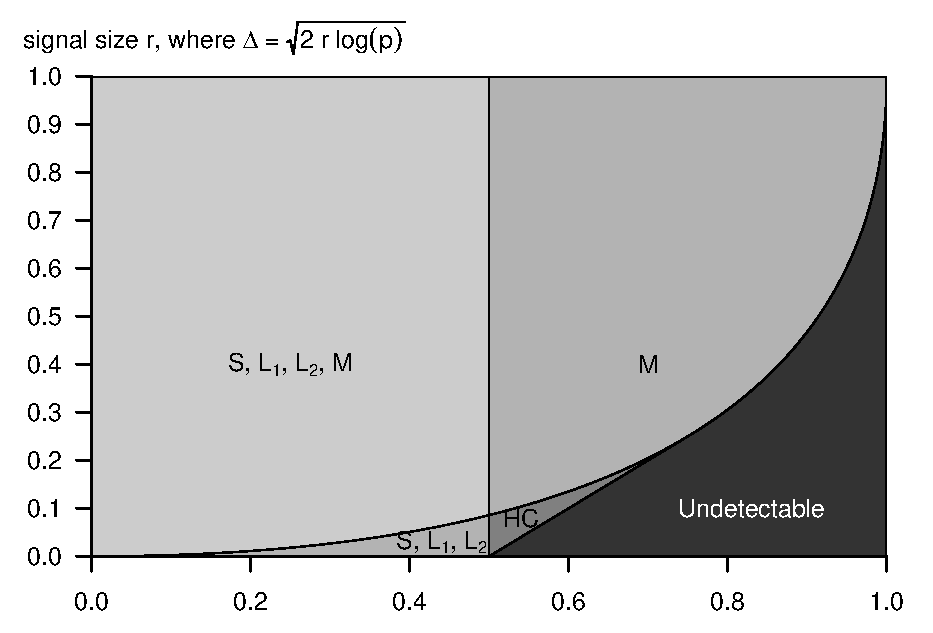
\includegraphics[width=0.7\textwidth]{figures/phase_diagram_signal_detection.eps}
      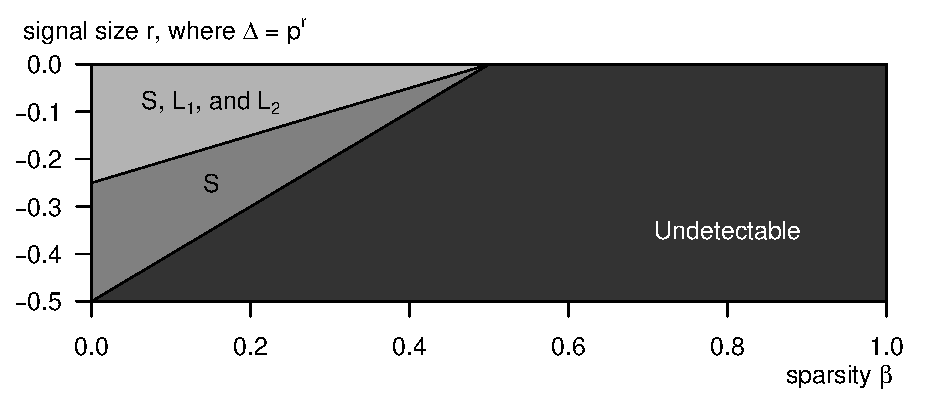
\includegraphics[width=0.7\textwidth]{figures/phase_diagram_signal_detection_vanishing_signals.eps}
      \caption{The phase diagrams of the sparse signal detection problem. 
      Signal size and sparsity are parametrized by $r$ and $\beta$, respectively.
      % Signal sparsity $|S|$ is parametrized by $\beta$. 
      % Signal sizes $\Delta$, parametrized by $r$, increases with dimension $p$ inside the upper panel, and decreases with $p$ inside the power panel.
      The diagrams illustrate the regions where the signal detection problem can be solved asymptotically by some of the commonly used statistics: the maximum ($M$), the sum-of-squares ($L_2$), the sum-of-absolute values ($L_1$), and the sum ($S$).
      In each region of the diagram, the annotated statistics can make the detection risk \eqref{eq:risk-detection} vanish, as dimension $p$ diverges. Conversely, the risks has liminf at least one.
      The detection problem is unsolvable for very sparse and weak signals in the undetectable regions.
      Notice that the $L_1$ and $L_2$ statistics are in fact sub-optimal for all sparsity levels.
      On the other hand, the max-statistic remains powerful for sparse signals ($\beta>1/2$), and is fully efficient when the problem is very sparse ($\beta\ge3/4$).
      The \ac{HC} statistic can detect signals in all configurations in the detectable regions.
      See text and Theorem \ref{thm:detection-optimality}.}
      \label{fig:phase-diagram-signal-detection}
\end{figure}


To the best of our knowledge, performance of simple statistics such as $L_1$, $L_2$ norms, and $S$ in this weak signal setting have not been reported in the literature perhaps due to a perceived lack of novelty.
Our first Theorem investigates the performance of these routine statistics for detecting sparse signals in high-dimensions, and summarizes the known results.

\begin{theorem} \label{thm:detection-optimality}
Consider the signal detection problem in the triangular array of Gaussian error models \eqref{eq:model-additive-Chapter3} where the sparsity is parametrized as in \eqref{eq:signal-sparsity-additive}.
\begin{itemize}
    \item For signals whose sizes are parametrized as in \eqref{eq:signal-size-additive}, the detection problem can be asymptotically solved in the sense of \eqref{eq:support-recovery-success} with $L_2$, $L_1$, or $S$ statistic when $\beta\le 1/2$; on the other hand, these statistics are asymptotically powerless in the sense of \eqref{eq:support-recovery-failure} when $\beta>1/2$.
    \item For small and dense signals whose signal sizes are parametrized as in \eqref{eq:signal-size-small}, the detection problem can be asymptotically solved in the sense of \eqref{eq:support-recovery-success} with $L_2$ or $L_1$ statistic when $\underline{r}>\beta/2-{1}/{4}$; on the other hand, these statistics are asymptotically powerless in the sense of \eqref{eq:support-recovery-failure} when $\overline{r}<\beta/2-{1}/{4}$.
    Further, tests based on the $S$ statistic can succeed asymptotically in the sense of \eqref{eq:support-recovery-success} when $\underline{r}>\beta-1/2$, hence attaining the boundary of detectability in \eqref{eq:detection-boundary-small-signals}.
\end{itemize}
\end{theorem}

Theorem \ref{thm:detection-optimality} is proved in Section \ref{sec:proofs} below.
We visualize the results in Theorem in Figure \ref{fig:phase-diagram-signal-detection}.
It is worth noting that the $\beta$-$r$ parameter regions where $L_1$ and $L_2$ statistics are asymptotically powerful coincide, and these statistics are theoretically suboptimal for both sparse regimes ($\beta>1/2$) and relatively dense regimes ($\beta\le 1/2$).

Ideas have been proposed to combine statistics that are powerful for different alternatives to create adaptive tests that maintain high power for at all sparsity levels.
Such adaptive tests can be constructed, for example, by leveraging the asymptotic independence of the sum- and supremum-type statistics \citep{hsing1995note}. 
Recently, \citet{xu2016adaptive} showed that for dependent observations under mixing and moment conditions, the sum-of-power-type statistics
\begin{equation}
    \widetilde{L}_q(x) = \sum_{i=1}^p x^q(i)
\end{equation} 
with distinct positive integer powers (i.e., $q=1,2,\ldots$) are asymptotically jointly independent, and proposed an adaptive test that monitors the minimium p-value of tests constructed with $\tilde{L}_q$'s.
This idea is further developed in \cite{wu2019adaptive} for generalized linear models and in \cite{he2018asymptotically} with U-statistics.

Optimality properties of such adaptive tests and the optimal choice of the $q$-combinations, however, remain open problems.
\cite{xu2016adaptive} suggested combine $q=1, 2, 3, \ldots, 6$, and  $q=\infty$, based empirical evidence from numerical experiments. 
Theorem \ref{thm:detection-optimality} here implies that, at least for detecting one-sided alternatives, the $\widetilde{L}_2$ statistic (i.e., $L_2$ norm) and the $L_1$ norm are asymptotically dominated by the $\widetilde{L}_1$ statistic (or equivalently, the sum $S$). Therefore it is sufficient to include only the latter in the construction of the adaptive test. 









%\newpage
\section{Sparse signal support recovery problems}
\label{sec:additive-error-model-boundaries}




Turning to support recovery problems in the Gaussian error model \eqref{eq:model-additive-Chapter3}, in the rest of this chapter
we will analyze the asymptotic performance limits in terms of the risk metrics for exact, exact-approximate, approximate-exact support recovery problems (i.e., \eqref{eq:risk-exact}, \eqref{eq:risk-exact-approx}, and \eqref{eq:risk-approx-exact}, respectively), as well as the probability of support recovery
\eqref{eq:risk-prob}.  We will also review the recent result for exact support recovery risk \eqref{eq:risk-approximate} by \cite{arias2017distribution}, to 
reveal a rather complete landscape of support recovery problems in high-dimensional Gaussian error models.


\begin{figure}
  \begin{center}
    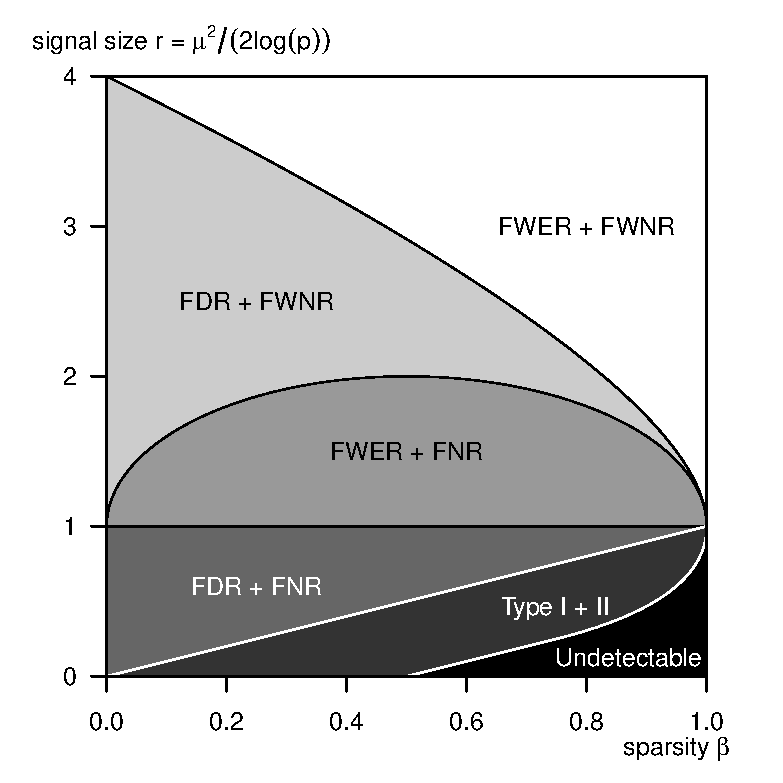
\includegraphics[width=0.7\textwidth]{./figures/theoretical_boundaries/phase_diagram_Gaussian_ALL_boundaries.eps}
  \end{center}
   \caption{The phase diagram of support recovery problems for the high-dimensional model \eqref{eq:model-additive-Chapter3}, illustrating the boundaries of the exact support recovery (FWER + FWNR; top curve; Theorem \ref{thm:Gaussian-error-exact-boundary}), the approximate-exact support recovery (FDR + FWNR; second curve from top; Theorem \ref{thm:Gaussian-error-approx-exact-boundary}), the exact-approximate support recovery (FWER + FNR; horizontal line $r=1$; Theorem \ref{thm:Gaussian-error-exact-approx-boundary}), and the approximate support recovery problems (FDR + FNR; tilted line $r=\beta$; Theorem \ref{thm:Gaussian-error-approx-boundary}). The signal detection problem (Type I + Type II errors of the global test; lower curve) was studied in Donoho and Jin (2004). In each region of the diagram and above, the annotated statistical risk can be made to vanish, as dimension $p$ diverges. Conversely, the risks has liminf at least one.}
   \label{fig:phase-Gaussian-errors}
\end{figure}

In the rest of this chapter, we restrict our attention to the class of thresholding procedures. Specifically, the lower bounds that we develop in 
Theorems \ref{thm:Gaussian-error-exact-boundary} through \ref{thm:Gaussian-error-approx-exact-boundary} below are only meant to apply to thresholding
 procedures.  Although it is intuitively appealing to consider only data-thresholding procedures in multiple testing problems, such procedures are not always optimal in more general settings. 
% Recently, \cite{arias2019detection} showed that thresholding procedures are in fact sub-optimal in the additive models \eqref{eq:model-additive} when errors have heavy (regularly-varying) tails. 
% Gao and Stoev [14] characterized the conditions under which thresholding procedures are optimal in the exact support recovery problem. 
% The optimality of data-thresholding procedures in terms of other statistical risks is an open problem that invites a dedicated investigation in a future study.
The optimality of thresholding procedures and the consequences of this restriction will be treated in Chapter \ref{chap:optimality}.


Figure \ref{fig:phase-Gaussian-errors} illustrates the rich landscape of phase transitions in support recovery for the various choices
of statistical risk for the family of thresholding estimators, established in the following sections.
We end this brief overview with a technical notion needed in order to state our main results.
We define a rate at which the nominal levels of FWER or FDR go to zero.
\begin{definition} \label{def:slowly-vanishing}
We say the nominal level of errors $\alpha = \alpha_p$ vanishes slowly, if
\begin{equation} \label{eq:slowly-vanishing-error}
    \alpha\to 0,\quad \text{and} \quad \alpha p^\delta\to\infty \text{  for any } \delta>0.
\end{equation}
\end{definition}
As an example, the sequence of nominal levels $\alpha_p = 1/\log{(p)}$ is slowly vanishing, while the sequence $\alpha_p = 1/\sqrt{p}$ is not.





\section{The exact support recovery problem}
\label{subsec:exact-support-recovery-Gaussian}

Our study of the exact support recovery risk \eqref{eq:risk-exact} begins with a brief review of existing results for the Hamming loss \eqref{eq:Hamming-loss}.
Indeed, as discussions in Section \ref{sec:asymptotics} suggest, the latter can be informative of the exact support recovery problems for models with independent components.

Inspired by the phase transition results for the signal detection problem, \cite{ji2012ups}, \citet{genovese2012comparison}, and \cite{jin2014optimality} derived interesting sharp results on support recovery problems in linear models under the Hamming loss $H(\widehat S, S)$.
Specifically, these papers establish minimax-type phase transition results in their respective settings. 
Under the sparsity parametrization in \eqref{eq:signal-sparsity-additive} and assuming equal signal sizes of ${(2r\log{p})^{1/2}}$, Hamming losses were shown to diverge to $+\infty$ when $r$ falls below the threshold
\begin{equation} \label{eq:strong-classification-boundary-Gaussian}
    f_{\mathrm{E}}(\beta) = (1 + (1 - \beta)^{1/2})^2,
\end{equation}
for any method of support estimation.
Conversely, under orthogonal, or near-orthogonal random designs, if $r>f_{\mathrm{E}}(\beta)$, they showed that the methods they proposed achieve vanishing Hamming loss.

Very recently, \citet{butucea2018variable}\; studied both asymptotics and non-asymptotics of support recovery problems in the additive noise model \eqref{eq:model-additive-Chapter3} under the assumption of equal signal sizes, using the Hamming loss.
Again, the analysis of asymptotic optimality focused on a newly proposed procedure which is very specific to the Gaussian model.
It is not at all clear if the optimality properties are a consequence of its mysterious construction.

We now show that commonly used and computationally efficient procedures can also be asymptotically optimal in the exact support recovery problem.

\begin{theorem} \label{thm:Gaussian-error-exact-boundary}
Consider the high-dimensional additive error model \eqref{eq:model-additive-Chapter3} under independent standard Gaussian errors, with signal sparsity and size as described in \eqref{eq:signal-sparsity-additive} and \eqref{eq:signal-size-additive}.
The function \eqref{eq:strong-classification-boundary-Gaussian} characterizes the phase transition of the exact support recovery problem.
Namely, the following two results hold.\\

{\rm (i)} If $\underline{r} > f_{\mathrm{E}}(\beta)$, then Bonferroni's, Sid\'ak's, Holm's, and Hochberg's procedures with slowly vanishing  nominal FWER levels 
(as defined in Definition \ref{def:slowly-vanishing}) all achieve asymptotically exact support recovery in the sense of \eqref{eq:support-recovery-success}. \\

{\rm (ii)} Conversely, if $\overline{r} < f_{\mathrm{E}}(\beta)$, then for any thresholding procedure $\widehat{S}_p$, we have $\P[\widehat{S}_p=S_p]\to0$.
Therefore, in view of Lemma \ref{lemma:risk-exact-recovery-probability}, exact support recovery asymptotically fails for all thresholding procedures in the sense of \eqref{eq:support-recovery-failure}.
\end{theorem}

We illustrate this result with a $\beta$-$r$ phase diagram in Figure \ref{fig:phase-Gaussian-errors}.  Theorem \ref{thm:Gaussian-error-exact-boundary} is in 
fact a special case of the more general Theorem \ref{thm:sufficient}, below, which covers dependent as well as Gaussain and non-Gaussian errors.  We will study the {\em exact support recovery} problem in greater detail and generality in Chapter \ref{chap:exact-support-recovery}. 


\section{The approximate support recovery problem}
\label{subsec:approx-support-recovery-Gaussian}

\cite{arias2017distribution} studied the performance of the Benjamini-Hochberg procedure \citep{benjamini1995controlling} and a stripped-down version of the Cand\'es-Barber procedure \citep{barber2015controlling} in approximate support recovery problems when the components of the noise term $\epsilon$ in \eqref{eq:model-additive-Chapter3} have independent and symmetric distributions.
A phase transition phenomenon for the approximate support recovery risk \eqref{eq:risk-approximate} was established in the Gaussian additive error model, where the two aforementioned methods are both shown to be asymptotically optimal.

The analysis therein, however, assumed equal signal sizes for the alternatives.
We generalize the main results of \citet{arias2017distribution} to allow for unequal signal sizes. 
The key to establishing this generalization is a monotonicity property of the \ac{BH} procedure, presented in the following 
Section \ref{sec:BH-monotonicity}. Namely, the power of the \ac{BH} procedure in terms of FNR monotonically increases for stochastically 
larger alternatives. This fact will be formalized in Lemma \ref{lemma:monotonicity-BH-procedure}, and may be of independent interest.


\begin{theorem} \label{thm:Gaussian-error-approx-boundary}
In the context of Theorem \ref{thm:Gaussian-error-exact-boundary}, the function 
\begin{equation} \label{eq:approx-boundary-Gaussian}
    f_{\mathrm{A}}(\beta) = \beta
\end{equation}
characterizes the phase transition of approximate support recovery problem.  Specifically the following two results hold.\\

{\rm (i)} If $\underline{r} > f_{\mathrm{a}}(\beta)$, then the Benjamini-Hochberg procedure (defined in Section \ref{sec:statistical-procedures}) with slowly 
vanishing nominal FDR levels (as defined in Definition \ref{def:slowly-vanishing}) achieves asymptotically approximate support recovery in the sense of \eqref{eq:support-recovery-success}.\\ 

{\rm (ii)}
Conversely, if $\overline{r} < f_{\mathrm{a}}(\beta)$, then approximate support recovery asymptotically fails in the sense of \eqref{eq:support-recovery-failure} for all thresholding procedures.
\end{theorem}


\begin{proof}[Necessary condition in Theorem \ref{thm:Gaussian-error-approx-boundary}]
We first show part {\rm (ii)}.  That is, when $\overline{r} < \beta$, no thresholding procedure is able to achieve approximate support recovery.
The arguments are similar to that in Theorem 1 of \cite{arias2017distribution}, although we allow for unequal signal sizes. 

Denote the distributions of $\mathrm{N}(0,1)$, $\mathrm{N}(\underline{\Delta}, 1)$, and $\mathrm{N}((\overline{\Delta}, 1)$ as $F_0$, $F_{\underline{a}}$, and $F_{\overline{a}}$ respectively.

% We first show the necessary condition, i.e., when $\overline{r}<\beta$, approximate support recovery cannot be achieved with any thresholding procedure.
% In particular, we show that the liminf of the sum of FDP and NDP is at least 1.

Recall that thresholding procedures are of the form
$$
\widehat{S}_p = \left\{i\,|\,x(i) > t_p(x)\right\}.
$$
Denote $\widehat{S} := \left\{i\,|\,x(i) > t_p(x)\right\}$, and $\widehat{S}(u) := \left\{i\,|\,x(i) > u\right\}$.
For any threshold $u\ge t_p$ we must have $\widehat{S}(u)\subseteq\widehat{S}$, and hence
\begin{equation} \label{eq:approx-boundary-proof-FDP-Gaussian}
    \text{FDP} := \frac{|\widehat{S}\setminus{S}|}{|\widehat{S}|} \ge \frac{|\widehat{S}\setminus{S}|}{|\widehat{S}\cup{S}|} = \frac{|\widehat{S}\setminus{S}|}{|\widehat{S}\setminus{S}| + |S|} \ge
    \frac{|\widehat{S}(u)\setminus{S}|}{|\widehat{S}(u)\setminus{S}| + |S|}.
\end{equation}
On the other hand, for any threshold $u\le t_p$ we must have $\widehat{S}(u)\supseteq\widehat{S}$, and hence
\begin{equation} \label{eq:approx-boundary-proof-NDP-Gaussian}
    \text{NDP} := \frac{|{S}\setminus\widehat{S}|}{|{S}|} \ge 
    \frac{|{S}\setminus\widehat{S}(u)|}{|{S}|}.
\end{equation}
Since either $u\ge t_p$ or  $u\le t_p$ must take place, putting \eqref{eq:approx-boundary-proof-FDP-Gaussian} and \eqref{eq:approx-boundary-proof-NDP-Gaussian} together, we have
\begin{equation} \label{eq:approx-boundary-proof-converse-1-Gaussian}
    \text{FDP} + \text{NDP} 
    \ge \frac{|\widehat{S}(u)\setminus{S}|}{|\widehat{S}(u)\setminus{S}|+|{S}|} \wedge \frac{|{S}\setminus\widehat{S}(u)|}{|{S}|},
\end{equation}
for any $u$.
Therefore it suffices to show that for a suitable choice of $u$, the RHS of \eqref{eq:approx-boundary-proof-converse-1-Gaussian} converges to 1 in probability; the desired conclusion on FDR and FNR follows by the dominated convergence theorem.

Let $t^* = \sqrt{2q\log{p}}$ for some fixed $q$, we obtain an estimate of the tail probability by Mill's ratio \eqref{eq:Mills-ratio}, 
\begin{equation}
    \overline{F_0}(t^*) 
    \sim \frac{1}{t^*}\phi(t^*)
    = \frac{1}{2\sqrt{\pi q\log{p}}} p^{-q}, \label{eq:approx-boundary-proof-null-tail-prob-Gaussian}
\end{equation}
where $a_p\sim b_p$ is taken to mean $a_p/b_p\to 1$.
Observe that $|\widehat{S}(t^*)\setminus{S}|$ has distribution $\text{Binom}(p-s, \overline{F_0}(t^*))$ where $s=|S|$, denote $X = X_p := {|\widehat{S}(t^*)\setminus{S}|}/{|S|}$, and we have 
$$
\mu := \E\left[X\right] = \frac{(p-s)\overline{F_0}(t^*)}{s},
\quad \text{and} \quad
\var\left(X\right) = \frac{(p-s)\overline{F_0}(t^*){F_0}(t^*)}{s^2} \le \mu/s.
$$
Therefore for any $M>0$, we have, by Chebyshev's inequality,
\begin{equation}
    \P\left[X < M\right] 
    \le \P\left[\left|X-\mu\right| > \mu - M\right]
    \le \frac{\mu/s}{(\mu-M)^2}
    = \frac{1/(\mu s)}{(1-M/\mu)^2}. \label{eq:approx-boundary-proof-converse-2-Gaussian}
\end{equation}
Now, from the expression of $\overline{F_0}(t^*)$ in \eqref{eq:approx-boundary-proof-null-tail-prob-Gaussian}, we obtain
$$
\mu = (p^\beta - 1)\overline{F_0}(t^*) \sim \frac{1}{2\sqrt{\pi q\log{p}}} p^{\beta-q}.
$$
Since $\overline{r}<\beta$, we can pick $q$ such that $\overline{r}<q<\beta$. 
In turn, we have $\mu \to\infty$, as $p\to\infty$.
Therefore the last expression in \eqref{eq:approx-boundary-proof-converse-2-Gaussian} converges to 0, and we conclude that $X\to\infty$ in probability, and hence
\begin{equation} \label{eq:approx-boundary-proof-converse-3-Gaussian}
\frac{|\widehat{S}(t^*)\setminus{S}|}{|\widehat{S}(t^*)\setminus{S}|+|{S}|} 
= \frac{X}{X+1} \to 1 \quad \text{in probability}.
\end{equation}

On the other hand, we show that with the same choice of $u = t^*$, we have,
\begin{equation} \label{eq:approx-boundary-proof-converse-4-Gaussian}
    \frac{|{S}\setminus\widehat{S}(t^*)|}{|{S}|}\to 1 \quad \text{in probability}.
\end{equation}
By the stochastic monotonicity of Gaussian location family \eqref{eq:stochastic-monotonicity-Gaussian}, we have the following lower bound for the probability of missed detection for each signal $\mu(i)$, $i\in S$, 
\begin{equation} \label{eq:approx-boundary-proof-converse-5-Gaussian}
    \P[\mathrm{N}(\mu(i), 1) \le t^*] \ge F_{\overline{a}}(t^*).
\end{equation}
Since $|{S}\setminus\widehat{S}(t^*)|$ can be written as the sum of $s$ independent Bernoulli random variables,
\begin{equation*}
    |{S}\setminus\widehat{S}(t^*)| = \sum_{i\in S} \mathbbm{1}_{(-\infty, t^*]}(x(i)),
\end{equation*}
using with \eqref{eq:approx-boundary-proof-converse-5-Gaussian}, we conclude that $|{S}\setminus\widehat{S}(t^*)| \stackrel{\mathrm{d}}{\ge} \text{Binom}(s, {F_{\overline{a}}}(t^*))$.
Finally, we know that ${F_{\overline{a}}}(t^*)$ converges to 1 by our choice of diverging $t^*$, and the necessary condition is shown.
\end{proof}


\begin{proof}[Sufficient condition in Theorem \ref{thm:Gaussian-error-approx-boundary}]
We now turn to the sufficient condition, i.e., part {\rm (i)}. That is, when $\underline{r} > \beta$, the Benjamini-Hochberg procedure with 
slowly vanishing FDR levels achieves asymptotic approximate support recovery.

The FDR vanishes by our choice of $\alpha$ and the FDR-controlling property of the BH procedure \citep{benjamini1995controlling}.
It only remains to show that FNR also vanishes.

To do so we compare the FNR under the alternative specified in Theorem \ref{thm:Gaussian-error-approx-boundary} to one with all of the signal sizes equal to $\underline{\Delta}$.
By Lemma \ref{lemma:monotonicity-BH-procedure}, it suffices to show that the FNR under the BH procedure in this setting vanishes.
Let $x(i)$ be vectors of independent observations with $p-s$ nulls having standard Gaussian distributions, and $s$ signals having $\mathrm{N}(\underline{\Delta}, 1)$ distributions.

Denote the null and the alternative distributions as $F_0$ and $F_{a}$ respectively.
Let $\widehat{G}$ denote the empirical survival function as in \eqref{eq:empirical-tail-distribution}.
Define the empirical survival functions for the null part and signal part
\begin{equation} \label{eq:empirical-survival-null-signal-Gaussian}
    \widehat{W}_\text{null}(t) = \frac{1}{p-s}\sum_{i\not\in S}\mathbbm{1}\{x(i) \ge t\},
    \quad
    \widehat{W}_\text{signal}(t) = \frac{1}{s}\sum_{i\in S}\mathbbm{1}\{x(i) \ge t\},
\end{equation}
where $s=|S|$, so that
$$
\widehat{G}(t) = \frac{p-s}{p}\widehat{W}_\text{null}(t) + \frac{s}{p}\widehat{W}_\text{signal}(t).
$$

We need the following result to describe the deviations of the empirical distributions.
\begin{lemma}[Theorem 1 of \citet{eicker1979asymptotic}] \label{lemma:empirical-process}
Let $Z_1,\ldots,Z_k$ be iid with continuous survival function $Q$.
Let $\widehat{Q}_k$ denote their empirical survival function and define 
$\xi_k = \sqrt{2\log{\log{(k)}}/k}$ for $k \ge 3$. 
Then
$$
\frac{1}{\xi_k}\sup_z\frac{|\widehat{Q}_k(z) - Q(z)|}{\sqrt{Q(z)(1 - Q(z))}} \to 1,
$$
in probability as $k \to \infty$.
In particular,
$$
\widehat{Q}_k(z) = Q(z) + O_\P\left(\xi_k\sqrt{Q(z)(1 - Q(z))}\right),
$$
uniformly in z.
\end{lemma}

Apply Lemma \ref{lemma:empirical-process} to the two summands in $\widehat{G}$, we obtain
$\widehat{G}(t) = G(t) + \widehat{R}(t)$,
where 
\begin{equation} \label{eq:empirical-process-mean-Gaussian}
    G(t) = \frac{p-s}{p}\overline{F_0}(t) + \frac{s}{p}\overline{F_a}(t),
\end{equation}
and 
\begin{equation} \label{eq:empirical-process-residual-Gaussian}
    \widehat{R}(t) = O_\P\left(\xi_p\sqrt{\overline{F_0}(t)F_0(t)} + \frac{s}{p}\xi_s\sqrt{\overline{F_a}(t)F_a(t)}\right),
\end{equation}
uniformly in $t$.

Recall (see proof of Lemma \ref{lemma:monotonicity-BH-procedure}) that the BH procedure is the thresholding procedure with threshold set at 
\begin{equation} \label{eq:approx-boundary-proof-tau-Gaussian}
    \tau = \inf\{t\,|\,\overline{F_0}(t)\le\alpha\widehat{G}(t)\}. 
    %= \min\{t\,|\,\overline{F_0}(t)=\alpha\widehat{G}(t)\}.
\end{equation}
The NDP may also be re-written as 
$$
\text{NDP} = \frac{|{S}\setminus\widehat{S}|}{|{S}|} = \frac{1}{s}\sum_{i\in S}\mathbbm{1}\{x(i) < \tau\} = 1 - \widehat{W}_\text{signal}(\tau),
$$
so that it suffices to show that 
\begin{equation} \label{eq:approx-boundary-proof-sufficient-1-Gaussian}
    \widehat{W}_\text{signal}(\tau)\to 1
\end{equation} in probability.
Applying Lemma \ref{lemma:empirical-process} to $\widehat{W}_\text{signal}$, we know that 
$$
\widehat{W}_\text{signal}(\tau) = \overline{F_a}(\tau) + O_\P\left(\xi_s\sqrt{\overline{F_a}(\tau)F_a(\tau)}\right) = \overline{F_a}(\tau) + o_\P(1).
$$
So it suffices to show that $F_a(\tau)\to 0$ in probability.
Now let $t^* = \sqrt{2q\log(p)}$ for some $q$ such that $\beta<q<\underline{r}$.
We have 
\begin{equation} \label{eq:approx-boundary-proof-sufficient-2-Gaussian}
    F_a(t^*) 
    = \Phi(t^* - \underline{\Delta}) 
    = \Phi(\sqrt{2(q - \underline{r})\log{p}}) \to 0. 
\end{equation}
Hence in order to show \eqref{eq:approx-boundary-proof-sufficient-1-Gaussian}, it suffices to show 
\begin{equation} \label{eq:approx-boundary-proof-sufficient-3-Gaussian}
    \P\left[\tau \le t^*\right] \to 1.
\end{equation}
By \eqref{eq:empirical-process-mean-Gaussian}, the mean of the empirical process $\widehat{G}$ evaluated at $t^*$ is
\begin{equation} \label{eq:approx-boundary-proof-sufficient-4-Gaussian}
    G(t^*) = \frac{p-s}{p}\overline{F_0}(t^*) + \frac{s}{p}\overline{F_a}(t^*).
\end{equation}
The first term, using Relation \eqref{eq:approx-boundary-proof-null-tail-prob-Gaussian}, is asymptotic to $p^{-q}L(p)$, where $L(p)$ is the logarithmic term in $p$.
The second term, since $\overline{F_a}(t^*)\to 1$ by Relation \eqref{eq:approx-boundary-proof-sufficient-2-Gaussian}, is asymptotic to $p^{-\beta}$.
Therefore, $G(t^*) \sim p^{-q}L(p) + p^{-\beta} \sim p^{-\beta}$, since 
$p^{\beta-q}L(p)\to0$ where $q>\beta$.

The fluctuation of the empirical process at $t^*$, by Relation \eqref{eq:empirical-process-residual-Gaussian}, is 
\begin{align*}
    \widehat{R}(t^*) 
    &= O_\P\left(\xi_p\sqrt{\overline{F_0}(t^*)F_0(t^*)} + \frac{s}{p}\xi_s\sqrt{\overline{F_a}(t^*)F_a(t^*)}\right)\\
    &= O_\P\left(\xi_p\sqrt{\overline{F_0}(t^*)}\right) + o_\P\left(p^{-\beta}\right).
\end{align*}
By \eqref{eq:approx-boundary-proof-null-tail-prob-Gaussian} and the expression for $\xi_p$, the first term is $O_\P\left(p^{-(q+1)/2}L(p)\right)$ where $L(p)$ is a poly-logarithmic term in $p$.
Since $\beta<\min\{q,1\}$, we have $\beta<(q+1)/2$, and hence $\widehat{R}(t^*) = o_\P(p^{-\beta})$.

Putting the mean and the fluctuation of $\widehat{G}(t^*)$ together, we obtain
$$
\widehat{G}(t^*) = G(t^*) + \widehat{R}(t^*) \sim_\P G(t^*) \sim p^{-\beta},
$$
and therefore, together with \eqref{eq:approx-boundary-proof-null-tail-prob-Gaussian}, we have
$$
\overline{F_0}(t^*)/\widehat{G}(t^*) = p^{\beta-q}L(p)(1+o_{\P}(1)),
$$
which is eventually smaller than the FDR level $\alpha$ by the assumption \eqref{eq:slowly-vanishing-error} and the fact that $\beta<q$.
That is, 
$$
\P\left[\overline{F}_0(t^*) / \widehat{G}(t^*) < \alpha\right] \to 1.
$$
By definition of $\tau$ (recall \eqref{eq:approx-boundary-proof-tau-Gaussian}), this implies that $\tau \le t^*$ with probability tending to 1, and \eqref{eq:approx-boundary-proof-sufficient-3-Gaussian} is shown.
The proof for the sufficient condition is complete.
\end{proof}


\section{Monotonicity of the Benjamini-Hochberg procedure}
\label{sec:BH-monotonicity}

As promised in the previous section, we make a connection between power of the \ac{BH} procedure and the stochastic ordering of distributions under the alternative.
This natural result seems new. 

\begin{lemma}[Monotonicity of the BH procedure] \label{lemma:monotonicity-BH-procedure}
Consider $p$ independent observations $x(i)$, $i\in\{1,\ldots,p\}$, where the $(p-s)$ coordinates in the null part have common distribution $F_0$, and the remaining $s$ signals have alternative distributions $F^{i}_j$, $i\in S$, respectively.
Compare the two alternatives $j\in\{1,2\}$, where the distributions in Alternative 2 are stochastically larger than those in Alternative 1, i.e.,
\begin{equation*}
    F^{i}_2(t) \le F^{i}_1(t), \quad \text{for all} \;\; t\in\R, \; \text{and for all} \;\; i\in S.
\end{equation*}
If the BH procedure is applied at the same nominal level of FDR, then the FNR of the \ac{BH} procedure under Alternative 2 is bounded above by the FNR under Alternative 1.
Further, the threshold of the \ac{BH} procedure under Alternative 2 is stochastically smaller than that under Alternative 1.
\end{lemma}

Loosely put, the power of the BH procedure is monotone increasing with respect to the stochastic ordering of the alternatives, yet (the distribution of) the \ac{BH} threshold is monotone decreasing in the distributions of the alternatives.

\begin{proof}[Lemma \ref{lemma:monotonicity-BH-procedure}]
We first re-express the BH procedure in a different form.
Recall that on observing $x(i)$, $i\in\{1,\ldots,p\}$, the BH procedure is the thresholding procedure with threshold set at $x_{[i^*]}$, where $i^* := \max\{i\,|\,\overline{F_0}(x_{[i]})\le \alpha i/p\}$, and $x_{[1]}\ge\ldots\ge x_{[p]}$ are the order statistics.

Let $\widehat{G}$ denote the left-continuous empirical survival function
\begin{equation} \label{eq:empirical-tail-distribution}
    \widehat{G}(t) = \frac{1}{p}\sum_{i=1}^p\mathbbm{1}\{x(i) \ge t\}.
\end{equation}
By the definition, we know that $\widehat{G}(x_{[i]}) = i/p$.
Therefore, by the definition of $i^*$, we have
\begin{equation*} 
    \overline{F_0}(x_{[i]}) > \alpha\widehat{G}(x_{[i]}) = \alpha i/p \quad \text{for all }i>i^*.
\end{equation*}
Since $\widehat{G}$ is constant on $(x_{[i^*+1]}, x_{[i^*]}]$, the fact that 
$\overline{F_0}(x_{[i^*]}) \le \alpha\widehat{G}(x_{[i^*]})$ and $\overline{F_0}(x_{[i^*+1]}) > \alpha\widehat{G}(x_{[i^*+1]})$ implies that $\alpha\widehat{G}$ and $\overline{F_0}$ must ``intersect'' on the interval by continuity of $F_0$.
We denote this ``intersection'' as
\begin{equation} \label{eq:approx-boundary-proof-tau}
    \tau = \inf\{t\,|\,\overline{F_0}(t)\le\alpha\widehat{G}(t)\}. 
    %= \min\{t\,|\,\overline{F_0}(t)=\alpha\widehat{G}(t)\}.
\end{equation}
Note that $\tau$ cannot be equal to $x_{[i^*+1]}$ since $\overline{F}_0$ is c\`adl\`ag.
Since there is no observation in $[\tau, x_{[i^*]})$, we can write the BH procedure as the thresholding procedure with threshold set at $\tau$.

Now, denote the observations under Alternatives 1 and 2 as $x_1(i)$ and $x_2(i)$.
Since $x_2(i)$ stochastically dominates $x_1(i)$ for all $i\in\{1,\ldots,p\}$, there exists a coupling $(\widetilde{x}_1, \widetilde{x}_2)$ of $x_1$ and $x_2$ such that 
% $\widetilde{x}_1(i) = \widetilde{x}_2(i)$ for $i\in S^c$, and 
$\widetilde{x}_1(i) \le \widetilde{x}_2(i)$ almost surely for all $i$.
We will replace $\widetilde{x}_1$ and $\widetilde{x}_2$ with $x_1$ and $x_2$ in what follows.
Since we will compare the FNR's, i.e., expectations with respect to the marginals of ${x}$'s in the last step, this replacement does not affect the conclusions.
To simplify notation, we still write $x_1$ and $x_2$ in place of $\widetilde{x}_1$ and $\widetilde{x}_2$.

Let $\widehat{G}_k$ be the left-continuous empirical survival function under Alternative $k$, i.e.,
\begin{equation} \label{eq:empirical-survival}
    \widehat{G}_k(t) = \frac{1}{p}\sum_{i=1}^p\mathbbm{1}\{x_k(i) \ge t\}, \quad k\in\{1,2\}.
\end{equation}
We define the BH thresholds $\tau_1$ and $\tau_2$ by replacing $\widehat{G}$ in \eqref{eq:approx-boundary-proof-tau} with $\widehat{G}_1$ and $\widehat{G}_2$, respectively.
Denote the set estimates of signal support $\widehat{S}_k = \{i\,|\,x_k(i)\ge\tau_k\}$ by the BH procedure.
We claim that 
\begin{equation} \label{eq:monotonicity-BH-procedure-thresholds}
    \tau_2 \le \tau_1 \quad \text{with probability } 1.
\end{equation}

Indeed, by definition of the empirical survival function \eqref{eq:empirical-survival} and the fact that $x_1(i) \le x_2(i)$ almost surely for all $i$,  we have $\widehat{G}_1(t) \le \widehat{G}_2(t)$ for all $t$.
Hence, $\overline{F_0}(t)\le\alpha\widehat{G}_1(t)$ implies $\overline{F_0}(t)\le\alpha\widehat{G}_2(t)$, and Relation \eqref{eq:monotonicity-BH-procedure-thresholds} follows from the definition of $\tau$ in \eqref{eq:approx-boundary-proof-tau}.
The claim of stochastic ordering of the \ac{BH} thresholds in Lemma \ref{lemma:monotonicity-BH-procedure} follows from \eqref{eq:monotonicity-BH-procedure-thresholds}.

Finally, when $\tau_2 \le \tau_1$, we have $\tau_2 \le \tau_1 \le x_1(i) \le x_2(i)$ with probability 1 for all $i\in\widehat{S}_1$.
Therefore, it follows that $\widehat{S}_1 \subseteq \widehat{S}_2$ and hence $|S\setminus\widehat{S}_2| \le |S\setminus\widehat{S}_1|$ almost surely. 
The first conclusion in Lemma \ref{lemma:monotonicity-BH-procedure} follows from the last inequality.
\end{proof}




\section{The exact-approximate support recovery problem}
\label{subsec:exact-approx-support-recovery-Gaussian}

We now derive two new asymptotic phase transition results for the \emph{asymmetric} statistical risks, \eqref{eq:risk-exact-approx} and \eqref{eq:risk-approx-exact}, in the Gaussian error models.
As discussed in Section \ref{sec:risks}, the exact-approximate support recovery risk is the natural criteria when considering the marginal power of discovery while controlling for family-wise error rates in applications such as GWAS.

Although there have been discussions of weighted sums of type I and type II errors in the literature (see, e.g., Genovese and Wasserman \citep{genovese2002operating} Section 6, where the authors sought to minimize $\textrm{FDR} + \lambda\textrm{FNR}$), asymptotic limits were not discussed.
We point out that the asymptotic limits for the unequally-weighted risks are no different from the equally-weighted risk, so long as $\lambda$ is bounded away from zero and infinity.
This is because $\textrm{FDR} + \lambda\textrm{FNR}$ vanishes if and only if both FDR and FNR vanish; conversely, non-vanishing FDR and FNR is equivalent to non-vanishing weighted sums.
Therefore, a different phase transition would only arise if we weight the type I and type II errors by combining family-wise error metrics with marginal error rates.

The next theorem describes the phase transition in the exact-approximate support recovery problem.

\begin{theorem} \label{thm:Gaussian-error-exact-approx-boundary}
In the context of Theorem \ref{thm:Gaussian-error-exact-boundary}, the function 
\begin{equation} \label{eq:exact-approx-boundary-Gaussian}
    f_{\mathrm{EA}}(\beta) = 1
\end{equation}
characterizes the phase transition of exact-approximate support recovery problem.  Namely, the following two results hold.\\

{\rm (i)} If $\underline{r} > f_{\mathrm{EA}}(\beta)$, then the procedures listed in Theorem \ref{thm:Gaussian-error-exact-boundary} with slowly vanishing nominal FWER levels (as defined in Definition \ref{def:slowly-vanishing}) achieve asymptotically exact-approximate support recovery in the sense of \eqref{eq:support-recovery-success}. \\

{\rm (ii)} Conversely, if $\overline{r} < f_{\mathrm{EA}}(\beta)$, then for any thresholding procedure $\widehat{S}$, the exact-approximate support recovery fails in the sense of \eqref{eq:support-recovery-failure}.
\end{theorem}

The phase transition boundary \eqref{eq:exact-approx-boundary-Gaussian} is visualized in Figure \ref{fig:phase-Gaussian-errors}. The proof of this result
uses ideas from the proof of Theorem \ref{thm:Gaussian-error-approx-boundary} and is substantially shorter.

\begin{proof}[Theorem \ref{thm:Gaussian-error-exact-approx-boundary}]
We first show the sufficient condition. 
Vanishing FWER is guaranteed by the properties of the procedures, and we only need to show that FNR also goes to zero. 
Similar to the proof of Theorem \ref{thm:Gaussian-error-approx-boundary}, it suffices to show that
\begin{equation} \label{eq:additive-error-exact-approx-boundary-proof-sufficient-1}
    \text{NDP} = 1 - \widehat{W}_\text{signal}(t_p) \to 0,
\end{equation}
where $t_p$ is the threshold of Bonferroni's procedure.

Since $\alpha$ vanishes slowly (see Definition \ref{eq:slowly-vanishing-error}), for any $\delta>0$, we have $p^{-\delta}=o(\alpha)$.
Therefore, we have $-\log\alpha\le\delta\log{p}$ for large $p$, and
\begin{equation*} 
    1 \le \limsup_{p\to\infty}\frac{2\log{p} - 2\log{\alpha}}{2\log{p}} \le 1+\delta,
\end{equation*}
for any $\delta>0$.
Therefore, by the expression for normal quantiles, we know that 
$$
t_p=F^\leftarrow(1-\alpha/p)\sim(2\log{p}-2\log{\alpha})^{1/2} \sim(2\log{p})^{1/2}.
$$

Since $\underline{r}>f_{\mathrm{EA}}(\beta)=1$, we can pick $q$ such that $1<q<\underline{r}$.
Let $t^* = \sqrt{2q\log{p}}$, we know that $t_p<t_p^*$ for large $p$.
Therefore for large $p$, we have
$$
\widehat{W}_\text{signal}(t_p) \ge \widehat{W}_\text{signal}(t^*) \ge \overline{F_a}(t^*) + o_\P(1),
$$
where $\overline{F_a}$ is the survival function of $\mathrm{N}(\sqrt{2\underline{r}\log{p}}, 1)$; the last inequality follows from the stochastic monotonicity of the Gaussian location family \eqref{eq:stochastic-monotonicity-Gaussian}, and Lemma \ref{lemma:empirical-process}.
Indeed, by our choice of $q<\underline{r}$, we obtain
$$
F_a(t^*) = \Phi\left(\sqrt{2(q-\underline{r})\log{p}}\right)\to0,
$$
and \eqref{eq:additive-error-exact-approx-boundary-proof-sufficient-1} is shown. 
This completes the proof of the sufficient condition.

The proof of the necessary condition follows similar structure as in the proof of Theorem \ref{thm:Gaussian-error-approx-boundary}, and uses the lower bound
\begin{equation} \label{eq:additive-error-exact-approx-boundary-proof-necessary-1}
    \mathrm{FWER}(\mathcal{R}) + \mathrm{FNR}(\mathcal{R}) \ge \P\left[\max_{i\in S^c}x(i)>u\right] \wedge \E\left[\frac{|S\setminus \widehat{S}(u)|}{|S|}\right],
\end{equation}
which holds for any arbitrary thresholding procedure $\mathcal{R}$ and arbitrary real $u\in\R$.

By the assumption that $\overline{r}<f_{\mathrm{EA}}(\beta)=1$, we can pick $q$ such that $\overline{r}<q<1$ and let $u = t^*=\sqrt{2q\log{p}}$ in \eqref{eq:additive-error-exact-approx-boundary-proof-necessary-1}.
By relative stability of iid Gaussian random variables \eqref{eq:relative-stability-Gaussian-maxima}, we have
\begin{equation} \label{eq:additive-error-exact-approx-boundary-proof-necessary-2}
    \P\left[\frac{\max_{i\in S^c} x(i)}{\sqrt{2\log{p}}} > \frac{t^*}{\sqrt{2\log{p}}}\right] \to 1.
\end{equation}
since the first fraction in \eqref{eq:additive-error-exact-approx-boundary-proof-necessary-2} converges to 1, while the second converges to $q<1$.
Therefore, the first term on the right-hand side of \eqref{eq:additive-error-exact-approx-boundary-proof-necessary-1} converges to 1.

On the other hand, by the stochastic monotonicity of Gaussian location family \eqref{eq:stochastic-monotonicity-Gaussian}, the probability of missed detection for each signal is lower bounded by $\P[Z+\mu(i) \le t^*] \ge F_{\overline{a}}(t^*)$, where $Z$ is a standard Gaussian r.v., and $F_{\overline{a}}$ is the cdf of $\mathrm{N}(\sqrt{2\overline{r}\log{p}}, 1)$.
Therefore, $|{S}\setminus\widehat{S}(t^*)| \stackrel{\mathrm{d}}{\ge} \text{Binom}(s, {F_{\overline{a}}}(t^*))$, and it suffices to show that ${F_{\overline{a}}}(t^*)$ converges to 1.
Indeed,
\begin{equation*}
    {F_{\overline{a}}}(t^*) = \Phi(\sqrt{2(q-\overline{r})\log{p}}) \to 1,
\end{equation*}
by our choice of $q>\overline{r}$.
Hence both quantities in the minimum on the right-hand side of \eqref{eq:additive-error-exact-approx-boundary-proof-necessary-1} converge to 1 in the limit, and the necessary condition is shown.
\end{proof}





\begin{remark}
The boundary \eqref{eq:exact-approx-boundary-Gaussian} was briefly suggested by \citet{arias2017distribution}.
Unfortunately, it was falsely claimed that the boundary characterized the phase transition of the \emph{exact} support recovery problem, and the alleged proof was left as an ``exercise to the reader''.
This exercise was completed in Chapter \ref{chap:exact-support-recovery}, where the correct boundary \eqref{eq:exact-boundary-chisquared} was identified. 

Theorem \ref{thm:Gaussian-error-exact-approx-boundary} here shows that the boundary \eqref{eq:exact-approx-boundary-Gaussian} \emph{does} exist, though for the slightly different \emph{exact-approximate} support recovery problem.
As we will see in Section \ref{sec:chisq-boundaries}, the boundary \eqref{eq:exact-approx-boundary-Gaussian} also applies to the exact-approximate support recovery problem in chi-square models \eqref{eq:model-chisq}.
\end{remark}

\section{The approximate-exact support recovery problem}
\label{subsec:aprox-exact-support-recovery-Gaussian}

The last phase transition is in terms of the approximate-exact support recovery risk
\eqref{eq:risk-approx-exact}.

\begin{theorem} \label{thm:Gaussian-error-approx-exact-boundary}
In the context of Theorem \ref{thm:Gaussian-error-exact-boundary}, the function 
\begin{equation} \label{eq:approx-exact-boundary-Gaussian}
    f_{\mathrm{AE}}(\beta) = \left(\sqrt{\beta} + \sqrt{1-\beta}\right)^2
\end{equation}
characterizes the phase transition of approximate-exact support recovery problem.  Namely, the following two results 
hold.\\

{\rm (i)} If $\underline{r} > f_{\mathrm{AE}}(\beta)$, then the Benjamini-Hochberg procedure with slowly vanishing nominal FDR levels (as defined in Definition \ref{def:slowly-vanishing}) achieves asymptotically approximate-exact support recovery in the sense of \eqref{eq:support-recovery-success}. \\

{\rm (ii)} Conversely, if $\overline{r} < f_{\mathrm{AE}}(\beta)$, then for any thresholding procedure $\widehat{S}$, the approximate-exact support recovery fails in the sense of \eqref{eq:support-recovery-failure}.
\end{theorem}

%Theorem \ref{thm:Gaussian-error-approx-exact-boundary} is proved in Section \ref{sec:proofs}.
The phase transition boundary \eqref{eq:approx-exact-boundary-Gaussian} is visualized in Figure \ref{fig:phase-Gaussian-errors}.

\begin{proof}[Theorem \ref{thm:Gaussian-error-approx-exact-boundary}]
We first show the sufficient condition (part {\rm (i)}).
Since FDR control is guaranteed by the BH procedure, we only need to show that the FWNR also vanishes, that is,
\begin{equation} \label{eq:approx-exact-boundary-proof-sufficient-1-Gaussian}
    \P\left[\min_{i\in S}x(i) \ge \tau\right] \to 1,
\end{equation}
where $\tau$ is the threshold for the BH procedure.

By the assumption that $\underline{r}>f_{\mathrm{AE}}(\beta)=(\sqrt{\beta}+\sqrt{1-\beta})^2$, we have $\sqrt{\underline{r}}-\sqrt{1-\beta}>\sqrt{\beta}$, so we can pick $q>0$, such that 
\begin{equation} \label{eq:approx-exact-boundary-proof-sufficient-2-Gaussian}
\sqrt{\underline{r}}-\sqrt{1-\beta}>\sqrt{q}>\sqrt{\beta}.
\end{equation}
We only need to show that with a specific choice of $t^*=\sqrt{2q\log{p}}$ where
\begin{equation} \label{eq:additive-error-approx-exact-boundary-proof-sufficient-1}
\sqrt{\underline{r}}-\sqrt{1-\beta}>\sqrt{q}>\sqrt{\beta},
\end{equation}
we have both
\begin{equation} \label{additive-error-eq:approx-exact-boundary-proof-sufficient-2}
\P\left[\tau\le t^*\right]\to 1,
\end{equation}
and 
\begin{equation} \label{eq:additive-error-approx-exact-boundary-proof-sufficient-3}
    \P\left[\min_{i\in S}x(i) \ge t^* \right] \to 1,
\end{equation}
so that 
\begin{equation*} 
    \P\left[\min_{i\in S}x(i) \ge \tau\right] \ge 
    % \P\left[\min_{i\in S}x(i) \ge t^* \ge \tau\right] \ge
    \P\left[\min_{i\in S}x(i) \ge t^*,\; t^* \ge \tau\right] \to 1.
\end{equation*}

Relation \eqref{additive-error-eq:approx-exact-boundary-proof-sufficient-2} follows in exactly the same way \eqref{eq:approx-boundary-proof-sufficient-3-Gaussian} did on page  \pageref{eq:approx-boundary-proof-sufficient-3-Gaussian}.

Dividing the left-hand-side in Relation \eqref{eq:additive-error-approx-exact-boundary-proof-sufficient-3} by $\sqrt{2\log{p}}$, we have,
\begin{align*}
    \frac{\min_{i\in S}x(i)}{\sqrt{2\log{p}}} 
    &= \frac{\min_{i\in S}\mu(i)+\epsilon(i)}{\sqrt{2\log{p}}} 
    \stackrel{\mathrm{d}}{\ge} \frac{\sqrt{2\underline{r}\log{p}} + \min_{i\in S}\epsilon(i)}{\sqrt{2\log{p}}} \\
    &\to -\sqrt{1-\beta} + \sqrt{\underline{r}},
\end{align*}
where the last convergence follows from the relative stability of iid Gaussians minima \eqref{eq:relative-stability-Gaussian-minima}. 
On the other hand, ${t^*}/{\sqrt{2\log{p}}}=\sqrt{q}<\sqrt{\underline{r}}-\sqrt{1-\beta}$ by our choice of ${q}$, and Relation \eqref{eq:additive-error-approx-exact-boundary-proof-sufficient-3} follows.


The necessary condition follows from the lower bound
\begin{equation} \label{eq:additive-error-approx-exact-boundary-proof-necessary-1}
    \mathrm{FDR}(\mathcal{R}) + \mathrm{FWNR}(\mathcal{R}) \ge \E\left[\frac{|\widehat{S}(u)\setminus S|}{|\widehat{S}(u)\setminus S| + |S|}\right] \wedge 
    \P\left[\min_{i\in S}x(i)<u\right],
\end{equation}
which holds for any thresholding procedure $\mathcal{R}$ and for arbitrary $u\in\R$.
In particular, we show that both terms in the minimum in \eqref{eq:additive-error-approx-exact-boundary-proof-necessary-1} converge to 1 when we set $u=t^*=\sqrt{2q\log{p}}$ where 
\begin{equation}
\sqrt{\overline{r}}-\sqrt{1-\beta}<\sqrt{q}<\sqrt{\beta}.
\end{equation}

On the one hand, we have,
$$
\frac{\min_{i\in S}x(i)}{\sqrt{2\log{p}}} 
\stackrel{\mathrm{d}}{\le} \frac{\min_{i\in S}\epsilon(i)+\sqrt{2\overline{r}\log{p}}}{\sqrt{2\log{p}}} 
\to \sqrt{\overline{r}}-\sqrt{1-\beta},
$$
by relative stability of iid Gaussians \eqref{eq:relative-stability-Gaussian-minima}. On the other hand, ${t^*}/{\sqrt{2\log{p}}}=\sqrt{q}>\sqrt{\underline{r}}-\sqrt{1-\beta}$ by our choice of ${q}$;
this shows that the second term on the right-hand side of \eqref{eq:additive-error-approx-exact-boundary-proof-necessary-1} converges to 1.

Observe that $|\widehat{S}(t^*)\setminus{S}|$ has distribution $\text{Binom}(p-s, \overline{\Phi}(t^*))$, and define $X = X_p := {|\widehat{S}(t^*)\setminus{S}|}/{|S|}$, we obtain,
% On the other hand, define $ = \E[|S\setminus\widehat{S}(t^*)|/|S|]$,
\begin{align*}
    \mu &:= \E[X] = (p^\beta-1)\overline{\Phi}(t^*) 
    \sim (p^\beta-1)\frac{\phi(t^*)}{t^*} \\
    &\sim \frac{1}{\sqrt{2\pi}}\left(2q\log{p}\right)^{-1/2}p^{\beta-q}\to\infty,
\end{align*}
where the divergence follows from our choice of $q<\beta$.
Using again Relations \eqref{eq:approx-boundary-proof-converse-2-Gaussian} and \eqref{eq:approx-boundary-proof-converse-3-Gaussian}, we conclude that the first term on the right-hand side of \eqref{eq:additive-error-approx-exact-boundary-proof-necessary-1} also converges to 1.
This completes the proof of the necessary condition.
\end{proof}


\section{Asymptotic power analysis: A discussion}
\label{subsec:power-analysis}

%We end this chapter with a general discussion on the effect of the signal sparsity on the interplay between 
%signal size and sparsity in the context of the detection and
% support recovery problems.  Specifically, different support recovery criteria are compared.
 
Theorems \ref{thm:Gaussian-error-exact-boundary} through \ref{thm:Gaussian-error-approx-exact-boundary} allow us to asymptotically quantify the required signals sizes in support recovery problems, as well as in the global hypothesis testing problem in the Gaussian additive error model \eqref{eq:model-additive-Chapter3}. 
Specifically, these results indicate that at all sparsity levels $\beta\in(0,1)$, the difficulties of the problems in terms of the required signal sizes have the following ordering
$$
f_{\mathrm{D}}(\beta) < f_{\mathrm{A}}(\beta) < f_{\mathrm{EA}}(\beta) < f_{\mathrm{AE}}(\beta) < f_{\mathrm{E}}(\beta),
$$
as previewed in Figure \ref{fig:phase-Gaussian-errors}.
The ordering aligns with our intuition that the required signal sizes must increase as we move from detection to support recovery problems.
Similarly, more stringent criteria for error control (e.g., FWER compared to FDR) require larger signals.
We can now also compare $f_{\mathrm{EA}}(\beta)$ and $f_{\mathrm{AE}}(\beta)$, whose ordering may not be clear from this line of reasoning.


\medskip

Our last comment is on the gap between FDR and FWER under sparsity assumptions. 
Although it is believed that FWER control is sometimes too stringent compared to, say, FDR control in support recovery problems, the fact that all five thresholds involve the same scaling indicates that the difficulties of the problems (signal detection, and the four support recovery problems) are comparable when signals are very sparse, i.e., when $\beta$ is close to 1.
This is illustrated with the next example.

\begin{example}[Power analysis for variable selection] \label{exmp:gap-when-signal-sparse}
For Gaussian errors (AGG with $\nu = 2$), when $\beta = 3/4$, the signal detection boundary \eqref{eq:detection-boundary-large-signals} says that signals will have to be at least of magnitude $\sqrt{(\log{p})/2}$, 
while approximate support recovery \eqref{eq:approx-boundary-Gaussian} requires signal sizes of at least $\sqrt{3(\log{p})/2}$, 
and exact support recovery \eqref{eq:strong-classification-boundary-Gaussian} calls for signal sizes of at least $\sqrt{9(\log{p})/2}$. 
The required signal sizes increases, but are within the same order of magnitude.

If $m$ independent copies $x_1,\ldots,x_m$ of the observations were made on the same set of $p$ locations, then by taking location-wise averages, $\overline{x}_{m}(j) = \frac{1}{m}\sum_{i=1}^{m} x_i(j)$,
we can reduce error standard deviation, and hence boost the signal-to-noise ratio, by a factor of $\sqrt{m}$.
By the simple calculations above, if $m$ samples are needed to detect (sparse) signals of a certain magnitude, then $3m$ samples will enable approximate support recovery with false discovery and non-discovery control, and in fact, $9m$ samples would enable exact support recovery with family-wise error rates control.
\end{example}

On the other hand, the gap between FDR and FWER is much larger when signals are dense.
For example, if the signals are only \emph{approximately} sparse, i.e., having a few components above \eqref{eq:strong-classification-boundary-Gaussian} but many smaller components above  \eqref{eq:approx-boundary-Gaussian}, then FDR-controlling procedures will discover substantially larger proportion of signals than FWER-controlling procedures.

Indeed, as $\beta\to0$, the required signal size for approximate support recovery \eqref{eq:approx-boundary-Gaussian} tends to 0, while the required signal size for exact support recovery \eqref{eq:strong-classification-boundary-Gaussian} tends to $4$ in the Gaussian error models.
While Example \ref{exmp:gap-when-signal-sparse} indicates that the exact support recovery is not much more stringent than approximate support recovery when signals are sparse, the gap between required signal sizes widens when signals are dense. 




%\section{Proofs}
%\label{sec:proofs}
%
We first recall some basic properties of the Gaussian distribution in Section \ref{sec:Gaussian-distributions}.
Section \ref{suppsec:BH-monotonicity} states and proves an interesting property of the \ac{BH} procedure which may be of independent interest.
Results on the signal detection problem (Theorem \ref{thm:detection-optimality}) are proved in Section \ref{subsec:proof-additive-error-detection-boundaries}, and the phase transition results on the support recovery problems (Theorems \ref{thm:Gaussian-error-exact-boundary} through \ref{thm:Gaussian-error-approx-exact-boundary}) are shown in Sections \ref{subsec:proof-additive-error-approx-boundaries} and \ref{subsec:proof-additive-error-mix-boundaries}.


\section{Auxiliary facts of Gaussian distributions}
\label{sec:Gaussian-distributions}

We recall three facts of Gaussian distributions that will be used in the proofs later.

We first state the relative stability of iid standard Gaussian random variables,
Since the standard Gaussian distribution falls in the class of asymptotically generalized Gaussians (AGG; see Definition \ref{def:AGG}), by Example \ref{exmp:AGG}, we know that the triangular array ${\cal E} = \{\left(\epsilon_p(i)\right)_{i=1}^p, p\in\N\}$ has relatively stable (RS) maxima in the sense of \eqref{eq:RS-condition}, i.e.,
\begin{equation} \label{eq:relative-stability-Gaussian-maxima}
    \frac{1}{u_{p}} \max_{i=1,\ldots,p} \epsilon_p(i) \xrightarrow{\P} 1,\quad \text{as }\;p\to\infty,
\end{equation}
where $u_p$ is the $(1/p)$-th upper quantile as defined in \eqref{eq:AGG-quantiles}.
Similarly, since the array ${\cal E}$ has distributions symmetric around 0, it also has relatively stable minima
\begin{equation} \label{eq:relative-stability-Gaussian-minima}
    \frac{1}{u_{p}} \min_{i=1,\ldots,p} \epsilon_p(i) \xrightarrow{\P} -1,\quad \text{as }\;p\to\infty.
\end{equation}

The second fact is on the well-known bounds for the Mill's ratio of Gaussian tails.
Let $\Phi$ denote the CDF of the standard Gaussian distribution and $\phi$ its density.
One can show that for all $x>0$ we have
\begin{equation} \label{eq:Mills-ratio}
    \frac{x}{1+x^2}\phi(x) \le \overline{\Phi}(x) = 1-\Phi(x) \le \frac{1}{x}\phi(x),
\end{equation}
using e.g., integration by parts.

The third fact is the stochastic monotonicity of the Gaussian location family. 
In fact, for all location families $\{F_\delta(x)\}_\delta$ where $F_\delta(x) = F(x-\delta)$, we have,
\begin{equation} \label{eq:stochastic-monotonicity-Gaussian}
    F_{\delta_1}(t) \ge F_{\delta_2}(t), \quad \text{for all}\quad t\in\mathbb{R}\quad\text{and all}\quad \delta_1 \le \delta_2.
\end{equation}
Relation \eqref{eq:stochastic-monotonicity-Gaussian} holds, of course, when $F$ is the standard Gaussian distribution. 


\section{Monotonicity of the Benjamini-Hochberg procedure}
\label{suppsec:BH-monotonicity}

As promised in the previous section, we make a connection between power of the \ac{BH} procedure and the stochastic ordering of distributions under the alternative.
This natural result seems new. 

\begin{lemma}[Monotonicity of the BH procedure] \label{lemma:monotonicity-BH-procedure}
Consider $p$ independent observations $x(i)$, $i\in\{1,\ldots,p\}$, where the $(p-s)$ coordinates in the null part have common distribution $F_0$, and the remaining $s$ signals have alternative distributions $F^{i}_j$, $i\in S$, respectively.
Compare the two alternatives $j\in\{1,2\}$, where the distributions in Alternative 2 are stochastically larger than those in Alternative 1, i.e.,
\begin{equation*}
    F^{i}_2(t) \le F^{i}_1(t), \quad \text{for all} \;\; t\in\R, \; \text{and for all} \;\; i\in S.
\end{equation*}
If the BH procedure is applied at the same nominal level of FDR, then the FNR of the \ac{BH} procedure under Alternative 2 is bounded above by the FNR under Alternative 1.
Further, the threshold of the \ac{BH} procedure under Alternative 2 is stochastically smaller than that under Alternative 1.
\end{lemma}

Loosely put, the power of the BH procedure is monotone increasing with respect to the stochastic ordering of the alternatives, yet (the distribution of) the \ac{BH} threshold is monotone decreasing in the distributions of the alternatives.

\begin{proof}[Lemma \ref{lemma:monotonicity-BH-procedure}]
We first re-express the BH procedure in a different form.
Recall that on observing $x(i)$, $i\in\{1,\ldots,p\}$, the BH procedure is the thresholding procedure with threshold set at $x_{[i^*]}$, where $i^* := \max\{i\,|\,\overline{F_0}(x_{[i]})\le \alpha i/p\}$, and $x_{[1]}\ge\ldots\ge x_{[p]}$ are the order statistics.

Let $\widehat{G}$ denote the left-continuous empirical survival function
\begin{equation} \label{eq:empirical-tail-distribution}
    \widehat{G}(t) = \frac{1}{p}\sum_{i=1}^p\mathbbm{1}\{x(i) \ge t\}.
\end{equation}
By the definition, we know that $\widehat{G}(x_{[i]}) = i/p$.
Therefore, by the definition of $i^*$, we have
\begin{equation*} 
    \overline{F_0}(x_{[i]}) > \alpha\widehat{G}(x_{[i]}) = \alpha i/p \quad \text{for all }i>i^*.
\end{equation*}
Since $\widehat{G}$ is constant on $(x_{[i^*+1]}, x_{[i^*]}]$, the fact that 
$\overline{F_0}(x_{[i^*]}) \le \alpha\widehat{G}(x_{[i^*]})$ and $\overline{F_0}(x_{[i^*+1]}) > \alpha\widehat{G}(x_{[i^*+1]})$ implies that $\alpha\widehat{G}$ and $\overline{F_0}$ must ``intersect'' on the interval by continuity of $F_0$.
We denote this ``intersection'' as
\begin{equation} \label{eq:approx-boundary-proof-tau}
    \tau = \inf\{t\,|\,\overline{F_0}(t)\le\alpha\widehat{G}(t)\}. 
    %= \min\{t\,|\,\overline{F_0}(t)=\alpha\widehat{G}(t)\}.
\end{equation}
Note that $\tau$ cannot be equal to $x_{[i^*+1]}$ since $\overline{F}_0$ is c\`adl\`ag.
Since there is no observation in $[\tau, x_{[i^*]})$, we can write the BH procedure as the thresholding procedure with threshold set at $\tau$.

Now, denote the observations under Alternatives 1 and 2 as $x_1(i)$ and $x_2(i)$.
Since $x_2(i)$ stochastically dominates $x_1(i)$ for all $i\in\{1,\ldots,p\}$, there exists a coupling $(\widetilde{x}_1, \widetilde{x}_2)$ of $x_1$ and $x_2$ such that 
% $\widetilde{x}_1(i) = \widetilde{x}_2(i)$ for $i\in S^c$, and 
$\widetilde{x}_1(i) \le \widetilde{x}_2(i)$ almost surely for all $i$.
We will replace $\widetilde{x}_1$ and $\widetilde{x}_2$ with $x_1$ and $x_2$ in what follows.
Since we will compare the FNR's, i.e., expectations with respect to the marginals of ${x}$'s in the last step, this replacement does not affect the conclusions.
To simplify notation, we still write $x_1$ and $x_2$ in place of $\widetilde{x}_1$ and $\widetilde{x}_2$.

Let $\widehat{G}_k$ be the left-continuous empirical survival function under Alternative $k$, i.e.,
\begin{equation} \label{eq:empirical-survival}
    \widehat{G}_k(t) = \frac{1}{p}\sum_{i=1}^p\mathbbm{1}\{x_k(i) \ge t\}, \quad k\in\{1,2\}.
\end{equation}
We define the BH thresholds $\tau_1$ and $\tau_2$ by replacing $\widehat{G}$ in \eqref{eq:approx-boundary-proof-tau} with $\widehat{G}_1$ and $\widehat{G}_2$, respectively.
Denote the set estimates of signal support $\widehat{S}_k = \{i\,|\,x_k(i)\ge\tau_k\}$ by the BH procedure.
We claim that 
\begin{equation} \label{eq:monotonicity-BH-procedure-thresholds}
    \tau_2 \le \tau_1 \quad \text{with probability } 1.
\end{equation}

Indeed, by definition of the empirical survival function \eqref{eq:empirical-survival} and the fact that $x_1(i) \le x_2(i)$ almost surely for all $i$,  we have $\widehat{G}_1(t) \le \widehat{G}_2(t)$ for all $t$.
Hence, $\overline{F_0}(t)\le\alpha\widehat{G}_1(t)$ implies $\overline{F_0}(t)\le\alpha\widehat{G}_2(t)$, and Relation \eqref{eq:monotonicity-BH-procedure-thresholds} follows from the definition of $\tau$ in \eqref{eq:approx-boundary-proof-tau}.
The claim of stochastic ordering of the \ac{BH} thresholds in Lemma \ref{lemma:monotonicity-BH-procedure} follows from \eqref{eq:monotonicity-BH-procedure-thresholds}.

Finally, when $\tau_2 \le \tau_1$, we have $\tau_2 \le \tau_1 \le x_1(i) \le x_2(i)$ with probability 1 for all $i\in\widehat{S}_1$.
Therefore, it follows that $\widehat{S}_1 \subseteq \widehat{S}_2$ and hence $|S\setminus\widehat{S}_2| \le |S\setminus\widehat{S}_1|$ almost surely. 
The first conclusion in Lemma \ref{lemma:monotonicity-BH-procedure} follows from the last inequality.
\end{proof}



\section{Proof of Theorem \ref{thm:detection-optimality}}
\label{subsec:proof-additive-error-detection-boundaries}

\begin{proof}[Proof of Theorem \ref{thm:detection-optimality}]
Statements about $L_1$, $L_2$, and sum statistics $S$ in the case of diverging signal sizes \eqref{eq:signal-size-additive} can be found in \cite{fan1996test} and \cite{candes2018lecture}.
We prove here the statements for the case where signals are dense and small, as parametrized in \eqref{eq:signal-size-small}.

We first show that the sum statistic $S$, or equivalently, the simple arithmetic mean attains the sparse signal detection boundary.

Consider the case of vanishing signals as prescribed in \eqref{eq:signal-size-small}, by normality of the summands, we have, 
\begin{equation}
    \frac{1}{\sqrt{p}}\sum_{i=1}^p x(i) \sim 
    \begin{cases}
    \mathrm{N}(0, 1), & \text{under } H_0\\
    \mathrm{N}(p^{(r-\beta)+1/2}, 1), & \text{under }  H_1.
    \end{cases}
\end{equation}
It immediately follows that the two distributions can be distinguished perfectly if $p^{r-(\beta-1/2)}$ diverges, i.e., $r>\beta-1/2$. 
This can be seen by simply setting the rejection region at $(p^{(r-\beta)+1/2}/2,\,+\infty)$ for the scaled statistic $\sum_{i=1}^p x(i)/\sqrt{p} $.
According to the lower bound on the performance limit in detection problems (see Theorem 8 in \cite{cai2011optimal}), we have shown that $S$ attains the optimal detection boundary \eqref{eq:detection-boundary-small-signals}.

We now turn to the $L_2$-norms.
Recall a non-central chi-square random variable $\chi^2_k(\lambda)$ has mean $(k+\lambda)$ and variance $2(k+2\lambda)$.
Since the observations have distributions $\mathrm{N}(0,1)$ under the null and $\mathrm{N}(p^r,1)$ under the alternative, we have $x^2(i)\sim \chi^2_1(0)$ for $i\not\in S$ and $x^2(i)\sim \chi^2_1(p^{2r})$ for $i\in S$.
Therefore, mean and variance of the (centered and scaled) $L_2$ statistics are
\begin{equation}
    \E\left[\frac{1}{\sqrt{p}}\sum_{i=1}^p \left(x(i)^2-1\right)\right] = 
    \begin{cases}
    0, & \text{under } H_0\\
    p^{1-\beta}p^{2r}p^{-1/2} = p^{1/2-\beta+2r} & \text{under } H_1,
    \end{cases}
\end{equation}
and 
\begin{equation}
    \mathrm{Var}\left(\frac{1}{\sqrt{p}}\sum_{i=1}^p \left(x(i)^2-1\right)\right) = 
    \begin{cases}
    \frac{1}{p}2p = 2, & \text{under } H_0\\
    \frac{1}{p}\left(2p+2p^{1-\beta+2r}\right) = 2(1+p^{2r-\beta}) & \text{under } H_1,
    \end{cases}
\end{equation}
respectively.
By the (Lyapunov) central limit theorem, we have
\begin{equation}
    \frac{1}{2p}\sum_{i=1}^p \left(x(i)^2-1\right) \implies \mathrm{N}(0,1),
\end{equation}
under the null, and
\begin{equation}
    \frac{1}{2p}\left(\sum_{i=1}^p \left(x(i)^2-1\right) - p^{1/2-\beta+2r}\right) \implies \mathrm{N}(0,1),
\end{equation}
under the alternative since $p^{2r-\beta}\to0$ for all $r<0$ and $\beta>0$.
Hence, perfect detection with the $L_2$-norm is possible if $p^{1/2-\beta+2r}$ diverges, i.e., $r>\beta/2-1/4$.
On the other hand, if $r<\beta/2-1/4$, the distributions of the (scaled) statistics merge under the null and the alternative. % \fbox{Hellinger distance is scale-invariant (show), detection is impossible}.

The case of $L_1$-norm is treated similarly.
Let $Y=|X|$ where $X\sim|\mathrm{N}(\mu,1)|$. 
Using the expressions for the mean and variance of $Y$ (see, e.g., \cite{tsagris2014folded}),
\begin{align}
    \mu_Y &= \E[Y] = \sqrt{\frac{2}{\pi}}e^{-\mu^2/2} + \mu(1-\Phi(-\mu)), \\
    \sigma_Y^2 &= \mathrm{Var}(Y) = \mu^2 + 1 - \mu^2_Y,
\end{align}
where $\Phi$ is the CDF of a standard normal random variable,
we have, regardless of the value of $\mu$,
\begin{equation} \label{eq:bounded-variance-abs-Gaussian}
    \sigma_Y^2 = \mathrm{Var}(Y) = \E(Y-\E Y)^2 \le \E(X-\E X)^2 = 1,
\end{equation}
where the inequality holds because absolute value is a Lipschitz function with Lipschitz constant 1.

By the central limit theorem, we have,
\begin{equation}
    \frac{1}{\sqrt{p}}\left(\sum_{i=1}^p |x(i)| - \sqrt{\frac{2}{\pi}}\right) \implies \mathrm{N}(0, 1-2/\pi)
\end{equation}
under the null.
On the other hand, when the alternative hypothesis holds, we have
\begin{align*}
    \E \left[ \frac{1}{\sqrt{p}} \left(\sum_{i=1}^p |x(i)| - \sqrt{\frac{2}{\pi}}\right) \right] 
    &= \frac{p^{1-\beta}}{\sqrt{p}}\left[\left(\sqrt{\frac{2}{\pi}}e^{-\mu^2/2} + \mu\left(1-2\Phi(-\mu)\right) \right) - \sqrt{\frac{2}{\pi}} \right] \\
    &= p^{1/2-\beta} \left[\sqrt{\frac{2}{\pi}}\left(e^{-p^{2r}/2} - 1 \right) + p^r\left(1-2\Phi(-\mu)\right) \right] \\
    &= p^{1/2-\beta} \left[\sqrt{\frac{2}{\pi}}\left(-p^{2r}/2 - O(p^{4r})\right) + p^r\left(\sqrt{\frac{2}{\pi}}p^r + O(p^{3r})\right) \right] \\
    &= p^{1/2-\beta} \sqrt{\frac{2}{\pi}} \left(p^{2r}/2 + O(p^{4r}) \right) \\
    &= p^{1/2-\beta+2r} \sqrt{{1}/{2\pi}} + O(p^{1/2-\beta+4r}),
\end{align*}
and 
\begin{align*}
    \mathrm{Var} \left(\frac{1}{\sqrt{p}} \left(\sum_{i=1}^p |x(i)| - \sqrt{\frac{2}{\pi}}\right) \right) 
    & = (1-p^{1-\beta})(1-2/\pi) + p^{1-\beta}\sigma_{Y}^2 \\
    & \to 1-2/\pi,
\end{align*}
by boundedness of $\sigma_{Y}^2$ shown in \eqref{eq:bounded-variance-abs-Gaussian}.
Again, by the (Lyapunov) central limit theorem, we conclude asymptotic normality of the centered and scaled $L_1$-norms under the alternative.
In an entirely analogous argument to the $L_2$-norm case, asymptotically perfect detection can be achieved if $p^{1/2-\beta+2r}$ diverges, i.e., $r>\beta/2-1/4$.
On the other hand, when $r<\beta/2-1/4$, the two hypotheses cannot be told apart by the $L_1$-norms since the distributions of the (scaled) statistics merge under the two hypotheses.
\end{proof}







\section{Proof of Theorem \ref{thm:Gaussian-error-approx-boundary}}
\label{subsec:proof-additive-error-approx-boundaries}

We first show the necessary condition. 
That is, when $\overline{r} < \beta$, no thresholding procedure is able to achieve approximate support recovery.
The arguments are similar to that in Theorem 1 of \cite{arias2017distribution}, although we allow for unequal signal sizes. 

\begin{proof}[Proof of necessary condition in Theorem \ref{thm:Gaussian-error-approx-boundary}]
Denote the distributions of $\mathrm{N}(0,1)$, $\mathrm{N}(\underline{\Delta}, 1)$, and $\mathrm{N}((\overline{\Delta}, 1)$ as $F_0$, $F_{\underline{a}}$, and $F_{\overline{a}}$ respectively.

% We first show the necessary condition, i.e., when $\overline{r}<\beta$, approximate support recovery cannot be achieved with any thresholding procedure.
% In particular, we show that the liminf of the sum of FDP and NDP is at least 1.

Recall that thresholding procedures are of the form
$$
\widehat{S}_p = \left\{i\,|\,x(i) > t_p(x)\right\}.
$$
Denote $\widehat{S} := \left\{i\,|\,x(i) > t_p(x)\right\}$, and $\widehat{S}(u) := \left\{i\,|\,x(i) > u\right\}$.
For any threshold $u\ge t_p$ we must have $\widehat{S}(u)\subseteq\widehat{S}$, and hence
\begin{equation} \label{eq:approx-boundary-proof-FDP-Gaussian}
    \text{FDP} := \frac{|\widehat{S}\setminus{S}|}{|\widehat{S}|} \ge \frac{|\widehat{S}\setminus{S}|}{|\widehat{S}\cup{S}|} = \frac{|\widehat{S}\setminus{S}|}{|\widehat{S}\setminus{S}| + |S|} \ge
    \frac{|\widehat{S}(u)\setminus{S}|}{|\widehat{S}(u)\setminus{S}| + |S|}.
\end{equation}
On the other hand, for any threshold $u\le t_p$ we must have $\widehat{S}(u)\supseteq\widehat{S}$, and hence
\begin{equation} \label{eq:approx-boundary-proof-NDP-Gaussian}
    \text{NDP} := \frac{|{S}\setminus\widehat{S}|}{|{S}|} \ge 
    \frac{|{S}\setminus\widehat{S}(u)|}{|{S}|}.
\end{equation}
Since either $u\ge t_p$ or  $u\le t_p$ must take place, putting \eqref{eq:approx-boundary-proof-FDP-Gaussian} and \eqref{eq:approx-boundary-proof-NDP-Gaussian} together, we have
\begin{equation} \label{eq:approx-boundary-proof-converse-1-Gaussian}
    \text{FDP} + \text{NDP} 
    \ge \frac{|\widehat{S}(u)\setminus{S}|}{|\widehat{S}(u)\setminus{S}|+|{S}|} \wedge \frac{|{S}\setminus\widehat{S}(u)|}{|{S}|},
\end{equation}
for any $u$.
Therefore it suffices to show that for a suitable choice of $u$, the RHS of \eqref{eq:approx-boundary-proof-converse-1-Gaussian} converges to 1 in probability; the desired conclusion on FDR and FNR follows by the dominated convergence theorem.

Let $t^* = \sqrt{2q\log{p}}$ for some fixed $q$, we obtain an estimate of the tail probability by Mill's ratio \eqref{eq:Mills-ratio}, 
\begin{equation}
    \overline{F_0}(t^*) 
    \sim \frac{1}{t^*}\phi(t^*)
    = \frac{1}{2\sqrt{\pi q\log{p}}} p^{-q}, \label{eq:approx-boundary-proof-null-tail-prob-Gaussian}
\end{equation}
where $a_p\sim b_p$ is taken to mean $a_p/b_p\to 1$.
Observe that $|\widehat{S}(t^*)\setminus{S}|$ has distribution $\text{Binom}(p-s, \overline{F_0}(t^*))$ where $s=|S|$, denote $X = X_p := {|\widehat{S}(t^*)\setminus{S}|}/{|S|}$, and we have 
$$
\mu := \E\left[X\right] = \frac{(p-s)\overline{F_0}(t^*)}{s},
\quad \text{and} \quad
\var\left(X\right) = \frac{(p-s)\overline{F_0}(t^*){F_0}(t^*)}{s^2} \le \mu/s.
$$
Therefore for any $M>0$, we have, by Chebyshev's inequality,
\begin{equation}
    \P\left[X < M\right] 
    \le \P\left[\left|X-\mu\right| > \mu - M\right]
    \le \frac{\mu/s}{(\mu-M)^2}
    = \frac{1/(\mu s)}{(1-M/\mu)^2}. \label{eq:approx-boundary-proof-converse-2-Gaussian}
\end{equation}
Now, from the expression of $\overline{F_0}(t^*)$ in \eqref{eq:approx-boundary-proof-null-tail-prob-Gaussian}, we obtain
$$
\mu = (p^\beta - 1)\overline{F_0}(t^*) \sim \frac{1}{2\sqrt{\pi q\log{p}}} p^{\beta-q}.
$$
Since $\overline{r}<\beta$, we can pick $q$ such that $\overline{r}<q<\beta$. 
In turn, we have $\mu \to\infty$, as $p\to\infty$.
Therefore the last expression in \eqref{eq:approx-boundary-proof-converse-2-Gaussian} converges to 0, and we conclude that $X\to\infty$ in probability, and hence
\begin{equation} \label{eq:approx-boundary-proof-converse-3-Gaussian}
\frac{|\widehat{S}(t^*)\setminus{S}|}{|\widehat{S}(t^*)\setminus{S}|+|{S}|} 
= \frac{X}{X+1} \to 1 \quad \text{in probability}.
\end{equation}

On the other hand, we show that with the same choice of $u = t^*$, we have,
\begin{equation} \label{eq:approx-boundary-proof-converse-4-Gaussian}
    \frac{|{S}\setminus\widehat{S}(t^*)|}{|{S}|}\to 1 \quad \text{in probability}.
\end{equation}
By the stochastic monotonicity of Gaussian location family \eqref{eq:stochastic-monotonicity-Gaussian}, we have the following lower bound for the probability of missed detection for each signal $\mu(i)$, $i\in S$, 
\begin{equation} \label{eq:approx-boundary-proof-converse-5-Gaussian}
    \P[\mathrm{N}(\mu(i), 1) \le t^*] \ge F_{\overline{a}}(t^*).
\end{equation}
Since $|{S}\setminus\widehat{S}(t^*)|$ can be written as the sum of $s$ independent Bernoulli random variables,
\begin{equation*}
    |{S}\setminus\widehat{S}(t^*)| = \sum_{i\in S} \mathbbm{1}_{(-\infty, t^*]}(x(i)),
\end{equation*}
using with \eqref{eq:approx-boundary-proof-converse-5-Gaussian}, we conclude that $|{S}\setminus\widehat{S}(t^*)| \stackrel{\mathrm{d}}{\ge} \text{Binom}(s, {F_{\overline{a}}}(t^*))$.
Finally, we know that ${F_{\overline{a}}}(t^*)$ converges to 1 by our choice of diverging $t^*$, and the necessary condition is shown.
\end{proof}

We now turn to the sufficient condition. 
That is, when $\underline{r} > \beta$, the Benjamini-Hochberg procedure with slowly vanishing FDR levels achieves asymptotic approximate support recovery.

\begin{proof}[Proof of the sufficient condition in Theorem \ref{thm:Gaussian-error-approx-boundary}]
The FDR vanishes by our choice of $\alpha$ and the FDR-controlling property of the BH procedure \citep{benjamini1995controlling}.
It only remains to show that FNR also vanishes.

To do so we compare the FNR under the alternative specified in Theorem \ref{thm:Gaussian-error-approx-boundary} to one with all of the signal sizes equal to $\underline{\Delta}$.
By Lemma \ref{lemma:monotonicity-BH-procedure}, it suffices to show that the FNR under the BH procedure in this setting vanishes.
Let $x(i)$ be vectors of independent observations with $p-s$ nulls having standard Gaussian distributions, and $s$ signals having $\mathrm{N}(\underline{\Delta}, 1)$ distributions.

Denote the null and the alternative distributions as $F_0$ and $F_{a}$ respectively.
Let $\widehat{G}$ denote the empirical survival function as in \eqref{eq:empirical-tail-distribution}.
Define the empirical survival functions for the null part and signal part
\begin{equation} \label{eq:empirical-survival-null-signal-Gaussian}
    \widehat{W}_\text{null}(t) = \frac{1}{p-s}\sum_{i\not\in S}\mathbbm{1}\{x(i) \ge t\},
    \quad
    \widehat{W}_\text{signal}(t) = \frac{1}{s}\sum_{i\in S}\mathbbm{1}\{x(i) \ge t\},
\end{equation}
where $s=|S|$, so that
$$
\widehat{G}(t) = \frac{p-s}{p}\widehat{W}_\text{null}(t) + \frac{s}{p}\widehat{W}_\text{signal}(t).
$$

We need the following result to describe the deviations of the empirical distributions.
\begin{lemma}[Theorem 1 of \citet{eicker1979asymptotic}] \label{lemma:empirical-process}
Let $Z_1,\ldots,Z_k$ be iid with continuous survival function $Q$.
Let $\widehat{Q}_k$ denote their empirical survival function and define 
$\xi_k = \sqrt{2\log{\log{(k)}}/k}$ for $k \ge 3$. 
Then
$$
\frac{1}{\xi_k}\sup_z\frac{|\widehat{Q}_k(z) - Q(z)|}{\sqrt{Q(z)(1 - Q(z))}} \to 1,
$$
in probability as $k \to \infty$.
In particular,
$$
\widehat{Q}_k(z) = Q(z) + O_\P\left(\xi_k\sqrt{Q(z)(1 - Q(z))}\right),
$$
uniformly in z.
\end{lemma}

Apply Lemma \ref{lemma:empirical-process} to the two summands in $\widehat{G}$, we obtain
$\widehat{G}(t) = G(t) + \widehat{R}(t)$,
where 
\begin{equation} \label{eq:empirical-process-mean-Gaussian}
    G(t) = \frac{p-s}{p}\overline{F_0}(t) + \frac{s}{p}\overline{F_a}(t),
\end{equation}
and 
\begin{equation} \label{eq:empirical-process-residual-Gaussian}
    \widehat{R}(t) = O_\P\left(\xi_p\sqrt{\overline{F_0}(t)F_0(t)} + \frac{s}{p}\xi_s\sqrt{\overline{F_a}(t)F_a(t)}\right),
\end{equation}
uniformly in $t$.

Recall (see proof of Lemma \ref{lemma:monotonicity-BH-procedure}) that the BH procedure is the thresholding procedure with threshold set at 
\begin{equation} \label{eq:approx-boundary-proof-tau-Gaussian}
    \tau = \inf\{t\,|\,\overline{F_0}(t)\le\alpha\widehat{G}(t)\}. 
    %= \min\{t\,|\,\overline{F_0}(t)=\alpha\widehat{G}(t)\}.
\end{equation}
The NDP may also be re-written as 
$$
\text{NDP} = \frac{|{S}\setminus\widehat{S}|}{|{S}|} = \frac{1}{s}\sum_{i\in S}\mathbbm{1}\{x(i) < \tau\} = 1 - \widehat{W}_\text{signal}(\tau),
$$
so that it suffices to show that 
\begin{equation} \label{eq:approx-boundary-proof-sufficient-1-Gaussian}
    \widehat{W}_\text{signal}(\tau)\to 1
\end{equation} in probability.
Applying Lemma \ref{lemma:empirical-process} to $\widehat{W}_\text{signal}$, we know that 
$$
\widehat{W}_\text{signal}(\tau) = \overline{F_a}(\tau) + O_\P\left(\xi_s\sqrt{\overline{F_a}(\tau)F_a(\tau)}\right) = \overline{F_a}(\tau) + o_\P(1).
$$
So it suffices to show that $F_a(\tau)\to 0$ in probability.
Now let $t^* = \sqrt{2q\log(p)}$ for some $q$ such that $\beta<q<\underline{r}$.
We have 
\begin{equation} \label{eq:approx-boundary-proof-sufficient-2-Gaussian}
    F_a(t^*) 
    = \Phi(t^* - \underline{\Delta}) 
    = \Phi(\sqrt{2(q - \underline{r})\log{p}}) \to 0. 
\end{equation}
Hence in order to show \eqref{eq:approx-boundary-proof-sufficient-1-Gaussian}, it suffices to show 
\begin{equation} \label{eq:approx-boundary-proof-sufficient-3-Gaussian}
    \P\left[\tau \le t^*\right] \to 1.
\end{equation}
By \eqref{eq:empirical-process-mean-Gaussian}, the mean of the empirical process $\widehat{G}$ evaluated at $t^*$ is
\begin{equation} \label{eq:approx-boundary-proof-sufficient-4-Gaussian}
    G(t^*) = \frac{p-s}{p}\overline{F_0}(t^*) + \frac{s}{p}\overline{F_a}(t^*).
\end{equation}
The first term, using Relation \eqref{eq:approx-boundary-proof-null-tail-prob-Gaussian}, is asymptotic to $p^{-q}L(p)$, where $L(p)$ is the logarithmic term in $p$.
The second term, since $\overline{F_a}(t^*)\to 1$ by Relation \eqref{eq:approx-boundary-proof-sufficient-2-Gaussian}, is asymptotic to $p^{-\beta}$.
Therefore, $G(t^*) \sim p^{-q}L(p) + p^{-\beta} \sim p^{-\beta}$, since 
$p^{\beta-q}L(p)\to0$ where $q>\beta$.

The fluctuation of the empirical process at $t^*$, by Relation \eqref{eq:empirical-process-residual-Gaussian}, is 
\begin{align*}
    \widehat{R}(t^*) 
    &= O_\P\left(\xi_p\sqrt{\overline{F_0}(t^*)F_0(t^*)} + \frac{s}{p}\xi_s\sqrt{\overline{F_a}(t^*)F_a(t^*)}\right)\\
    &= O_\P\left(\xi_p\sqrt{\overline{F_0}(t^*)}\right) + o_\P\left(p^{-\beta}\right).
\end{align*}
By \eqref{eq:approx-boundary-proof-null-tail-prob-Gaussian} and the expression for $\xi_p$, the first term is $O_\P\left(p^{-(q+1)/2}L(p)\right)$ where $L(p)$ is a poly-logarithmic term in $p$.
Since $\beta<\min\{q,1\}$, we have $\beta<(q+1)/2$, and hence $\widehat{R}(t^*) = o_\P(p^{-\beta})$.

Putting the mean and the fluctuation of $\widehat{G}(t^*)$ together, we obtain
$$
\widehat{G}(t^*) = G(t^*) + \widehat{R}(t^*) \sim_\P G(t^*) \sim p^{-\beta},
$$
and therefore, together with \eqref{eq:approx-boundary-proof-null-tail-prob-Gaussian}, we have
$$
\overline{F_0}(t^*)/\widehat{G}(t^*) = p^{\beta-q}L(p)(1+o_{\P}(1)),
$$
which is eventually smaller than the FDR level $\alpha$ by the assumption \eqref{eq:slowly-vanishing-error} and the fact that $\beta<q$.
That is, 
$$
\P\left[\overline{F}_0(t^*) / \widehat{G}(t^*) < \alpha\right] \to 1.
$$
By definition of $\tau$ (recall \eqref{eq:approx-boundary-proof-tau-Gaussian}), this implies that $\tau \le t^*$ with probability tending to 1, and \eqref{eq:approx-boundary-proof-sufficient-3-Gaussian} is shown.
The proof for the sufficient condition is complete.
\end{proof}










\section{Proof of Theorems \ref{thm:Gaussian-error-exact-approx-boundary} and \ref{thm:Gaussian-error-approx-exact-boundary}}
\label{subsec:proof-additive-error-mix-boundaries}


Proof of Theorem \ref{thm:Gaussian-error-exact-approx-boundary} uses ideas from the proof of Theorem \ref{thm:Gaussian-error-approx-boundary} and is substantially shorter.


\begin{proof}[Proof of Theorem \ref{thm:Gaussian-error-exact-approx-boundary}]
We first show the sufficient condition. 
Vanishing FWER is guaranteed by the properties of the procedures, and we only need to show that FNR also goes to zero. 
Similar to the proof of Theorem \ref{thm:Gaussian-error-approx-boundary}, it suffices to show that
\begin{equation} \label{eq:additive-error-exact-approx-boundary-proof-sufficient-1}
    \text{NDP} = 1 - \widehat{W}_\text{signal}(t_p) \to 0,
\end{equation}
where $t_p$ is the threshold of Bonferroni's procedure.

Since $\alpha$ vanishes slowly (see Definition \ref{eq:slowly-vanishing-error}), for any $\delta>0$, we have $p^{-\delta}=o(\alpha)$.
Therefore, we have $-\log\alpha\le\delta\log{p}$ for large $p$, and
\begin{equation*} 
    1 \le \limsup_{p\to\infty}\frac{2\log{p} - 2\log{\alpha}}{2\log{p}} \le 1+\delta,
\end{equation*}
for any $\delta>0$.
Therefore, by the expression for normal quantiles, we know that 
$$
t_p=F^\leftarrow(1-\alpha/p)\sim(2\log{p}-2\log{\alpha})^{1/2} \sim(2\log{p})^{1/2}.
$$

Since $\underline{r}>\widetilde{g}(\beta)=1$, we can pick $q$ such that $1<q<\underline{r}$.
Let $t^* = \sqrt{2q\log{p}}$, we know that $t_p<t_p^*$ for large $p$.
Therefore for large $p$, we have
$$
\widehat{W}_\text{signal}(t_p) \ge \widehat{W}_\text{signal}(t^*) \ge \overline{F_a}(t^*) + o_\P(1),
$$
where $\overline{F_a}$ is the survival function of $\mathrm{N}(\sqrt{2\underline{r}\log{p}}, 1)$; the last inequality follows from the stochastic monotonicity of the Gaussian location family \eqref{eq:stochastic-monotonicity-Gaussian}, and Lemma \ref{lemma:empirical-process}.
Indeed, by our choice of $q<\underline{r}$, we obtain
$$
F_a(t^*) = \Phi\left(\sqrt{2(q-\underline{r})\log{p}}\right)\to0,
$$
and \eqref{eq:additive-error-exact-approx-boundary-proof-sufficient-1} is shown. 
This completes the proof of the sufficient condition.

The proof of the necessary condition follows similar structure as in the proof of Theorem \ref{thm:Gaussian-error-approx-boundary}, and uses the lower bound
\begin{equation} \label{eq:additive-error-exact-approx-boundary-proof-necessary-1}
    \mathrm{FWER}(\mathcal{R}) + \mathrm{FNR}(\mathcal{R}) \ge \P\left[\max_{i\in S^c}x(i)>u\right] \wedge \E\left[\frac{|S\setminus \widehat{S}(u)|}{|S|}\right],
\end{equation}
which holds for any arbitrary thresholding procedure $\mathcal{R}$ and arbitrary real $u\in\R$.

By the assumption that $\overline{r}<\widetilde{g}(\beta)=1$, we can pick $q$ such that $\overline{r}<q<1$ and let $u = t^*=\sqrt{2q\log{p}}$ in \eqref{eq:additive-error-exact-approx-boundary-proof-necessary-1}.
By relative stability of iid Gaussian random variables \eqref{eq:relative-stability-Gaussian-maxima}, we have
\begin{equation} \label{eq:additive-error-exact-approx-boundary-proof-necessary-2}
    \P\left[\frac{\max_{i\in S^c} x(i)}{\sqrt{2\log{p}}} > \frac{t^*}{\sqrt{2\log{p}}}\right] \to 1.
\end{equation}
since the first fraction in \eqref{eq:additive-error-exact-approx-boundary-proof-necessary-2} converges to 1, while the second converges to $q<1$.
Therefore, the first term on the right-hand side of \eqref{eq:additive-error-exact-approx-boundary-proof-necessary-1} converges to 1.

On the other hand, by the stochastic monotonicity of Gaussian location family \eqref{eq:stochastic-monotonicity-Gaussian}, the probability of missed detection for each signal is lower bounded by $\P[Z+\mu(i) \le t^*] \ge F_{\overline{a}}(t^*)$, where $Z$ is a standard Gaussian r.v., and $F_{\overline{a}}$ is the cdf of $\mathrm{N}(\sqrt{2\overline{r}\log{p}}, 1)$.
Therefore, $|{S}\setminus\widehat{S}(t^*)| \stackrel{\mathrm{d}}{\ge} \text{Binom}(s, {F_{\overline{a}}}(t^*))$, and it suffices to show that ${F_{\overline{a}}}(t^*)$ converges to 1.
Indeed,
\begin{equation*}
    {F_{\overline{a}}}(t^*) = \Phi(\sqrt{2(q-\overline{r})\log{p}}) \to 1,
\end{equation*}
by our choice of $q>\overline{r}$.
Hence both quantities in the minimum on the right-hand side of \eqref{eq:additive-error-exact-approx-boundary-proof-necessary-1} converge to 1 in the limit, and the necessary condition is shown.
\end{proof}






\begin{proof}[Proof of Theorem \ref{thm:Gaussian-error-approx-exact-boundary}]
We first show the sufficient condition.
Since FDR control is guaranteed by the BH procedure, we only need to show that the FWNR also vanishes, that is,
\begin{equation} \label{eq:approx-exact-boundary-proof-sufficient-1-Gaussian}
    \P\left[\min_{i\in S}x(i) \ge \tau\right] \to 1,
\end{equation}
where $\tau$ is the threshold for the BH procedure.

By the assumption that $\underline{r}>\widetilde{h}(\beta)=(\sqrt{\beta}+\sqrt{1-\beta})^2$, we have $\sqrt{\underline{r}}-\sqrt{1-\beta}>\sqrt{\beta}$, so we can pick $q>0$, such that 
\begin{equation} \label{eq:approx-exact-boundary-proof-sufficient-2-Gaussian}
\sqrt{\underline{r}}-\sqrt{1-\beta}>\sqrt{q}>\sqrt{\beta}.
\end{equation}
We only need to show that with a specific choice of $t^*=\sqrt{2q\log{p}}$ where
\begin{equation} \label{eq:additive-error-approx-exact-boundary-proof-sufficient-1}
\sqrt{\underline{r}}-\sqrt{1-\beta}>\sqrt{q}>\sqrt{\beta},
\end{equation}
we have both
\begin{equation} \label{additive-error-eq:approx-exact-boundary-proof-sufficient-2}
\P\left[\tau\le t^*\right]\to 1,
\end{equation}
and 
\begin{equation} \label{eq:additive-error-approx-exact-boundary-proof-sufficient-3}
    \P\left[\min_{i\in S}x(i) \ge t^* \right] \to 1,
\end{equation}
so that 
\begin{equation*} 
    \P\left[\min_{i\in S}x(i) \ge \tau\right] \ge 
    % \P\left[\min_{i\in S}x(i) \ge t^* \ge \tau\right] \ge
    \P\left[\min_{i\in S}x(i) \ge t^*,\; t^* \ge \tau\right] \to 1.
\end{equation*}

Relation \eqref{additive-error-eq:approx-exact-boundary-proof-sufficient-2} follows in exactly the same way \eqref{eq:approx-boundary-proof-sufficient-3-Gaussian} did on page  \pageref{eq:approx-boundary-proof-sufficient-3-Gaussian}.

Dividing the left-hand-side in Relation \eqref{eq:additive-error-approx-exact-boundary-proof-sufficient-3} by $\sqrt{2\log{p}}$, we have,
\begin{align*}
    \frac{\min_{i\in S}x(i)}{\sqrt{2\log{p}}} 
    &= \frac{\min_{i\in S}\mu(i)+\epsilon(i)}{\sqrt{2\log{p}}} 
    \stackrel{\mathrm{d}}{\ge} \frac{\sqrt{2\underline{r}\log{p}} + \min_{i\in S}\epsilon(i)}{\sqrt{2\log{p}}} \\
    &\to -\sqrt{1-\beta} + \sqrt{\underline{r}},
\end{align*}
where the last convergence follows from the relative stability of iid Gaussians minima \eqref{eq:relative-stability-Gaussian-minima}. 
On the other hand, ${t^*}/{\sqrt{2\log{p}}}=\sqrt{q}<\sqrt{\underline{r}}-\sqrt{1-\beta}$ by our choice of ${q}$, and Relation \eqref{eq:additive-error-approx-exact-boundary-proof-sufficient-3} follows.


The necessary condition follows from the lower bound
\begin{equation} \label{eq:additive-error-approx-exact-boundary-proof-necessary-1}
    \mathrm{FDR}(\mathcal{R}) + \mathrm{FWNR}(\mathcal{R}) \ge \E\left[\frac{|\widehat{S}(u)\setminus S|}{|\widehat{S}(u)\setminus S| + |S|}\right] \wedge 
    \P\left[\min_{i\in S}x(i)<u\right],
\end{equation}
which holds for any thresholding procedure $\mathcal{R}$ and for arbitrary $u\in\R$.
In particular, we show that both terms in the minimum in \eqref{eq:additive-error-approx-exact-boundary-proof-necessary-1} converge to 1 when we set $u=t^*=\sqrt{2q\log{p}}$ where 
\begin{equation}
\sqrt{\overline{r}}-\sqrt{1-\beta}<\sqrt{q}<\sqrt{\beta}.
\end{equation}

On the one hand, we have,
$$
\frac{\min_{i\in S}x(i)}{\sqrt{2\log{p}}} 
\stackrel{\mathrm{d}}{\le} \frac{\min_{i\in S}\epsilon(i)+\sqrt{2\overline{r}\log{p}}}{\sqrt{2\log{p}}} 
\to \sqrt{\overline{r}}-\sqrt{1-\beta},
$$
by relative stability of iid Gaussians \eqref{eq:relative-stability-Gaussian-minima}. On the other hand, ${t^*}/{\sqrt{2\log{p}}}=\sqrt{q}>\sqrt{\underline{r}}-\sqrt{1-\beta}$ by our choice of ${q}$;
this shows that the second term on the right-hand side of \eqref{eq:additive-error-approx-exact-boundary-proof-necessary-1} converges to 1.

Observe that $|\widehat{S}(t^*)\setminus{S}|$ has distribution $\text{Binom}(p-s, \overline{\Phi}(t^*))$, and define $X = X_p := {|\widehat{S}(t^*)\setminus{S}|}/{|S|}$, we obtain,
% On the other hand, define $ = \E[|S\setminus\widehat{S}(t^*)|/|S|]$,
\begin{align*}
    \mu &:= \E[X] = (p^\beta-1)\overline{\Phi}(t^*) 
    \sim (p^\beta-1)\frac{\phi(t^*)}{t^*} \\
    &\sim \frac{1}{\sqrt{2\pi}}\left(2q\log{p}\right)^{-1/2}p^{\beta-q}\to\infty,
\end{align*}
where the divergence follows from our choice of $q<\beta$.
Using again Relations \eqref{eq:approx-boundary-proof-converse-2-Gaussian} and \eqref{eq:approx-boundary-proof-converse-3-Gaussian}, we conclude that the first term on the right-hand side of \eqref{eq:additive-error-approx-exact-boundary-proof-necessary-1} also converges to 1.
This completes the proof of the necessary condition.
\end{proof}








\chapter{Exact Support Recovery}% and Minimax Optimality} 
\label{chap:exact-support-recovery}

We focus on exact support recovery problems in this chapter, and generalize the results we obtained in 
Chapter \ref{chap:phase-transitions} to additive error models with much relaxed distributional and dependence assumptions.  
Here, we limit ourselves to the general class of thresholding estimators but allow for nearly arbitrary error dependence structure.  Questions on
optimality and extensions to other classes of estimators are pursued in Chapter \ref{chap:optimality}.  

Sufficient conditions for exact support recovery \eqref{eq:exact-recovery} are given in Section \ref{subsec:sufficient}.  A very general class of 
dependence structures characterized by the uniform relative stability concept will be introduced in Section \ref{subsec:URS}, to prepare us 
for the necessary condition in Section \ref{subsec:necessary}.
Section \ref{subsec:dense-signals} discusses the dense signal regime, and Section \ref{suppsec:numerical} illustrates the phase transition 
phenomena with numerical examples.  We begin with an overview of our results in the context of the existing literature.




\section{Contributions and related work} Consider the additive error model \eqref{eq:model-additive} with the triangular array of errors,
\begin{equation} \label{eq:error-array}
    {\cal E} = \left\{ (\epsilon_p(i))_{i=1}^p,\ p=1,2,\dots\right\},
\end{equation}
where the $\epsilon_p(i)$'s have common cumulative distribution function $F(x)=\P[\epsilon_p(i)\le x]$.
In contrast to the assumptions in Chapter \ref{chap:phase-transitions}, we only require the errors to have common marginal distributions, and allow them to have potentially arbitrary dependence.
% We will study the role of dependence in support recovery problems in Section \ref{sec:URS}. 
 

Although our method of analysis applies to all light-tailed error distributions with rapidly varying tails (see Definition \ref{def:rapid-variation}), to be concrete and better convey the main ideas, we will focus on the class of $\mathrm{AGG}(\nu)$ laws (see Definition \ref{def:AGG}).
Extensions of the results to other error models are presented in Section \ref{suppsec:other-boundaries}.

As in Chapter \ref{chap:phase-transitions}, we assume the signals in model \eqref{eq:model-additive} to be a sparse vector $\mu = \left(\mu(i)\right)_{i=1}^p$ where the sparsity, with a few exceptions which will be explicitly stated, is parametrized as
\begin{equation} \label{eq:sparsity-parametrized}
    s = |S_p| = \lfloor p^{1 -\beta} \rfloor, % \quad \text{with } 0 < \beta \le 1 \; \text{(fixed)},
\end{equation}
with $0 < \beta \le 1$ fixed.

We assume that the non-zero entries of $\mu$ are positive and take values in the interval $\left[\underline{\Delta},\overline{\Delta}\right)\subset (0,\infty)$.
That is, $0<\underline{\Delta}\le\mu(i)<\overline{\Delta}\le+\infty$, for all $i\in S_p$.
The lower and upper bound on the signal sizes $\underline{\Delta}$ and $\overline{\Delta}$ are parametrized as
\begin{equation} \label{eq:signal-size-parametrized}
    \underline{\Delta} = \underline{\Delta}(p) = (\nu \underline{r} \log{p})^{1/\nu} \quad \text{and} \quad
    \overline{\Delta} = \overline{\Delta}(p)  = (\nu \overline{r} \log{p})^{1/\nu},
\end{equation}
with parameters $0 < \underline{r} \le \overline{r} \le +\infty$.
Notice that the parametrization now depends on the shape of the assumed error distributions $\mathrm{AGG}(\nu)$ through the parameter $\nu$.

According to Lemma \ref{lemma:risk-exact-recovery-probability}, in order to study the asymptotic behaviors of $\mathrm{risk}^{\mathrm{E}}$, it is sufficient to establish minimal conditions under which the support sets can be consistently estimated, i.e.,
\begin{equation} \label{eq:exact-recovery} 
    \P[\widehat{S}_p = S_p] \longrightarrow 1 \quad \text{as } \; p\to\infty, 
\end{equation}
where $\widehat{S}_p$ is an estimate of the true signal support set $S_p$.

\medskip

Several authors have studied the support recovery problem in terms of the Hamming loss and obtained minimax optimality results (see, e.g., \cite{ji2012ups, genovese2012comparison, jin2014optimality, butucea2018variable}).
% We briefly review the recent work by \cite{butucea2018variable}, whose .
In the special case of Gaussian marginals, \cite{butucea2018variable} showed that the boundary \eqref{eq:strong-classification-boundary-Gaussian} exists in a minimax sense.
That is, when the errors are \emph{independent} Gaussians, the Hamming loss cannot be made to vanish if the signal sizes fall below the boundary \eqref{eq:strong-classification-boundary-Gaussian} by any procedure. 
Conversely, if signal size falls below, the Hamming loss can be made to vanish with a specific thresholding procedure.

Unfortunately, as pointed out in Section \ref{sec:risks-relations}, vanishing Hamming loss is only sufficient, not necessary for support recovery \eqref{eq:exact-recovery}, and the latter sharp results do not carry over directly to the study of the probability of support recovery or exact support recovery risk.
More importantly, despite their elegance, these Hamming loss-minimax studies naturally reduce to the analysis of the elementary case of iid data, and is by design blind to non-trivial error-dependence structures.
This prevents us from fully exploring of the phase transition phenomena under other dependence conditions.
% This is arguably a consequence of the inherent limitation of the Hamming-loss approach. 
% For practitioners, a minimax statement in the Gaussian case seems to offer little guidance.
% Indeed, in applications, independence is an exception rather than the rule; Gaussianity of the errors may also be unnecessarily restrictive.

So far in the literature, the role of dependence, and that of the distributional assumptions in model 
\eqref{eq:model-additive} have remained largely unexplored.  This chapter offers advances in both directions, and provides a close-to-complete solution of the exact support recovery problem. (See also, Chapter \ref{chap:URS}.)
We briefly summarize our contributions next.


\medskip
In Section \ref{subsec:sufficient}, we study exact support recovery in the sense of \eqref{eq:exact-recovery} directly, under general 
distributional and dependence assumptions.  In particular, we describe the phase transition phenomena in the dependent AGG model, under the scaling described in \eqref{eq:sparsity-parametrized} and \eqref{eq:signal-size-parametrized}.
Consider the function
\begin{equation} \label{eq:strong-classification-boundary}
    g(\beta) = g_\nu(\beta) = (1 + (1 - \beta)^{1/\nu})^\nu, \quad \nu>0,
\end{equation}
which we refer to as the {\em strong classification boundary}.
In Theorem \ref{thm:sufficient} we show that, 
% under the general distributional assumptions in Section \ref{subsec:set-up}, 
if the signal sizes are above the boundary (i.e., $\underline{r}> g(\beta)$), the \ac{FWER}-controlling procedures described in Section \ref{sec:statistical-procedures} with appropriately calibrated levels achieve \emph{exact support recovery} as in \eqref{eq:exact-recovery}.

Conversely, we show in Theorem \ref{thm:necessary}, that for a surprisingly large class of dependence structures characterized by the concept of \emph{uniform relative stability} (URS, see Definition \ref{def:URS} below), when the signal size is below the boundary  (i.e., $r<g(\beta)$), no thresholding procedure can achieve the asymptotically perfect support recovery \eqref{eq:exact-recovery}. In fact,
\begin{equation} \label{eq:exact-recovery-failure}
    \mathbb{P}\left[\widehat{S}_p=S_p\right]\longrightarrow 0,\quad \mbox{ as }p\to \infty,
\end{equation}
for all $\widehat{S}_p$ in the form of \eqref{eq:thresholding-procedure}.

These two results show that the thresholding procedures obey a phase transition phenomenon in a strong, \emph{point-wise} sense over the class of URS dependence structures, and over the class of AGG$(\nu),\ \nu>0$ error distributions. 
The conclusions are fundamentally stronger and more informative than the minimax statements in the literature (see, e.g., \cite{butucea2018variable}).
The techniques developed in this here are also entirely different from those in \citet{ji2012ups} or \citet{butucea2018variable}, and transparent characterizations of the dependence conditions under which the phase transition type result holds will be established in the Chapter \ref{chap:URS} later.

%In Chapter \ref{sec:optimality} we study the finite-sample optimality of the threshold-based support estimation procedures in a Bayesian setting. 

% The strong classification boundary $g$ characterizes a phase-transition phenomenon similar to that of the signal detection and approximate support recovery. 
% A preview of this result is presented in Figure \ref{fig:phase}.

% \begin{figure}
%       \centering
%       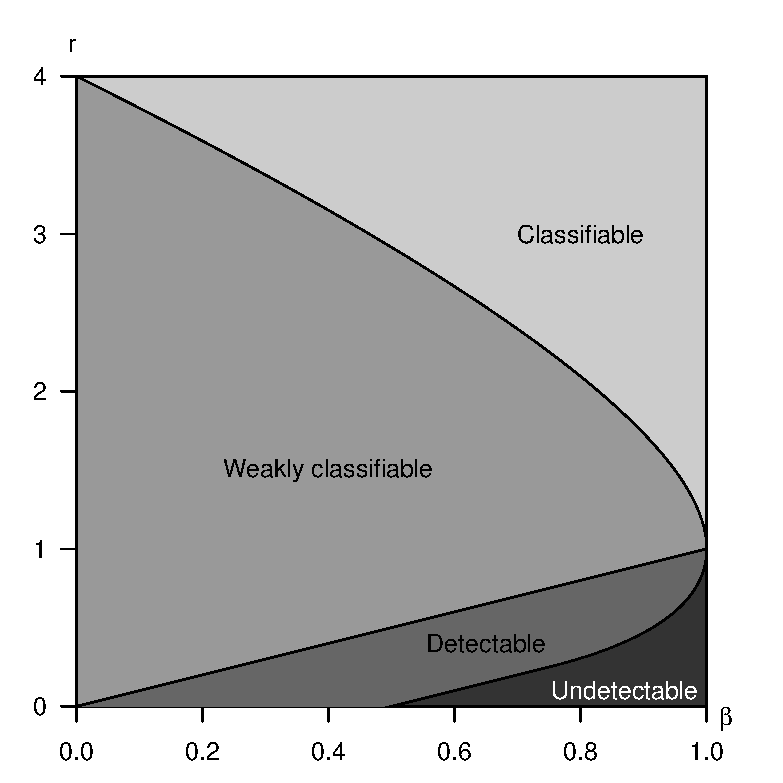
\includegraphics[width=0.45\textwidth]{./figures/phase_diagram_Gaussian_no_dashed_area.eps}
%       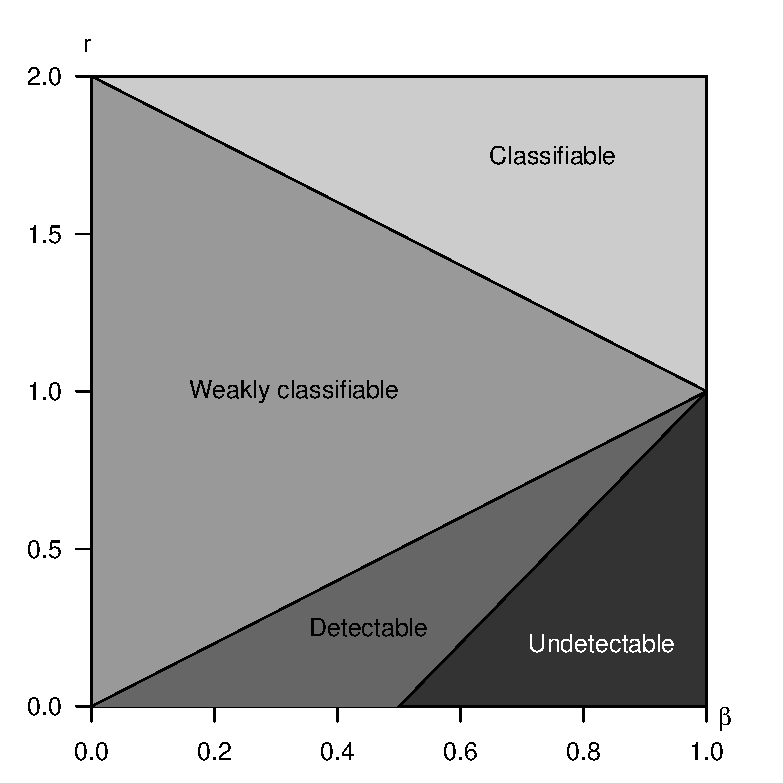
\includegraphics[width=0.45\textwidth]{./figures/phase_diagram_double_exponential.eps}
%       \caption{The phase diagrams of the detection, weak classification, and strong classification boundaries against sparse alternatives under Gaussian (left) and Laplace distributed (right) errors. Here $\beta$ and ${r}$ parametrize the signal sparsity and the lower and upper bounds of the signal sizes, respectively. 
%       The signal detection problem can be answered perfectly (asymptotically) inside the \emph{Detectable} region; false discovery proportion and non-discovery proportion can be made to vanish in the \emph{Weakly classifiable} region. We study in this paper the strong classification boundary, above which the support recovery can be achieved \emph{exactly} in the \emph{Classifiable} region $\{(\beta, {r}):{r}>g(\beta)\}$. 
%       In a large class of dependence structures characterized by URS, when signal sizes fall below the strong classification boundary \eqref{eq:strong-classification-boundary}, i.e. $\{(\beta, {r}):{r}<g(\beta)\}$, no thresholding procedure succeeds in the exact support recovery problem. }
%       \label{fig:phase}
% \end{figure}


\medskip
The phase transition phenomena for two additional classes of error distributions with either heavier or lighter tails than the AGG distributions will be described in Section \ref{suppsec:other-boundaries}.

\medskip
To conclude this summary, we emphasize that the sharp phase transition results established in this chapter apply only to
the general class of thresholding procedures.  In Chapter \ref{chap:optimality}, we characterize the finite-sample Bayes optimal support estimation procedures.
It will turn out that in many cases the optimal procedures are in fact thresholding procedures.  This will lead to complete phase transition
results valid for all types of support estimators, for certain classes of error models. In general, however, thresholding procedures
can be sub-optimal.  This has only recently been noticed by the statistical community in the case when the errors have heavy (regularly-varying) tails. 
\citet{arias2019detection} discussed the phenomenon in approximate support recovery problems.  In this case, we also demonstrate the absence 
of a phase transition phenomenon in exact support recovery by thresholding, in Section \ref{suppsec:heavy-tailed}. 


% In this sense, for $\nu\ge 1$ our results are rather complete.  We note here that our focus is not on minimax analysis of the support recovery problem, where a large class of distributional and dependence structures are considered.  
% In some sense, the worst case scenario (see also \cite{butucea2018variable}) is when the errors are independent.  
% In contrast, we establish the phase-transition phenomenon, for fixed but very general dependence conditions characterized by the URS property.


%We show that when the error-distribution $F$ is log-concave, then the thresholding procedures are optimal (for independent errors).  Therefore, in this regime the {\em strong classification boundary} $g$ is universal.  
%That is, if $r<g(\beta)$, no estimator can achieve perfect support recovery as $p\to\infty$. 
% \fbox{maybe skip the next sentence} 
% In fact, going beyond the class of rapidly varying distributions, (e.g., for heavy Pareto-type tails) the support recovery problem is fundamentally different and there may no longer be a phase-transition phenomenon.


%\section{Exact support recovery under AGG errors}
%\label{sec:boundary}

% We present the sufficient conditions for asymptotic exact support recovery in Section \ref{subsec:sufficient}.
% The study of maxima plays a central part in the study of support recovery problems.
% We present the key concepts regarding the behavior of the maxima, and in particular, the concentration of maxima phenomena, in Sections \ref{subsec:RS} and \ref{subsec:URS}. 
% These concepts enable to state a partial converse in Section \ref{subsec:necessary}.


\section{Sufficient conditions for exact support recovery}
\label{subsec:sufficient}

Following \citet*{butucea2018variable}, we define the parameter space for the signals $\mu$ as
\begin{align} \label{eq:minimax-signal-config-over}
    \Theta_p^+(\beta, \underline{r}) &= \{\mu\in\mathbb{R}^p:\;\text{there exists a set }S_p\subseteq\{1,\ldots,p\}\;\text{ such that }|S_p|\le\lfloor p^{1-\beta}\rfloor, \nonumber \\
    &\quad\quad\mu(i)\ge (\nu\underline{r}\log{p})^{1/\nu}\;\text{for all }i\in S_p,\;\text{and }\mu(i)=0\;\text{for all }i\not\in S_p\}.
\end{align}
Our first result states that, when $F\in \text{AGG}(\nu)$ with $\nu>0$, regardless of the error dependence structure, (asymptotic) perfect support recovery is achieved by applying Bonferroni's procedure with appropriately calibrated FWER, as long as the minimum signal size $\underline{r}$ is above the strong classification boundary \eqref{eq:strong-classification-boundary}.

\begin{theorem} \label{thm:sufficient}
Let the errors have common marginal distribution $F\in \text{AGG}(\nu)$ with $\nu>0$.
Let $\widehat{S}_p$ be the Bonferroni's procedure \eqref{eq:Bonferroni-procedure} with vanishing FWER $\alpha = \alpha(p) \to 0$, such that %\fbox{slower than any polynomial}
$\alpha p^\delta\to \infty$ for every $\delta>0$.
If
\begin{equation} \label{eq:signal-above-boundary}
    \underline{r} > f_{\mathrm{E}}(\beta) = (1 + (1 - \beta)^{1/\nu})^\nu,
\end{equation}
then we have
\begin{equation} \label{eq:exact-supporot-recovery}
    \lim_{p\to\infty}\sup_{\mu\in\Theta_p^+(\beta, \underline{r})} \P[\widehat{S}_p \neq S_p] = 0.
\end{equation}
\end{theorem}
\begin{proof}%[Proof of Theorem \ref{thm:sufficient}]
Throughout the proof, the dependence on $p$ will be suppressed to simplify notations when such omissions do not lead to ambiguity.

Under the $\text{AGG}(\nu)$ model, it is easy to see from equation \eqref{eq:AGG-quantiles} that the thresholds in Bonferroni's procedure are 
\begin{equation}\label{e:AGG-threshold}
t_p = F^{\leftarrow}(1 - \alpha/p) = (\nu\log{(p/\alpha)})^{1/\nu}(1+o(1)).
\end{equation}
It is known that Bonferroni's procedure $\widehat{S}_p = \left\{i:x(i)>t_p\right\}$ controls the FWER.  Indeed,
\begin{align} \label{eq:Bonferroni-FWER-control}
    \P\left[\widehat{S} \subseteq S\right] 
        &= 1 - \P\left[\max_{i\in S^c}x(i) > t_p\right] = 1 - \P\left[\max_{i\in S^c}\epsilon(i) > t_p\right]\nonumber \\
      % \ge 1 - \P\left[\max_{i\in\{1,\ldots,p\}}\epsilon(i) > t_p\right] \nonumber \\
        &\ge 1 - \sum_{i=1}^{p}\P\left[\epsilon(i)>t_p\right] \ge 1 - \alpha(p) \to 1,
\end{align}
where we used the union bound in the first inequality. 
Notice that the lower bound \eqref{eq:Bonferroni-FWER-control} is independent of the parameter $\mu$ (as well as the dependence structures), and hence holds uniformly over the parameter space, i.e.,
\begin{equation} \label{eq:exact-supporot-recovery-FWER}
    \lim_{p\to\infty}\inf_{\mu\in\Theta_p^+(\beta, \underline{r})} P[\widehat{S}_p \subseteq S_p] = 1.
\end{equation}


On the other hand, for the probability of no missed detection, we have:
\begin{equation*}
    \P\left[\widehat{S} \supseteq S\right] 
        = \P\left[\min_{i\in S}x(i) > t_p\right]
        = \P\left[\min_{i\in S}x(i) - (\nu\underline{r}\log p)^{1/\nu} > t_p - (\nu\underline{r}\log p)^{1/\nu} \right].
\end{equation*}
Since the signal sizes are no smaller than $(\nu\underline{r}\log p)^{1/\nu}$, we have
\begin{equation*}
    x(i) - \left(\nu\underline{r}\log{p}\right)^{1/\nu} \ge \epsilon(i), \quad \text{for all }i\in S,
\end{equation*}
and hence we obtain
\begin{equation} \label{eq:sufficient-proof-eq1}
    \P\left[\widehat{S} \supseteq S\right] \ge 
    \P\left[\min_{i\in S}\epsilon(i) > (\nu\log{(p/\alpha)})^{1/\nu}(1+o(1)) - (\nu\underline{r}\log p)^{1/\nu} \right],
\end{equation}
where we plugged in the expression for $t_p$ in \eqref{e:AGG-threshold}.
Now, since the minimum signal size is bounded below by $\underline{r} > \left(1 + (1-\beta)^{1/\nu}\right)^\nu$, we have $\underline{r}^{1/\nu}-(1-\beta)^{1/\nu}>1$, and so we can pick a $\delta > 0$ such that 
\begin{equation} \label{eq:choice-of-delta}
    \delta < \left(\underline{r}^{1/\nu} - (1-\beta)^{1/\nu}\right)^\nu - 1.
\end{equation}
Since by assumption, for all $\delta>0$, we have $p^{-\delta} = o\left(\alpha(p)\right)$, there is an
$M=M(\delta)$ such that $p/\alpha(p) < p^{1+\delta}$ for all $p\ge M$. Thus, from \eqref{eq:sufficient-proof-eq1}, we further conclude that for $p\ge M$ we have
\begin{align}
    \P\Big[\widehat{S} \supseteq S\Big]
      &\ge \P\Big[\min_{i\in S}\epsilon(i) > \left((1+\delta)\nu\log{p}\right)^{1/\nu}(1+o(1)) - (\nu\underline{r}\log p)^{1/\nu} \Big] \nonumber \\
      &= \P\Big[\max_{i\in S}\left(-\epsilon(i)\right) < \underbrace{\left(\underline{r}^{1/\nu} - (1+\delta)^{1/\nu}\right)(\nu\log{p})^{1/\nu}(1+o(1))}_{=:\text{A}} \Big] \nonumber \\
      &\ge 1 - \lfloor p^{1-\beta} \rfloor \times \overline{F}_-(\text{A}), \label{eq:sufficient-proof-eq2}
      % &\ge 1 - |S|\times\P\Big[(-\epsilon(1)) \ge \left(\underline{r}^{1/\nu} - (1+\delta)^{1/\nu}\right)(\nu\log{p})^{1/\nu}(1+o(1)) \Big] 
\end{align}
where $\overline{F}_-(x) = \P[-\epsilon(i)>x]$ is the survival function of the $(-\epsilon(i))$'s.
Notice that \eqref{eq:sufficient-proof-eq2} follows from the union bound and the assumption that ${|S_p|}\le{\lfloor p^{1-\beta}\rfloor}$. 
Therefore, the lower bound does not depend on $\mu$ (nor on the error dependence structure), and holds uniformly in the parameter space. In turn, we obtain 
\begin{equation} \label{eq:exact-supporot-recovery-FWNR}
    \inf_{\mu\in\Theta_p^+(\beta, \underline{r})} \P[\widehat{S}_p \supseteq S_p] \ge 1 - \lfloor p^{1-\beta} \rfloor \times \overline{F}_-(\text{A}).
\end{equation}

If $\beta=1$, we conclude that the right-hand-side of \eqref{eq:exact-supporot-recovery-FWNR} 
converges to $1$, since $\text{A}\to+\infty$.

Let now $\beta\in (0,1)$ and $u_p^- :=  F_-^{\leftarrow}(1-1/p)$. 
The fact that $p\overline{F}_-(u_p^-) \le 1$, implies
\begin{equation}
    \lfloor p^{1-\beta} \rfloor \times \overline{F}_-(\text{A}) \le 
    \frac{\overline{F}_-\left(\text{B}\times{u_{\lfloor p^{1-\beta}\rfloor}^-}\right)} {\overline{F}_-\left({u_{\lfloor p^{1-\beta}\rfloor}^-}\right)} \label{eq:sufficient-proof-eq3}
    % \P\Big[\frac{\max_{i\in S}(-\epsilon(i))}{u_{|S|}}\frac{u_{|S|}}{u_{\lfloor p^{1-\beta}\rfloor}} < \underbrace{\frac{\underline{r}^{1/\nu} - (1+\delta)^{1/\nu}}{(1-\beta)^{1/\nu}}\left(1+o(1)\right)}_{=:\text{B}}\Big], \label{eq:exact-supporot-recovery-FWNR}
\end{equation}
where $\text{B} := {\text{A}}/{u_{\lfloor p^{1-\beta}\rfloor}^-}$.

Notice that by assumption, the $-\epsilon(i)$'s are also 
AGG$(\nu)$ distributed and by Proposition \ref{prop:quantile}, 
$u_p^{-}:= F_-^{\leftarrow}(1-1/p) \sim (\nu \log(p))^{1/\nu}$,
as $p\to\infty$. Therefore, we have
\begin{equation} \label{eq:sufficient-proof-eq4}
    u_{\lfloor p^{1-\beta}\rfloor}^- \sim \left(\nu(1-\beta)\log{p}\right)^{1/\nu}
\end{equation}
and 
\begin{equation*}
\text{B} = \frac{\text{A}}{u_{\lfloor p^{1-\beta}\rfloor}^-}
= \frac{\underline{r}^{1/\nu} - (1+\delta)^{1/\nu}}{(1-\beta)^{1/\nu}}\left(1+o(1)\right) \to c>1
\end{equation*}
as $p\to\infty$, by our choice of $\delta$ in \eqref{eq:choice-of-delta}.

Finally, since the distribution $F_-$ has \emph{rapidly varying} tails (by Definition \ref{def:rapid-variation} and Example \ref{exmp:AGG}), applying Proposition \ref{prop:rapid-varying-tails}, we conclude that \eqref{eq:sufficient-proof-eq3} vanishes. Consequently, the lower bound on the right-hand-side of \eqref{eq:exact-supporot-recovery-FWNR} converges to 1.
This, combined with \eqref{eq:exact-supporot-recovery-FWER}, entails {$\lim_{p\to\infty} \inf_{\mu\in\Theta_p^+(\beta, \underline{r})} \P[\widehat{S}_p = S_p]= 1$, and hence the desired conclusion \eqref{eq:exact-supporot-recovery}, which completes the proof}.
\end{proof}

\medskip
We end this section with several comments and applications of Theorem \ref{thm:sufficient}.
\begin{corollary}[Classes of procedures attaining the boundary]
\label{cor:FWER-controlling_procedures}  
Relation \eqref{eq:exact-supporot-recovery} holds for any FWER-controlling procedure that is strictly more powerful than Bonferroni's procedure. 
This includes Holm's procedure \citep*{holm1979simple}, and in the case of independent errors, Hochberg's procedure \citep*{hochberg1988sharper}, and the {\v{S}}id{\'a}k procedure \citep*{vsidak1967rectangular}.
\end{corollary}

\begin{example} \label{exmp:FWER-controlling_procedures}
Under Gaussian errors, the particular choice of the thresholding at $t_p = \sqrt{2\log{p}}$ in \eqref{eq:Bonferroni-procedure} corresponds to a Bonferroni's procedure with FWER decreasing at a rate of ${\cal O}((\log{p})^{-1/2})$, and hence Theorem \ref{thm:sufficient} applies. 
By Corollary \ref{cor:FWER-controlling_procedures}, Holm's procedure --- and when the errors are independent, the {\v{S}}id{\'a}k, and Hochberg procedures --- with FWER controlled at $(\log{p})^{-1/2}$ all achieve perfect support recovery provided that $\underline{r}>f_{\mathrm{E}}(\beta)$.

\begin{proof}[Example \ref{exmp:FWER-controlling_procedures}]
By the Mill's ratio for the standard Gaussian distribution,
$$
\frac{t_p \P\left[Z>t_p\right]}{\phi(t_p)} \to 1,\quad \text{as}\quad t_p\to\infty,
$$
where $Z\sim \text{N}(0,1)$. 
Using the expression for $t_p = \sqrt{2\log{p}}$, we have
$$
p \;\P\left[Z>t_p\right] \sim \sqrt{2\pi}^{-1}\left(2\log{p}\right)^{-1/2} \to 0,
$$
as desired. The rest of the claims follow from Corollary \ref{cor:FWER-controlling_procedures}.
\end{proof}
\end{example}


The statements in Theorem \ref{thm:sufficient} can be strengthened, to prepare us for a minimax result given in Section \ref{sec:minimax} below.

\begin{remark} \label{rmk:sufficient-strengthened}
In the proof of Theorem \ref{thm:sufficient}, both \eqref{eq:Bonferroni-FWER-control} and \eqref{eq:sufficient-proof-eq2} hold uniformly over all error dependence structures.
Therefore, \eqref{eq:exact-supporot-recovery-FWER} and \eqref{eq:exact-supporot-recovery-FWNR} may be strengthened to yield
\begin{equation} \label{eq:exact-supporot-recovery-strengthened}
    \lim_{p\to\infty}\sup_{\substack{\mu\in\Theta_p^+(\beta, \underline{r})\\ {\cal E}\in D(F)}} P[\widehat{S}_p \neq S_p] = 0,
\end{equation}
for $\underline{r} > f_{\mathrm{E}}(\beta)$, where $D(F)$ is the collection of all arrays with common marginal $F$, i.e., 
\begin{equation} \label{eq:common-marginal-distribution}
    D(F)=\{{\cal E}=(\epsilon_p(i))_p:\;\epsilon_p(i)\sim F\;\text{for all }i=1,\ldots,p, \text{and}\; p=1,2,\ldots\}.
\end{equation}
\end{remark}

\begin{remark}
We emphasize that Theorem \ref{thm:sufficient} holds for errors with \emph{arbitrary} dependence structures. 
Intuitively, this is because the maxima of the errors grow at their fastest in the case of independence (recall Remark \ref{rem:iid-max}). 
Formally, the light-tailed nature of the error distribution allowed us to obtain sharp tail estimates via simple union bounds, 
valid under arbitrary dependence.
% Formally, this result stems from the fact that maxima of distributions with \emph{rapidly varying tails} (Definition \ref{def:rapid-variation}) can be bounded from above using quantiles of their marginal distribution, under arbitrary dependence.
\end{remark}
% We turn next to the study of maxima and present the tools used in the proof of Theorem \ref{thm:sufficient}.
% Thus, the support recovery problem is hardest under independent errors.
% The relationship between dependence and the behavior of maxima is discussed next in Section \ref{sec:URS}, where we will see that the phase-transition phenomenon is not limited to just the AGG models and independent errors; such phenomenon exists for all error models with rapidly varying tails, and under a surprisingly large class of dependent structures.
% On the other hand, the converse of Theorem \ref{thm:sufficient} will need an (extremely mild) assumption on error dependence structures.


\section{Dependence and uniform relative stability}
\label{subsec:URS}

An important ingredient needed for a converse of Theorem \ref{thm:sufficient} is an appropriate characterization of the error dependence structure under which the strong classification boundary \eqref{eq:strong-classification-boundary} is tight.
The notion of \emph{uniform relative stability} turns out to be the key.
% in characterizing such dependence structures when studying the behavior of maxima of dependent light-tailed sequences.

\begin{definition}[Uniform Relative Stability] \label{def:URS}
Under the notations established in Definition \ref{def:RS}, the triangular array ${\cal E}$ is said to have uniform relatively stable (URS) maxima if for \emph{every} sequence of subsets $S_p\subseteq\{1,\ldots,p\}$ such that $|S_p| \to \infty$, we have
\begin{equation} \label{eq:URS-condition}
    \frac{1}{u_{|S_p|}} M_{S_p} := \frac{1}{u_{|S_p|}} \max_{i\in S_p} \epsilon_p(i) \xrightarrow{\P} 1,
\end{equation}
as $p\to\infty$, where $u_q,\ q\in \{1,\ldots,p\}$ is the generalized quantile in \eqref{eq:quantiles}.
The collection of arrays ${\cal E} = \{ \epsilon_p(i) \}$ with URS maxima is 
denoted $U(F)$.
\end{definition}

Uniform relative stability is, as its name suggests, a stronger requirement on dependence than relative stability (recall Definition \ref{def:RS}). 
Proposition \ref{prop:rapid-varying-tails} states that an array with iid components sharing a marginal distribution $F$ with rapidly varying tails (Definition  \ref{def:rapid-variation}) has relatively stable maxima; it is easy to see that URS also follows, by independence of the entries.

\begin{corollary} \label{cor:AGG-is-URS}
An independent array ${\cal E}$ with common marginals $F\in\text{AGG}(\nu)$, $\nu>0$, is URS; in this case, URS holds with $u_{|S_p|} \sim \left(\nu\log{|S_p|}\right)^{1/\nu}$.
\end{corollary}

On the other hand, RS and URS hold under much broader dependence structures than just 
independent errors. 
These conditions are extremely mild and can be shown to hold for many classes of error models.  
In Chapter \ref{chap:URS}, we will focus extensively on the Gaussian case, which is of great interest in applications and is rather challenging. 
We will provide simple necessary and sufficient condition for uniform relative stability in terms of the covariance structures.

The relative stability concepts are important because they characterize the dependence structures under which the maxima of error sequences {\em concentrate} around the quantiles \eqref{eq:quantiles} in the sense of \eqref{eq:RS-condition}.
This concentration of maxima phenomena, in turn, is the key to establishing the necessary conditions of the phase transition results in support recovery problems.

% The importance of the URS dependence class in statistics is seen in the study of support recovery problems, discussed next.

\section{Necessary conditions for exact support recovery}
\label{subsec:necessary}

With the preparations from Section \ref{subsec:URS}, we are ready to state the necessary conditions for exact support recovery \eqref{eq:exact-recovery} by thresholding procedures. 
It turns out that the strong classification boundary \eqref{eq:strong-classification-boundary} is tight, under the general dependence structure characterized by URS (Definition \ref{def:URS}).

Formally, we define the parameter space for the signals $\mu$ to be
\begin{align} \label{eq:minimax-signal-config-under}
    \Theta_p^-(\beta, \overline{r}) &= \{\mu\in\mathbb{R}^p:\;\text{there exists a set }S_p\subseteq\{1,\ldots,p\}\;\text{ such that }|S_p|=\lfloor p^{1-\beta}\rfloor, \nonumber \\
    &\quad\quad0<\mu(i)\le(\nu\overline{r}\log{p})^{1/\nu}\;\text{for all }i\in S_p,\;\text{and }\mu(i)=0\;\text{for all }i\not\in S_p\}.
\end{align}


\begin{theorem} \label{thm:necessary}
    Let ${\cal E}$ be a triangular array with common $\text{AGG}(\nu)$ marginal $F$, $\nu > 0$.
    % Let the signal $\mu$ have $|S_p| = \lfloor p^{(1-\beta)} \rfloor$ non-zero entries where $\beta\in(0,1]$, where the signal sizes $\mu(i)$, $i\in S_p$ are at most $\overline{\Delta} = \left(\nu\overline{r}\log p\right)^{1/\nu}$.
    % and the signals $\mu$ have $s=|S|=\lfloor p^{1-\beta}\rfloor$ be as described in Theorem \ref{thm:sufficient}. 
    Assume further that the errors ${\cal E}$ have uniform relatively stable maxima and minima, i.e., ${\cal E}\in U(F)$, and $(-{\cal E}) = \{-\epsilon_{p}(i)\} \in U(F)$.
    If 
    \begin{equation} \label{eq:signal-below-boundary}
        \overline{r} < f_{\mathrm{E}}(\beta) = \left(1+(1-\beta)^{1/\nu}\right)^\nu,
    \end{equation}
    then
    \begin{equation} \label{eq:classification-impossible-dependent}
        \lim_{p\to\infty} \inf_{\widehat{S}_p\in{\cal T}} \inf_{\mu\in{\Theta_p^-(\beta, \overline{r})}} \P[\widehat{S}_p \neq S_p] = 1,
    \end{equation}
    where ${\cal T}$ is the class of all thresholding procedures \eqref{eq:thresholding-procedure}.
\end{theorem}
\begin{proof} %[Proof of Theorem \ref{thm:necessary}]
To avoid cumbersome double subscript notations, we will sometimes suppress dependence on $p$ of the set sequences $\widehat{S}_p$ and $S_p$ in the proof.

Since the estimator $\widehat{S}_p = \{x(i) \ge t_p(x)\}$ is thresholding, exact support recovery takes place if and only if the threshold separates the signals and null part, i.e.,
\begin{equation*}
    \P[\widehat{S}_p = S_p] 
    = \P\left[\max_{i\in S^c}x(i) < t_p(x) \le \min_{i\in S}x(i)\right]
    \le \P\left[\max_{i\in S^c}x(i) < \min_{i\in S}x(i)\right].
\end{equation*}
Since the right-hand-side does not depend on the procedure $\widehat{S}_p$, we also have
\begin{equation} \label{eq:classification-possible-dependent-proof-1}
    \sup_{\widehat{S}_p\in{\cal T}} \P[\widehat{S}_p = S_p] 
    \le \P\left[\max_{i\in S^c}x(i) < \min_{i\in S}x(i)\right]
    \le \P\left[{\max_{i\in S^c}\epsilon(i)} < {\overline{\Delta} + \min_{i\in S}\epsilon(i)}\right],
\end{equation}
where we used the assumption that the signal sizes are no greater than $\overline{\Delta}$.
Let $S^* = S_p^*$ be a sequence of support sets that maximize the right-hand-side of \eqref{eq:classification-possible-dependent-proof-1}, i.e., let
$$
S_p^* = \argmax_{S\subseteq\{1,\ldots,p\}:|S| = \lfloor p^{1-\beta}\rfloor} \P\left[{\max_{i\in S^c}\epsilon(i)} < {\overline{\Delta} + \min_{i\in S}\epsilon(i)}\right],
$$
where ties can be broken lexicographically if multiple maximizers exist.
Then,
% Since there is only a finite number support set $S$ in $\mathcal{S} = \left\{S\subseteq\{1,\ldots,p\};|S|=\lfloor p^{1-\beta}\rfloor\right\}$, we can bound \eqref{eq:classification-possible-dependent-proof-1} from above uniformly over $\mathcal{S}$ as well.
% In particular, let 
% $$
% S^* = S^*_p \in \argmax_{S\in{\mathcal{S}}}\P\left[{\max_{i\in S^c}\epsilon(i)} < {\overline{\Delta} + \min_{i\in S}\epsilon(i)}\right],
% $$
we obtain the following bound which only depends on $\overline{r}$ and the distribution of ${\cal E}$,
\begin{align}
    \sup_{\widehat{S}_p\in{\cal T}} \sup_{\mu\in\Theta^-_p(\beta,\overline{r})} \P[\widehat{S}_p = S_p] 
    % \P\left[{\max_{i\in S^c}\epsilon(i)} < {\overline{\Delta} + \min_{i\in S}\epsilon(i)}\right]
    &\le \P\left[{\max_{i\in S^{*c}}\epsilon(i)} < {\overline{\Delta} + \min_{i\in S^*}\epsilon(i)}\right] \nonumber \\
% \end{align}
% \begin{align}
% \P\left[\max_{i\in S^c}x(i) < \min_{i\in S}x(i)\right]  
%   &= \P\left[\frac{\max_{i\in S^c}x(i)}{u_p} < \frac{\min_{i\in S}x(i)}{u_p}\right] \nonumber \\
%   &\le  \P\left[\frac{\max_{i\in S^c}\epsilon(i)}{u_p} < \frac{\min_{i\in S}\overline{\Delta} + \epsilon(i)}{u_p}\right] \nonumber \\
  &= \P\left[ \frac{M_{S^{*c}}}{u_p} < \frac{\overline{\Delta} - m_{S^*}}{u_p} \right], \label{eq:classification-possible-dependent-proof-2}
\end{align}
where $M_{S^{*c}} = \max_{i\in S^{*c}}\epsilon(i)$ and $m_{S^*} = \max_{i\in S^*}\left(-\epsilon(i)\right)$.
Since the error arrays ${\cal E}$ and $(-{\cal E})$ are URS by assumption, using the expression for the AGG quantiles \eqref{eq:AGG-quantiles}, we have
\begin{equation} \label{eq:classification-possible-dependent-proof-3}
    \frac{M_{S^{*c}}}{u_p} = \frac{M_{S^{*c}}}{u_{|S^{*c}|}} \frac{u_{|S^{*c}|}}{u_p} \xrightarrow{\P} 1,
\quad \text{and} \quad
\frac{m_{S^*}}{u_p} = \frac{m_{S^*}}{u_{|S^*|}} \frac{u_{|S^*|}}{u_p} \xrightarrow{\P} (1-\beta)^{1/\nu},
\end{equation}
so that the two random terms in probability \eqref{eq:classification-possible-dependent-proof-2} converge to constants.
Notice that the second relation in \eqref{eq:classification-possible-dependent-proof-3} holds by URS for any $\beta\in(0,1)$; when $\beta=1$, the relation holds since ${u_{|S^*|}}/{u_p}$ vanishes while $\{{m_{S^*}}/{u_{|S^*|}}\}$ is tight.

Since signal sizes are bounded above by $\overline{r} < \left(1 + (1-\beta)^{1/\nu}\right)^{\nu}$, we can write $\overline{r}^{1/\nu} = 1 + (1-\beta)^{1/\nu} - d$ for some $d > 0$. By our parametrization of $\overline{\Delta}$, we have
\begin{equation} \label{eq:classification-possible-dependent-proof-4}
    \frac{\overline{\Delta}}{u_p} = \left(1+(1-\beta)^{1/\nu}-d\right)(1+o(1)).
\end{equation}
Combining \eqref{eq:classification-possible-dependent-proof-3} and \eqref{eq:classification-possible-dependent-proof-4}, we conclude that the right-hand-side of the probability \eqref{eq:classification-possible-dependent-proof-2} converges in probability to a constant strictly less than 1, that is, 
\begin{equation}
    \frac{\overline{\Delta} - m_S}{u_p} \xrightarrow{\P} 1 - d,
\end{equation}
while ${M_{S^{*c}}}/{u_p} \xrightarrow{\P} 1$.
Therefore, the probability in \eqref{eq:classification-possible-dependent-proof-2} must go to 0.
\end{proof}


% We comment on some consequences of the theorem, before presenting its proof.
We end this section with several remarks on the scope and consequences
of our results. Our first comment is on the signal sizes, and in particular, the gap 
between the sufficient conditions (Theorem \ref{thm:sufficient}) and the necessary 
conditions (Theorem \ref{thm:necessary}).

\begin{remark}[Minding the gap] \label{rmk:gap-between-sufficient-necessary}
The sufficient condition in Theorem \ref{thm:sufficient} requires that \emph{all} signals be larger than the strong classification boundary $f_{\mathrm{E}}(\beta)$ in order to achieve exact support recovery \eqref{eq:exact-recovery}, while Theorem \ref{thm:necessary} states that exact support recovery fails (in the sense of \eqref{eq:exact-recovery-failure}) when \emph{all} signal sizes are below the boundary --- the two conditions are \emph{not} complements of each other.
This gap between the sufficient and necessary conditions on signal sizes, however, may be difficult to bridge.
Indeed, in general, when signal sizes straddle the boundary $f_{\mathrm{E}}(\beta)$, either outcome is possible, as we demonstrate in 
Example \ref{exmp:signals-straddling-the-boundary} below.
\end{remark}

\begin{example}[Signals straddling the boundary]
\label{exmp:signals-straddling-the-boundary}
Let the signal $\mu$ have $|S_p| = \lfloor p^{(1-\beta)} \rfloor$ non-zero entries, composed of two disjoint sets $S_p = S_p^{(1)}\cup S_p^{(2)}$.
Let also the magnitude of the signals be equal within the two sets, i.e., $\mu(i)=\sqrt{2r^{(k)}\log{p}}$ if $i\in S_p^{(k)}$ for some constants $r^{(k)} > 0$ for $k=1,2$.
For simplicity, assume that the errors are iid standard Gaussians.

Consider two scenarios
\begin{enumerate}
    \item $r^{(1)} = (1+\delta)f_{\mathrm{E}}(\beta)$, $r^{(2)} = (1+\delta)$ with $|S_p^{(1)}|=|S_p|-1$, $|S_p^{(2)}|=1$, 
    \item $r^{(1)} = (1+\delta)f_{\mathrm{E}}(\beta)$, $r^{(2)} = (1-\delta)f_{\mathrm{E}}(\beta)$ with $|S_p^{(1)}|=\lfloor|S_p|/2\rfloor$, $|S_p^{(2)}|=|S_p| - |S_p^{(1)}|$.
\end{enumerate}
for some constants $0<\delta<1-\beta<1$. 
In both cases, signals in $S_p^{(1)}$ (respectively, $S_p^{(2)}$) are above (respectively, below) the strong classification boundary \eqref{eq:strong-classification-boundary}.
However, in the first scenario, we have $\mathbb{P}[\widehat{S}^{\text{Bonf}}_p=S_p]\to 1$ where $\widehat{S}^{\text{Bonf}}_p$ is the Bonferroni's procedure described in Theorem \ref{thm:sufficient}, 
while in the second scenario, we have $\mathbb{P}[\widehat{S}_p=S_p]\to 0$ for \emph{all} thresholding procedures $\widehat{S}_p$.

\begin{proof}[Example \ref{exmp:signals-straddling-the-boundary}]
In the first scenario, signal sizes in $S^{(1)}_p$ are by definition above the strong classification boundary \eqref{eq:strong-classification-boundary}.
The signal in $S^{(2)}_p$ has size parameter $1+\delta<2-\beta<(1+\sqrt{1-\beta})^2$, and therefore falls below the boundary.

It remains to show that $\mathbb{P}[\widehat{S}^{\text{Bonf}}_p=S_p]\to 1$.
To do so, we define two new arrays 
$$
{\cal Y}^{(k)} = \{y^{(k)}_p(j),\;j=1,2,\ldots,p\},\quad k\in\{1,2\}_p,
$$
where $y^{(k)}_p(j)=x_p(j)$ if $j\not\in S^{(k)}_p$, and $y^{(k)}_p(j)=\widetilde{\epsilon}_p(j)$ if $j\in S^{(k)}_p$, using an independent error array $\{\widetilde{\epsilon}_p(j),\;j=1,\ldots,p\}$ with iid standard Gaussian elements.
That is, we replace the elements in $S^{(1)}_p$ and $S^{(2)}_p$ with iid standard Gaussian noise.
Notice both arrays ${\cal Y}^{(1)}$ and ${\cal Y}^{(2)}$ satisfy the conditions in Theorem \ref{thm:sufficient} (with sparsity parameter equal to $\beta$ and $1$, respectively). 
Hence, we have
$$
\P[\widehat{S}^{\text{Bonf}}_p\subseteq S_p] 
= \P\left[\max_{j\in S^c}x(j) \le t_p\right]
\le \P\left[\max_{j\in S^c}y^{(1)}(j) \le t_p\right] \to 0,
$$
and 
\begin{align*}
    \P[\widehat{S}^{\text{Bonf}}_p\supseteq S_p]
    &= \P\left[\min_{j\in S}x(j) > t_p\right] 
    \ge 1 - \P\left[\min_{j\in S^{(1)}}x(j) \le t_p\right] - \P\left[\min_{j\in S^{(2)}}x(j) \le t_p\right] \\
    &\ge 1 - \P\left[\min_{j\in S^{(1)}}y^{(2)}_p(j) \le t_p\right] - \P\left[\min_{j\in S^{(2)}}y^{(1)}_p(j) \le t_p\right] 
    \to 1,
\end{align*}
where $t_p$ is the threshold in Bonferroni's procedure. The conclusion follows.
% only need to show $\mathbb{P}[S^{(2)}_p\subseteq\widehat{S}^{\text{Bonf}}_p]\to 1$.

In the second scenario, the signal sizes in $S^{(2)}$ by definition fall below the strong classification boundary \eqref{eq:strong-classification-boundary}.
To see that no thresholding procedure succeeds, we adapt the proof of Theorem \ref{thm:necessary}.
In particular, we obtain
$$
    \P[\widehat{S}_p = S_p] 
    \le \P\left[\max_{j\in S^c}x(j) \le t_p < \min_{j\in S}x(j)\right]
    \le \P\left[\max_{j\in S^c}x(j) < \min_{j\in S^{(2)}}x(j)\right].
$$
By the assumption that signals in $S^{(2)}$ have size parameter $(1-\delta)f_{\mathrm{E}}(\beta)$, we have
\begin{equation}
\P\left[\max_{j\in S^c}x(j) < \min_{j\in S^{(2)}}x(j)\right]
= \P\left[ \frac{M_{S^{c}}}{u_p} < \frac{\sqrt{2(1-\delta)f_{\mathrm{E}}(\beta)\log{p}} - m_{S^{(2)}}}{u_p}\right], 
\end{equation}
where $M_{S^{c}} = \max_{j\in S^{c}}\epsilon(j)$ and $m_{S^{(2)}} = \max_{j\in S^{(2)}}\left(-\epsilon(j)\right)$.
The ratio on the left-hand-side of the inequality converges to 1 as in \eqref{eq:classification-possible-dependent-proof-3} in the main text, whereas the term on the right-hand-side
\begin{align*}
    \frac{\sqrt{2(1-\delta)f_{\mathrm{E}}(\beta)\log{p}} - m_{S^{(2)}}}{u_p} 
    &= \sqrt{(1-\delta)f_{\mathrm{E}}(\beta)} - \frac{m_{S^{(2)}}}{u_{|S^{(2)}|}} \frac{u_{|S^{(2)}|}}{u_p} \\
    &\xrightarrow{\P} \sqrt{(1-\delta)} + \sqrt{1-\beta}(\sqrt{(1-\delta)} - 1) < 1.
\end{align*}
where we used the URS of the error arrays, and that 
$$
u_{|S^{(2)}|} \sim \sqrt{2\log{(p^{1-\beta}/2)}} 
= \sqrt{2(({1-\beta})\log{p}-\log2)} \sim \sqrt{2({1-\beta})\log{p}}.
$$
to conclude the convergence in probability.
\end{proof}
\end{example}

Our second remark is on the restriction to thresholding procedures.
\begin{remark}
	we emphasize that the sharp phase transition result just established apply only to the general class of thresholding procedures. It is natural to ask if we have left out the other good procedures in this restriction.
	We will establish in Chapter \ref{chap:optimality} below that in many cases the optimal procedures are in fact thresholding procedures. In general, however, thresholding procedures can be sub-optimal, e.g., when the errors have heavy (regularly-varying) tails. 
	We will also demonstrate the absence of a phase transition phenomenon in exact support recovery by thresholding, in Supplement Section \ref{suppsec:heavy-tailed}. 
\end{remark}

Our final comment is on the interplay between thresholding procedures and the dependence class characterized by URS.
\begin{remark} \label{rmk:dependence-assumptions}
Paraphrasing Theorems \ref{thm:sufficient} and \ref{thm:necessary}: if we consider only thresholding procedures, then for a very large class of dependence structures, we cannot improve upon the Bonferroni procedure $\widehat{S}_p^{\text{Bonf}}$. 
Specifically, for all ${\cal E}\in U(F)$ and ${-\cal E}\in U(F)$, and for all $S_p\in {\cal S}$, where $\mathcal{S} = \left\{S\subseteq\{1,\ldots,p\};|S|=\lfloor p^{1-\beta}\rfloor\right\}$, we have
\begin{equation}
    \lim_{p\to\infty} \P[\widehat{S}_p^{\text{Bonf}}\neq S_p]
    = \begin{cases}
    \limsup_{p\to\infty} \inf_{\widehat{S}_p \in {\cal T}} \P[\widehat{S}_p\neq S_p] = 0, & \text{if}\quad \underline{r} > f_{\mathrm{E}}(\beta),\\
    \liminf_{p\to\infty} \inf_{\widehat{S}_p \in {\cal T}} \P[\widehat{S}_p\neq S_p] = 1, & \text{if}\quad \overline{r} < f_{\mathrm{E}}(\beta)\\
    \end{cases}
\end{equation}
where $\cal T$ is the set of all thresholding procedures \eqref{eq:thresholding-procedure}. 

Theorem \ref{thm:necessary} answers a question raised in \citet{butucea2018variable}.
In particular, the authors of \citep{butucea2018variable} commented that independent error is the  `least favorable model' in the problem of support recovery, and 
conjectured that the support recovery problem may be easier to solve under dependence, similar to how the problem of signal detection is easier under dependent 
errors \citep{hall2010innovated}. 
Surprisingly, our results here state that asymptotically, \emph{all} error dependence structures in the large URS class are equally difficult for \emph{thresholding procedures}. Therefore, the phase transition behavior is universal in the class of dependence structures characterized by URS.
%For more details, see also Section \ref{sec:minimax}.
\end{remark}

The restriction to the URS dependence class in Theorem \ref{thm:necessary} is \emph{not} an assumption of convenience. 
The dependence condition characterized by uniform relative stability is, in fact, one of the weakest in the literature.
We will characterize the class URS dependence class in Chapter \ref{chap:URS} below.


% \begin{remark}   {\color{blue} Here is an idea -- one could estimate the threshold robustly.  For example,
% suppose that we know that the support set is of size $\le p^{1-\beta_0}$, for some fixed $\beta_0\in(0,1)$.  Assume also (for simplicity) that the
% signals can only be positive.  Then, let
% $$
% T_p := x_{([p^{1-\beta_0}])},
% $$
% be the top $[p^{1-\beta_0}]$-th order statistic of the data.  Then, I believe, but I have not proved it that in the absence of signal
% $T_p/u_p \to 1$ in probability.  This should be easy to verify in the iid case and it is an {\bf open problem} in the general URS case. 
% Therefore, one can take the threshold to be:
% $$ t_p(\delta)  := T_p\times (1+\delta),$$ 
% where $\delta>0$ is something tiny (which can also be made to vanish slowly as $p\to\infty$.

% We know, from our theory that if a threshold estimator is to be able to recover the support, then all the signal entries should be 
% above $T_p$ (since we assume that the sparsity $\beta<\beta_0$).  Thus, it is plausible that in this case, the value of
% $T_p$ is unaffected by the signal and $T_p\sim u_p$ in probability.  Now, the factor $1+\delta$ makes the threshold $t_p$ just large enough for it to
% miss any false positives, and if $\delta>0$ is small, to capture all the signal, as $p\to\infty$.

% This idea can be easily checked with simulations to see how well it does in practice.  It is almost completely non-parametric!!! 
% What do you think?   If it ``works", should we include it? 
% }
% \end{remark}




\section{Dense signals}
\label{subsec:dense-signals}

We treat briefly the case of dense signals,
% In the revision of the initial manuscript, the associate editor pointed out the important issue of dense signals, 
where the size of the support set is proportional to the problem dimension, i.e. $s\sim cp$ for some constant $c\in(0,1)$.
We show that in this case, a phase-transition-type result still holds, independently of the value of $c$. 
Analogous to the set-up of Theorems \ref{thm:sufficient} and \ref{thm:necessary}, let
\begin{align} \label{eq:minimax-signal-config-over-dense}
    \Theta_p^{\mathrm{d}+}(c, \underline{r}) &= \{\mu\in\mathbb{R}^p:\;\text{there exists a set }S_p\subseteq\{1,\ldots,p\}\;\text{ such that }|S_p|\le\lfloor cp\rfloor, \nonumber \\
    &\quad\quad\mu(i)\ge (\nu\underline{r}\log{p})^{1/\nu}\;\text{for all }i\in S_p,\;\text{and }\mu(i)=0\;\text{for all }i\not\in S_p\},
\end{align}
where ``$\mathrm{d}$'' in the notation $\Theta_p^{\mathrm{d}+}$ stands for ``dense''. 
Similarly, define
\begin{align} \label{eq:minimax-signal-config-under-dense}
    \Theta_p^{\mathrm{d}-}(c, \overline{r}) &= \{\mu\in\mathbb{R}^p:\;\text{there exists a set }S_p\subseteq\{1,\ldots,p\}\;\text{ such that }|S_p|=\lfloor cp\rfloor, \nonumber \\
    &\quad\quad0<\mu(i)\le (\nu\overline{r}\log{p})^{1/\nu}\;\text{for all }i\in S_p,\;\text{and }\mu(i)=0\;\text{for all }i\not\in S_p\}.
\end{align}

\begin{theorem} \label{thm:dense-signals}
Let $c\in(0,1)$ be a fixed constant, and let $\widehat{S} = \widehat{S}^{\text{Bonf}}_p$ denote the Bonferroni's procedure as described in Theorem \ref{thm:sufficient}.
In the context of Theorem \ref{thm:sufficient}, if $\underline{r} > 1$, then we have
\begin{equation} \label{eq:exact-supporot-recovery-dense}
    \lim_{p\to\infty}\sup_{\mu\in\Theta_p^{d+}(c, \underline{r})} \P[\widehat{S}_p \neq S_p] = 0.
\end{equation}
While in the context of Theorem \ref{thm:necessary}, if $\overline{r} < 1$, then
\begin{equation} \label{eq:classification-impossible-dependent-dense}
    \lim_{p\to\infty} \inf_{\widehat{S}_p\in{\cal T}} \inf_{\mu\in{\Theta_p^{d-}(c, \overline{r})}} \P[\widehat{S}_p \neq S_p] = 1,
\end{equation}
where ${\cal T}$ is the class of all thresholding procedures \eqref{eq:thresholding-procedure}.
\end{theorem}

\begin{remark}
Notice that the boundary for the signal size parameter is identically $1$ in this dense regime.
Therefore, if we interpret $\beta = 0$ of the parametrization \eqref{eq:sparsity-parametrized} as $s\sim cp$, where $c\in(0,1)$, then the strong classification boundary \eqref{eq:strong-classification-boundary} may be continuously extended to the left-end point where $f_{\mathrm{E}}(0)=1$.
\end{remark}

\begin{proof}[Theorem \ref{thm:dense-signals}]
The proof is entirely analogous to that of Theorems \ref{thm:sufficient} and \ref{thm:necessary}.
Specifically, \eqref{eq:exact-supporot-recovery-dense} follows by replacing $\lfloor p^{1-\beta} \rfloor$ with $\lfloor cp \rfloor$ in Relation \eqref{eq:sufficient-proof-eq2} onward, and replacing \eqref{eq:sufficient-proof-eq4} with
$$
u_s^- \sim (\nu\log{cp})^{1/\nu} \sim (\nu\log{p})^{1/\nu}.
$$
in the proof of Theorem \ref{thm:sufficient}.
Similarly, \eqref{eq:classification-impossible-dependent-dense} follows the proof of Theorem \ref{thm:necessary}. 
Indeed, by using the fact that
$$
\frac{u_{|S^{*c}|}}{u_p} \sim \frac{(\nu\log{(1-c)p})^{1/\nu}}{(\nu\log{p})^{1/\nu}} \to 1
$$
and ${u_{|S^*|}}/{u_p}\to 1$ for all $c\in(0,1)$, we see that Relation \eqref{eq:classification-possible-dependent-proof-3} holds with $\beta=0$, and the rest of Theorem \ref{thm:necessary} applies.
\end{proof}


\section{Numerical illustrations for independent errors}
\label{suppsec:numerical}

\stilian{Here, we examine numerically the applicability of the asymptotic boundaries 
\eqref{eq:strong-classification-boundary} for finite $p$.  We consider independent errors for several popular models of the marginal distribution.  Numerical experiments for dependent errors will be deferred to Chapter \ref{chap:URS}.}{\fbox{check}}

To demonstrate the phase transition phenomenon under different error tail densities, we simulate from the additive error model \eqref{eq:model-additive} with
\begin{itemize}
    \item Gaussian errors, where the density is given by
    $f(x) = \frac{1}{\sqrt{2\pi}}\exp{\left\{-x^2/2\right\}}$.
    \item Laplace errors, where the density is given by $f(x) = \frac{1}{2}\exp{\left\{-\left|x\right|\right\}}$.
    \item Generalized Gaussian $\nu=1/2$, with density
    $f(x) = \frac{1}{2}\exp{\big\{-2\left|x\right|^{1/2}\big\}}$.
\end{itemize}
The sparsity and signal size of the sparse mean vector are parametrized as in equations \eqref{eq:sparsity-parametrized} and \eqref{eq:signal-size-parametrized}, respectively.
The support set $S$ is estimated with 
$\widetilde{S} = \left\{i:x(i)>\sqrt{2\log{p}}\right\}$ 
under the Gaussian errors, 
$\widetilde{S} = \left\{i:x(i)>\log{p} + (\log{\log{p}})/2\right\}$ 
under the Laplace errors, and with
$\widetilde{S} = \{i:x(i)> \frac{1}{4}\left(W\left(-c/(ep\log{p})\right) + 1\right)^2\}$
under the generalized Gaussian ($\nu = 1/2$) errors. Here $W$ is the Lambert W function, i.e., $W=f^{-1}$ where $f(x)=x\exp{(x)}$.
The choices of thresholds correspond to Bonferroni's procedures with FWER decreasing at a rate of 
${\cal O}(1/\sqrt{\log{p}})$, therefore satisfying the assumptions in Theorem \ref{thm:sufficient}.
The experiments were repeated independently 1000 times under each sparsity-and-signal-size combination.

\stilian{Figure \ref{fig:phase-simulated} shows the resulting empirical probabilities of exact support recovery over 
a grid of $r$ and $\beta$ values for the cases of small dimensions ($p=100$, left panels) and high dimensions ($p=10\ 000$, right panels).  
Observe that the asymptotic boundary is rather accurate in the high-dimensional regime.  
The phase-transition phenomenon is also evident and practically relevant in dimensions as small 
as $p=100$.}{ \fbox{suggested replacement of the following}
 The results of the numerical experiments are shown in Figure \ref{fig:phase-simulated}.
The numerical results illustrate that the predicted boundaries are not only accurate in high-dimensions ($p=10^4$, right panels of Figure \ref{fig:phase-simulated}), but also practically meaningful even at moderate dimensions ($p=100$, left panels of Figure \ref{fig:phase-simulated}).}

     \stilian{\fbox{Question:}} {In Figure \ref{fig:phase-simulated}
      Do we know what the DETECTION boundary is for Non-Gaussian  AGG$(1/2)$?  You are plotting a line in the 
      bottom panels for the DETECTION boundary, but is this exactly a line?  Has this been studied in the literature 
      actually or are we CONJECTURING this boundary -- note that Chapter 3 focuses on the Gaussian case only and we don't prove the detection 
      boundary, right?}
      
\begin{figure}
      \centering
      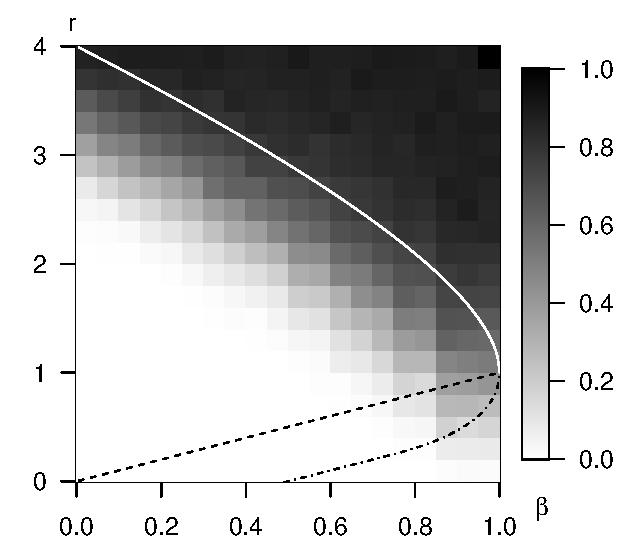
\includegraphics[width=0.4\textwidth]{./figures/simulated_phase_diagram_p100.eps}
      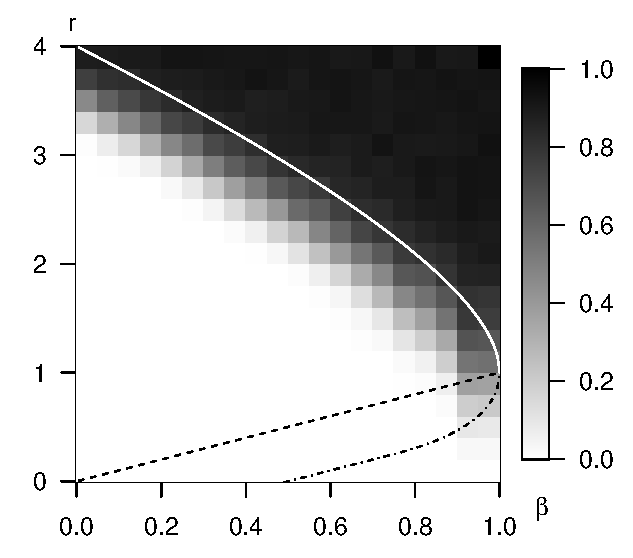
\includegraphics[width=0.4\textwidth]{./figures/simulated_phase_diagram_p10000.eps}
      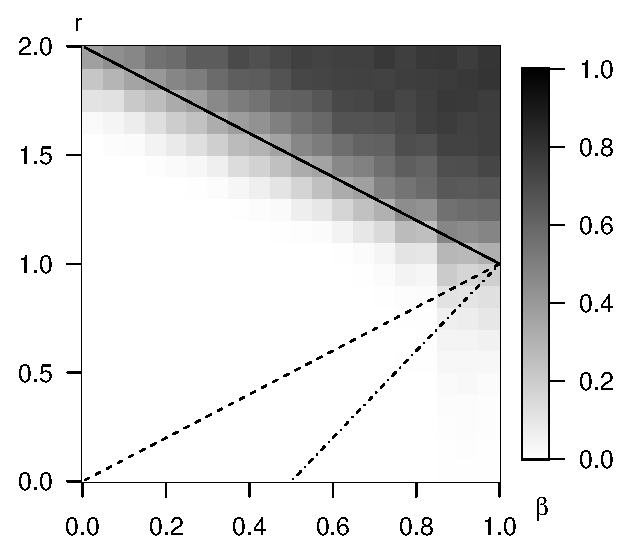
\includegraphics[width=0.4\textwidth]{./figures/simulated_phase_diagram_Laplace_p100_4.eps}
      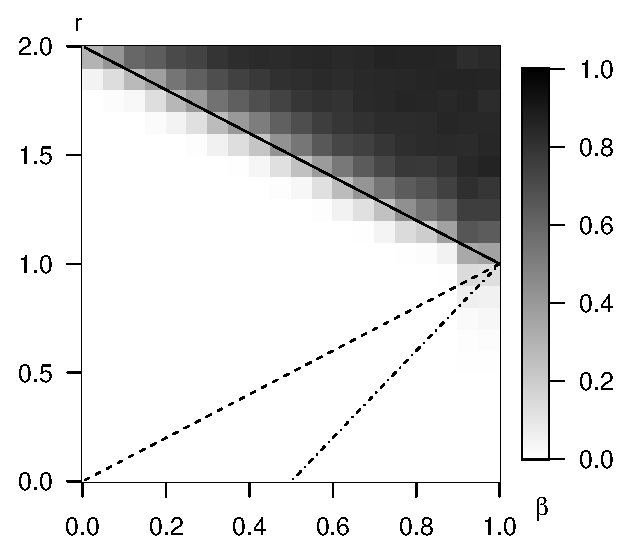
\includegraphics[width=0.4\textwidth]{./figures/simulated_phase_diagram_Laplace_p10000_4.eps}
      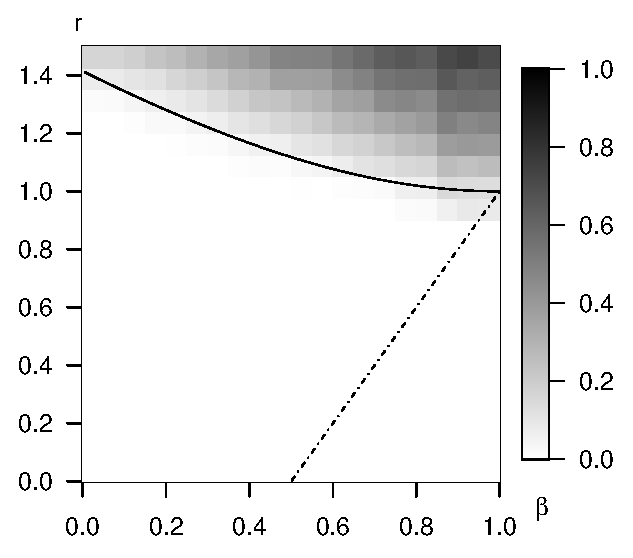
\includegraphics[width=0.4\textwidth]{./figures/simulated_phase_diagram_NLC_p100.eps}
      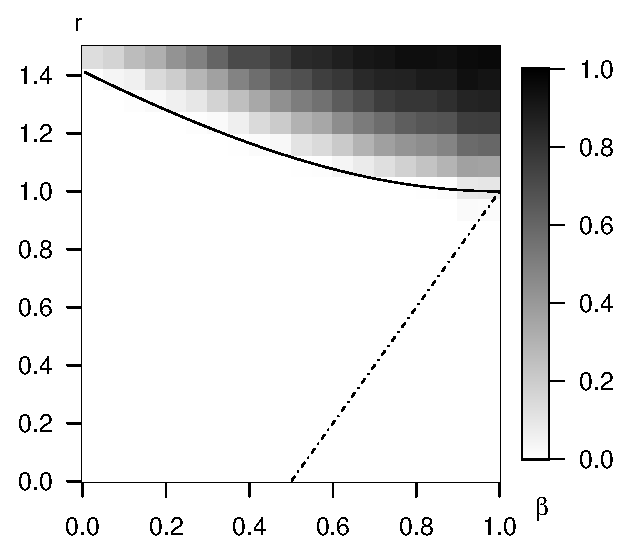
\includegraphics[width=0.4\textwidth]{./figures/simulated_phase_diagram_NLC_p10000.eps}
      \caption{The empirical probability of exact support recovery from numerical experiments, as a function of sparsity level $\beta$ and signal sizes $r$, 
      from Gaussian error models (upper panels), Laplace error models (middle panels), and generalized Gaussian with $\nu=1/2$ (lower panels); darker color indicates higher probability of exact support recovery. 
      The experiments were repeated 1000 times for each sparsity-signal size combination, and for dimensions $p=100$ (left panels) and $p=10000$ (right panels). 
      The numerical results agree with the boundaries described in Theorem \ref{thm:sufficient}. The convergence is noticeably slower for under the heavier 
      generalized Gaussian ($\nu=1/2$) errors.  For reference, the dashed and dash-dotted lines represent the weak classification and detection boundaries
       (see Chapter \ref{chap:phase-transitions}).
      \label{fig:phase-simulated}}
\end{figure}





%\section{Bayes minimax optimality and (sub)optimality of thresholding procedures}


%\section{Strong classification boundaries in other light-tailed error models}
%\label{suppsec:other-boundaries}
%The strong classification boundaries extend beyond the AGG models.
As our analysis in Section \ref{sec:boundary} suggests, all additive error models where the errors have URS maxima demonstrate this phase transition phenomenon under appropriate parametrization of the sparsity and signal sizes.
We derive explicit boundaries for two additional classes of models under the general form of the additive noise models \eqref{eq:model-additive}, with heavier and lighter tails than the AGG models, respectively. 

We would like to point out that the sparsity and signal sizes can be re-parametrized for the boundaries to have different shapes.
For example in the case of Gaussian errors, if we re-parametrize sparsity $s$ with 
$\widetilde{\beta} = 2 - \left(1 + \sqrt{1-\beta}\right)^2$ where $\widetilde{\beta}\in(0,1)$, then the signal sparsity would have a slightly more complicated form:
$$
\left|S_p\right| = \left\lfloor p^{1-\beta} \right\rfloor = \left\lfloor p^{\left(\sqrt{2 - \widetilde{\beta}} - 1\right)^2}\right\rfloor,
$$
while the strong classification boundary would take on the simpler form:
\begin{equation}\label{eq:altenative-parametrization}
g(\beta) = \widetilde{g}(\widetilde{\beta}) = 2 - \widetilde{\beta}.
\end{equation}
In the next two classes of models we will adopt parametrizations such that the boundaries are of the form $\widetilde{g}$ in \eqref{eq:altenative-parametrization}.

\subsection{Additive error models with heavier-than-AGG tails}

Distributions such as the log-normal have heavier tails than the AGG model, yet the tails are nevertheless rapidly-varying. 
Therefore, Proposition \ref{prop:rapid-varying-tails} applies, and we expect to see phase-transition-type results when the additive errors have these heavier-than-AGG tails.

\begin{example}[Heavier than AGG] \label{exmp:heavier-than-AGG}
Let $\gamma>1$, $c>0$, and suppose that
\begin{equation} \label{eq:heavier-than-AGG}
    \log{\overline{F}(x)} = - \left(\log x\right)^\gamma \left(c+M(x)\right),
\end{equation}
where $\lim_{x\to\infty} M(x)\log^\gamma{x}= 0$. Then, Relation \eqref{eq:rapid-varying-tails} holds under 
model \eqref{eq:heavier-than-AGG}. Further, if the entries in the array are independent, the 
maxima are relatively stable.

The behavior of the quantiles $u_p$ in this model is as follows. As $p\to\infty,$
\begin{equation*}
    u_p \sim \exp{\left\{\left(c^{-1}\log{p}\right)^{1/\gamma}\right\}}
    \iff c\left(\log{u_p}\right)^{\gamma} + o(1) = \log(p) = - \log \overline{F}(u_p).
\end{equation*}
since $u_p$ diverges, and $M(u_p)$ is $o((\log^\gamma u_p)^{-1})$.
\end{example}


Following Example \ref{exmp:heavier-than-AGG}, assume that the errors in Model \eqref{eq:model-additive} have rapidly varying right tails
\begin{equation} \label{eq:heavier-than-AGG-boundary-1}
    \log{\overline{F}(x)} = - \left(\log x\right)^\gamma \left(c+M(x)\right),
\end{equation}
as $x\to \infty$, and left tails
\begin{equation} \label{eq:heavier-than-AGG-boundary-2}
    \log{{F}(x)} = - \left(\log{(-x)}\right)^\gamma \left(c+M(-x)\right),
\end{equation}
as $x\to -\infty$.

\begin{theorem} \label{thm:heavier-than-AGG}
Suppose the marginals $F$ follows \eqref{eq:heavier-than-AGG-boundary-1} and \eqref{eq:heavier-than-AGG-boundary-2}.
Let
$$
k(\beta) = \log{p} - \left((\log{p})^{1/\gamma} + \log{(1-\beta)}\right)^\gamma,
$$
and let the signal $\mu$ have 
$$|S_p| = \left\lfloor pe^{-k(\beta)} \right\rfloor$$
non-zero entries. Assume the magnitudes of non-zero signal entries are in the range between
$$\underline{\Delta} = \exp{\left\{(\log{p})^{1/\gamma}\right\}}\underline{r}
\quad\text{and}\quad
\overline{\Delta} = \exp{\left\{(\log{p})^{1/\gamma}\right\}}\overline{r}.$$
If $\underline{r} > \widetilde{g}(\beta) = 2 - \beta$, then Bonferroni's procedure $\widehat{S}_p$ (defined in \eqref{eq:Bonferroni-procedure}) with appropriately calibrated FWER $\alpha\to 0$ achieves asymptotic perfect support recovery, under arbitrary dependence of the errors.

On the other hand, when the errors are uniformly relatively stable, if $\overline{r} < \widetilde{g}(\beta) = 2 - \beta$, then no thresholding procedure can achieve asymptotic perfect support recovery with positive probability.
\end{theorem}


\subsection{Additive error models with lighter-than-AGG tails}


Similar to how Proposition \ref{prop:rapid-varying-tails} applies to models with heavier-than-AGG tails, it also to error models with lighter tails than the AGG class.

\begin{example}[Lighter than AGG] \label{exmp:lighter-than-AGG}
With $\nu>0$, and $L(x)$ a slowly varying function, the class of distributions
\begin{equation} \label{eq:lighter-than-AGG}
    \log{\overline{F}(x)} = - \exp{\left\{x^\nu L(x)\right\}},
\end{equation}
is rapidly varying.
The quantiles can be derived explicitly in a subclass of \eqref{eq:lighter-than-AGG} where $L(x)\to 1$, or equivalently, when $\log{|\log{\overline{F}(x)}|}\sim x^\nu$,
\begin{equation*}
    u_p \sim \left(\log \log{p}\right)^{1/\nu}
    \iff \exp{\left\{u_p^\nu\left(1+o(1)\right)\right\}} = \log(p) = - \log \overline{F}(u_p).
\end{equation*}
\end{example}
%The proofs of the rapid variation of the distributions in Examples \ref{exmp:heavier-than-AGG} and \ref{exmp:lighter-than-AGG} are entirely analogous to that of Example \ref{exmp:AGG}, and omitted.


Following Example \ref{exmp:lighter-than-AGG}, assume that errors in Model \eqref{eq:model-additive} has rapidly varying right tails
\begin{equation} \label{eq:lighter-than-AGG-boundary-1}
        \log{\overline{F}(x)} = - \exp{\left\{x^\nu L(x)\right\}},
\end{equation}
where $L(x)$ is a slowly varying function, as $x\to\infty$, and left tails
\begin{equation} \label{eq:lighter-than-AGG-boundary-2}
        \log{\overline{F}(x)} = - \exp{\left\{-x^\nu L(-x)\right\}},
\end{equation}
as $x\to -\infty$.

The phase transition results in multiple testing problems under such tail assumptions is characterizes as follows.

\begin{theorem} \label{thm:lighter-than-AGG}
Suppose marginals $F$ follow \eqref{eq:lighter-than-AGG-boundary-1} and \eqref{eq:lighter-than-AGG-boundary-2}.
Let
$$
k(\beta) = \log{p} - \left(\log(p)\right)^{(1-\beta)^\nu},
$$
and let the signal $\mu$ have 
$$|S_p| = \left\lfloor pe^{-k(\beta)} \right\rfloor$$
non-zero entries. Assume the magnitudes of non-zero signal entries are in the range between
$$\underline{\Delta} = \log{\log{p}}^{1/\nu}\underline{r}
\quad\text{and}\quad
\overline{\Delta} = \log{\log{p}}^{1/\nu}\overline{r}.$$
If $\underline{r} > \widetilde{g}(\beta) = 2 - \beta$, then Bonferroni's procedure $\widehat{S}_p$ (defined in \eqref{eq:Bonferroni-procedure}) with appropriately calibrated FWER $\alpha\to 0$ achieves asymptotic perfect support recovery, under arbitrary dependence of the errors.

On the other hand, when the errors are uniformly relatively stable, if $\overline{r} < \widetilde{g}(\beta) = 2 - \beta$, then no thresholding procedure can achieve asymptotic perfect support recovery with positive probability.
\end{theorem}





%\section{Thresholding procedures under heavy-tailed errors}
%\label{suppsec:heavy-tailed}
%We analyze the performance of thresholding estimators under heavy-tailed models in this section, and illustrate its lack of phase transition.
Suppose we have iid errors with Pareto tails in Model \eqref{eq:model-additive}, that is, $\epsilon(i)$'s have common marginal distribution $F$ where
\begin{equation} \label{eq:pareto-tails}
    \overline{F}(x) \sim x^{-\alpha} \quad \text{and} \quad F(-x) \sim x^{-\alpha},    
\end{equation}
as $x\to\infty$. 
It is well-known (see, e.g., Theorem 1.6.2 of \citep{leadbetter2012extremes}) that the maxima of iid Pareto random variables have Frechet-type limits.
Specifically, we have
\begin{equation} \label{eq:Frechet-limit-1}
    \frac{\max_{i\in\{1,\ldots,p\}}\epsilon(i)}{u_p} \implies Y,
\end{equation}
in distribution, where $u_p = F^{\leftarrow}(1-1/p)\sim p^{1/\alpha}$, and $Y$ is a standard $\alpha$-Frechet random variable, i.e.,
\begin{equation*}
    \P[Y\le t] = \exp{\{-t^{-\alpha}\}}, \quad t>0.
\end{equation*}
By symmetry in our assumptions, the same argument applies to the minima as well.

\begin{theorem} \label{thm:heavy-tails}
Let errors in Model \eqref{eq:model-additive} be as described in Relation \eqref{eq:pareto-tails}.
Let the signal have $s = |S| = fp$ non-zero entries, with magnitude $\Delta = rp^{1/\alpha}$, where both $f\in(0,1)$ and $r\in(0,+\infty)$ may depend on $p$, so that no generality is lost.

Under these assumptions, the necessary condition for thresholding procedures $\widehat{S}$ to achieve exact support recovery ($\P[\widehat{S}=S]\to1$) is 
\begin{equation} \label{eq:heavy-tails-exact-recovery}
    \liminf_{p\to\infty} r = \infty.
\end{equation}
Condition \eqref{eq:heavy-tails-exact-recovery} is also sufficient for the oracle thresholding procedure to succeed in the exact support recovery problem.

On the other hand, the necessary and sufficient condition for all thresholding procedures to fail exact support recovery ($\P[\widehat{S}=S]\to0$) is 
$$
\limsup_{p\to\infty} r = 0.
$$
\end{theorem}

In other words, Theorem \ref{thm:heavy-tails} states that there does not exist a non-trivial phase transition for thresholding procedures when errors have (two-sided) $\alpha$-Pareto tails.

\begin{proof}[Proof of Theorem \ref{thm:heavy-tails}]
Recall the oracle thresholding procedure $\widehat{S}^* = \left\{i:x(i) \ge x_{[s]}\right\}$, and the set of all thresholding procedures, denoted 
${\cal S}$ (see Definition \ref{eq:thresholding-procedure}).
The probability of exact support recovery by any thresholding procedure $\widehat{S}\in{\cal S}$ is bounded above by that of $\widehat{S}^*$, that is,
\begin{align}
    \max_{\widehat{S}\in{\cal S}}\P[\widehat{S}=S] 
        &= \P[\widehat{S}^*=S] 
        = \P\Big[\max_{i\in S^c}x(i) \le \min_{i\in S}x(i)\Big] \nonumber \\
        &= \P\Big[\frac{\max_{i\in S^c}x(i)}{u_p} \le \frac{\min_{i\in S}x(i)}{u_p}\Big] \nonumber \\
        &= \P\Big[\frac{M_{S^c}}{u_p} \le \frac{m_S}{u_p} + r_p\Big], \label{eq:heavy-tailed-case-proof-0}
        % &= \P\Big[\underbrace{(1-f)^{1/\alpha}Y^{(1)}}_{=:F_1} + \underbrace{f^{1/\alpha}Y^{(2)}}_{=:F_2} \le r\Big], 
\end{align}
where $M_{S^c} = \max_{i\in S^c}\epsilon(i)$ and $m_S = \min_{i\in S}\epsilon(i)$.
For any $\alpha > 0$, the following elementary relations hold,
\begin{equation*}
    0 < L \le (1-f)^{1/\alpha} + f^{1/\alpha} \le U < \infty, \quad \text{for all} \; f\in(0,1),
\end{equation*}
where $L = \min\left\{1, 2(1/2)^{1/\alpha}\right\}$ and $U = \max\left\{1, 2(1/2)^{1/\alpha}\right\}$.
Therefore we have,
\begin{equation} \label{eq:heavy-tailed-case-proof-1}
    U\max\left\{\frac{M_{S^c}}{u_p}, -\frac{m_S}{u_p}\right\} < r_p
    \implies
    (1-f)^{1/\alpha}\frac{M_{S^c}}{u_p} - f^{1/\alpha}\frac{m_S}{u_p} < r_p,
\end{equation}
and 
\begin{equation} \label{eq:heavy-tailed-case-proof-2}
    L\min\left\{\frac{M_{S^c}}{u_p}, -\frac{m_S}{u_p}\right\} < r_p
    \impliedby
    (1-f)^{1/\alpha}\frac{M_{S^c}}{u_p} - f^{1/\alpha}\frac{m_S}{u_p} < r_p.
\end{equation}
Putting together \eqref{eq:heavy-tailed-case-proof-0}, \eqref{eq:heavy-tailed-case-proof-1}, and \eqref{eq:heavy-tailed-case-proof-2}, we have
\begin{equation} \label{eq:heavy-tailed-case-proof-3}
    \P\Big[\max\left\{\frac{M_{S^c}}{u_p}, -\frac{m_S}{u_p}\right\} < r_p/U\Big]
    \le \P[\widehat{S}^*=S]
    \le \P\Big[\min\left\{\frac{M_{S^c}}{u_p}, -\frac{m_S}{u_p}\right\} < r_p/L\Big].
\end{equation}
We know from the weak convergence result \eqref{eq:Frechet-limit-1} that for any $\epsilon>0$ there is a constant $N$ such that for all $p>N$ we have 
\begin{equation} \label{eq:heavy-tailed-case-proof-3.5}
    \P\Big[\max\left\{\frac{M_{S^c}}{u_p}, -\frac{m_S}{u_p}\right\} < r_p/U\Big]
    \ge \P\Big[\max\left\{Y^{(1)}, Y^{(2)}\right\} < {r_p}/{U}\Big] - \epsilon,
\end{equation}
where $Y^{(1)}$ and $Y^{(2)}$ are independent $\alpha$-Frechet random variables with scale coefficients $(1-f)^{1/\alpha}$ and $f^{1/\alpha}$ respectively.
That is,
\begin{equation*}
    \P[Y^{(1)}\le t] = \exp{\{-(1-f)/t^\alpha\}}, 
    \quad \text{and} \quad
    \P[Y^{(2)}\le t] = \exp{\{-f/t^\alpha\}}.
\end{equation*}
Since the distributional limit in \eqref{eq:heavy-tailed-case-proof-3.5} has a density (with respect to the Lebesgue measure), we know that density is bounded above by a finite constant, say, $K$.
For the same choice of $\epsilon$ as before, we can find a further constant $N'$ such that for all $p>\max\{N, N'\}$ we have 
$$
    \liminf r_p < \epsilon/K + r_p,
$$
so that the right hand side of \eqref{eq:heavy-tailed-case-proof-3.5} is bounded by
\begin{equation} \label{eq:heavy-tailed-case-proof-3.6}
    \P\Big[\max\left\{Y^{(1)}, Y^{(2)}\right\} < {r_p}/{U}\Big] - \epsilon
    \ge \P\Big[\max\left\{Y^{(1)}, Y^{(2)}\right\} < \frac{\liminf r_p}{U}\Big] - 2\epsilon.
\end{equation}
By the arbitrariness in the choice of $\epsilon$, we conclude from \eqref{eq:heavy-tailed-case-proof-3.5} and \eqref{eq:heavy-tailed-case-proof-3.6} that
\begin{equation} \label{eq:heavy-tailed-case-proof-4}
    \liminf \P\Big[\max\left\{\frac{M_{S^c}}{u_p}, -\frac{m_S}{u_p}\right\} < r_p/U\Big]
    \ge \P\Big[\max\left\{Y^{(1)}, Y^{(2)}\right\} < \frac{\liminf r_p}{U}\Big].
\end{equation}
Combining Relations \eqref{eq:heavy-tailed-case-proof-3} and \eqref{eq:heavy-tailed-case-proof-4}, we know that if $\liminf r_p = \infty$, we must have 
$$
    \liminf\P\left[\widehat{S}^*=S\right]
    \ge \P\Big[\max\left\{Y^{(1)}, Y^{(2)}\right\} < \frac{\liminf r_p}{U}\Big] = 1.
$$
Conversely, if $\liminf\P\left[\widehat{S}^*=S\right]<1$, we must have $\liminf r_p < \infty$.

Similarly, we can obtain the upper bound of exact support recovery probability for the optimal thresholding procedure,
\begin{equation} \label{eq:heavy-tailed-case-proof-5}
    \limsup \P\Big[\min\left\{\frac{M_{S^c}}{u_p}, -\frac{m_S}{u_p}\right\} < r_p/L\Big]
    \le \P\Big[\min\left\{Y^{(1)}, Y^{(2)}\right\} < \frac{\limsup r_p}{L}\Big].
\end{equation}
The conclusions of the second part of Theorem \ref{thm:heavy-tails} follow from \eqref{eq:heavy-tailed-case-proof-3} and \eqref{eq:heavy-tailed-case-proof-5}.
\end{proof}

The probability of exact recovery can be approximated if the parameters $r$ and $f$ converge.
The next result follows from a small modification of the arguments in the proof of Theorem \ref{thm:heavy-tails}.

\begin{corollary}
Under the assumptions in Theorem \ref{thm:heavy-tails}, if 
$\lim r = r^*$, and $\lim f = f^*$, for some constant $r^*\ge0$ and $f^*\in[0,1]$, then 
$$
    \lim \P[\widehat{S}^*=S] 
    = \P\Big[(1-f^*)^{1/\alpha}Z_1 + (f^*)^{1/\alpha}Z_2 < {r^*}\Big].
$$
where $Z_1$ and $Z_2$ are independent standard $\alpha$-Frechet random variables, i.e., $\P[Z_i \le t] = \exp{\{-x^{-\alpha}\}}$, $x>0$.
\end{corollary}

\begin{remark}
Of course one might wonder if it would be meaningful to derive a ``phase transition'' under a different parametrization of the signal sizes, say 
\begin{equation} \label{eq:Pareto-parametrization-with-boundary}
    \Delta = p^{r/\alpha}.
\end{equation}
In this case, Theorem \ref{thm:heavy-tails} suggests that a ``phase transition'' takes place at $r=1$.
However, this non-multiplicative parametrization of the signal sizes would make power analysis (like in Example \ref{exmp:gap-when-signal-sparse}) dimension-dependent. 

To illustrate, in the case of Gaussian errors with variance 1, if we were interested in small signals of size $\sqrt{2r\log{p}}$, where $r<1$ is below the boundary \eqref{eq:strong-classification-boundary}, then we only need $n > 2/r$ samples to guarantee discovery of their support.
In the Pareto case with parametrization \eqref{eq:Pareto-parametrization-with-boundary}, however, if we were interested in small signals of size $p^{r/\alpha}$, where $r<1$, then the ``boundary'' says that we will need $n > p^{2(1-r)/\alpha}$ samples, which is exponential in the dimension $p$ and quickly diverges.
Recall that the ``boundary'' is really an asymptotic result in $p$. 
Such an approximation in finite dimensions becomes invalid.
\end{remark}









\chapter{\comment{Characterization of} Uniform Relative Stability for Gaussian Arrays}
\label{chap:URS}

In this chapter, we establish a complete characterization of URS for Gaussian arrays in terms of a simple condition on the covariance structures.
The condition is as follows.

% The proof of the main result is deferred until Section \ref{sec:proofs}.

% We define the class of dependence structures, referred to as uniformly decreasing dependence (UDD), for Gaussian arrays via their covariance matrices.

\begin{definition}[Uniformly decreasing dependence (UDD)] \label{def:UDD}
Consider a triangular array of jointly Gaussian distributed errors 
${\cal E} = \left\{\left(\epsilon_p(i)\right)_{i=1}^p, p = 1,2,\ldots\right\}$ 
with unit variances,
$$
\epsilon_p \sim \text{N}(0, \Sigma_p), \quad p=1,2,\ldots.
$$
The array ${\cal E}$ is said to be uniform decreasingly dependent (UDD) if 
for every $\delta>0$ there exists a finite $N(\delta)<\infty$, such that for every $i\in\{1,\ldots,p\}$, and $p\in\N$, we have
\begin{equation} \label{eq:UDD-definition}
    \Big|\left\{k\in\{1,\ldots,p\}:\Sigma_p(i,k)>\delta\right\}\Big| \le N(\delta)\quad \text{for all  } \delta>0.
\end{equation}
\end{definition}
That is, for every coordinate $i$, the number of elements which are more than $\delta$-correlated with $\epsilon_p(i)$ does not exceed $N(\delta)$. 

Note that the bound in \eqref{eq:UDD-definition} holds uniformly in $i$ and $p$, and only depends on $\delta$.
Also observe that on the left-hand side of \eqref{eq:UDD-definition}, we merely count in each row of $\Sigma_p$ the number of exceedances of covariances (not their absolute values!) over level $\delta$.

\begin{remark} \label{rmk:choice-of-N(delta)}
Without loss of generality, we may require that $N(\delta)$ be a monotone non-increasing function of $\delta$, for we can take
$$
N(\delta) = \sup_{p,i} \Big|\{k:\Sigma_p(i,k)>\delta\}\Big|,
$$
which is non-increasing in $\delta$.
Definition \ref{def:UDD} therefore states that the array is UDD when $N(\delta)<\infty$ for all $\delta>0$.
\end{remark}


Observe that the UDD condition does not depend on the order of the coordinates in the error 
vector $\epsilon_p = (\epsilon_p(i))_{i=1}^p$.  Often times, however, the errors are thought of 
coming from a stochastic process indexed by time or space.  To illustrate the generality of the 
UDD condition, we formulate next a simple sufficient condition (UDD$^\prime$) that is easier to 
check in a time-series context.

\begin{definition}[UDD\,$^\prime$]\label{d:UDD-prime}
For $\epsilon_p \sim \mathrm{N}(0,\Sigma_p)$ with unit variances, an array ${\cal E} = \left(\epsilon_p(i)\right)_{i=1}^p$ is said to satisfy the UDD\,$^\prime$ condition if there 
exist:
\begin{enumerate}
    \item[(i)] permutations $l = l_p$ of $\{1,\ldots,p\}$, for all $p\in\N$, and
    \item[(ii)] a non-negative sequence $(r_n)_{n=1}^\infty$ converging to zero $r_n\to 0$, as $n\to\infty$,
\end{enumerate}
such that 
\begin{equation} \label{eq:weak-correlation}
    \sup_{p\in\N} |\Sigma_p\left(i',j'\right)| \le r_{|i-j|}.
\end{equation}
where $i' = l(i)$, $j' = l(j)$, for all $i,j\in\{1,\ldots,p\}$.
\end{definition}

\begin{remark}
Without loss of generality, we may also require that $r_n$ be non-increasing in $n$, for we can replace $r_n$ with the non-increasing sequence $r'_n = \sup_{m\ge n} r_m$.
\end{remark}

\begin{proposition} \label{prop:UDD-equivalent}
UDD\,$^\prime$ implies UDD.
\end{proposition} 

\begin{proof}%[Proof of Proposition \ref{prop:UDD-equivalent}]
%The functions $N(\delta)$ and $r(n)=r_n$ are inverses of each other.
% {\bf $\text{UDD} \implies \text{UDD'}$:}
% If $N(0)<\infty$, then we can take 
% $$
% r_n = \underbrace{1, \ldots, 1}_{\lfloor N(0)/2\rfloor + 1}, 0, 0, \ldots.
% $$
% and recursively construct the permutations as follows.
% Start with any element

% We proof the contrapositive. 
% Suppose for all permutations and any sequence $r_n\to0$, there exists $i,j$ such that $\Sigma(i',j')>r_{|i'-j'|}$,
% then for any $\delta>0$ and any finite $M<\infty$, we can take $r_n$ to be a sequence of $M$ 1's followed by a $\delta$, i.e., 
% $$
% r_n = \underbrace{1, \ldots, 1}_{M+1}, \delta, \ldots.
% $$
% \fbox{Not true:}
% However, since there exists $i',j'$ such that $\Sigma(i',j')>r_{|i'-j'|}$, the set 
% $$
% S = l^{-1}\left(\left\{j',i'-N,\ldots,i'-1,i',i'+1,\ldots,i'+N\right\}\right)
% $$ 

% {\bf $\text{UDD'} \implies \text{UDD}$:} 
Since $r_n\to 0$, for any $\delta > 0$, there exists an integer 
$M = M(\delta)<\infty$ such that $r_n\le\delta$, for all $n\ge M$. 
Thus, by \eqref{eq:weak-correlation}, for every fixed 
$j' \in\{1,\ldots,p\}$, we can have $|\cov(\epsilon_p(k'),\epsilon_p(j'))| > \delta$,
only if $k'$ belongs to the set:
$$ 
 \left\{ k' \in \{1,\dots,p\} \, :\, j-M \le  k := l_p^{-1}(k') \le j+M \right\},
$$
where $j:= l_p^{-1}(j')$. That is, there are at most $2M+1<\infty$ indices  $k'\in\{1,\dots,p\}$, whose covariances with $\epsilon(j')$ may exceed $\delta$. 
Since this holds uniformly in $j'\in\{1,\ldots,p\}$, Condition UDD follows with 
$N(\delta) = 2M+1$.
\end{proof}



% \begin{definition}[Uniformly decreasing dependence (UDD)] \label{def:weak-dependence}
% Consider a triangular array of jointly Gaussian distributed errors $\left(\epsilon_p(j)\right)_{j=1}^p$ with unit variances, $\epsilon_p \sim \mathcal N(0,\Sigma_p)$. The array ${\cal E}$ is said to be uniform decreasingly dependent (UDD) with rate $(r_n)_{n=1}^\infty$ if 
% \begin{equation} \label{eq:weak-correlation}
%     \sup_p |\Sigma_p(i,j)| \le r_{|i-j|}
% \end{equation}
% such that $r_n\to 0$, as $n\to\infty$.
% \end{definition}
% 
% \begin{remark} \label{rmk:UDD-equivalent}
% In situations where there is no natural ordering of the components, it is sufficient that a permutation of the vector $\epsilon$ in its coordinates satisfy the requirements above. 
% In fact, the UDD condition can be equivalently stated as follows: for any $\delta>0$, and any coordinate $j\in\{1,\ldots,p\}$, there are at most $N(\delta)<\infty$ coordinates whose covariances with $\epsilon(j)$ exceed $\delta$; here $N(\delta)$ is a deterministic function independent of $p$.
% $N(\delta) \to 1$ as $\delta \to 0$.
% \end{remark}

We now state the main result of this section: a Gaussian sequence is URS if and only if it is UDD.
The URS condition essentially requires that the dependencies decay in a uniform fashion, the rate at which dependence decay does \emph{not} matter.

\begin{theorem} \label{thm:Gaussian-weak-dependence}
Let ${\cal E}$ be a Gaussian triangular array with standard normal marginals.  
The array ${\cal E}$ has uniformly relatively stable (URS) maxima if and only if it is uniformly decreasing dependent (UDD).
\end{theorem}

% The proof of Theorem \ref{thm:Gaussian-weak-dependence} is given in Section \ref{sec:proofs}. 

Specifically, for stationary Gaussian arrays, we have the following corollary.

\begin{corollary} \label{cor:stationary-Gaussian-errors}
Let ${\cal E} = \{\epsilon_p(i) = Z(i)\}$ for a stationary Gaussian time series ${\cal Z} = \{Z(i)\}$.
Then $\cal E$ is {URS} if and only if the autocovariance function $\cov(Z(k), Z(0))\to 0$, as $k\to\infty$.
\end{corollary}

Corollary \ref{cor:stationary-Gaussian-errors} follows by Theorem \ref{thm:Gaussian-weak-dependence} and the observation that UDD is equivalent to vanishing autocovariance of $\cal Z$.
A slightly weaker form of the ``if'' part was established in Theorem 3 of \cite{berman1964limit}.

Returning again to the study of support recovery problems, Theorem \ref{thm:Gaussian-weak-dependence} and the necessary condition for exact support recovery in Theorem \ref{thm:necessary} yields the following result.

\begin{corollary} \label{cor:weakly-dependent-errors}
For UDD Gaussian errors, the result in Theorem \ref{thm:necessary} holds.
\end{corollary}

As a counterpart to Remark \ref{rmk:dependence-assumptions}, we demonstrate the tightness of the dependence conditions in Theorem \ref{thm:necessary}.
Specifically, we demonstrate that if the URS dependence condition is violated, then it may be possible to recover the support of weaker signals below the boundary.

\begin{example} \label{exmp:counter-example}
Suppose ${\cal E} = \left(\epsilon_p(i)\right)_{i=1}^p$ is Gaussian, and is comprised of $\lfloor p^{1-\beta}\rfloor$ blocks, each of size at least $\lfloor p^\beta \rfloor$; 
let the elements of each block have correlation 1, and let elements from different blocks be independent. 
If $\underline{r} \ge 4(1-\beta)$, then the procedure $\widehat{S} = \big\{i:x(i)>\sqrt{2(1-\beta)\log{p}}\big\}$ yields $\mathbb P[\widehat{S} = S] \to 1$. 
This requirement on signal size is strictly weaker than that of the strong classification boundary, since $4(1-\beta) < (1 + \sqrt{1-\beta})^2$ on $\beta\in(0,1)$.
\end{example} 

The above example shows that if the correlations of the Gaussian errors do not decay in a uniform fashion (UDD fails), then we can do substantially better in terms of support recovery.
The claims in the example are verified in Section \ref{suppsec:proofs}, while numerical simulations of this example can be found in Section \ref{suppsec:numerical}.

\medskip

We conclude with a brief discussion on the relationships between UDD and other dependence conditions in the context of extreme value theory, before proceeding to the proof of Theorem \ref{thm:Gaussian-weak-dependence}.

Suppose that the array of errors  ${\cal E}$ comes from a stationary Gaussian time series $\epsilon(i),\ i\in \mathbb{N}$, with auto-covariance $r_p=\cov(\epsilon(i+p),\epsilon(i))$. 
One is interested in the asymptotic behavior of the maxima $M_p:=\max_{i=1,\dots,p} \epsilon(i)$.

In this setting, the Berman's condition, introduced in \cite{berman1964limit}, requires that
\begin{equation} \label{eq:Berman}
    r_p \log p \to 0,\ \ \mbox{ as }p\to\infty.
\end{equation}
This condition entails that 
\begin{equation}
    \label{eq:Gauss-max-in-distribution}
  a_p (M_p - b_p) \stackrel{d}{\longrightarrow } Z,\  \ \mbox{ as }p\to\infty,
\end{equation}
with the Gumbel limit distribution $\mathbb P [Z\le x] = \exp\{-e^{-x}\},\ x\in \mathbb R$, 
where 
$$
a_p = \sqrt{2\log p},\quad b_p  = \sqrt{2\log p} - \frac{1}{2}\left(\sqrt{2\log p}\right)^{-1}\left(\log \log (p) + \log(4\pi)\right),
$$ 
are {\em the same} centering and normalization sequences
as in the case of iid $\epsilon(i)$'s.  
Berman's condition is one of the weakest dependence conditions  in the literature for which this result holds. See, e.g., Theorem 4.4.8 in \cite{embrechts2013modelling}, where \eqref{eq:Berman} is described as ``very weak''.

For dependence conditions weaker than \eqref{eq:Berman}, the sequences of normalizing and centering constants in \eqref{eq:Gauss-max-in-distribution} are {\em different} from the iid case, and the corresponding limit is no longer Gumbel; see, for example, Theorems 6.5.1 and  6.6.4 in \cite{leadbetter2012extremes}, and \cite{mccormick1976weak}. 
% In particular, \cite{mccormick1976weak} derived the normalizing constants when both $r_p\to 0$ monotonically and  $r_p \log p \to \infty$ monotonically, as $p\to\infty$. 
% In this case, convergence in distribution still takes place, with the maxima concentrating along a sequence asymptotic to \eqref{eq:quantiles}.

On the other hand, in our high dimensional support estimation context, the notion of relative stability is sufficient and more natural than the finer notions of distributional convergence.
If one is merely interested in the asymptotic relative stability of the Gaussian maxima, then Berman's condition can be relaxed significantly (see also, Theorem 4.1 of \cite{berman1964limit}). 
Observe that by Proposition \ref{prop:UDD-equivalent},  the Berman condition \eqref{eq:Berman} implies UDD and hence relative stability (Theorem \ref{thm:Gaussian-weak-dependence}), i.e., 
\begin{equation} \label{eq:Gaussian-URS}
  \frac{1}{b_p} M_p \stackrel{\mathbb P}{\to} 1,\quad\mbox{as}\quad p\to\infty.
\end{equation}
This {\em concentration of maxima} property can be readily deduced from \eqref{eq:Gauss-max-in-distribution}, since $a_p b_p \sim 2\log(p) \to \infty$ as $p\to\infty$.
Theorem \ref{thm:Gaussian-weak-dependence} shows that \eqref{eq:Gaussian-URS} holds if the much weaker uniform dependence condition UDD holds. 
Note that our condition is coordinate free --- neither monotonicity of the sequence $r_p$ nor stationarity of the underlying array is required. 

% The method of proof is also very different from the results on distributional convergence in the references mentioned above. 

\medskip

The rest of this chapter is devoted to the proof of the main result, i.e., Theorem \ref{thm:Gaussian-weak-dependence}. 
We first introduce a key lemma regarding the structure of correlation matrix of high-dimensional random variables.
The proof uses a surprising, yet elegant application of Ramsey's Theorem from the study of combinatorics.
%; this application, and its consequences in high-dimensional probability, are presented in Section \ref{subsec:Ramsey}.
The `only if' part of Theorem \ref{thm:Gaussian-weak-dependence} follows from this lemma, in Section \ref{sec:URS=>UDD}. 

The proof of the `if' part is detailed in Section \ref{sec:UDD=>URS}.
The arguments there was recently extended to establish bounds on the rate of concentration of maxima in \cite{kartsioukas2019rate}; see also, \cite{tanguy2015some} and references therein for related work on this topic.

\section{Ramsey's Coloring theorem and structure of correlation matrices} 
\label{sec:Ramsey}


% We start by providing a general result on the structure of arbitrary correlation matrices in this section, which helps us establish the `only if' part of Theorem \ref{thm:Gaussian-weak-dependence}. 
% Its proof uses the Ramsey Theorem from graph theory, which we briefly review next.

Given any integer $k\ge 1$, there is always an integer $R(k,k)$ called the {\em Ramsey number}:
\begin{equation}\label{eq:Ramsey-number}
k\le R(k,k)\le \binom{2k-2}{k-1}
\end{equation}
such that the following property holds:
every undirected graph with at least $R(k,k)$ vertices will contain {\em either} a clique of size $k$, or an {\em independent set} of $k$ nodes. 
Recall that a clique is a complete sub-graph where all pairs of nodes are connected, and an independent set is a set of nodes where no two nodes are connected.

This result is a consequence of the celebrated work of \citet{ramsey2009problem}, which 
gave birth to Ramsey Theory \citep[see e.g.,][]{conlon2015recent}.  
The Ramsey Theorem and the upper bound \eqref{eq:Ramsey-number} \citep[established first in][]{erdos1935combinatorial} are at the heart of the proof of the following result.  A recent improvement on the upper bound is given by \cite{sah:2020}.
%An excellent introduction to Ramsey theory is given in \url{http://math.mit.edu/~fox/MAT307-lecture05.pdf}. 

\begin{proposition} \label{prop:lower-bound-correlation-Ramsey}
  Fix $\gamma\in(0,1)$ and let $P = \left(\rho(i,j)\right)_{n\times n}$ be an arbitrary correlation
  matrix. If 
  \begin{equation}\label{eq:Ramsey-the-k-def}
   k:= \lfloor \log_2({n})/2 \rfloor  \ge \lceil 1/\gamma \rceil + 1,
  \end{equation}
  then there is a set of $k$ indices $K = \{l_1, \ldots, l_k\}\subseteq \{1,\ldots,n\}$ 
  such that 
  \begin{equation} \label{eq:lower-bound-correlation-Ramsey}
      \rho(i,j) \ge -\gamma, \mbox{ for all } i,j\in K.
  \end{equation}
\end{proposition}

\begin{proof}%[Proof of Proposition \ref{prop:lower-bound-correlation-Ramsey}]
By using \eqref{eq:Ramsey-number} and a refinement of the Stirling's formula, 
we will show at the end of the proof that for $k \le \log_2({n})/2$, we have 
\begin{equation}\label{eq:Ramsey-bounds}
 R(k,k) \le n,
\end{equation}
where $R(k,k)$ is the Ramsey number.  

Now, construct a graph with vertices $\{1,\dots,n\}$ such that there is an edge between nodes $i$ and $j$ if and only if $\rho(i,j) \ge -\gamma$. 
In view of \eqref{eq:Ramsey-bounds} and Ramsey's theorem (see e.g., Theorem 1 in \cite{fox2009lecture} or \cite{conlon2015recent} for a recent survey on Ramsey theory), there is a subset of $k$ nodes $K =\{l_1,\dots,l_k\}$, which is either a {\em complete graph} or an {\em independent set}.  Recall that in a
complete graph, every two nodes are connected with an edge; while in independent sets, no two nodes are connected.

If $K$ is a complete graph, then by our construction of the graph, Relation \eqref{eq:lower-bound-correlation-Ramsey} holds. 

Now, suppose that $K$ is a set of independent nodes.  This means, again by the construction of our graph, that
$$
\rho(i,j) < -\gamma,\quad\mbox{for all }i\not= j\in K.
$$
Let $Z_i,\ i \in K$ be zero-mean random variables such that 
$\rho(i,j) = \E [Z_iZ_j]$. Observe that
\begin{equation} \label{eq:Ramsey-proof-contradiction}
    \var\left( \sum_{i\in K} Z_i\right) 
    = \sum_{i\in K} \var(Z_i) + \sum_{\substack{i\not=j\\i,j \in K}} \cov(Z_i, Z_j) 
    <  k - k(k-1)\gamma,
\end{equation}
since $\var(Z_i)=1$ and $\rho(i,j)<-\gamma$ for $i\neq j$.
By our assumption, $k\ge \left(\lceil 1/\gamma \rceil + 1\right)$, or equivalently, $(k-1) \ge 1/\gamma$, the variance in \eqref{eq:Ramsey-proof-contradiction} is negative. 
This is a contradiction showing that there are no independent sets $K$ with cardinality $k$.

To complete the proof, it remains to show that Relation \eqref{eq:Ramsey-bounds} holds.
In view of the upper bound on the Ramsey numbers \eqref{eq:Ramsey-number}, it 
is enough to show that $k \le \log_2(\sqrt{n})$ implies
$$
\binom{2k-2}{k-1} \le n.
$$
This follows from a refinement of the Stirling formula, due to \citet{robbins1955remark}:
$$
 \sqrt{2\pi} m^{m+1/2} e^{-m} e^{\frac{1}{(12 m +1)}} \le  m! \le \sqrt{2\pi} m^{m+1/2} e^{-m} 
 e^{\frac{1}{12 m}}.
$$
Indeed, letting $\widetilde k:= k-1$, and applying the above upper and lower bounds 
to the  terms $(2\widetilde k)!$ and $\widetilde k!$, respectively, we obtain:
\begin{align*}
\binom{2k-2}{k-1} \equiv \frac{(2\widetilde k)!}{ (\widetilde k!)^2 }
\le \frac{2^{2\widetilde k}}{\sqrt{\pi \widetilde k}}\exp\left \{ \frac{1}{24 \widetilde k} -
\frac{2}{ 12 \widetilde k +1}\right\} < 2^{2 k}
\end{align*}
where the last two inequalities follow by simply dropping positive factors less than $1$.
Since $2k \le \log_2(n)$, the above bound implies Relation \eqref{eq:Ramsey-bounds} 
and the proof is complete.
\end{proof}

Using Proposition \ref{prop:lower-bound-correlation-Ramsey}, we establish the key lemma used in the proof of Theorem \ref{thm:Gaussian-weak-dependence}.


\begin{lemma} \label{lemma:positive-correlation}
  Let $c\in(0,1)$, and $P = \left(\rho(i,j)\right)_{(n+1)\times(n+1)}$ be a correlation matrix such that \begin{equation} \label{eq:positive-correlation-lemma-condition}
      \rho(1,j) > c \quad \mbox{for all } j = 1,\ldots,n+1.
  \end{equation}
  If $n \ge 2^{2\lceil2/c^2\rceil+4}$, then there is a set of indices $K = \{l_1, \ldots, l_k\}\subseteq \{2,\ldots,n+1\}$ of cardinality $k = |K| = \lfloor\log_2{\sqrt{n}}\rfloor$, such that 
  \begin{equation} \label{eq:positive-correltation-lemma-conclusion}
      \rho(i,j) > \frac{c^2}{2} \quad\mbox{for all } i,j\in K.
  \end{equation}
  That is, all entries of the $k\times k$ sub-correlation matrix $P_K:=\left(\rho(i,j)\right)_{i,j\in K}$ are larger than $c^2/2$.
\end{lemma}

\begin{proof}[Proof of Lemma \ref{lemma:positive-correlation}]
    Let $Z_1, \ldots, Z_{n+1}$ be random variables with covariance matrix $P$.
    Denote $\rho_j = \rho(1,j)$ and define 
    \begin{equation}
      R_j = 
      \begin{cases}
        \frac{1}{\sqrt{1-\rho_j^2}}\left(Z_j - \rho_j Z_1\right), &\mbox{if } \rho_j<1,\\
        R^* &\mbox{if } \rho_j=1,
      \end{cases}
    \end{equation}
    where $R^*$ is an arbitrary zero-mean, unit-variance random variable.
    It is easy to see that $\var(R_j) = 1$, and
    \begin{align*}
    \cov\left(Z_i, Z_j\right) &= \cov\left(\rho_i Z_1 + \sqrt{1-\rho_i^2} R_i, \; \rho_j Z_1 + \sqrt{1-\rho_j^2} R_j\right) \\
        &= \rho_i\rho_j + \sqrt{1-\rho_i^2}\sqrt{1-\rho_j^2} \;\cov\left(R_i, R_j\right) \\
        &> c^2 + \min\left\{\cov\left(R_i, R_j\right), 0\right\}.
    \end{align*}
    
    Therefore, Relation \eqref{eq:positive-correltation-lemma-conclusion} would hold if we can find a set of indices $K = \{l_1,\ldots,l_k\}$ such that $\cov\left(R_i,R_j\right)\ge -c^2/2$ for all $i,j\in K$, where $k=|K|=\lfloor\log_2\sqrt{n}\rfloor$.
    This, however, follows from Proposition \ref{prop:lower-bound-correlation-Ramsey} applied to $\left(R_j\right)_{j=2}^{n+1}$ with $\gamma = c^2/2$, provided that 
    $$
    k = \lfloor\log_2\sqrt{n}\rfloor \ge \lceil 2/c^2 \rceil + 1.
    $$
    The last inequality indeed follows form the assumption that $n \ge 2^{2\lceil2/c^2\rceil+4}$.
\end{proof}




\section{URS implies UDD (`only if' part of Theorem \ref{thm:Gaussian-weak-dependence})} 
\label{sec:URS=>UDD}

In view of Remark \ref{rmk:choice-of-N(delta)}, UDD is equivalent to the requirement that
$N(\delta) := 1+\sup_{p} N_p(\delta) < \infty$ for all $\delta\in(0,1)$,
where 
\begin{equation} \label{eq:N_p(c)}
    N_p(\delta) := \max_{j\in\{1,\ldots,p\}} \Big|\{i:i\neq j,\;\Sigma_p(j,i) > \delta\}\Big|.
\end{equation}
Therefore, if ${\cal E}$ is not UDD, then there must exist a constant $c\in (0,1)$ for which $N(c)$ is infinite, i.e., there is a subsequence $\widetilde p\to\infty$ such that $N_{\widetilde p}(c) \to \infty$.
Without loss of generality,  we may assume that $\widetilde{p}=p$.

Let $j_p(c)$ be the maximizers of \eqref{eq:N_p(c)}, and let
\begin{equation} \label{eq:sub-sequence_of_sets}
S_p(c):= \{ i\in\{1,\dots,p\}\, :\, \Sigma_p(j_p(c), i) > c \}.% \quad\quad \text{for all }k\in S_p(c).
\end{equation}
Observe that $|S_p(c)| = N_p(c)+1 \to \infty$, as $p\to\infty$ 
(note $j_p(c) \in S_{p}(c)$).

Applying Lemma \ref{lemma:positive-correlation} to the set of random variables indexed by $S_p(c)$, we conclude, for $N_p(c) \ge 2^{2\lceil2/c^2\rceil+4}$, there must be a further subset 
\begin{equation} \label{eq:further_sub-sequence_of_sets}
  K_p(c) \subseteq S_p(c),
\end{equation}
of cardinality 
\begin{equation} \label{eq:further_sub-sequence_of_sets_size}
k_p(c) := \left|K_p(c)\right| \ge \log_2{\sqrt{N_p(c)}},
\end{equation}
such that all pairwise correlations of the random variables indexed by $K_p(c)$ are greater than $c^2/2$.
Since the sequence $N_p(c)\to\infty$, by \eqref{eq:further_sub-sequence_of_sets_size}, we have $k_p(c)\to\infty$ as $p\to\infty$.

Therefore, we have identified a sequence of subsets $K_p(c)\subseteq\{1,\ldots,p\}$ with the following two properties:
\begin{enumerate}
  \item $k_p(c) := \left|K_p(c)\right| \to \infty$, as $p\to\infty$, and
  \item For all $i,j\in K_p(c)$, we have
  \begin{equation} \label{eq:further_sub-sequence_of_sets_cor}
    \Sigma_p(i,j) > c^2/2.
  \end{equation}
\end{enumerate}
Without loss of generality, we may assume $K_p(c) = \{1,\ldots,k_p(c)\} \subseteq \{1,\ldots,p\}$, upon re-labeling of the coordinates. 

Now consider a Gaussian sequence $\epsilon^* = \{\epsilon^*(j),\;j = 1,2,\ldots\}$, independent of ${\cal E}$, defined as follows:
$$
\epsilon^*(j):= Z \left(c/\sqrt{2}\right) + Z(j) \sqrt{1-{c^2}/{2}}, \quad j = 1, 2, \ldots,
$$ 
where $Z$ and $Z(j), j = 1, 2, \ldots$ are independent standard normal random variables. 
Hence,
\begin{equation} \label{eq:Slepian-conclusion-condition-1}
    {\rm Var}(\epsilon^*(j)) = 1 = {\rm Var}(\epsilon_p(j)),
\end{equation}
and
\begin{equation} \label{eq:Slepian-conclusion-condition-2}
    \cov(\epsilon^*(i),\epsilon^*(j)) = \frac{c^2}{2} \le \cov(\epsilon_p(i),\epsilon_p(j)),
\end{equation}
for all $p$, and all $i\neq j$, $i,j\in K_p(c)$.
Thus we have, as $p\to\infty$, 
\begin{equation} \label{eq:!UDD=>subsequence-fail}
    \frac{1}{u_{k_p(c)}} \max_{j\in K_p(c)} \epsilon^*(j) = \frac{c/\sqrt{2}}{u_{k_p(c)}}Z + \frac{\sqrt{1-c^2/2}}{u_{k_p(c)}} \max_{j\in K_p(c)} Z(j) \stackrel{\mathbb P}{\to} \sqrt{1-\frac{c^2}{2}},
\end{equation}
where the convergence in probability follows from Proposition \ref{prop:rapid-varying-tails} part \ref{prop:rapid-varying-tails_part-ii}.
%The fact that the last limit is strictly less than $1$, together with Relation \eqref{eq:Slepian-conclusion}, shows that \eqref{eq:URS-condition} is impossible, for $S_p:=K_p(c)$.

Relations \eqref{eq:Slepian-conclusion-condition-1} and \eqref{eq:Slepian-conclusion-condition-2}, by Slepian's Lemma (recall
Theorem \ref{thm:Slepian-lemma}), also imply,
\begin{equation}\label{eq:Slepian-conclusion}
  \frac{1}{u_{k_p(c)}} \max_{j\in K_p(c)} \epsilon^*(j) \stackrel{d}{\ge} \frac{1}{u_{k_p(c)}} \max_{j\in K_p(c)} \epsilon_p(j).
\end{equation}
Therefore, by \eqref{eq:Slepian-conclusion} and \eqref{eq:!UDD=>subsequence-fail}, for all $\sqrt{1-c^2/2} \le \delta < 1$, we have,
$$
\P\left[\frac{1}{u_{k_p(c)}} \max_{j\in K_p(c)} \epsilon_p(j) < \delta \right] \to 1 \quad\mbox{as  }p\to\infty.
$$
This contradicts the definition of URS (with the particular choice of $S_p:=K_p(c)$), and the proof of the `only if' part of 
Theorem \ref{thm:Gaussian-weak-dependence} is complete.



\section{UDD implies URS (`if' part of Theorem \ref{thm:Gaussian-weak-dependence})} 
\label{sec:UDD=>URS}

Recall that our objective is to show \eqref{eq:URS-condition}. 
We will do so in two stages; namely, we will prove that for all $\delta>0$, we have 
\begin{equation} \label{eq:URS-condition-upper-side}
    \P\left[\frac{M_{S_p}}{u_{|S_p|}} > 1+\delta\right] \to 0,
\end{equation}
and
\begin{equation} \label{eq:URS-condition-lower-side}
    \P\left[\frac{M_{S_p}}{u_{|S_p|}} < 1-\delta\right] \to 0,
\end{equation}
for any sequence of subsets $S_p$ such that $|S_p|\to\infty$.
Although the first step \eqref{eq:URS-condition-upper-side} was already shown in Proposition \ref{prop:rapid-varying-tails}, regardless of the dependence structure, we provide in this section a more refined result. 
Specifically, the following result states that for the AGG model, the constant $\delta$ in Proposition \ref{prop:rapid-varying-tails} can be replaced by a vanishing sequence $c_p\to 0$.

\begin{lemma}[Upper tails of AGG maxima] \label{lemma:AGG-maxima-upper-tails}
Let ${\cal E}$ be an array with marginal distribution $F\in\text{AGG}(\nu)$, $\nu>0$. If we pick
\begin{equation} \label{eq:choice-of-c_p}
    c_p = \frac{u_{p\log{p}}}{u_p} - 1,    
\end{equation} 
where $u_p = F^{\leftarrow}(1-1/p)$, then we have $c_p>0$, $c_p\to 0$, and
\begin{equation} \label{eq:AGG-max-upper-bound}
    \P\left[\frac{M_p}{u_p}-(1+c_p) > 0\right] \to 0.
\end{equation}
\end{lemma}
The proof can be found in Section \ref{subsec:bounding-upper-tails-of-maxima} below.

Since Lemma \ref{lemma:AGG-maxima-upper-tails} holds regardless of the dependence structure, the same conclusions hold if one replaces $M_p$ by $M_{S_p} = \max_{j\in S_p}\epsilon(j)$ and $p$ by $q = q(p)=|S_p|$, where $S_p$ is any sequence of sets such that $q \equiv |S_p| \to \infty$.
This entails \eqref{eq:URS-condition-upper-side}.

On the other hand, the proof of \eqref{eq:URS-condition-lower-side} uses a more elaborate argument based on the Sudakov-Fernique bound.
We proceed by first bounding the probability by an expectation. 
For all $\delta>0$, we have
\begin{align}
    \P\left[\frac{M_{S_p}}{u_q}<1-\delta\right] 
        &= \P\left[-\left(\frac{M_{S_p}}{u_q} - (1+c_q)\right) > \delta + c_q\right] \nonumber \\
        %&\le \P\left[\max{\left\{-\left(\frac{M_{S_p}}{u_q} - (1+c_q)\right),0\right\}} > \delta + c_q\right] \nonumber \\
        &\le \P\left[\left(\frac{M_{S_p}}{u_q} - (1+c_q)\right)_->\delta+c_q\right] \nonumber \\
        &\le \frac{1}{\delta + c_q}\E\left[\left(\frac{M_{S_p}}{u_q} - (1+c_q)\right)_-\right], \label{eq:Gaussian-maxima-lower-expectation-bound}
\end{align}
where $(x)_-:=\max\{-x,0\}$ and the last line follows from the Markov inequality.
The next result shows that the upper bound in \eqref{eq:Gaussian-maxima-lower-expectation-bound} vanishes.
\begin{lemma} \label{lemma:Gaussian-maxima-lower-expectation}
  Let ${\cal E}$ be a Gaussian UDD  array  and 
  $S_p\subseteq\{1,\ldots,p\}$ be an arbitrary sequence of sets 
  such that $q = q(p) = |S_p|\to\infty$.  Then, for $M_{S_p}:= \max_{j\in S_p} \epsilon_p(j)$ and $c_q$ as in \eqref{eq:choice-of-c_p}, we have
  \begin{equation} \label{eq:Gaussian-maxima-lower-expectation}
    \E\left[\left(\frac{M_{S_p}}{u_q} - (1+c_q)\right)_-\right] \to 0,\ \ \quad \mbox{ as }p\to \infty.
  \end{equation}
\end{lemma}
The proof of the lemma is given in Section \ref{subsec:bounding-lower-tails-of-maxima} below.


Going back to the proof of Theorem \ref{thm:Gaussian-weak-dependence}, we observe that Relations \eqref{eq:Gaussian-maxima-lower-expectation-bound} and \eqref{eq:Gaussian-maxima-lower-expectation} imply \eqref{eq:URS-condition-lower-side}, which completes the proof of the `if' part. \qed 

\begin{remark} Only the Sudakov-Fernique minorization argument used in the proof of Lemma \ref{lemma:Gaussian-maxima-lower-expectation}, relies on the Gaussian assumption. We expect the techniques and results here to be useful in extending Theorem \ref{thm:Gaussian-weak-dependence} to more general class of distributions, say, the AGG model.
\end{remark}


\subsection{Bounding the upper tails of AGG maxima}
\label{subsec:bounding-upper-tails-of-maxima}


\begin{proof}[Proof of Lemma \ref{lemma:AGG-maxima-upper-tails}]
Recall by \eqref{eq:AGG-quantiles} that 
\begin{equation*}
    u_q\sim\left(\nu\log{q}\right)^{1/\nu}, \quad q\to\infty,
\end{equation*}
so that
\begin{equation} %\label{eq:choice-of-c_p}
c_p  = \frac{u_{p\log{p}}}{u_p} -1 = \left(\frac{\log{p}+\log{\log{p}}}{\log{p}}\right)^{1/\nu}(1+o(1)) - 1 \rightarrow 0 \quad \mbox{as } p\to\infty.
\end{equation} 
By the union bound, we have
\begin{align}
    \P\left[\frac{M_p}{u_p} > 1+c_p\right] 
        &\le \sum_{j=1}^p \P\left[\frac{\epsilon_p(j)}{u_p} > 1+c_p\right] 
        = p \overline{F}\left(u_{p\log{p}}\right) \label{eq:AGG-maxima-upper-tails-proof-1} \\
        &= p \overline{F}\left(F^{\leftarrow}\left(1-\frac{1}{p\log{p}}\right)\right) \le \frac{1}{\log{p}} \rightarrow 0. \nonumber
\end{align}
where the last inequality follows from the fact that $F\left(F^{\leftarrow}(u)\right)\ge u$ for all $u\in[0,1]$.
\end{proof}

In addition to Lemma \ref{lemma:AGG-maxima-upper-tails}, which says the upper tail vanishes in probability, we will also prepare a result which states that the upper tail also vanishes in expectation.

\begin{lemma} \label{lemma:AGG-max-uniform-integrability}
Let $M_p$ and $c_p$ be as in Lemma \ref{lemma:AGG-maxima-upper-tails}, and denote 
$$
\xi_p := \frac{M_p}{(1+c_p)u_p}.
$$
Then there exists $p_0,t_0 > 0$, and absolute constant $C>0$ such that
\begin{equation} \label{eq:lemma-AGG-uniform-integrability}
    \P\left[\xi_p > t \right]\le \exp{\{-Ct^\nu\}}, \quad \text{for all} \quad p>p_0, t>t_0.
\end{equation}
In particular, the set of random variables $\{\left(\xi_p\right)_+,p\in\N\}$ is uniformly integrable.
\end{lemma}
\begin{proof}[Proof of Lemma \ref{lemma:AGG-max-uniform-integrability}]
Recalling that $(1+c_p)u_p = u_{p\log{p}}$, and by applying the union bound as in \eqref{eq:AGG-maxima-upper-tails-proof-1}, we have
\begin{align}
    \log \P\left[\xi_p > t\right] 
        &\le \log p + \log{\overline{F}\left(u_{p\log{p}}t\right)} \nonumber \\
        &\le \log p - \frac{1}{\nu}\left(u_{p\log{p}}t\right)^\nu(1-\delta). \label{eq:lemma-AGG-uniform-integrability-proof-1}
\end{align}
for $t > t_0(\delta)>0$, where $\delta\in(0,1)$ is an arbitrarily small number fixed in advance. 
This follows from the assumption that $F\in\text{AGG}(\nu)$ and the Definition \ref{def:AGG} of AGG tails.
Using in \eqref{eq:lemma-AGG-uniform-integrability-proof-1} the explicit expressions for quantiles in \eqref{eq:AGG-quantiles}, we obtain
\begin{equation} \label{eq:lemma-AGG-uniform-integrability-proof-2}
    \log \P\left[\xi_p > t\right] \le \log p - \underbrace{\left(1+o(1)\right)(1-\delta)t^\nu}_{\text{greater than }1\text{ for large }t}\log{p} - t^\nu\underbrace{\log{\log{p}}\left(1+o(1)\right)(1-\delta)}_{\text{greater than }C\text{ for large }p}.
\end{equation}
For large $t$, we have $\left(1+o(1)\right)(1-\delta)t^\nu > 1$, so that sum of the first two terms on the right-hand side of \eqref{eq:lemma-AGG-uniform-integrability-proof-2} is negative.
Also, for $p$ larger than some constant $p_0(\delta)$, we have $\log{\log{p}}\left(1+o(1)\right)(1-\delta) > C$ for some constant $C$ that does not depend on $p$.
Therefore \eqref{eq:lemma-AGG-uniform-integrability} holds for $t>t_0(\delta)$ and $p>p_0(\delta)$, and the proof is complete.
\end{proof}

\begin{corollary} \label{cor:AGG-max-upper-bound-expectation}
The upper tails of AGG maxima vanish in expectation, i.e.,
    \begin{equation} \label{eq:AGG-max-bound-upper-expectation}
    \E\left[\left(\frac{M_p}{u_p} - (1+c_p)\right)_+\right]
    \to 0 \quad\text{as }\; p\to\infty,
\end{equation}
where $(a)_+ := \max\{a,0\}$.
\end{corollary}

\begin{proof}[Proof of Corollary \ref{cor:AGG-max-upper-bound-expectation}]
Since $c_p\ge0$ is a sequence converging to 0, we have $c_p < 1$ for $p \ge p_0$. Hence for any $t>0$, we have
\begin{align}
    \P\left[\left(\frac{M_p}{u_p} - (1+c_p)\right)_+ > t\right] 
    &= \P\left[(1+c_p)\left(\xi_p-1\right)_+ > t\right] \nonumber \\
    &\le \P\left[\left(\xi_p-1\right)_+ > t/2\right] 
    \le \P\left[\xi_p > t/2 \right]. \label{eq:AGG-max-bound-upper-expectation-proof}
\end{align}
By Lemma \ref{lemma:AGG-max-uniform-integrability}, $\{\left(\xi_p\right)_+\}$ is u.i., therefore by Relation \eqref{eq:AGG-max-bound-upper-expectation-proof}, $\{\left(M_p/u_p - (1+c_p)\right)_+,\;p\in\N\}$ is u.i. as well.
Since by Lemma \ref{lemma:AGG-maxima-upper-tails}, $\left(M_p/u_p - (1+c_p)\right)_+\to 0$ in probability, Relation \eqref{eq:AGG-max-bound-upper-expectation} follows from the established uniform integrability.
\end{proof}


\subsection{Bounding the lower tails of Gaussian maxima}
\label{subsec:bounding-lower-tails-of-maxima}

The main goal of this section is to establish the following result. 

\begin{proposition} \label{prop:Gaussian-maxima-expectation-lower-bound}
For every UDD Gaussian array $\cal E$, and any sequence of subsets
$S_p\subseteq\{1,\ldots,p\}$ such that $q = q(p) = |S_p|\to \infty$, we have
\begin{equation} \label{eq:AGG-max-bound-expectation}
    \liminf_{p\to\infty} \E\left[\frac{M_{S_p}}{u_q}\right] \ge 1,
\end{equation}
where $M_S = \max_{j\in S}\epsilon(j)$.
\end{proposition}
% We suppressed dependence on $p$ for both $S = S_p$ and $s = s(p) = |S_p|$ for convenience of notation.

Lemma \ref{lemma:Gaussian-maxima-lower-expectation}, which is the key to the proof of the `if' part of Theorem \ref{thm:Gaussian-weak-dependence}, follows immediately from this proposition.

\begin{proof}[Proof of Lemma \ref{lemma:Gaussian-maxima-lower-expectation}]
We start with the identity
$$
\E\left[\frac{M_{S_p}}{u_q}-(1+c_q)\right] = \E\left[\left(\frac{M_{S_p}}{u_q}-(1+c_q)\right)_+\right] - \E\left[\left(\frac{M_{S_p}}{u_q}-(1+c_q)\right)_-\right].
$$
By re-arranging terms and taking limsup/liminf, we obtain
\begin{align} \label{e:lim-sup-vanishes}
    0 \le &\limsup_{p\to\infty}\E\left[\left(\frac{M_{S_p}}{u_q}-(1+c_q)\right)_-\right]\nonumber \\
        \le & \limsup_{p\to\infty}\E\left[\left(\frac{M_{S_p}}{u_q}-(1+c_q)\right)_+\right] - \liminf_{p\to\infty}\E\left[\frac{M_{S_p}}{u_q}-(1+c_q)\right]\\
        = & - \liminf_{p\to\infty}\E\left[\frac{M_{S_p}}{u_q}-(1+c_q)\right],
        \label{e:lim-inf-bound}
\end{align}
where the last equality follows from the fact that the lim-sup in \eqref{e:lim-sup-vanishes} vanishes by Corollary \ref{cor:AGG-max-upper-bound-expectation}.
On the other hand, since $c_q\to 0$, we have
$$
\liminf_{p\to\infty}\E\left[\frac{M_{S_p}}{u_q}-(1+c_q)\right] 
= \liminf_{p\to\infty}\E\left[\frac{M_{S_p}}{u_q}-1\right] \ge 0,
$$
where the last inequality follows from Proposition \ref{prop:Gaussian-maxima-expectation-lower-bound}.  This shows that 
the right-hand side of \eqref{e:lim-inf-bound} is non-positive and hence
\eqref{eq:Gaussian-maxima-lower-expectation} holds. 
\end{proof}

A interesting fact on the relationship between the upper quantiles and the expectation of iid maxima will be needed for the proof of  Proposition \ref{prop:Gaussian-maxima-expectation-lower-bound}.
The following lemma may be of independent interest.
% The following result applies to AGG models as well as a wider range of models, provided that tail densities are monotone discreasing.

\begin{lemma} \label{lemma:expectation-lower}
Let $(X_i)_{i=1}^p$ be $p$ iid random variables with distribution $F$ such that $\E[(X_i)_-]$ exists, i.e.,
$$
\E[\max\{-X_i, 0\}] < \infty.
$$
Let $M_p = \max_{i=1,\ldots,p}X_i$. Assume that $F$ has a density $f$, which is eventually decreasing. 
More precisely, we suppose there exists a 
$C_0$ such that $0<F(C_0)<1$, and $f(x_1) \ge f(x_2)$ whenever $C_0 < x_1 \le x_2$. 
Under these assumptions, we have,
$$
\liminf_{p\to\infty}\frac{\E M_p}{u_{p+1}} \ge 1,
$$
where $u_{p+1} = F^{\leftarrow}(1 - 1/(p+1))$.
\end{lemma}

\begin{proof}[Proof of Lemma \ref{lemma:expectation-lower}]
% For ease of exposition we let $C_0 = 0$; the case where $C_0 > 0$ can be handled using exactly the same arguments.
Write 
$$
X_i = F^{\leftarrow}(U_i)
$$
where $U_i$ are iid uniform random variables on $(0,1)$.
Denote $M^{U}_p$ as the maximum of the $U_i$'s, we have $\E M_p = \E\left[F^{\leftarrow}(M^{U}_p)\right]$, and by conditioning, we obtain
\begin{align} \label{eq:lemma:expectation-lower-proof-1}
    \E M_p &= \E\left[F^{\leftarrow}(M^{U}_p)\;\big|\;M^{U}_p \ge F(C_0)\right] \P\left[M^{U}_p \ge F(C_0)\right] + \nonumber \\ 
           &\quad\quad +\E\left[F^{\leftarrow}(M^{U}_p)\;\big|\;M^{U}_p < F(C_0)\right] \P\left[M^{U}_p < F(C_0)\right]. 
\end{align} 
We first handle the first term in the summation. Since $f$ is decreasing beyond $C_0$, $F$ is concave on $(C_0, \infty)$, and $F^{\leftarrow}$ is convex on $(F(C_0), 1)$. By Jensen's inequality, we have
\begin{equation*}
    \E\left[F^{\leftarrow}(M^{U}_p)\;\big|\;M^{U}_p \ge F(C_0)\right] 
        \ge F^{\leftarrow}\left(\E[M^{U}_p\;|\;M^{U}_p\ge F(C_0)]\right).
\end{equation*}
With a direct calculation, one can show that 
\begin{equation*}
    F^{\leftarrow}\left(\E[M^{U}_p\;|\;M^{U}_p\ge F(C_0)]\right)
    = F^{\leftarrow}\left(\left(1-\frac{1}{p+1}\right)\left(\frac{1-F(C_0)^{p+1}}{1-F(C_0)^{p}}\right)\right),
\end{equation*}
and hence
\begin{align*}
    \E\left[F^{\leftarrow}(M^{U}_p)\;\big|\;M^{U}_p \ge F(C_0)\right] 
        &\ge F^{\leftarrow}\left(\left(1-\frac{1}{p+1}\right)\left(\frac{1-F(C_0)^{p+1}}{1-F(C_0)^{p}}\right)\right) \\
        &\ge F^{\leftarrow}\left(1-\frac{1}{p+1}\right) = u_{p+1}.
\end{align*}
Since $\P[M^{U}_p\le m\big|\;M^{U}_p < F(C_0)] = \left(m/F(C_0)\right)^p \le m/F(C_0)$ for $m\le F(C_0))$, we have
$$\left(M^{U}_p\;\big|\;M^{U}_p < F(C_0)\right)\stackrel{\text{d}}{\ge} \left(U_1\;\big|\;U_1 < F(C_0)\right),$$
where and the latter is the uniform distribution on $(0,F(C_0))$.
Therefore, for the second term of the sum in \eqref{eq:lemma:expectation-lower-proof-1}, by monotonicity of $F^{\leftarrow}$, we obtain
\begin{align*}
    \E\left[F^{\leftarrow}(M^{U}_p)\;\big|\;M^{U}_p < F(C_0)\right] 
        &\ge \E\left[F^{\leftarrow}(U_1)\;\big|\;U_1 < F(C_0)\right] \\
        &= \E\left[X_1\;\big|\;X_1 < C_0\right].
\end{align*}
Finally, since $\P\left[M^{U}_p < F(C_0)\right] = F(C_0)^p = 1 - \P\left[M^{U}_p \ge F(C_0)\right]$, by \eqref{eq:AGG-quantiles}, we have
\begin{align*}
    \frac{\E M_p}{u_{p+1}} 
        &\ge \left(1 - F(C_0)^p\right) + \frac{\E\left[X_1\;\big|\;X_1 < C_0\right]}{u_{p+1}} F(C_0)^p.
\end{align*}
The conclusion follows since the right-hand-side of the last inequality converges to 1.
\end{proof}


We now ready to prove Proposition \ref{prop:Gaussian-maxima-expectation-lower-bound}. 
This is where the UDD dependence assumption is used.

\begin{proof}[Proof of Proposition \ref{prop:Gaussian-maxima-expectation-lower-bound}]
% Assume without loss of generality that the $\epsilon(j)$'s have unit variances.
Define the canonical (pseudo) metric on $S_p$,
$$
d(i,j) = \sqrt{\E\left[\left(\epsilon(i)-\epsilon(j)\right)^2\right]}.
$$
It can be easily checked that the canonical metric takes values between 0 and 2.
For arbitrary $\delta\in(0,1)$, take $\gamma = \sqrt{2(1-\delta)}$, and
let $\mathcal{N}$ be a $\gamma$-packing of $S_p$. That is, let $\mathcal{N}$ be a subset of $S_p$, such that for any $i,j\in\mathcal{N}$, $i\neq j$, we have $d(i,j)\ge\gamma$, i.e.,
\begin{equation}\label{e:gamma-packing-def}
d(i,j) = \sqrt{2\left(1-\Sigma_p(i,j)\right)} \ge \gamma = \sqrt{2(1-\delta)},
\end{equation}
or equivalently, $\Sigma_p(i,j) \le \delta$.
We claim that we can find a $\gamma$-packing $\mathcal{N}$ whose number of elements is at least 
\begin{equation} \label{eq:packing-number-lower-bound}
    |\mathcal{N}| \ge q/N(\delta).
\end{equation}
Indeed, $\mathcal{N}$ can be constructed iteratively as follows:
\begin{itemize}[
    align=left,
    leftmargin=4em,
    itemindent=0pt,
    labelsep=0pt,
    labelwidth=4em
    ]
    \raggedright
    \item[{\bf Step 1:}] Set $S_p^{(1)}:=S_p$ and $\mathcal{N}:=\{j_1\}$, where $j_1\in S_p^{(1)}$ is an arbitrary element. Set $k:=1$.\\
    \item[{\bf Step 2:}] Set $S_p^{(k+1)}:=S_p^{(k)}\setminus B_\gamma(j_k)$, where
    $$
    B_\gamma(j_k) := \{i\in S_p: \;d(i,j_k) < \gamma \equiv \sqrt{2(1-\delta)}\}.
    $$
    \item[{\bf Step 3:}] If $S_p^{(k)} \neq \emptyset$, pick an arbitrary $j_{k+1}\in S_p^{(k)}$, set $\mathcal{N}:=\mathcal{N}\cup\{j_{k+1}\}$, and $k:=k+1$, go to step 2; otherwise, stop.
\end{itemize}
By the definition of UDD (see Definition \ref{def:UDD}), there are at most $N(\delta)$ coordinates whose covariance with $\epsilon(j)$ exceed $\delta$. 
Therefore at each iteration, $\left|B_\gamma(j_k)\right|\le N(\delta)$, and hence
$$
\left|S_p^{(k+1)}\right| \ge \left|S_p^{(k)}\right| - \left| B_\gamma(j_k)\right| \ge q - kN(\delta).
$$
The construction can continue for at least $q/N(\delta)$ iterations, and we have $|\mathcal{N}| \ge \lfloor q/N(\delta) \rfloor$ as desired.
    
Now we define on this $\gamma$-packing $\mathcal{N}$ an independent Gaussian process $\left(\eta(j)\right)_{j\in\mathcal{N}}$, 
$$\eta(j) = \frac{\gamma}{\sqrt{2}}Z(j) \quad j\in \mathcal{N},$$
where $Z(j)$'s are iid standard normal random variables.
Observe that by the definition of $\gamma$-packing in \eqref{e:gamma-packing-def}, the increments of the new process are smaller than those of the original process in the following sense, 
$$
\E\left[\left(\eta(i)-\eta(j)\right)^2\right] = \gamma^2 \le d^2(i,j) = \E\left[\left(\epsilon(i)-\epsilon(j)\right)^2\right]
$$
for all $i\neq j$, $i,j\in\mathcal{N}$. Applying the Sudakov-Fernique inequality (see, e.g., Theorem 2.2.3 in \citep{adler2009random}) to  $\left(\eta(j)\right)_{j\in\mathcal{N}}$ and  $\left(\epsilon(j)\right)_{j\in\mathcal{N}}$, we have
\begin{equation}\label{eq:Sudakov-1}
\E\left[\max_{j\in\mathcal{N}}\eta(j)\right] \le \E\left[\max_{j\in\mathcal{N}}\epsilon(j)\right] \le \E\left[\max_{j\in{S_p}}\epsilon(j)\right].
\end{equation}
Since the $\left(\eta(j)\right)_{j\in\mathcal{N}}$ are independent Gaussians, Lemma \ref{lemma:expectation-lower} yields the lower bound,
\begin{equation}\label{eq:Sudakov-2}
\liminf_{p\to\infty} \E\left[\frac{\max_{j\in\mathcal{N}}\eta(j)}{u_{|\mathcal{N}|}}\right] \ge \frac{\gamma}{\sqrt{2}} = \sqrt{1-\delta}.
\end{equation}
Using the expressions \eqref{eq:AGG-quantiles} for the quantiles 
of AGG models (with $\nu=2$ here), we have
\begin{equation}\label{eq:Sudakov-3}
\frac{u_{|\mathcal{N}|}}{u_q} 
\ge \left(\frac{\log q-\log{N(\delta)}}{\log{q}}\right)^{1/2}\left(1+o(1)\right)\to 1,
\end{equation}
since $N(\delta)$ does not depend on $q= q(p)\to \infty$, and that $|\mathcal{N}|\ge q/N(\delta)$.

By combining \eqref{eq:Sudakov-1}, \eqref{eq:Sudakov-2} and \eqref{eq:Sudakov-3}, we conclude that
\begin{align*}
    \liminf_{p\to\infty} \E\left[\frac{\max_{j\in{S_p}}\epsilon(j)}{u_q}\right] 
    &\ge \liminf_{p\to\infty} \E\left[\frac{\max_{j\in\mathcal{N}}\eta(j)}{u_q}\right] &\text{by } \eqref{eq:Sudakov-1}\\
    &\ge \liminf_{p\to\infty} \E\left[\frac{\max_{j\in\mathcal{N}}\eta(j)}{u_{|\mathcal{N}|}}\right]  &\text{by } \eqref{eq:Sudakov-3} \\
    &\ge \sqrt{1-\delta}.  &\text{by } \eqref{eq:Sudakov-2}
\end{align*} 
Since $\delta>0$ is arbitrary, \eqref{eq:AGG-max-bound-expectation} follows as desired.
\end{proof}

% The current proof of Theorem \ref{thm:Gaussian-weak-dependence} relies on Slepian's lemma \cite{slepian1962one}. 
% \begin{lemma}[Slepian's Lemma] \label{lemma:Slepian}
% For two zero-mean Gaussian sequences $\left(\eta(j)\right)_{j=1}^p$ and $\left(z(j)\right)_{j=1}^p$, if
% $$
% \E[\eta(j)^2] \le \E[z(j)^2] \quad \text{and} \quad \E[\eta(i)\eta(j)] \le \E[z(i)z(j)]
% $$
% for all $i,j\in \{1,\ldots,p\}$, then 
% $$
% \P\left[\max_{j\in\{1,\ldots,p\}}\eta(j) \le u\right] \ge \P\left[\max_{j\in\{1,\ldots,p\}}z(j) \le u\right]
% $$
% for all $u\in\mathbb R$.
% \end{lemma}



\section{Numerical illustrations of exact support recovery under dependence}
\label{sec:URS-numerical}

The characterization of \ac{URS} with the UDD condition allows us to simulate Gaussian errors and illustrate the effect of dependence on the phase transition behavior in finite dimensions.
We shall compare the performance of the Bonferroni's procedure, which is agnostic to both sparsity and signal size, with the oracle procedure which picks the top-s observations.

The first set of experiments explores short-range dependent errors from an auto-regressive (AR) models.
\begin{itemize}
	\item AR(1) Gaussian errors with parameter $\rho = -0.5$, $\rho = 0.5$, and $\rho = 0.9$,
	where the autocovariance functions decay exponentially, 
	$\rho_{k} = \rho^{k}$.
\end{itemize}
We again apply both the sparsity- and signal-size agnostic Bonferroni's procedure, i.e., $\widehat{S} = \{i:x(i)>\sqrt{2\log{p}}\}$, as well as the oracle procedure $\widehat{S}^* = \{i:x(i)\ge x_{[s]}\}$, $s=|S|$, to all settings.
Results of the numerical experiments for the AR models are shown in Figure \ref{fig:phase-simulated-dependent}.

As was commented in the main text, for dependent errors the oracle procedures is able to recover support of signals with higher probability than the Bonferroni procedures in finite dimensions; compare left and right columns of Figure \ref{fig:phase-simulated-dependent}.
Short range dependent observations, however, there is not a pronounced difference.
The results of the experiments are very similar to that of the independent Gaussian case.

\begin{figure}
    \centering
    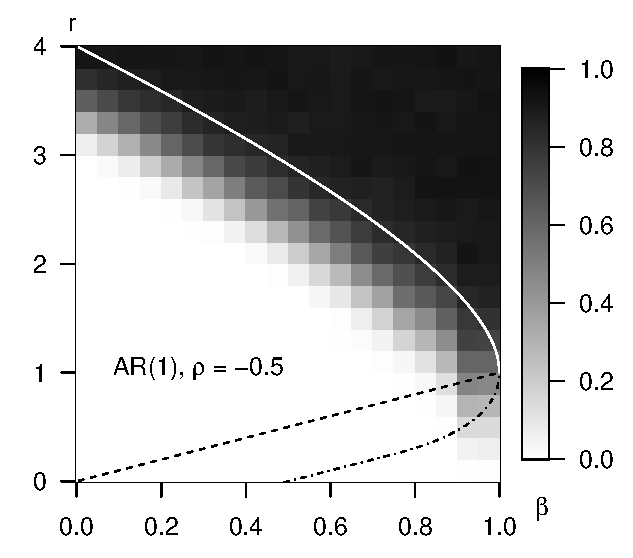
\includegraphics[width=0.4\textwidth]{./figures/simulated_phase_diagram_AR-05_p10000.eps}
    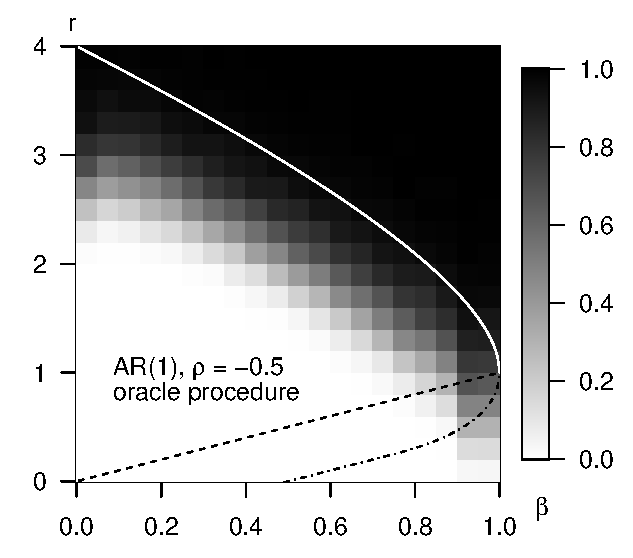
\includegraphics[width=0.4\textwidth]{./figures/simulated_phase_diagram_AR-05_p10000_oracle.eps}
    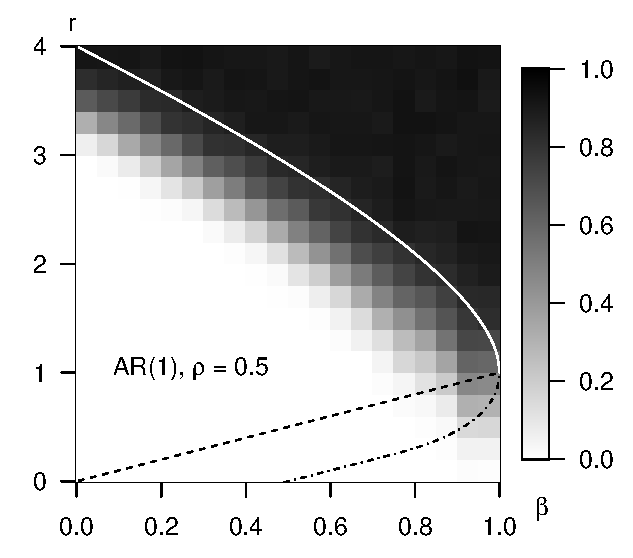
\includegraphics[width=0.4\textwidth]{./figures/simulated_phase_diagram_AR05_p10000.eps}
    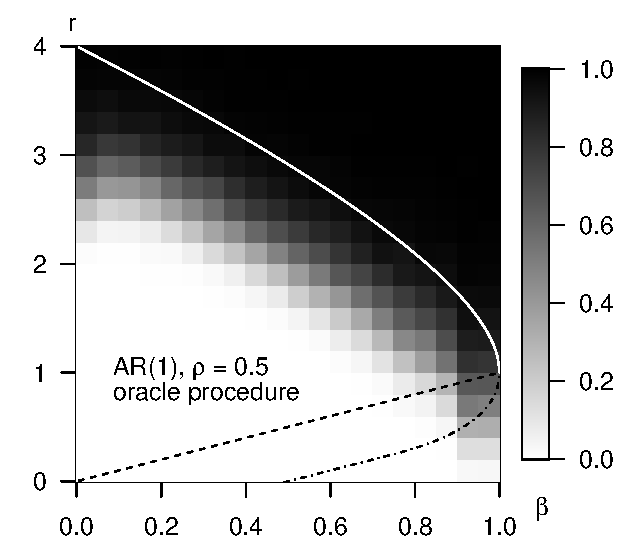
\includegraphics[width=0.4\textwidth]{./figures/simulated_phase_diagram_AR05_p10000_oracle.eps}
    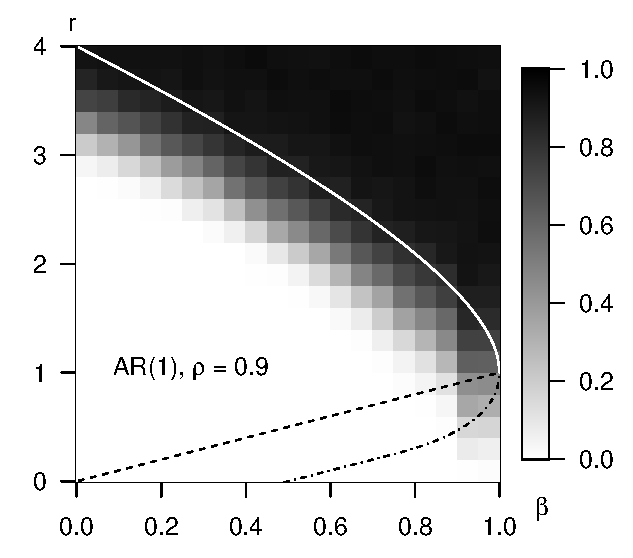
\includegraphics[width=0.4\textwidth]{./figures/simulated_phase_diagram_AR09_p10000.eps}
    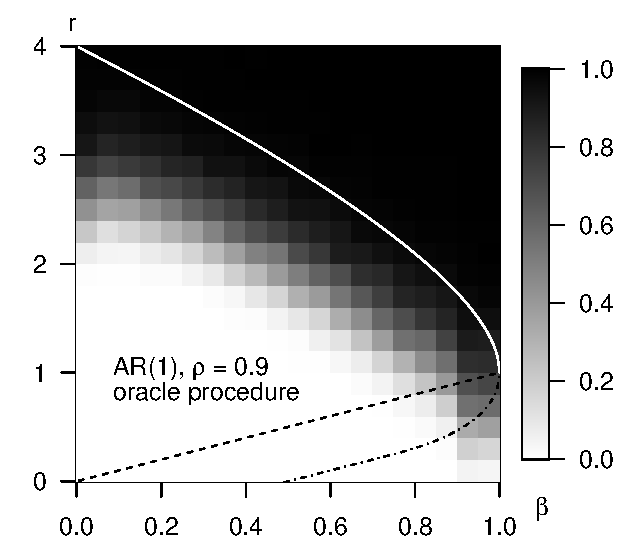
\includegraphics[width=0.4\textwidth]{./figures/simulated_phase_diagram_AR09_p10000_oracle.eps}
    \caption{The empirical probability of exact support recovery from numerical experiments, as a function of sparsity level $\beta$ and signal sizes $r$. Darker colors indicate higher probability of exact support recovery. 
    Three AR(1) models with autocorrelation functions $(-0.5)^k$ (upper), 
    $0.5^k$ (middle), and $0.9^k$ (lower) are simulated.
    The experiments were repeated 1000 times for each sparsity-signal size combination.
    In finite dimensions ($p=10000$), the Bonferroni procedures (left) suffers small loss of power compared to the oracle procedures (right).
    A phase transition in agreement with the predicted boundary \eqref{eq:strong-classification-boundary} can be seen in the AR models.
    The boundaries (solid, dashed, and dash-dotted lines) are as in Fig \ref{fig:phase-simulated}.}
    \label{fig:phase-simulated-dependent}
\end{figure}

\medskip

The second set of experiments explores exact support recovery in additive error models in the cases of long-range dependent but UDD, as well as non-UDD errors.
In particular we simulate
\begin{itemize}
    \item Fractional Gaussian noise (fGn) with Hurst parameter $H = 0.75$ and $H = 0.9$. 
    The autocovariance functions are 
    % $$\rho_{k} \sim 2H(2H-1)k^{2H-2},$$
    $$\rho_{k} \sim 0.75k^{-0.6} \quad \text{and} \quad \rho_{k} \sim 1.44k^{-0.2},$$
    as $k\to\infty$.
    Both fGn models represent the regime of long-range dependence, where covariances decay very slowly to zero, so that $\sum|\rho_k| = \infty$; see, e.g., \citep{taqqu2003livre}.
    Observe that every stationary Gaussian process with vanishing autocovariance gives rise to an UDD array as concluded in Corollary \ref{cor:stationary-Gaussian-errors}.
    \item The non-UDD Gaussian errors described in Example \ref{exmp:counter-example}.
\end{itemize}
We will apply both the sparsity-and-signal-size-agnostic Bonferroni's procedure, i.e., $\widetilde{S} = \{i:x(i)>\sqrt{2\log{p}}\}$, as well as the oracle procedure $\widehat{S}^* = \{i:x(i)\ge x_{[s]}\}$, $s=|S|$, to all settings.
Results of the numerical experiments for the fGn and non-UDD models are shown in Figure \ref{fig:phase-simulated-very-dependent}.


\begin{figure}
    \centering
    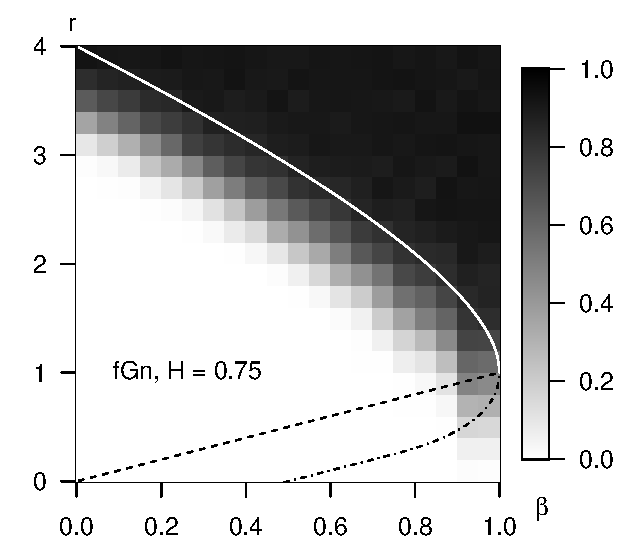
\includegraphics[width=0.4\textwidth]{./figures/simulated_phase_diagram_fGn075_p10000.eps}
    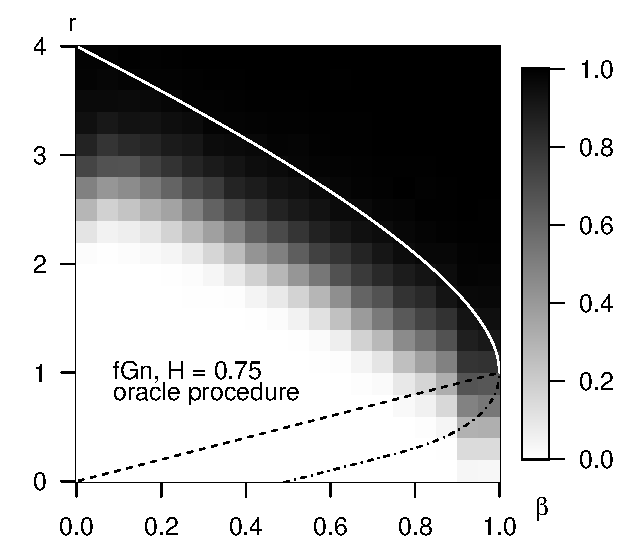
\includegraphics[width=0.4\textwidth]{./figures/simulated_phase_diagram_fGn075_p10000_oracle.eps}
    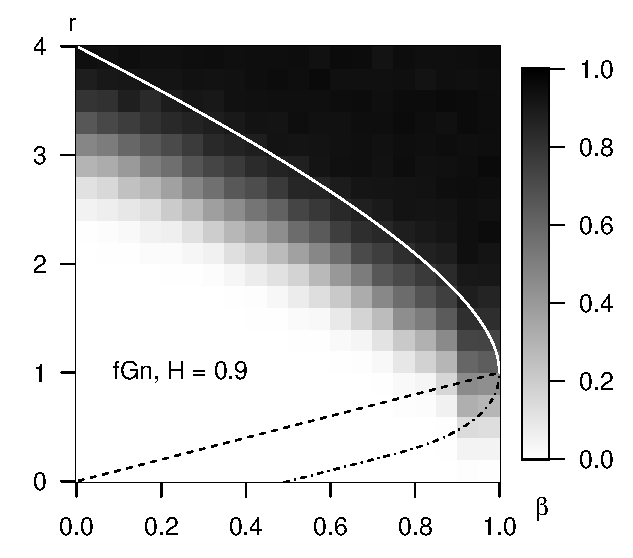
\includegraphics[width=0.4\textwidth]{./figures/simulated_phase_diagram_fGn09_p10000.eps}
    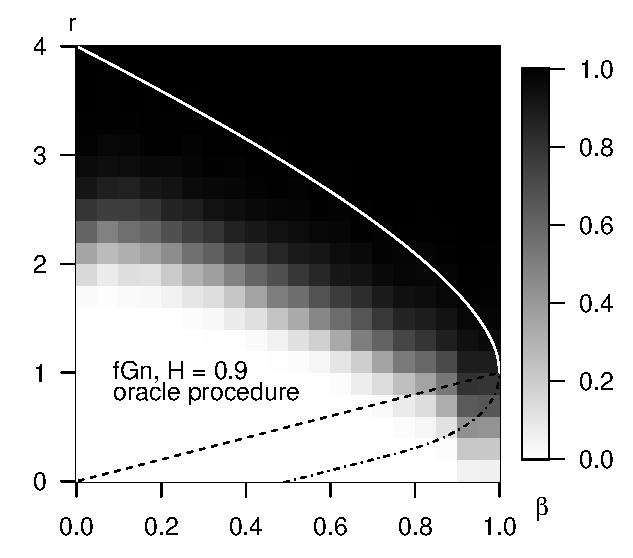
\includegraphics[width=0.4\textwidth]{./figures/simulated_phase_diagram_fGn09_p10000_oracle.eps}
    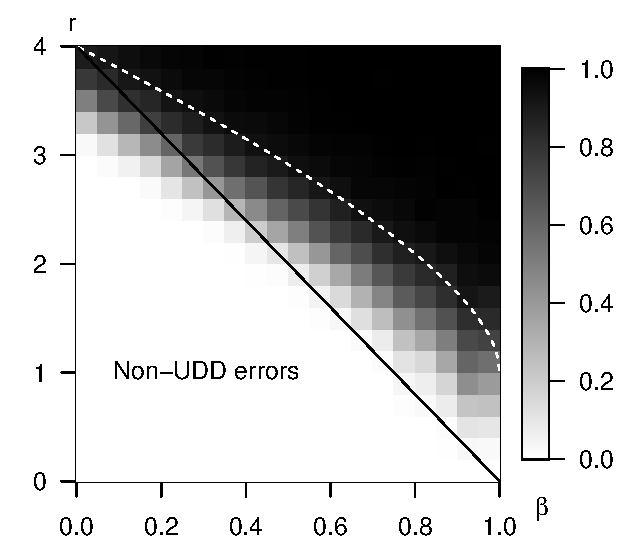
\includegraphics[width=0.4\textwidth]{./figures/simulated_phase_diagram_block_structure_p10000_agnostic7.eps}
    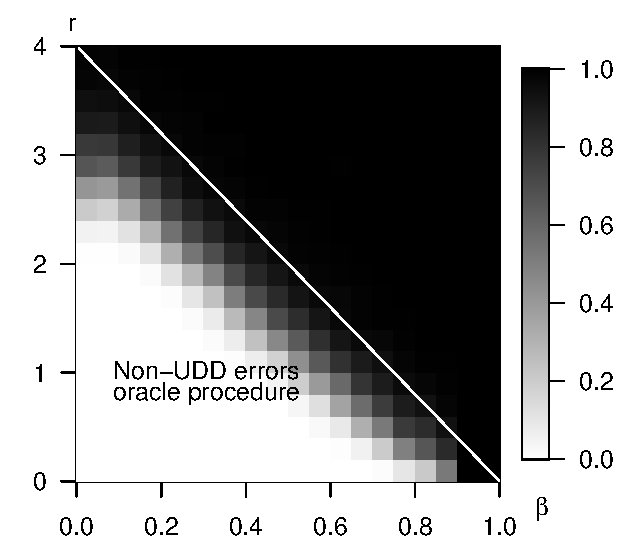
\includegraphics[width=0.4\textwidth]{./figures/simulated_phase_diagram_block_structure_p10000_oracle6.eps}
    \caption{The empirical probability of exact support recovery from numerical experiments, as a function of sparsity level $\beta$ and signal sizes $r$. Darker colors indicate higher probability of exact support recovery. 
    Two fGn models with Hurst parameter $H = 0.75$ (upper), 
    $H = 0.9$ (middle), and the non-UDD errors in Example \ref{exmp:counter-example} (lower) are simulated.
    The experiments were repeated 1000 times for each sparsity-signal size combination.
    In finite dimensions ($p=10000$), the oracle procedures (right) is able to recover support for weaker signals than the Bonferroni procedures (left) when errors are heavily dependent, although they have the same phase transition limit.
    The non-UDD errors demonstrate qualitatively different behavior, enabling support recovery for strictly weaker signals.
    The boundaries (solid, dashed, and dash-dotted lines) are as in Fig \ref{fig:phase-simulated}.
    In the non-UDD example, dashed lines represent the limit attained by Bonferroni's procedures.
    See text for additional comments.}
    \label{fig:phase-simulated-very-dependent}
\end{figure}


Notice that the oracle procedure sets its thresholds more aggressively (at roughly $\sqrt{2\log s}$) than the Bonferroni procedure (at $\sqrt{2\log p}$).
Although this difference vanishes as $p\to\infty$, in finite dimensions ($p=10\,000$) the advantage can be felt. 
Indeed, in all our experiments the oracle procedure is able to recover support of signals with higher probability than the Bonferroni procedures; compare left and right columns of Figure  \ref{fig:phase-simulated-very-dependent}.
Notice also that there is an increase in probability of recovery near $\beta=0$ for oracle procedures.
This is an artifact in finite dimensions due to the fact that $s = \lfloor p^{1-\beta}\rfloor < p/2$, and there are more signals than nulls. The oracle procedures is able to adjust to this reversal by lowering its threshold accordingly.

For UDD errors, Theorem \ref{thm:necessary} predicts that exact recovery of the support is impossible when signal sizes are below the boundary \eqref{eq:strong-classification-boundary}, even with oracle procedures. 
% Both the AR and the fGn models generate UDD Gaussian errors, and should demonstrate the same phase-transition boundary.
However, the rate of this convergence (i.e., $\P[\widehat{S}^*=S]\to0\;\text{or}\;1$) can be very slow when the errors are heavily dependent,
even though all AR and fGn models demonstrate qualitatively the same behavior in line with the predicted boundary \eqref{eq:strong-classification-boundary}. 
In finite dimensions ($p=10\,000$), as dependence in the errors increases (fGN(H=0.75) to fGN(H=0.9)), the oracle procedure becomes more powerful at recovering signal support with high probability for weaker signals. 

On the other hand, as demonstrated in Example \ref{exmp:counter-example}, non-UDD errors yield qualitatively different behavior; exact support recovery is possible for signal sizes strictly weaker than that in the UDD case. 
Lower-right panel of Figure \ref{fig:phase-simulated-very-dependent} demonstrates in this example that the signal support can be recovered as long as the signal sizes are larger than $4(1-\beta)$.





\chapter{\comment{The Phase Transition Phenomena in}
Fundamental Statistical Limits in Genome-wide Association Studies} 
\label{chap:GWAS}

We investigate the fundamental limits of multiple testing problems in high-dimensional chi-square models, and in genome-wide association studies as introduced in Section \ref{sec:motivation-chisq}.

In Section \ref{sec:chisq-boundaries}, we shall establish the phase transitions of the sparse chi-square model \eqref{eq:model-chisq}.
Recall that in large-scale screening studies where a large number of association tests are conducted, resulting statistics may be approximated by
\begin{equation} \label{eq:model-chisq-Chapter6}
    %x(i) \distras{\mathrm{ind.}} \chi_\nu^2\left(\lambda(i)\right), \quad i=1,\ldots,p.
    x(i) \sim \chi_\nu^2\left(\lambda(i)\right), \quad i=1,\ldots,p,
\end{equation}
where $\chi_\nu^2\left(\lambda(i)\right)$ is a chi-square distributed random variable with $\nu$ degrees of freedom and non-centrality parameter $\lambda(i)$.
In parallel to results in Chapter \ref{chap:phase-transitions}, we show that several commonly used family-wise error rate-control procedures --- including Bonferroni's procedure --- are asymptotically optimal for the {exact}, and {exact-approximate} support recovery problems (as defined in Definition \ref{def:exact-recovery-success-failure}) in idealized chi-square models \eqref{eq:model-chisq-Chapter6} with independent components.
We further show that the \ac{BH} procedure is asymptotically optimal for the {approximate}, and {approximate-exact} support recovery problems.
% \ref{thm:chi-squared-exact-boundary}, \ref{thm:chi-squared-exact-approx-boundary}, \ref{thm:chi-squared-approx-boundary}, and \ref{thm:chi-squared-approx-exact-boundary}.
Under appropriate parametrizations of the signal sizes and sparsity, they establish the phase transitions of support recovery problems in the chi-square model.
Remarkably, the degree-of-freedom parameter does not affect the asymptotic boundaries in any of the four support recovery problems.

All phase transition boundaries coincide with those in the additive error models obtained in Chapter \ref{chap:phase-transitions} under suitable parametrizations.
% and Figure \ref{fig:phase-chi-squared} continues to apply.
indicating vanishing differences between the difficulties of the one-sided and two-sided alternatives in the Gaussian additive error model \eqref{eq:model-additive}.

\medskip

We then return to association screenings of categorical variables in
Section \ref{sec:odds-and-power}, and present the consequences of the phase transition in the exact-approximate problem in large-scale genetic association studies.
% present empirical evidence for the phase transition in the exact-approximate problem using real data from large-scale association studies on breast cancer obtained from the NHGRI-EBI GWAS Catalog \citep{macarthur2016new}.
% demystify the notion of signal size $\lambda$ in this context.
% which is perhaps less transparent than in additive error models.
We do so by characterizing the relationship between the signal size $\lambda$ and the marginal frequencies, odds ratio, and sample sizes for association tests on 2-by-2 contingency tables.
% Specifically, the amount of signal, when rare variants are present, is weaker compared to the signal when the marginal distributions are balanced.
% In other words, reliable detection of the effects by rare variants would require more samples compared to common variants, even at the same odds ratio.
This result, establishing the relationship between sample sizes and signal sizes, is made precise in Section \ref{sec:odds-and-power}.

We elaborate on the implications of this relationship on optimal study designs for association studies in Section \ref{sec:optimal-design}.
Perhaps surprisingly, our analysis reveals that balanced designs with equal number of cases and controls are often statistically inefficient.
Practical consequences of these results in power analysis will be illustrated with data examples in Section \ref{sec:phase-transitions-in-GWAS}. 

The phase transitions in the chi-square models are demonstrated with numerical simulations in Section \ref{sec:numerical}.
Proofs of results in this Chapter are collected in Section \ref{sec:proof-signal-size-odds-ratio}.

% Practical issues are also addressed to make for simple and effective power analysis.

\section{Support recovery problems in chi-squared models}
\label{sec:chisq-boundaries}

Similar to the analysis of additive error models in Chapter \ref{chap:phase-transitions}, we will work with triangular arrays of chi-square models \eqref{eq:model-chisq-Chapter6} indexed by $p$.
We adopt the same parametrization for the sparsity of the non-centrality parameter vectors $\lambda = \lambda_p$,
\begin{equation} \label{eq:signal-sparsity}
    |S_p| = \left\lfloor p^{1-\beta} \right\rfloor, \quad \beta\in(0,1]
\end{equation}
where $\beta$ parametrizes the problem sparsity.
The closer $\beta$ is to 1, the sparser the support $S_p$; conversely, when $\beta$ is close to 0, the support is dense with many non-null signals.

We parametrize the range of the non-zero and perhaps unequal signals in the chi-square model with
\begin{equation} \label{eq:signal-size}
    \underline{\Delta} = 2\underline{r}\log{p}
    \le \lambda(i) \le
    \overline{\Delta} = 2\overline{r}\log{p}, \quad \text{for all}\;\;i\in S_p,
\end{equation}
for some constants $0<\underline{r}\le\overline{r}\le+\infty$.

\subsection{The exact support recovery problem}
\label{subsec:exact-support-recovery-chisq}

The first main result characterizes the phase transition phenomenon in the exact support recovery problem under the chi-square model.

\begin{theorem} \label{thm:chi-squared-exact-boundary}
Consider the high-dimensional chi-squared model \eqref{eq:model-chisq-Chapter6} with signal sparsity and size as described in \eqref{eq:signal-sparsity} and \eqref{eq:signal-size}.
The function 
\begin{equation} \label{eq:exact-boundary-chisquared}
    g(\beta) = \left(1 + \sqrt{1-\beta}\right)^2
\end{equation}
characterizes the phase transition of exact support recovery problem.
Specifically, if $\underline{r} > {{g}}(\beta)$, then Bonferroni's, Sid\'ak's, Holm's, and Hochberg's procedures with slowly vanishing (see Definition \ref{def:slowly-vanishing}) nominal FWER levels all achieve asymptotically exact support recovery in the sense of \eqref{eq:support-recovery-success}. 

Conversely, if $\overline{r} < {{g}}(\beta)$, then for any thresholding procedure $\widehat{S}_p$, we have $\P[\widehat{S}_p=S_p]\to0$.
Therefore, in view of Lemma \ref{lemma:risk-exact-recovery-probability}, exact support recovery asymptotically fails for all thresholding procedures in the sense of \eqref{eq:support-recovery-failure}.
\end{theorem}

% \begin{figure}
%   \begin{center}
%     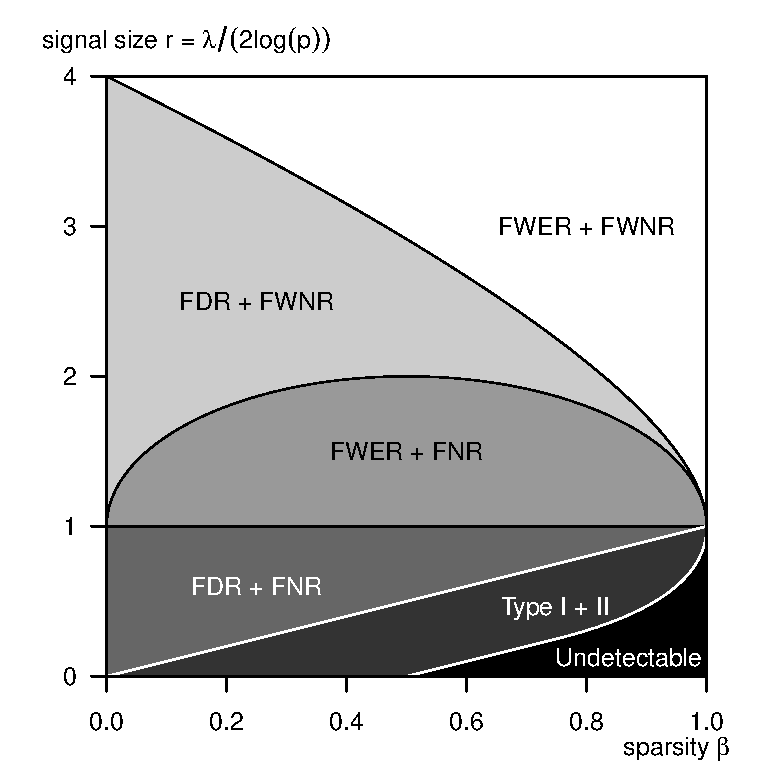
\includegraphics[width=0.7\textwidth]{./pics/phase_diagram_chisquared_ALL_boundaries.eps}
%   \end{center}
%    \caption{The phase diagram for the high-dimensional chi-square model \eqref{eq:model-chisq}, illustrating the boundaries of the exact support recovery (FWER + FWNR; top curve; Theorem \ref{thm:chi-squared-exact-boundary}), the approximate-exact support recovery (FDR + FWNR; second curve from top; Theorem \ref{thm:chi-squared-approx-exact-boundary}), the exact-approximate support recovery (FWER + FNR; horizontal line $r=1$; Theorem \ref{thm:chi-squared-exact-approx-boundary}), and the approximate support recovery problems (FDR + FNR; tilted line $r=\beta$; Theorem \ref{thm:chi-squared-approx-boundary}). The signal detection problem (type I + type II errors of the global test; lower curve) was studied in Donoho and Jin (2004). In each region of the diagram and above, the annotated statistical risk can be made to vanish, as dimension $p$ diverges. Conversely, the risks has liminf at least one. All boundaries are unaffected by the degree-of-freedom. All boundaries are identical to those in the Gaussian additive error model \eqref{eq:model-additive} under one-side alternatives; c.f., results in Section \ref{sec:additive-error-model-boundaries}.}
%    \label{fig:phase-chi-squared}
% \end{figure}


The procedures listed in Theorem \ref{thm:chi-squared-exact-boundary} were reviewed in Section \ref{sec:statistical-procedures}. 
Proof of the theorem can be found in Section \ref{subsec:proof-chi-squared-exact-boundary}. 
% The boundary \eqref{eq:exact-boundary-chisquared} is plotted in Figure \ref{fig:phase-chi-squared}.

It is evident that the exact support recovery boundary \eqref{eq:exact-boundary-chisquared} coincides with that in parallel results for the Gaussian additive error models \eqref{eq:model-additive} in Chapter \ref{chap:phase-transitions}.
Implications of these results will be discussed in Section \ref{subsec:one-vs-two-sided} below.

\begin{remark} \label{rmk:strong-classification-boundary-2}
Theorem \ref{thm:chi-squared-exact-boundary} predicts that the asymptotic boundaries are the same for all values of the parameter $\nu$.
In simulations (Section \ref{sec:numerical}), we find this asymptotic prediction to be quite accurate for $\nu\le3$ even in moderate dimensions ($p=100$). 
For $\nu>3$, the phase transitions take place somewhat above the boundary ${g}$.
The behavior is qualitatively similar for the other three phase transitions (see Theorems \ref{thm:chi-squared-exact-approx-boundary}, \ref{thm:chi-squared-approx-boundary}, and \ref{thm:chi-squared-approx-exact-boundary} below).
\end{remark}

\subsection{The exact-approximate support recovery problem}
\label{subsec:exact-approx-support-recovery-chisq}

The next theorem describes the phase transition in the exact-approximate support recovery problem.

\begin{theorem} \label{thm:chi-squared-exact-approx-boundary}
In the context of Theorem \ref{thm:chi-squared-exact-boundary}, 
the function 
\begin{equation} \label{eq:exact-approx-boundary-chisquared}
    \widetilde{g}(\beta) = 1
\end{equation}
characterizes the phase transition of exact-approximate support recovery problem.
Specifically, if $\underline{r} > \widetilde{g}(\beta)$, then the procedures listed in Theorem \ref{thm:chi-squared-exact-boundary} with slowly vanishing nominal FWER levels achieve asymptotically exact-approximate support recovery in the sense of \eqref{eq:support-recovery-success}. 

Conversely, if $\overline{r} < \widetilde{g}(\beta)$, then for any thresholding procedure $\widehat{S}_p$, the exact-approximate support recovery fails in the sense of \eqref{eq:support-recovery-failure}.
\end{theorem}

Theorem \ref{thm:chi-squared-exact-approx-boundary} is proved in Section \ref{subsec:proof-chi-squared-mix-boundaries}. 


\subsection{The approximate support recovery problem}
\label{subsec:approx-support-recovery-chisq}

Our third main result characterizes the phase transition phenomenon in the approximate support recovery problem in the chi-square model.

\begin{theorem} \label{thm:chi-squared-approx-boundary}
Consider the high-dimensional chi-squared model \eqref{eq:model-chisq-Chapter6} with signal sparsity and size as described in \eqref{eq:signal-sparsity} and \eqref{eq:signal-size}.
The function 
\begin{equation} \label{eq:approx-boundary-chisquared}
    h(\beta) = \beta
\end{equation}
characterizes the phase transition of approximate support recovery problem.
Specifically, if $\underline{r} > {h}(\beta)$, then the \ac{BH} procedure $\widehat{S}_p$ (defined in Section \ref{sec:statistical-procedures}) with slowly vanishing (see Definition \ref{def:slowly-vanishing}) nominal FDR levels achieves asymptotically approximate support recovery in the sense of \eqref{eq:support-recovery-success}. 

Conversely, if $\overline{r} < {h}(\beta)$, then approximate support recovery asymptotically fails in the sense of \eqref{eq:support-recovery-failure} for all thresholding procedures.
\end{theorem}

Theorem \ref{thm:chi-squared-approx-boundary} is proved in Section \ref{subsec:proof-chi-squared-mix-boundaries} below. 


\subsection{The approximate-exact support recovery problem}
\label{subsec:aprox-exact-support-recovery-chisq}

A counterpart of Theorem \ref{thm:Gaussian-error-approx-exact-boundary} also holds in the chi-square models.

\begin{theorem} \label{thm:chi-squared-approx-exact-boundary}
In the context of Theorem \ref{thm:chi-squared-approx-boundary}, the function 
\begin{equation} \label{eq:approx-exact-boundary-chisquared}
    \widetilde{h}(\beta) = \left(\sqrt{\beta} + \sqrt{1-\beta}\right)^2
\end{equation}
characterizes the phase transition of approximate-exact support recovery problem.
Specifically, if $\underline{r} > \widetilde{h}(\beta)$, then the Benjamini-Hochberg procedure with slowly vanishing nominal FDR levels achieves asymptotically approximate-exact support recovery in the sense of \eqref{eq:support-recovery-success}. 

Conversely, if $\overline{r} < \widetilde{h}(\beta)$, then for any thresholding procedure $\widehat{S}_p$, the approximate-exact support recovery fails in the sense of \eqref{eq:support-recovery-failure}.
\end{theorem}

Theorem \ref{thm:chi-squared-approx-exact-boundary} is proved in Section \ref{subsec:proof-chi-squared-exact-boundary}. 

Notice that all phase transitions boundaries are identical to those in the Gaussian additive error model \eqref{eq:model-additive} under one-side alternative.
We refer readers to Figure \ref{fig:phase-Gaussian-errors} in Section \ref{sec:additive-error-model-boundaries} for a visualization of the results in Theorems \ref{thm:chi-squared-exact-boundary} through \ref{thm:chi-squared-approx-exact-boundary}.

\medskip

The all four Theorems so far focus only on the idealized models \eqref{eq:model-chisq-Chapter6} where statistics are \emph{independent}.
Support recovery problems under dependent observations remain to be explored.
Recall in Chapter \ref{chap:phase-transitions} we showed that the boundary for the exact support recovery problem in the additive error model \eqref{eq:model-additive} continues to hold even under severe dependence and general distributional assumptions.
We conjecture that similar results would also hold, under classes of dependence structures that are ``not too different from independence'', in the chi-square models.
As an example, in the GWAS application, dependence among the genetic markers at different locations (known as linkage disequilibrium) decay as a function of their physical distances on the genome \citep{bush2012genome}, resulting in locally dependent test statistics.
It would be of great interest to extend the current theory to cover important dependence structures that arise in such applications.


\subsection{Comparison of one- versus two-sided alternatives in additive error models}
\label{subsec:one-vs-two-sided}


% $\mathrm{risk}^{\mathrm{EA}}$ and $\mathrm{risk}^{\mathrm{AE}}$.
As alluded to in Section \ref{sec:motivation-chisq} in the introduction, we draw explicit comparisons between the one-sided and two-sided alternatives in Gaussian additive error models \eqref{eq:model-additive}.
% The exact, and the approximate support recovery problems in the additive error model \eqref{eq:model-additive} under standard Gaussian errors have been studied in \cite{gao2018fundamental} and \cite{arias2017distribution}, respectively. 

The exact support recovery problem in the dependent Gaussian additive error model \eqref{eq:model-additive} was studied in Chapter \ref{chap:phase-transitions}, with parametrization of sparsity identical to that in \eqref{eq:signal-sparsity}, whereas the range of the non-zero (and perhaps unequal) mean shifts $\mu(i)$ was parametrized as 
\begin{equation*}
    \underline{\Delta} = \sqrt{2\underline{r}\log{p}}
    \le \mu(i) \le
    \overline{\Delta} = \sqrt{2\overline{r}\log{p}}, \quad \text{for all}\;\;i\in S_p,
\end{equation*}
for some constants $0<\underline{r}\le\overline{r}\le+\infty$.
Under this one-sided alternative, a phase transition in the $r$-$\beta$ plane was described, where the boundary was found to be identical to \eqref{eq:exact-boundary-chisquared} in Theorem \ref{thm:chi-squared-exact-boundary} for the chi-square models \eqref{eq:model-chisq-Chapter6}. 

As discussed in Section \ref{sec:motivation-chisq}, support recovery problems in the chi-square model with $\nu=1$ correspond to the support recovery problems in 
the additive model under two-sided alternatives. This implies that the asymptotic signal size requirements are identical between the two-sided alternative and its 
one-sided counterpart, in order to achieve exact support recovery. As we shall see in numerical experiments (in Section \ref{sec:numerical} below), the difference 
is not very pronounced even in moderate dimensions, and vanishes as $p\to\infty$, in accordance with Theorem \ref{thm:chi-squared-exact-boundary}.

\medskip

Comparisons can also be drawn in the approximate, approximate-exact, and exact approximate support recovery problems between the two types of alternatives.

Specifically, the approximate support recovery problem in the Gaussian additive error model \eqref{eq:model-additive} under one-sided alternatives exhibits a phase transition phenomenon characterized by a boundary that coincides with \eqref{eq:approx-boundary-chisquared} in Theorem \ref{thm:chi-squared-approx-boundary}.
Similar to the exact support recovery problem, this indicates vanishing difference in the difficulties of the two types alternatives in approximate support recovery problems.

Comparing Theorems \ref{thm:chi-squared-exact-approx-boundary} to \ref{thm:Gaussian-error-exact-approx-boundary} and Theorems \ref{thm:chi-squared-approx-exact-boundary} to \ref{thm:Gaussian-error-approx-exact-boundary}, we see that the phase transition boundaries under the two types of alternatives are also identical in the exact-approximate and approximate-exact support recovery problems.

To complete the comparisons, we point out that the phase transition boundaries for the sparse signal {detection} problem in the two types of alternatives are both identical to \eqref{eq:detection-boundary-large-signals}. This was analyzed in \cite{donoho2004higher}.

Therefore, all phase transition boundaries coincide with those in the additive error models obtained in Chapter \ref{chap:phase-transitions} under their respective parametrizations.
% and Figure \ref{fig:phase-chi-squared} continues to apply.
This indicates vanishing differences between the difficulties of the one-sided and two-sided alternatives in the Gaussian additive error model \eqref{eq:model-additive}.
The additional uncertainty in the two-sided alternatives do not call for larger signal sizes in these problems, asymptotically.





\section{Odds ratios and statistical power}
\label{sec:odds-and-power}

We return to the application of association screenings for categorical variables, and put the results in the previous section to use.
In particular, we focus on the exact-approximate support recovery problem, and demonstrate the consequences of its phase transition (Theorem \ref{thm:chi-squared-exact-approx-boundary}) in genetic association studies.

In order to do so, we must first connect the concept of ``statistical signal size'' $\lambda$ with some key quantities in association tests.
While ``signal size'' likely sounds foreign to most practitioners, it is intimately linked with the concept of ``effect sizes'' --- or odds ratios --- in association studies, which are frequently estimated and reported in GWAS catalogs.
We characterize the relationship between the two quantities in the special, but fairly common case of association tests on 2-by-2 contingency tables in Section \ref{sec:odds-and-power}.

% Unlike in additive models where the parameter $\mu$ has the interpretation of signal-to-noise ratios, the meaning of the signal sizes $\lambda$ in chi-square model is perhaps not as transparent.

Consider a 2-by-2 multinomial distribution with marginal probabilities of phenotypes $(\phi_1, \phi_2)$ and genotypes $(\theta_1, \theta_2)$.
The \emph{probability} table (as opposed to the table of multinomial \emph{counts} in the introduction) is as follows.
\begin{center}
    \begin{tabular}{cccc}
    \hline
    & \multicolumn{2}{c}{Genotype} \\
    \cline{2-3}
    Probabilities & Variant 1 & Variant 2 & Total by phenotype \\
    \hline
    Cases & $\mu_{11}$ & $\mu_{12}$ & $\phi_1$ \\
    Controls & $\mu_{21}$ & $\mu_{22}$ & $\phi_2$ \\
    Total by genotype & $\theta_1$ & $\theta_2$ & 1 \\
    \hline
    \end{tabular}
\end{center}
The odds ratio (i.e., ``effect size'') is defined as the ratio of the phenotype frequencies between the two genotype variants,
\begin{equation} \label{eq:odds-ratio}
    \text{R} := \frac{\mu_{11}}{\mu_{21}}\Big/\frac{\mu_{12}}{\mu_{22}}
    = \frac{\mu_{11}\mu_{22}}{\mu_{12}\mu_{21}}.
\end{equation}
The multinomial distribution is fully parametrized by the trio $(\theta_1, \phi_1, R)$.
Odds ratios further away from 1 indicate greater contrasts between the probability of outcomes.
Independence between the genotypes and phenotypes would imply an odds ratio of one, and hence $\mu_{jk} = \phi_j\theta_k$, for all $j,k \in\{1,2\}$.

% When data are sampled from the multinomial distribution, the chi-square test defined in \eqref{eq:chisq-statistic} is asymptotically equivalent to tests including, e.g., the likelihood ratio test and Welch's t-test, both in terms of level and power \cite{ferguson2017course,gao2019upass}.
For a sequence of local alternatives $\mu^{(1)}, \mu^{(2)}, \ldots$, such that $\sqrt{n}(\mu^{(n)}_{jk} - \phi_j\theta_k)$ converges to a constant table $\delta = (\delta_{jk})$, the chi-square test statistics converge in distribution to the non-central chi-squared distribution with non-centrality parameter 
\begin{equation*}
    \lambda = \sum_{j=1}^2 \sum_{k=1}^2 {\delta_{jk}^2}/{(\phi_j\theta_k)}.
\end{equation*}
See, e.g., \cite{ferguson2017course}.
Hence, for large samples from a fixed distribution $(\mu_{ij})$, the statistic is well approximated by a $\chi^2_1(\lambda)$ distribution, where
\begin{equation} 
\lambda = n\sum_{j=1}^2 \sum_{k=1}^2 \frac{(\mu_{jk} - \phi_j\theta_k)^2}{\phi_j\theta_k}.
\end{equation}
%Since $\lambda$ is linear in the number of samples $n$, 
% Power of association tests at $\alpha$ level is approximately $\P[\chi^2_{\nu}(\lambda)>\chi^2_{\nu,\alpha}]$, where $\chi^2_{\nu,\alpha}$ is the upper $\alpha$-quantile of a central Chi-squared distribution.
Power calculations therefore only depend on the $\mu_{jk}$'s through $\lambda=nw^2$, where we define 
\begin{equation} \label{eq:signal-size-chisq}
    w^2:=\lambda/n
\end{equation} 
to be the \emph{signal size per sample}. 
Statistical power would be increasing in $w^2$ for fixed sample sizes.

The next proposition states that the statistical signal size per sample can be parametrized by the odds ratio and the marginals in the probability table.

\begin{proposition} \label{prop:signal-size-odds-ratio}
Consider a 2-by-2 multinomial distribution with marginal distributions $(\phi_1, \phi_2 = 1-\phi_2)$ and $(\theta_1, \theta_2=1-\theta_1)$.
Let signal size $w^2$ be defined as in \eqref{eq:signal-size-chisq}, and odds ratio $\text{R}$ be defined as in \eqref{eq:odds-ratio}. 
If $R=1$, we have $w^2 = 0$; if $R\in(0,1)\cup(1,+\infty)$, then we have
\begin{equation} \label{eq:signal-size-odds-ratio}
    w^2(\text{R}) =
    \frac{1}{4A(\text{R}-1)^2}\left(B+CR-\sqrt{(B+CR)^2-4A(R-1)^2}\right)^2,
\end{equation}
where $A = \phi_1\theta_1\phi_2\theta_2$, $B = \phi_1\theta_1+\phi_2\theta_2$, and $C = \phi_1\theta_2+\phi_2\theta_1$.
\end{proposition}

\begin{proof}
	We parametrize the 2-by-2 multinomial distribution with the parameter $\delta$, 
	\begin{equation} \label{eq:reparametrize-2-by-2-table-1}
	\mu_{11} = \phi_1\theta_1+\delta,\quad 
	\mu_{12} = \phi_1\theta_2-\delta,\quad 
	\mu_{21} = \phi_2\theta_1-\delta,\quad 
	\mu_{22} = \phi_2\theta_2+\delta.
	\end{equation}
	By relabelling of categories, we may assume $0<\theta_1,\phi_1\le1/2$ without loss of generality.
	Note that $\delta$ must lie within the range $[\delta_\mathrm{min}, \delta_\mathrm{max}]$, where
	$$
	\delta_\mathrm{min} := \max\{-\phi_1\theta_1, -\phi_2\theta_2, \phi_1\theta_2-1, \phi_2\theta_1-1\} 
	= -\phi_1\theta_1,
	$$
	and
	$$
	\delta_\mathrm{max} := \min\{1-\phi_1\theta_1, 1-\phi_2\theta_2, \phi_1\theta_2, \phi_2\theta_1\}
	= \min\{\phi_1\theta_2, \phi_2\theta_1\},
	$$
	in order for $\mu_{ij}\ge0$ for all $i,j\in \{1,2\}$.
	Under this parametrization, Relation \eqref{eq:odds-ratio} then becomes
	\begin{equation} \label{eq:odds-ratio-delta}
	\text{R} = \frac{\mu_{11}\mu_{22}}{\mu_{12}\mu_{21}}
	= \frac{\phi_1\theta_1\phi_2\theta_2 + \delta(\phi_1\theta_1+\phi_2\theta_2)+\delta^2}{\phi_1\theta_1\phi_2\theta_2 - \delta(\phi_1\theta_2+\phi_2\theta_1)+\delta^2},
	\end{equation}
	which is one-to-one and increasing in $\delta$ on $(\delta_\mathrm{min}, \delta_\mathrm{max})$.
	Equation \eqref{eq:signal-size-chisq} becomes
	\begin{equation} \label{eq:signal-size-chisq-delta}
	w^2 = \sum_{i=1}^2 \sum_{j=1}^2 \frac{(\mu_{ij} - \phi_i\theta_j)^2}{\phi_i\theta_j}
	= \delta^2\sum_i\sum_j \frac{1}{\phi_i\theta_j}
	= \frac{\delta^2}{\phi_1\theta_1\phi_2\theta_2},
	\end{equation}
	Solving for $\delta$ in \eqref{eq:odds-ratio-delta}, and plugging into the expression for signal size \eqref{eq:signal-size-chisq-delta} yields Relation \eqref{eq:signal-size-odds-ratio}.
	
	The other three cases ($1/2\le\theta_1,\phi_1\le1$; $0<\theta_1\le1/2\le\phi_1\le1$; and $0\le\phi_1\le1/2\le\theta_1\le1$) may be obtained similarly, or by appealing to the symmetry of the problem.
\end{proof}

To understand Proposition \ref{prop:signal-size-odds-ratio}, we illustrate Relation \eqref{eq:signal-size-odds-ratio} for selected values of marginals $\theta_1$ and $\phi_1$ in Figure \ref{fig:signal-vs-odds}.
Observe in the figure that an odds ratio further away from one corresponds to stronger statistical signal per sample, ceteris paribus.
However, this ``valley'' pattern is in general not symmetric around 1, except for balanced marginal distributions ($\phi_1=1/2$ or $\theta_1=1/2$).
While the odds ratio $R$ can be arbitrarily close to 0 or diverge to $+\infty$ for any marginal distribution, the signal sizes $w^2$ are bounded from above by constants that depend only on the marginals.
% This is quantified in the next corollary.

\begin{figure}
      \centering
      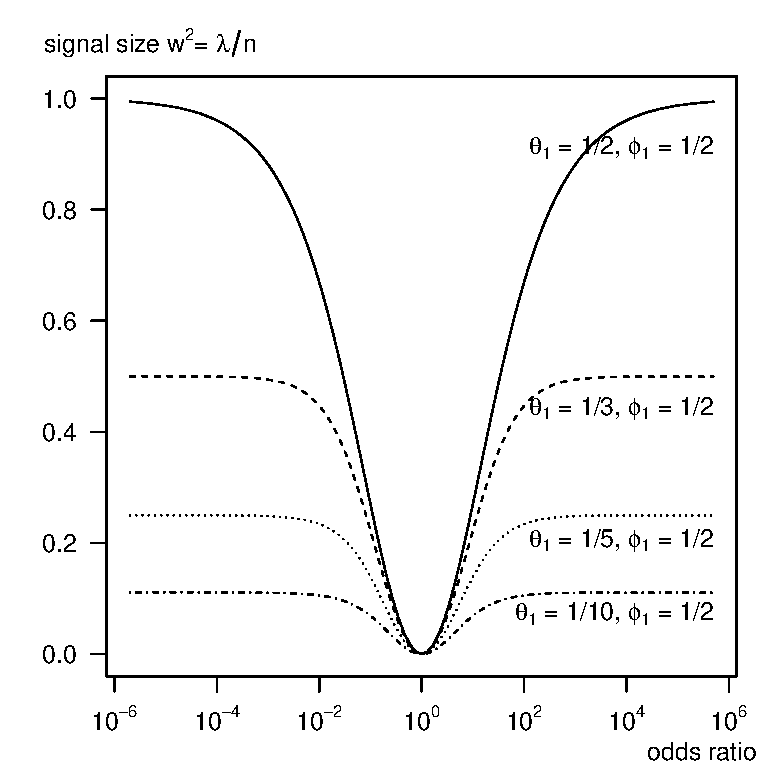
\includegraphics[width=0.49\textwidth]{pics/singal-vs-odds-p05}
      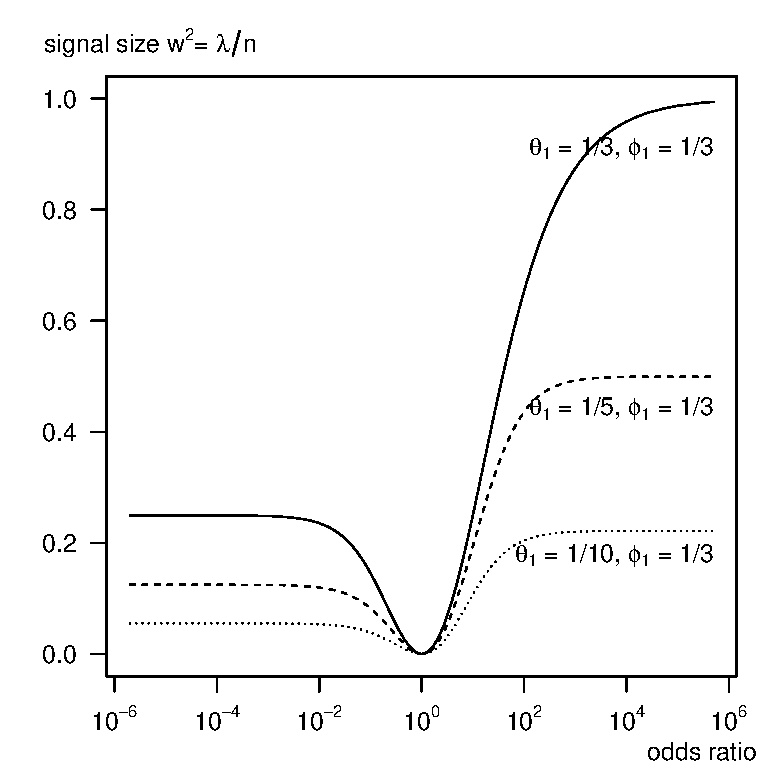
\includegraphics[width=0.49\textwidth]{pics/singal-vs-odds-p0333}            
      \caption{Signal sizes per sample $w^2$ as functions of odds ratios in 2-by-2 multinomial distributions for selected genotype marginals in balanced (left) and unbalanced (right) designs; see Relation \eqref{eq:signal-size-odds-ratio} in Proposition \ref{prop:signal-size-odds-ratio}. For given marginal distributions, extreme odds ratios imply stronger statistical signals at a given sample size. However, the signal sizes are bounded above by constants that depend on the marginal distributions; see Relations \eqref{eq:signal-size-upper-bound-1} and \eqref{eq:signal-size-upper-bound-2}. % Unbalanced marginal distributions -- or rare variants -- lead to smaller signal sizes at a given odds ratio.
      } 
      \label{fig:signal-vs-odds}
\end{figure}

\begin{corollary} \label{cor:signal-limits-OR}
The signal size as a function of the odds ratio $w^2(R)$ is decreasing on $(0,1)$ and increasing on $(1,\infty)$, with limits
\begin{equation} \label{eq:signal-size-upper-bound-1}
    \lim_{\text{R}\to0_+} w^2(\text{R}) = \min\left\{\frac{\phi_1\theta_1}{\phi_2\theta_2}, \frac{\phi_2\theta_2}{\phi_1\theta_1}\right\},
\end{equation}
and
\begin{equation} \label{eq:signal-size-upper-bound-2}
    \lim_{\text{R}\to+\infty} w^2(\text{R}) = \min\left\{\frac{\phi_1\theta_2}{\phi_2\theta_1}, \frac{\phi_2\theta_1}{\phi_1\theta_2}\right\}.
\end{equation}
\end{corollary}
% Proof of Corollary \ref{cor:signal-limits-OR} is found in Appendix \ref{sec:proof-signal-size-odds-ratio}. 

\begin{proof}
	As in the proof of Proposition \ref{prop:signal-size-odds-ratio}, we examine the case where $0<\theta_1,\phi_1\le1/2$, and leave the other three cases an exercise.
	Take the first derivative of the expression for $w^2$ in equation \eqref{eq:signal-size-chisq-delta} with respect to $\delta$, it is evident that $w^2(\delta)$ is decreasing on $[\delta_\mathrm{min},0)$, increasing on $(0,\delta_\mathrm{max}]$, with limits
	$$
	\lim_{d\to \delta_\mathrm{min}} w^2(\delta) = \frac{\phi_1\theta_1}{\phi_2\theta_2},
	\quad
	\text{and}
	\quad
	\lim_{d\to \delta_\mathrm{max}} w^2(\delta) = \min\left\{\frac{\phi_1\theta_2}{\phi_2\theta_1}, \frac{\phi_2\theta_1}{\phi_1\theta_2}\right\}.
	$$
\end{proof}

Corollary \ref{cor:signal-limits-OR} immediately implies that balanced designs with roughly equal number of cases and controls are not necessarily the most informative.

For example, in a study where a third of the recruited subjects carry the genetic variant positively correlated with the trait (i.e., $\theta_1=1/3$), an unbalanced design with $\phi_1=1/3$ would maximize $w^2$ at large odds ratios.
This unbalanced design is much more efficient compared to, say, a balanced design with $\phi_1=1/2$.
In the first case, we have $w^2\to1$ as $R\to\infty$; whereas in the second design, $w^2<1/2$ no matter how large $R$ is.
This difference can also be read by comparing the dashed curve ($\theta_1=1/3$, $\phi_1=1/2$) in the left panel of Figure \ref{fig:signal-vs-odds}, with the solid curve ($\theta_1=1/3$, $\phi_1=1/3$) in the right panel of Figure \ref{fig:signal-vs-odds}.



\section{Optimal study designs and rare variants}
\label{sec:optimal-design} 
For a study with a fixed budget, i.e., a fixed total number of subjects $n$, the researcher is free to choose the fraction of cases $\phi_1$ to be included in the study.
A natural question is how this budget should be allocated to maximize the statistical power of discovery, or equivalently, the signal sizes $\lambda=nw^2$.

In principal, Relation \eqref{eq:signal-size-odds-ratio} can be optimized with respect to the fraction of cases $\phi_1$ in order to find optimal designs, if $\theta_1$ is known and held constant.
In practice, this is not the case.
While the fraction of cases can be controlled, the distributions of genotypes \emph{in the study} are often unknown prior to data collection, and can change with the case-to-control ratio.

Fortunately, the conditional distributions of genotypes in the healthy control groups are often estimated by existing studies, and are made available by consortia such as the NHGRI-EBI GWAS catalog \citep{macarthur2016new}.
% Assume (after appropriate relabelling, hence without loss of generality) that the first variant is associated with an increased risk of disease, and is henceforth referred to as the risk variant.
We denote the conditional frequency of the first genetic variant in the control group as $(f, 1-f)$, where
\begin{equation} \label{eq:RAF}
    f := \mu_{21} / \phi_2.
\end{equation}
The multinomial probability is fully parametrized by the new trio: $(f, \phi_1, R)$.
\begin{center}
    \begin{tabular}{cccc}
    \hline
    & \multicolumn{2}{c}{Genotype} \\
    \cline{2-3}
    Probabilities & Variant 1 & Variant 2 & Total by phenotype \\
    \hline
    Cases & $\frac{\phi_1fR}{fR+1-f}$ & $\frac{\phi_1(1-f)}{fR+1-f}$ & $\phi_1$ \\
    Controls & $f(1-\phi_1)$ & $(1-f)(1-\phi_1)$ & $1-\phi_1$ \\
    \hline
    \end{tabular}
\end{center}
Proposition \ref{prop:signal-size-odds-ratio} may also be re-stated in terms of the new parametrization.

% Note that all these quantities refer to what is in the study, and differ from their counterparts in the general population.

\begin{corollary} \label{cor:signal-size-odds-ratio-conditional-frequency}
In the 2-by-2 multinomial distribution with marginals $(\phi_1, \phi_2 = 1-\phi_1)$, and conditional distribution of the variants in the control group $(f, 1-f)$,
Relation \eqref{eq:signal-size-odds-ratio} holds with $\theta_1 = {\phi_1fR}/{(fR+1-f)} + f(1-\phi_1)$ and $\theta_2 = 1-\theta_1$.
\end{corollary} 

The choice of $\phi_1$ now has a practical solution.

\begin{corollary} \label{cor:optimal-design}
In the context of Corollary \ref{cor:signal-size-odds-ratio-conditional-frequency},
the optimal design $(\phi^*_1, \phi^*_2)$ that maximizes the signal size per sample $w^2$ is prescribed by
\begin{equation} \label{eq:optimal-design}
    \phi_1^* = \frac{fR+1-f}{fR+1-f+\sqrt{R}}, \quad\text{and}\quad 
    \phi_2^* = 1-\phi_1^*.
\end{equation}
% when the denominator in \eqref{eq:optimal-design} is non-zero; otherwise, $\phi_1^*=\phi_2^*=1/2$.
\end{corollary} 


\begin{proof}
	Using the parametrization in \eqref{eq:reparametrize-2-by-2-table-1}, we solve for $\delta$ in \eqref{eq:odds-ratio-delta} to obtain
	\begin{align}
		\delta &= \frac{\phi_1 fR}{fR+1-f} - \left(\frac{\phi_1 fR}{fR+1-f} + f(1-\phi_1)\right)\phi_1 \nonumber \\
		&= \frac{f(1-f)\phi_1(1-\phi_1)(R-1)}{fR+1-f}. \label{eq:reparametrize-2-by-2-table-2}
	\end{align}
	Substituting \eqref{eq:reparametrize-2-by-2-table-2} into the expression \eqref{eq:signal-size-chisq-delta}, after some simplification, yields
	\begin{equation} \label{eq:reparametrize-2-by-2-table-3}
	w^2 = \frac{f(1-f)\phi_1(1-\phi_1)(R-1)^2}{\left[\phi_1 R + (1-\phi_1)D\right]\left[\phi_1 + (1-\phi_1)D\right]},
	\end{equation}
	where $D = fR+1-f > 0$.
	Therefore, he derivative of \eqref{eq:reparametrize-2-by-2-table-3} with respect to $\phi_1$ is
	\begin{equation} \label{eq:signal-size-first-derivative}
	\frac{\mathrm{d}w^2}{\mathrm{d}\phi_1} = 
	\frac{f(1-f)(R-1)^2}{\left[\phi_1 R+(1-\phi_1)D\right]^2 \left[\phi_1+(1-\phi_1)D\right]^2} \left[(D^2-R)\phi_1^2 - 2D^2\phi_1 + D^2\right].
	\end{equation}
	Further, we obtain the second derivative with respect to $\phi_1$,
	\begin{equation} \label{eq:signal-size-second-derivative}
	\frac{\mathrm{d}^2w^2}{\mathrm{d}\phi_1^2} = 
	h(R,f) \left[(\phi_1-1)D^2 - \phi_1R\right],
	\end{equation}
	where $h$ is some function of $(R,f)$ taking on strictly positive values.
	
	Since $\left[(\phi_1-1)D^2 - \phi_1R\right]<0$, the second derivative \eqref{eq:signal-size-second-derivative} must be strictly negative on $[0,1]$.
	This implies that the first derivative \eqref{eq:signal-size-first-derivative} is strictly decreasing on $[0,1]$. 
	Since the first derivative \eqref{eq:signal-size-first-derivative} is strictly positive at $\phi_1=0$, and strictly negative at $\phi_1=1$, it must have a unique zero between 0 and 1, and hence, the solution to $(D^2-R)\phi_1^2 - 2D^2\phi_1 + D^2 = 0$ in the interval of $[0,1]$ must be the maximizer of \eqref{eq:reparametrize-2-by-2-table-3} --- when $D^2-R>0$, the smaller of the two roots maximizes \eqref{eq:reparametrize-2-by-2-table-3}, and when $D^2-R<0$, it is the larger of the two.
	They share the same expression ${D}/{(D+\sqrt{R})}$, which coincides with \eqref{eq:optimal-design}.
	Finally, when $D^2=R$, the only root $\phi_1^*=1/2$, which also coincides with \eqref{eq:optimal-design}, is the maximizer of \eqref{eq:reparametrize-2-by-2-table-3}.
\end{proof}

Of particular interest in the genetics literature are genetic variants with very low allele frequencies in the control group (i.e., $f\approx 0$), known as rare variants.
In such cases, Equation \eqref{eq:optimal-design} can be approximated using the Taylor expansion,
\begin{equation} \label{eq:optimal-design-approx}
    \phi_1^* = \frac{1}{1 + \sqrt{R}} + \frac{(R-\sqrt{R})f}{1+\sqrt{R}} + O(f^2).
\end{equation}
To illustrate, for rare and adversarial factors ($f\approx0$ and $R>1$), the optimal $\phi_1^*$ is less than $1/2$.
Therefore, for studies under a fixed budget, controls should constitute the majority of the subjects, in order to maximize power.
On the other hand, for rare and protective factors ($f\approx0$ and $R<1$), the optimal $\phi_1^*$ is greater than $1/2$, and cases should be the majority.



\section{Phase transitions in large-scale association screening studies}
\label{sec:phase-transitions-in-GWAS}
% Specifically, we develop recipes to find suitable designs of association studies such that combination of the dimensionality $p$, sparsity $\beta$, and signal sizes $r$ of the problem lands in the desired region of risk control, as predicted by the results in Section \ref{sec:chisq-boundaries}.

% Of course, in applications, not all three of the parameters $(p, \beta, r)$ can be altered as we wish.
% In particular, the problem dimensions and sparsity levels are usually determined by the underlying physical processes.
% In the GWAS example, the number of genomic marker locations is determined by the chip used for gene sequencing, while the number of relevant genomic locations is a consequence of the biological process.
% Therefore, in order to achieve a desired level of error control, we can often only hope to influence the statistical signal sizes.

Returning to the problem of \emph{high-dimensional} marginal screenings for categorical covariates, we explore the manifestation of the phase transition in the exact-approximate support recovery problem in the genetic context.

Recall Theorem \ref{thm:chi-squared-exact-approx-boundary} predicts that FWER and FNR can be simultaneously controlled in large dimensions if and only if 
\begin{equation}
    r = \frac{\lambda}{2\log{p}} = \frac{w^2n}{2\log{p}} > 1.
\end{equation}
Therefore, if we were to apply FWER-controlling procedures at low nominal levels (say, $5\%$), then the FNR would experience a phase transition in the sense that, if
\begin{equation} \label{eq:power-1-region}
    r>1 \iff w^2 > \frac{2\log{p}}{n},
\end{equation}
then the FNR can be close to 0; otherwise, FNR must be close to 1.

% Translating this result into the language of association tests, 
Using the parametric relationship described in Corollary \ref{cor:signal-size-odds-ratio-conditional-frequency} (and Proposition \ref{prop:signal-size-odds-ratio}), 
the inequalities in \eqref{eq:power-1-region} implicitly define regions of $(f, R)$ where associations are discoverable with high power, for a given $\phi_1$.
Further, the boundary of such discoverable regions sharpens as dimensionality diverges. 
We illustrate this phase transition through a numerical example next.


\begin{figure}
      \centering
      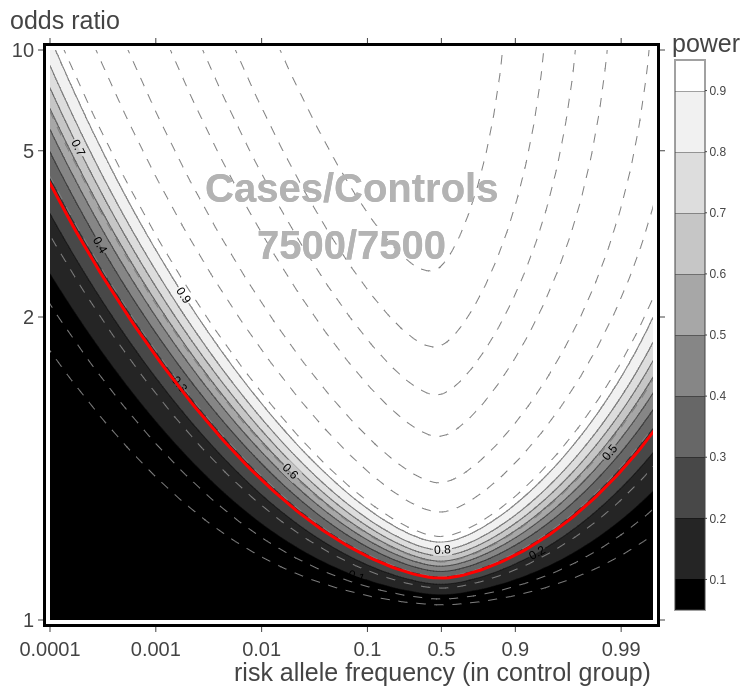
\includegraphics[width=0.49\textwidth]{OR-RAF_plots/OR-RAF_p4.png} 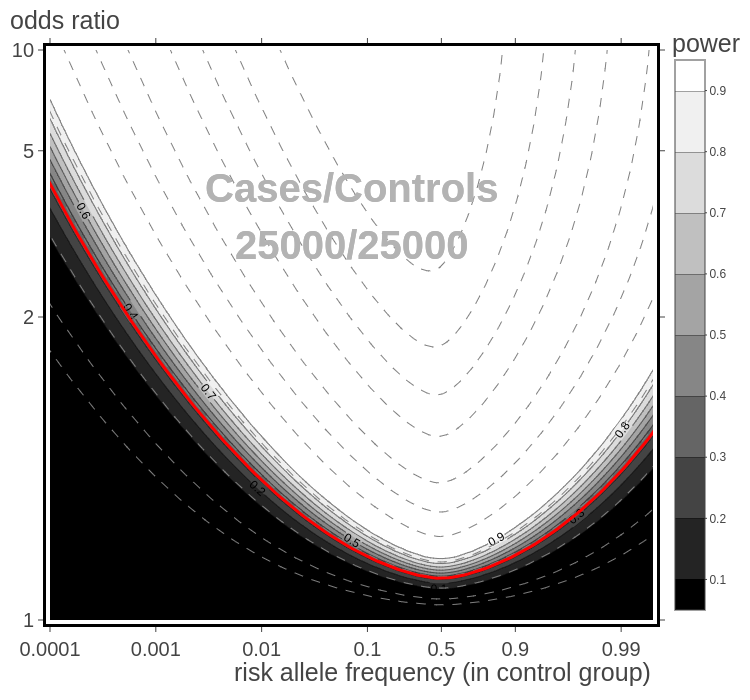
\includegraphics[width=0.49\textwidth]{OR-RAF_plots/OR-RAF_p1e2.png} 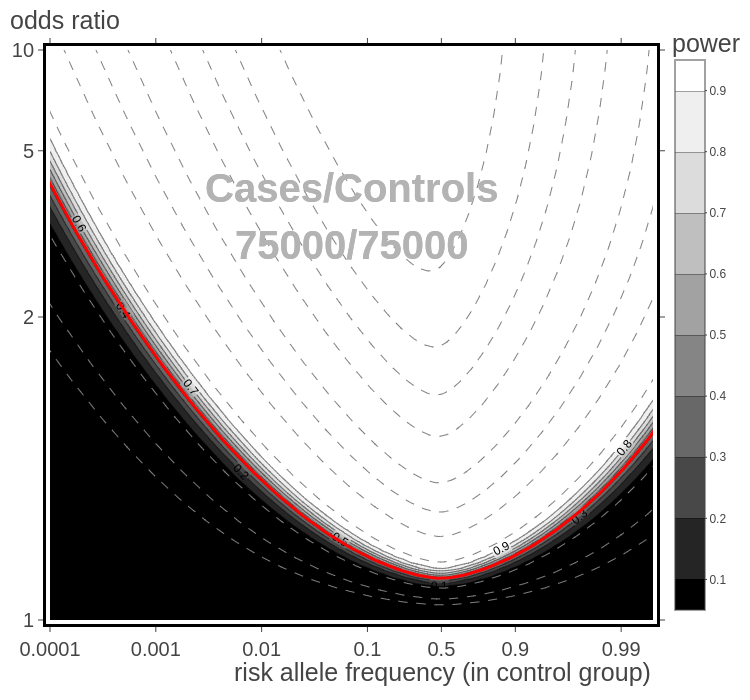
\includegraphics[width=0.49\textwidth]{OR-RAF_plots/OR-RAF_p1e6.png} 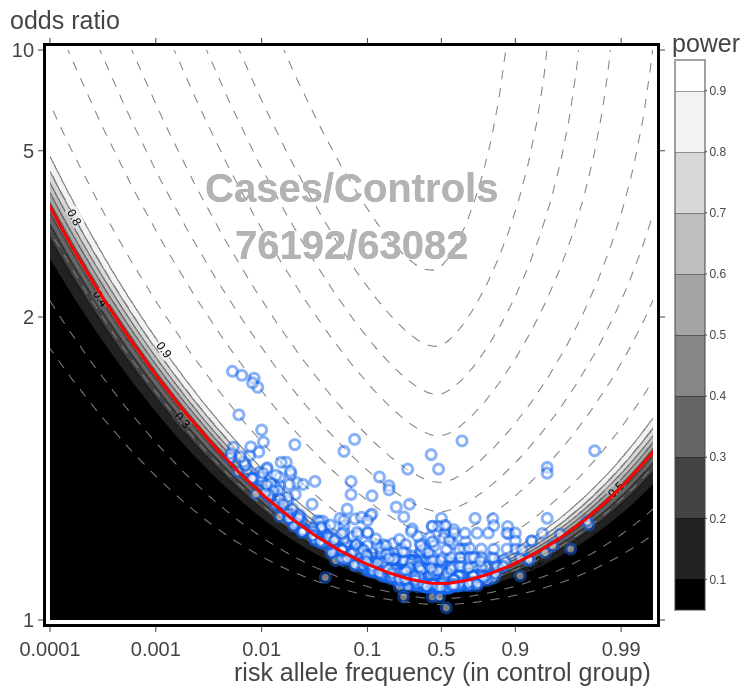
\includegraphics[width=0.49\textwidth]{OR-RAF_plots/OR-RAF_BC_study.png}
      \caption{The OR-RAF diagram visualizing the marginal power of discovery in genetic association studies, after applying Bonferroni's procedure with nominal FWER at $5\%$ level. Sample sizes are marked in each panel, and the problem dimensions are, respectively, $p=4$ (upper-left), $p=10^2$ (upper-right), and $p=10^6$ (lower-left), so that $n/\log{p}$ are roughly constant. Red curves mark the boundaries ($r=1$) of the phase transition for the exact-approximate support recovery problem; dashed curves are the equi-signal (equi-power) curves. The phase transition in signal sizes $\lambda$ translates into the phase transition in terms of $(f,R)$, and sharpens as $p\to\infty$; see Example \ref{exmp:OR-RAF_phase_transition}. In the lower-right panel, we visualize discovered associations (blue circles) in a recent GWA study (Michailidou et al. (2017)); the estimated odds ratios and risk allele frequencies are subject to survival bias and should not be taken at their face values; see Remark \ref{rmk:OR-RAF_false_evidence}.
      } 
      \label{fig:OR-RAF_GWAS}
\end{figure}


\begin{example}
\label{exmp:OR-RAF_phase_transition}
Consider association tests on $2\times2$ contingency tables at $p$ locations as introduced in Section \ref{sec:motivation-chisq}, where the counts follow 
a multinomial distribution
% independent binomial distributions 
% $$
% O_{11} \sim \mathrm{Binom}(n\phi_1, fR/(fR+1-f)),\quad 
% O_{21} \sim \mathrm{Binom}(n(1-\phi_1), fR/(fR+1-f)),
% $$
parametrized by $(f, R, \phi_1)$ as in Section \ref{sec:optimal-design}.
Assume that the phenotype marginals are fixed at $\phi_1 = \phi_2 = 1/2$.
% --- as is the case in genetic association studies --- 
Applying Bonferroni's procedure with nominal FWER at $\alpha=5\%$ level, we can approximate the marginal power of association tests by
\begin{equation} \label{eq:power-approximation}
    \P[\chi^2_{1}(\lambda)>\chi^2_{1,\alpha/p}],
\end{equation}
where $\chi^2_{1,\alpha/p}$ is the upper $(\alpha/p)$-quantile of a central chi-squared distribution with 1 degree of freedom.
We calculate this marginal power as a function of the parameters $(f,R)$ in three scenarios:
\begin{itemize}
    \item $p=4$, $n=3\times10^4$ 
    \item $p=10^2$, $n=1\times10^5$
    \item $p=10^6$, $n=3\times10^6$
\end{itemize}
and visualize the results as heatmaps\footnote{Since genetic variants can always be relabelled such that Variant 1 is positively associated with Cases, we only produce part of the diagram where $R>1$.
Sample sizes marked in the figure are adjusted by a factor of $1/2$, to reflect the genetic context where a pair of alleles are measured for every individual at every genomic location.} (referred to as OR-RAF diagrams) in Figure \ref{fig:OR-RAF_GWAS}.
These parameter values are chosen so that $\log{p}/n$ are roughly constant (around $4.6\times10^{-5}$).

We also overlay ``equi-signal'' curves, i.e., functions implicitly defined by the equations $r=c$ for a range of $c$ (dashed curves), and highlight the predicted boundary of phase transition for the exact-approximate support recovery problem $r=1$ (red curves).
The change in marginal power clearly sharpens around the predicted boundary $r=1$ as dimensionality diverges.
\end{example}

% --- or equivalently, the marginal power ---


\begin{remark}
\label{rmk:OR-RAF_false_evidence}
In an attempt to find empirical evidence of our theoretical predictions, we chart the genetic variants associated with breast cancer, discovered in a 2017 study by \citet{michailidou2017association} in an OR-RAF diagram. 
The estimated risk allele frequencies ($f$) and odds ratios ($R$) are taken from the NHGRI-EBI GWAS catalog \cite{macarthur2016new}, and plotted against a power heatmap calculated according to the reported sample sizes. 
See lower-right panel of Figure \ref{fig:OR-RAF_GWAS}.

It is tempting to believe, on careless inspection, that roughly \emph{all} discovered associations fall inside the high power region of the diagram, therefore demonstrating the phase transition in statistical power.
Unfortunately, the estimates here are subject to survival {bias} --- the study in fact uses the {same} dataset for \emph{both} support estimation and parameter estimation, without adjusting the latter for the selection process.
The seemingly striking agreement between the power calculations and the estimated effects of reported associations \emph{should not} be taken as evidence for the validity of our theory.
We conjecture, as the theory predicts, that accurate and unbiased parameter estimates from an independent replication will still place the associations in the high power region of the diagram. 
\end{remark}

Finally, we demonstrate with an example how results in Sections \ref{sec:chisq-boundaries} and \ref{sec:odds-and-power} may be used for planning prospective association studies.

\begin{example}
In a GWAS with $p = 10^6$ genomic marker locations, researchers wish to locate genetic associations with the trait of interest.
Specifically, they wish to maximize power in the region where genetic variants have risk allele frequencies of $0.01$ and odds ratios of $1.2$.
By Corollary \ref{cor:optimal-design}, the optimal design has a fraction of cases $\phi^* = 0.478$, yielding the statistical signal size per sample $w^2\approx9.00\times10^{-5}$ according to Corollary \ref{cor:signal-size-odds-ratio-conditional-frequency}.

If we wish to achieve exact-approximate support recovery in the sense of \eqref{eq:support-recovery-success}, Theorem \ref{thm:chi-squared-exact-approx-boundary} predicts that the signal size parameter $r$ has to be at least $\widetilde{g}(\beta)= 1$.
This signal size calls for a sample size of $n = \lambda / w^2 = 2r\log(p)/w^2 \approx 307,011$.
In a typically GWAS, a pair of alleles are sequenced for every marker location, bringing the required number of subjects in the study to $n/2 \approx 153,509$.
\end{example}

In comparison, a more accurate power calculation directly using \eqref{eq:power-approximation} predicts that $n / 2 = 165,035$ subjects are needed, under the set of parameters ($p=10^6$, $f=0.01$, $R=1.2$) and $\mathrm{FWER}=0.05$, $\mathrm{FNR}=0.5$; this is $7\%$ higher than our crude asymptotic approximation.
% The accuracy of the asymptotic approximations, by nature of the statements in Theorem \ref{thm:chi-squared-exact-boundary} and \ref{thm:chi-squared-approx-boundary}, depends on how close the error metrics are to zero.
% For example, the number of subjects needed for $\mathrm{FWER}=\mathrm{FWNR}=0.01$ is $499,598$, an $8\%$ increase over the asymptotic prediction; at $\mathrm{FWER}=\mathrm{FWNR}=0.1$, this number becomes $398,996$, some $14\%$ lower than the asymptotic result.
In general, we recommend using the more precise calculations over the back-of-the-envelope asymptotics for planning prospective studies and performing systematic reviews;
a user-friendly web application implementing the more precise approximations is provided in \cite{gao2019upass}.
Nevertheless, the theoretical results on phase transitions generate simple, accurate, and powerful insights that cannot be easily derived from numerical calculations.




\section{Numerical illustrations of the phase transitions in chi-square models}
\label{sec:numerical}
We illustrate with simulations the phase transition phenomena in the chi-square model, and compare numerically the required signal sizes in support recovery problems between the two types of alternatives in the additive error model.
% We also demonstrate the fundamental trade-off between odds ratios and relative frequencies in association studies, as outlined in Proposition \ref{prop:signal-size-odds-ratio} and Corollary \ref{cor:signal-size-odds-ratio-conditional-frequency}, using evidence from large-scale genetic studies.

\subsection{Exact support recovery}

The sparsity of the signal vectors in the experiments are parametrized as in \eqref{eq:signal-sparsity}. 
Signal sizes are assumed equal with magnitude $\lambda(i)=2r\log{p}$ for $i\in S$.
We estimate the support set $S$ using Bonferroni's procedure with nominal FWER level set at $1/(5{\log{p}})$.
The nominal FWER levels vanishes slowly, in line with the assumptions in Theorem \ref{thm:chi-squared-exact-boundary}.
Experiments were repeated 1000 times at each of the 400 sparsity-signal-size combinations, for dimensions $p=10^2, 10^3$, and $10^4$.

The empirical probabilities of exact support recovery under Bonferroni's procedure are shown in Figure \ref{fig:phase-simulated-chi-squared}.
The numerical results suggest not only good accuracy of the predicted boundaries in high-dimensions ($p=10^4$, right panels of Figure \ref{fig:phase-simulated-chi-squared}), but also practical relevance of the theoretical predictions in moderate dimensions ($p=100$, left panels of Figure \ref{fig:phase-simulated-chi-squared}).

\begin{figure}
      \centering
      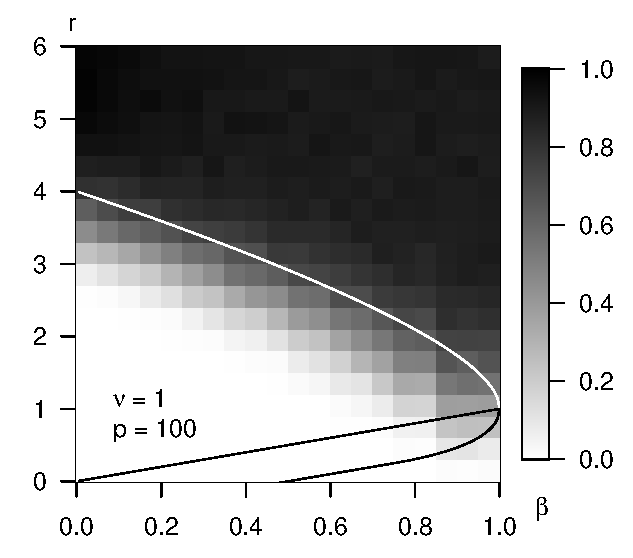
\includegraphics[width=0.32\textwidth]{sim_strong_boundary/simulated_phase_diagram_chi-squared_nu1_p100.eps}
      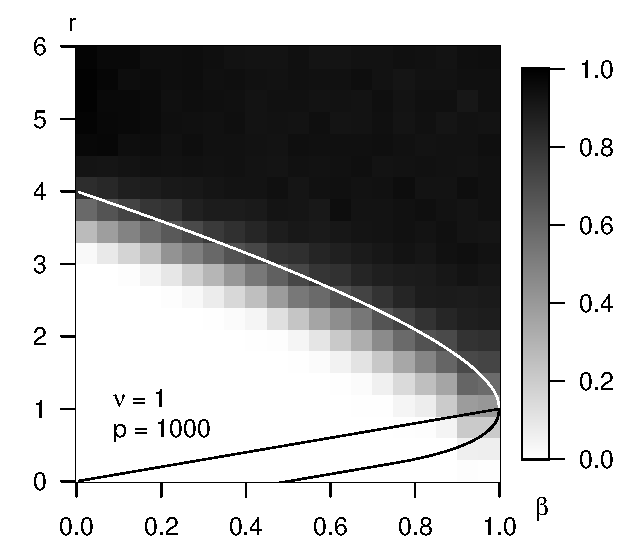
\includegraphics[width=0.32\textwidth]{sim_strong_boundary/simulated_phase_diagram_chi-squared_nu1_p1000.eps}
      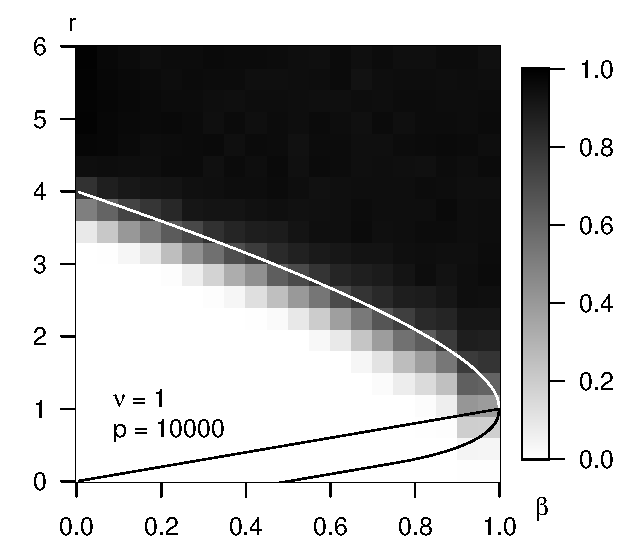
\includegraphics[width=0.32\textwidth]{sim_strong_boundary/simulated_phase_diagram_chi-squared_nu1_p10000.eps}
      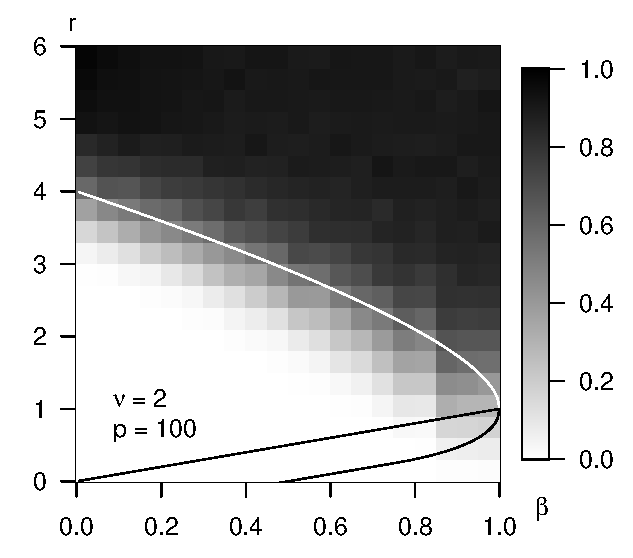
\includegraphics[width=0.32\textwidth]{sim_strong_boundary/simulated_phase_diagram_chi-squared_nu2_p100.eps}
      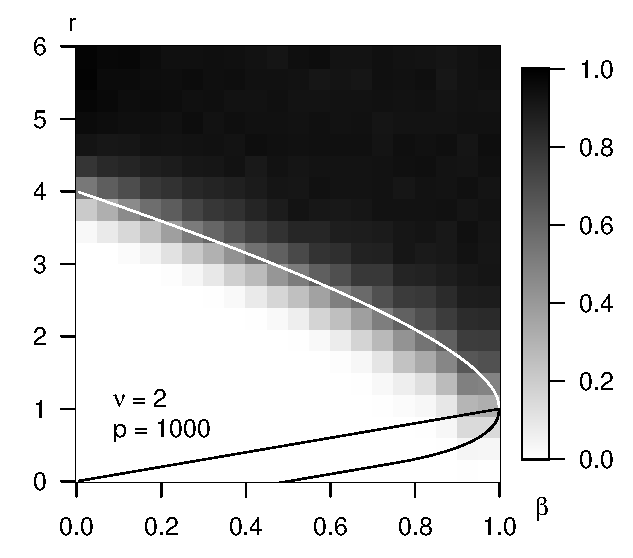
\includegraphics[width=0.32\textwidth]{sim_strong_boundary/simulated_phase_diagram_chi-squared_nu2_p1000.eps}
      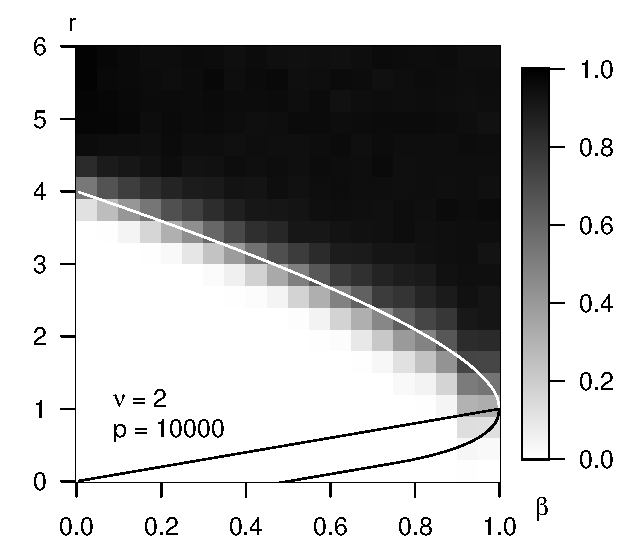
\includegraphics[width=0.32\textwidth]{sim_strong_boundary/simulated_phase_diagram_chi-squared_nu2_p10000.eps}
      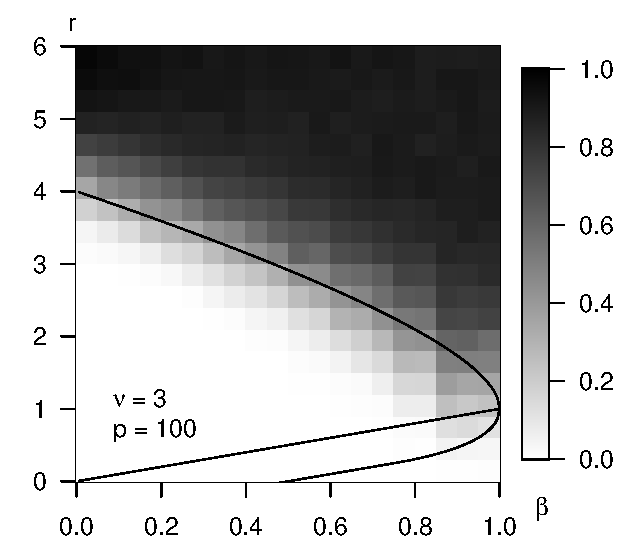
\includegraphics[width=0.32\textwidth]{sim_strong_boundary/simulated_phase_diagram_chi-squared_nu3_p100.eps}
      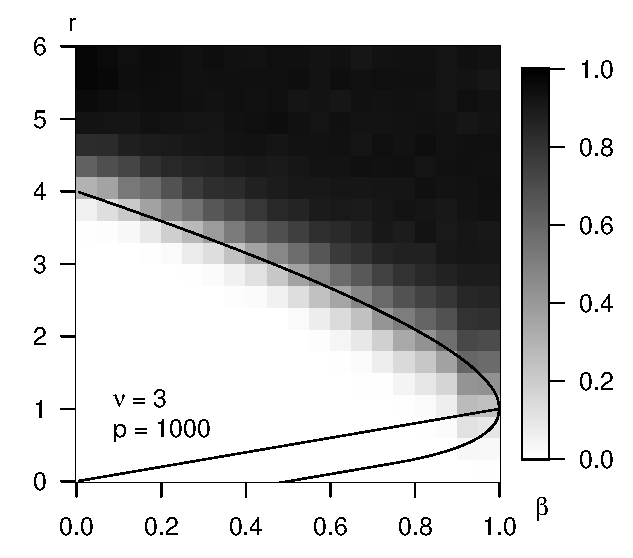
\includegraphics[width=0.32\textwidth]{sim_strong_boundary/simulated_phase_diagram_chi-squared_nu3_p1000.eps}
      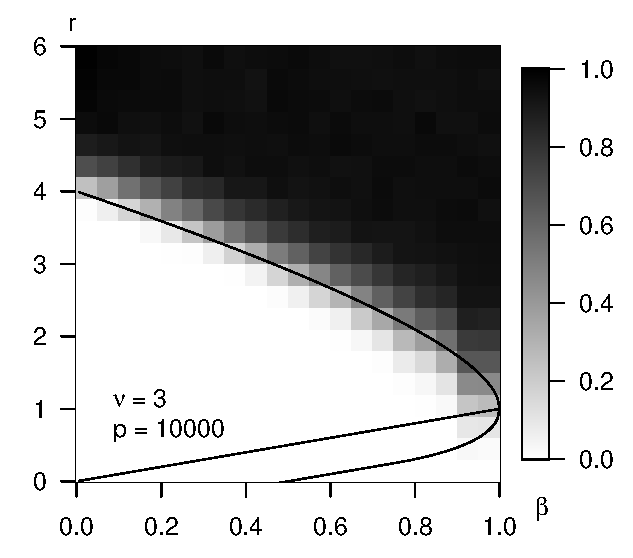
\includegraphics[width=0.32\textwidth]{sim_strong_boundary/simulated_phase_diagram_chi-squared_nu3_p10000.eps}
      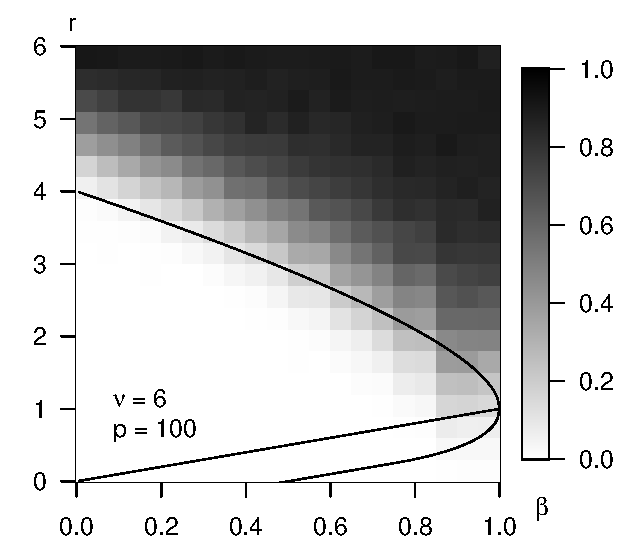
\includegraphics[width=0.32\textwidth]{sim_strong_boundary/simulated_phase_diagram_chi-squared_nu6_p100.eps}
      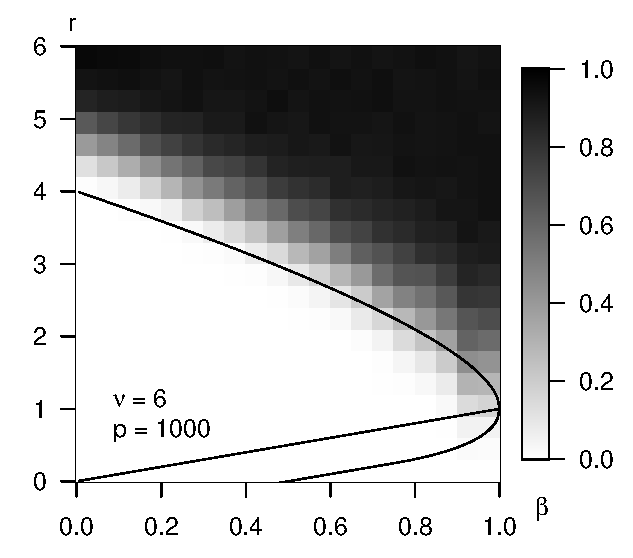
\includegraphics[width=0.32\textwidth]{sim_strong_boundary/simulated_phase_diagram_chi-squared_nu6_p1000.eps}
      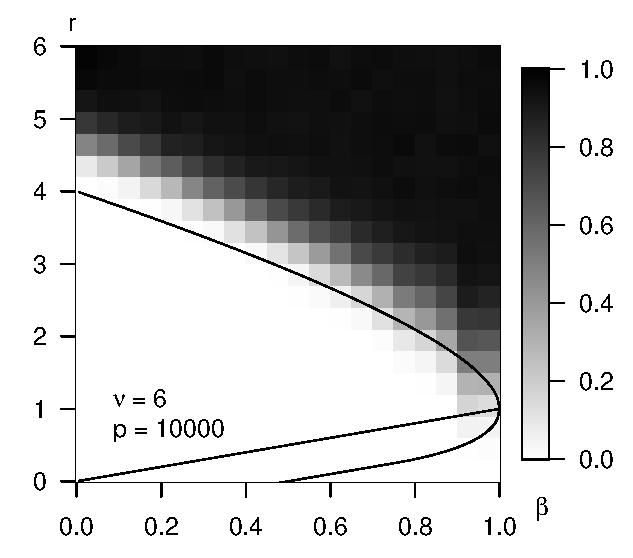
\includegraphics[width=0.32\textwidth]{sim_strong_boundary/simulated_phase_diagram_chi-squared_nu6_p10000.eps}
      \caption{The empirical probability of exact support recovery of Bonferroni's procedure in the chi-squared model \eqref{eq:model-chisq}. 
      We simulate $\nu=1, 2, 3, 6$ (first to last row), at dimensions $p=10^2, 10^3, 10^4$ (left to right column), for a grid of sparsity levels $\beta$ and signal sizes $r$.
      The experiments were repeated 1000 times for each sparsity-signal size combination; darker color indicates higher probability of exact support recovery.  
      Numerical results are in general agreement with the boundaries described in Theorem \ref{thm:chi-squared-exact-boundary}; for large $\nu$'s, the phase transitions take place somewhat above the predicted boundaries.
      The boundary for the approximate support recovery (Theorem \ref{thm:chi-squared-approx-boundary}) and the detection boundary (see Donoho and Jin (2004)) are plotted for comparison.} 
      \label{fig:phase-simulated-chi-squared}
\end{figure}

We conduct further experiments to examine the optimality claims in Theorem \ref{thm:chi-squared-exact-boundary} by comparing with the oracle procedure with thresholds $t_p=\min_{i\in S}x(i)$.
We also examine the claims in Section \ref{subsec:one-vs-two-sided}, and compare the one-sided alternatives in Gaussian additive models with the two-sided alternatives (or equivalently, the chi-square model with $\nu=1$).
We apply Bonferroni's procedure and the oracle thresholding procedure in both settings.

Experiments were repeated 1000 times for a grid of signal size values ranging from $r=0$ to $6$, and for dimensions $10^2, 10^3$, and $10^5$.
Results of the experiments, shown in Figure \ref{fig:one-vs-two-sided-exact_support_recovery}, suggest vanishing difference between difficulties of two-sided vs one-sided alternatives in the additive error models, as well as vanishing difference between the powers of Bonferroni's procedures and the oracle procedures as $p\to\infty$.

\begin{figure}
      \centering
      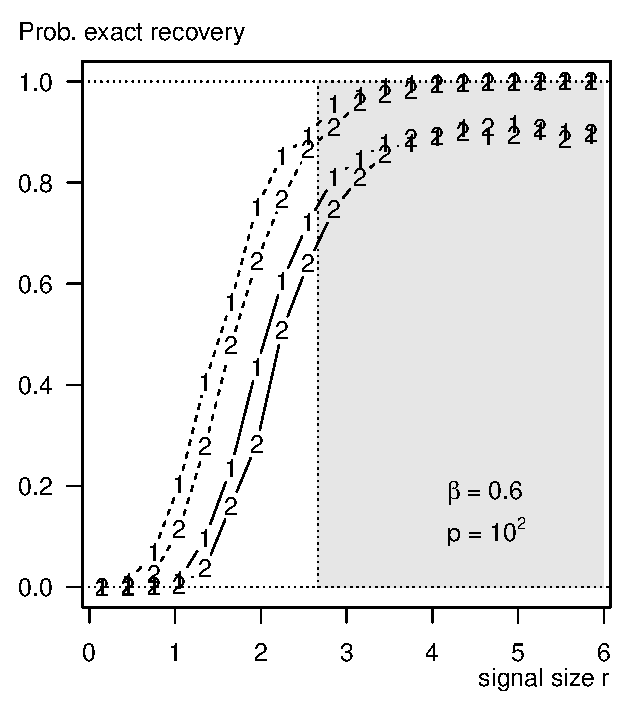
\includegraphics[width=0.32\textwidth]{sim_one-vs-two-sided/exact_recovery_one-vs-two-sided_beta06_p100.eps}
      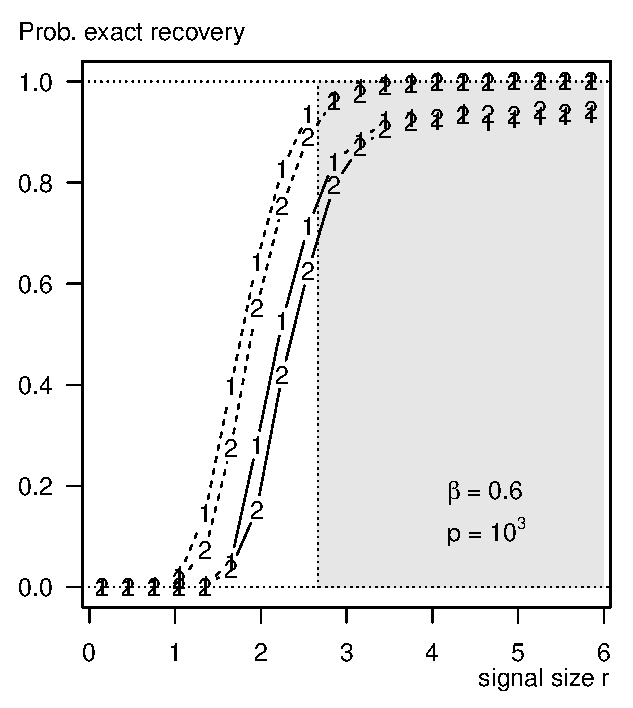
\includegraphics[width=0.32\textwidth]{sim_one-vs-two-sided/exact_recovery_one-vs-two-sided_beta06_p1000.eps}
      % 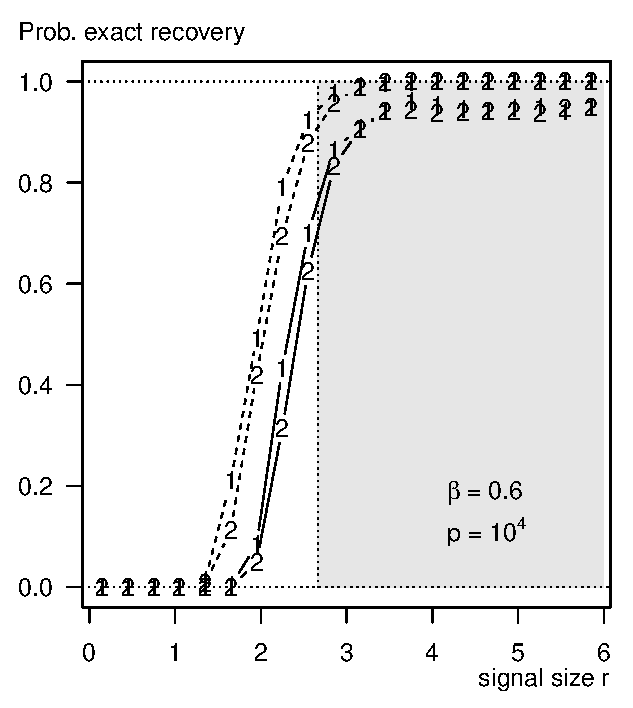
\includegraphics[width=0.33\textwidth]{sim_one-vs-two-sided/exact_recovery_one-vs-two-sided_beta06_p10000.eps}
      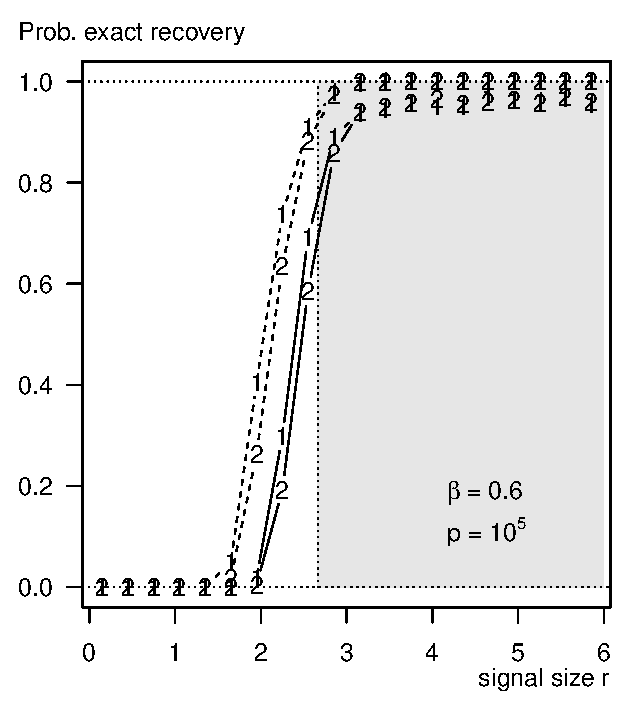
\includegraphics[width=0.32\textwidth]{sim_one-vs-two-sided/exact_recovery_one-vs-two-sided_beta06_p100000.eps}
      \caption{The empirical probability of exact support recovery of Bonferroni's procedure (solid curves) and the oracle procedure (dashed curves) in the chi-squared model with one degree of freedom (marked `2') in the additive Gaussian error model and under one-sided alternatives (marked `1'). 
      We simulate at dimensions $p=10^2, 10^3, 10^5$ (left to right) for a grid of signal sizes $r$ and sparsity level $\beta=0.6$.
      The experiments were repeated 1000 times for each method-model-signal-size combination. 
      Numerical results show evidence of convergence to the 0-1 law as predicted by Theorem \ref{thm:chi-squared-exact-boundary}; regions where asymptotically exact support recovery can be achieved are shaded in grey.
      The difference in power between Bonferroni's procedure and the oracle procedure, as well as in the two types of alternatives both decrease as dimensionality increases.} 
      \label{fig:one-vs-two-sided-exact_support_recovery}
\end{figure}

\subsection{Approximate, and approximate-exact support recovery}

Similar experiments are conducted to examine the optimality claims in Theorem \ref{thm:chi-squared-approx-boundary}, and in Section \ref{subsec:one-vs-two-sided}.
We define an oracle thresholding procedure for approximate support recovery, where the threshold is chosen to minimize the empirical risk.
That is,
$$
t_p(x, S) \in \argmin_{t\in\R} \frac{|\widehat{S}(t)\setminus S|}{\max\{|\widehat{S}(t)|,1\}} + \frac{|S\setminus \widehat{S}(t)|}{\max\{|{S}|,1\}},
%\mathcal{R^\mathrm{oracle}} \in \argmin_{\widehat{S}(\mathcal{R})\in\mathcal{S}} \mathrm{risk}^{\mathrm{A}}(\mathcal{R}),
$$
where $\widehat{S}(t) = \{i\;|\;x(i)\ge t\}$;
in implementation, we only need to scan the values of observations $t\in\{x(1), \ldots, x(p)\}$. 
The nominal FDR level for the BH procedure is set at $1/(5{\log{p}})$, therefore slowly vanishing, in line with the assumptions in Theorem \ref{thm:chi-squared-approx-boundary}; all other parameters are identical to that in the experiments for exact support recovery.
Results of the experiments are shown in Figure \ref{fig:one-vs-two-sided-approx_support_recovery} and Figure \ref{fig:phase-simulated-chi-squared-approx-boundary}.

We also examine the boundary described in Theorem \ref{thm:chi-squared-exact-approx-boundary}.
Experimental settings are identical to that in the experiments for approximate support recovery.
% Results for the BH procedure are in general close to that of the oracle procedure,
We compare the performance of the BH procedure with an oracle procedure with threshold
$$
t_p(x, S) \in \min_{i\in S} x(i),
$$
and visualize results of the experiments in Figure \ref{fig:phase-simulated-chi-squared-approx-exact-boundary}.
Notice that the BH procedure sets its threshold somewhat higher than the oracle, especially for small $\beta$'s. 
The empirical risk of the oracle procedure (not shown here in the interest of space) follows much more closely the predicted boundary \eqref{eq:approx-exact-boundary-chisquared}.

\begin{figure}
      \centering
      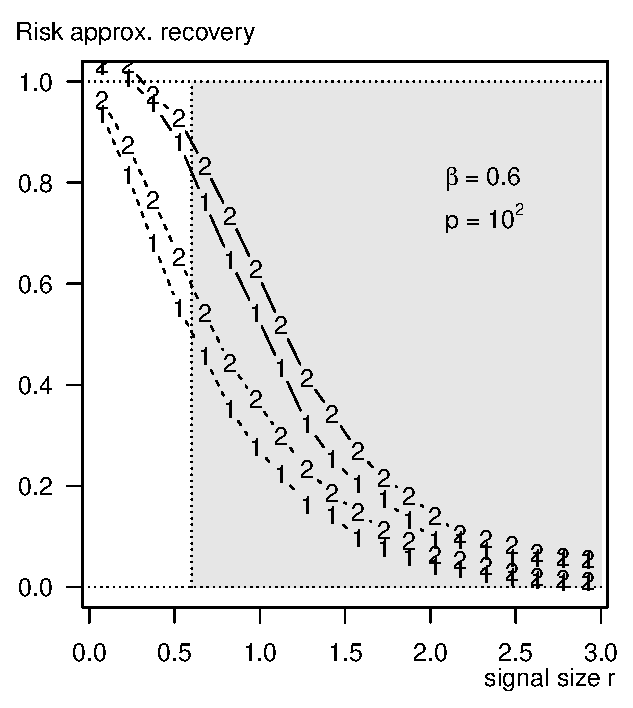
\includegraphics[width=0.32\textwidth]{sim_one-vs-two-sided/approx_recovery_one-vs-two-sided_beta06_p100.eps}
      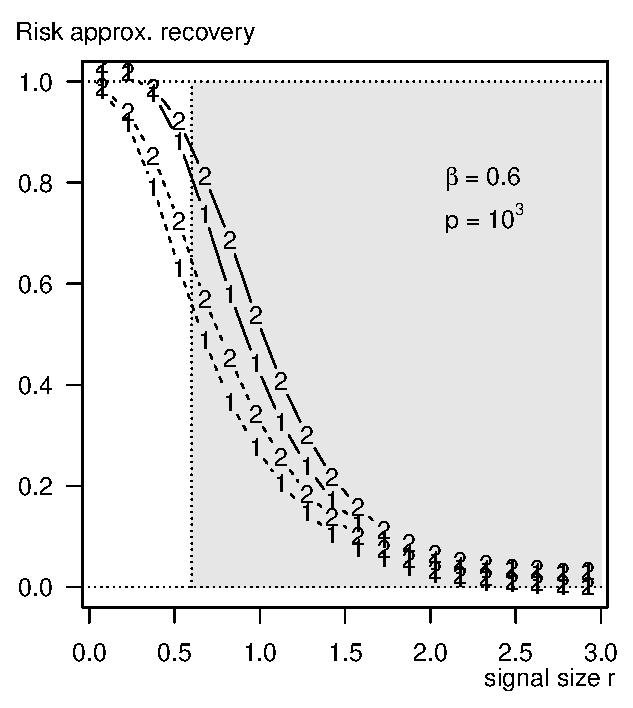
\includegraphics[width=0.32\textwidth]{sim_one-vs-two-sided/approx_recovery_one-vs-two-sided_beta06_p1000.eps}
      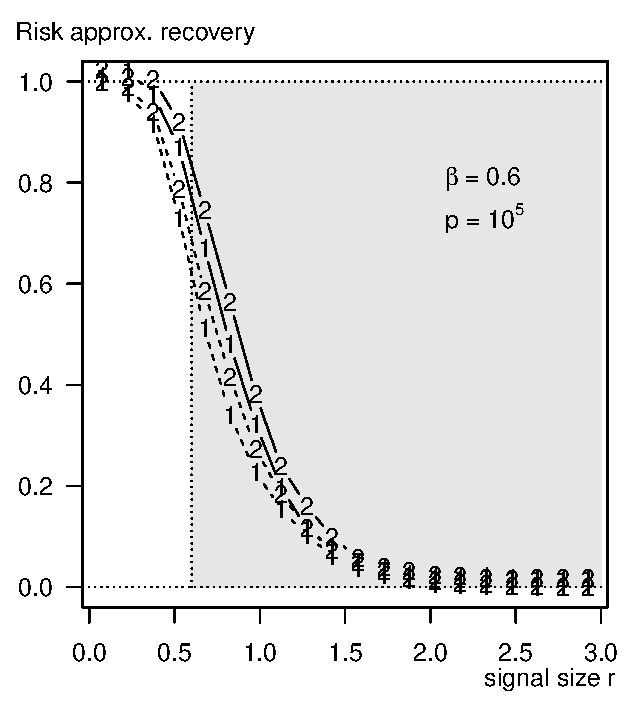
\includegraphics[width=0.32\textwidth]{sim_one-vs-two-sided/approx_recovery_one-vs-two-sided_beta06_p100000.eps}
      \caption{The empirical risk of approximate support recovery of Benjamini-Hochberg's procedure (solid curves) and the oracle procedure (dashed curves) in the chi-squared model with one degree of freedom (marked `2') and in the additive Gaussian error model under one-sided alternatives (marked `1'). 
      We simulate at dimensions $p=10^2, 10^3, 10^5$ (left to right) for a grid of signal sizes $r$ and sparsity level $\beta=0.6$.
      The experiments were repeated 1000 times for each method-model-signal-size combination. 
      Numerical results show evidence of convergence to the 0-1 law as predicted by Theorem \ref{thm:chi-squared-approx-boundary}; regions where asymptotically approximate support recovery can be achieved are shaded in grey.
      The difference in risks between Benjamini-Hochberg's procedure and the oracle procedure, as well as in the two types of alternatives, both decrease as dimensionality increases.} 
      \label{fig:one-vs-two-sided-approx_support_recovery}
\end{figure}


\begin{figure}
      \centering
      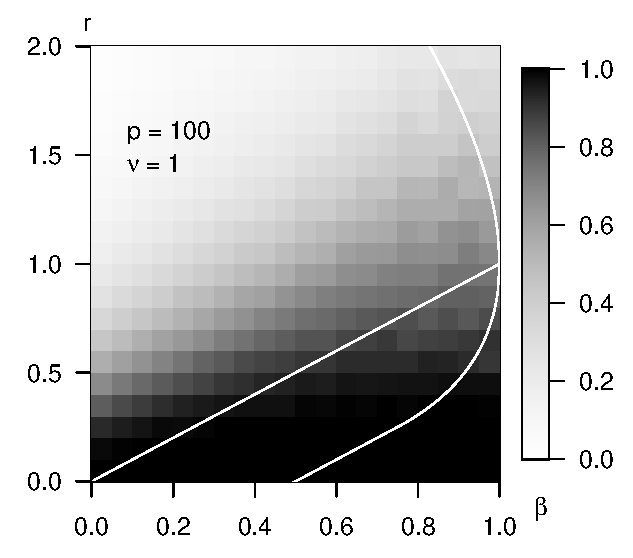
\includegraphics[width=0.32\textwidth]{sim_weak_boundary/simulated_weak_boundary_chi-squared_nu1_p100.eps}
      \includegraphics[width=0.32\textwidth]{sim_weak_boundary/simulated_weak_boundary_chi-squared_nu1_p1000.eps}
      \includegraphics[width=0.32\textwidth]{sim_weak_boundary/simulated_weak_boundary_chi-squared_nu1_p10000.eps}
      \includegraphics[width=0.32\textwidth]{sim_weak_boundary/simulated_weak_boundary_chi-squared_nu2_p100.eps}
      \includegraphics[width=0.32\textwidth]{sim_weak_boundary/simulated_weak_boundary_chi-squared_nu2_p1000.eps}
      \includegraphics[width=0.32\textwidth]{sim_weak_boundary/simulated_weak_boundary_chi-squared_nu2_p10000.eps}
      \includegraphics[width=0.32\textwidth]{sim_weak_boundary/simulated_weak_boundary_chi-squared_nu3_p100.eps}
      \includegraphics[width=0.32\textwidth]{sim_weak_boundary/simulated_weak_boundary_chi-squared_nu3_p1000.eps}
      \includegraphics[width=0.32\textwidth]{sim_weak_boundary/simulated_weak_boundary_chi-squared_nu3_p10000.eps}
      \includegraphics[width=0.32\textwidth]{sim_weak_boundary/simulated_weak_boundary_chi-squared_nu6_p100.eps}
      \includegraphics[width=0.32\textwidth]{sim_weak_boundary/simulated_weak_boundary_chi-squared_nu6_p1000.eps}
      \includegraphics[width=0.32\textwidth]{sim_weak_boundary/simulated_weak_boundary_chi-squared_nu6_p10000.eps}
      \caption{The estimated risk of approximate support recovery $\mathrm{risk}^{\mathrm{A}}$ (see \eqref{eq:risk-approximate}) of the Benjamini-Hochberg procedure in the chi-squared model \eqref{eq:model-chisq}. 
      We simulate $\nu=1, 2, 3, 6$ (first to last row), at dimensions $p=10^2, 10^3, 10^4$ (left to right column), for a grid of sparsity levels $\beta$ and signal sizes $r$.
      The experiments were repeated 1000 times for each sparsity-signal size combination; darker color indicates higher larger $\mathrm{risk}^{\mathrm{A}}$. 
      Numerical results are generally in agreement with the boundaries described in Theorem \ref{thm:chi-squared-approx-boundary}; for large $\nu$'s, the phase transitions take place somewhat above the predicted boundaries.
      The boundary for the exact support recovery problem (Theorem \ref{thm:chi-squared-exact-boundary}) and the detection boundary (see Donoho and Jin (2004)) are plotted for comparison.} 
      \label{fig:phase-simulated-chi-squared-approx-boundary}
\end{figure}


\begin{figure}
      \centering
      \includegraphics[width=0.32\textwidth]{sim_approx-exact_boundary/simulated_approx-exact_boundary_chi-squared_nu1_p100.eps}
      \includegraphics[width=0.32\textwidth]{sim_approx-exact_boundary/simulated_approx-exact_boundary_chi-squared_nu1_p1000.eps}
      \includegraphics[width=0.32\textwidth]{sim_approx-exact_boundary/simulated_approx-exact_boundary_chi-squared_nu1_p10000.eps}
      \includegraphics[width=0.32\textwidth]{sim_approx-exact_boundary/simulated_approx-exact_boundary_chi-squared_nu2_p100.eps}
      \includegraphics[width=0.32\textwidth]{sim_approx-exact_boundary/simulated_approx-exact_boundary_chi-squared_nu2_p1000.eps}
      \includegraphics[width=0.32\textwidth]{sim_approx-exact_boundary/simulated_approx-exact_boundary_chi-squared_nu2_p10000.eps}
      \includegraphics[width=0.32\textwidth]{sim_approx-exact_boundary/simulated_approx-exact_boundary_chi-squared_nu3_p100.eps}
      \includegraphics[width=0.32\textwidth]{sim_approx-exact_boundary/simulated_approx-exact_boundary_chi-squared_nu3_p1000.eps}
      \includegraphics[width=0.32\textwidth]{sim_approx-exact_boundary/simulated_approx-exact_boundary_chi-squared_nu3_p10000.eps}
      \includegraphics[width=0.32\textwidth]{sim_approx-exact_boundary/simulated_approx-exact_boundary_chi-squared_nu6_p100.eps}
      \includegraphics[width=0.32\textwidth]{sim_approx-exact_boundary/simulated_approx-exact_boundary_chi-squared_nu6_p1000.eps}
      \includegraphics[width=0.32\textwidth]{sim_approx-exact_boundary/simulated_approx-exact_boundary_chi-squared_nu6_p10000.eps}
      \caption{The estimated risk of approximate-exact support recovery $\mathrm{risk}^{\mathrm{EA}}$ (see \eqref{eq:risk-approx-exact}) of the Benjamini-Hochberg procedure in the chi-squared model \eqref{eq:model-chisq}. 
      We simulate $\nu=1, 2, 3, 6$ (first to last row), at dimensions $p=10^2, 10^3, 10^4$ (left to right column), for a grid of sparsity levels $\beta$ and signal sizes $r$.
      The experiments were repeated 1000 times for each sparsity-signal size combination; darker color indicates higher larger $\mathrm{risk}^{\mathrm{EA}}$. 
      Numerical results are generally in agreement with the boundaries described in Theorem \ref{thm:chi-squared-approx-exact-boundary}; for small $\beta$'s and large $\nu$'s, the phase transitions take place somewhat above the predicted boundaries.
      Other boundaries in the support recovery and the detection problems are plotted for comparison.} 
      \label{fig:phase-simulated-chi-squared-approx-exact-boundary}
\end{figure}




\section{Proofs}
\label{sec:proof-signal-size-odds-ratio}

We review some properties of the chi-square distributions in Section \ref{sec:chi-square-distributions}, before presenting the proofs of the main theorems on phase transitions in Sections \ref{subsec:proof-chi-squared-exact-boundary}, \ref{subsec:proof-chi-squared-approx-boundary}, and \ref{subsec:proof-chi-squared-mix-boundaries}.
%Results relating signal sizes and effect sizes in association tests will be justified in Section \ref{subsec:proof-signal-size-odds-ratio}.


\section{Auxiliary facts of chi-square distributions}
\label{sec:chi-square-distributions}
We shall recall, and establish, some auxiliary facts about chi-square distributions. 
These facts will be used in the proofs of Theorem \ref{thm:chi-squared-exact-boundary} and Theorem \ref{thm:chi-squared-approx-boundary}.

\begin{lemma}[Rapid variation of chi-square distribution tails] \label{lemma:rapid-variation-chisq}
The central chi-square distribution with $\nu$ degrees of freedom has rapidly varying tails.
That is, 
\begin{equation} \label{eq:rapid-variation-chisq}
    \lim_{x\to\infty}\frac{\P[\chi_\nu^2(0)>tx]}{\P[\chi_\nu^2(0)>x]} = 
    \begin{cases}
    0, & t > 1 \\
    1, & t = 1 \\
    \infty, & 0 < t < 1
\end{cases},
\end{equation}
where we overloaded the notation $\chi_\nu^2(0)$ to represent a random variable with the chi-square distribution.
\end{lemma}

\begin{proof}[Proof of Lemma \ref{lemma:rapid-variation-chisq}]
When $\nu=1$, the chi-square distribution reduces to a squared Normal, and \eqref{eq:rapid-variation-chisq} follows from the rapid variation of the standard Normal distribution.
For $\nu\ge2$, we recall the following bound on tail probabilities (see, e.g., \citep{inglot2010inequalities}),
$$
\frac{1}{2}\mathcal{E}_\nu(x) \le \P[\chi_\nu^2(0)>x] \le \frac{x}{(x-\nu+2)\sqrt{\pi}} \mathcal{E}_\nu(x), \quad \nu\ge2,\;x>\nu-2,
$$
where $\mathcal{E}_\nu(x) = \exp\left\{-\frac{1}{2}[(x-\nu-(\nu-2)\log(x/\nu) + \log\nu]\right\}$.
Therefore, we have 
$$
\frac{(x-\nu+2)\sqrt{\pi}}{2x}\frac{\mathcal{E}_\nu(tx)}{\mathcal{E}_\nu(x)} 
\le \frac{\P[\chi_\nu^2(0)>tx]}{\P[\chi_\nu^2(0)>x]}
\le \frac{2tx}{(tx-\nu+2)\sqrt{\pi}}\frac{\mathcal{E}_\nu(tx)}{\mathcal{E}_\nu(x)},
$$
where ${\mathcal{E}_\nu(tx)}/{\mathcal{E}_\nu(x)} = \exp\{-\frac{1}{2}[(t-1)x-(\nu-2)\log{t}]\}$ converges to $0$ or $\infty$ depending on whether $t>1$ or $0<t<1$.
The case where $t=1$ is trivial.
\end{proof}

Lemma \ref{lemma:rapid-variation-chisq} and Proposition \ref{prop:rapid-varying-tails} yield the following Corollary.

\begin{corollary} \label{cor:relative-stability}
Maxima of independent observations from central chi-square distributions with $\nu$ degrees of freedom are relatively stable. 
Specifically, let $\epsilon_p = \left(\epsilon_p(i)\right)_{i=1}^p$ be independently and identically distributed (iid) $\chi_\nu^2(0)$ random variables. 
Then the triangular array ${\cal E} = \{\epsilon_p, p\in\N\}$ has relatively stable (RS) maxima in the sense of \eqref{eq:RS-condition}.
\end{corollary}


\begin{lemma}[Stochastic monotonicity] \label{lemma:stochastic-monotonicity}
The non-central chi-square distribution is stochastically monotone in its non-centrality parameter.
Specifically, for two non-central chi-square distributions both with $\nu$ degrees of freedom, and non-centrality parameters $\lambda_1 \le \lambda_2$, we have $\chi^2_\nu(\lambda_1) \stackrel{\mathrm{d}}{\le} \chi^2_\nu(\lambda_2)$. 
That is,
\begin{equation} \label{eq:stochastic-monotonicity}
    \P[\chi^2_\nu(\lambda_1) \le t] \ge \P[\chi^2_\nu(\lambda_2) \le t], \quad \text{for any}\quad t\ge0.
\end{equation}
where we overloaded the notation $\chi_\nu^2(\lambda)$ to represent a random variable with the chi-square distribution with non-centrality parameter $\lambda$ and degree-of-freedom parameter $\nu$.
\end{lemma}

\begin{proof}[Proof of Lemma \ref{lemma:stochastic-monotonicity}]
Recall that non-central chi-square distributions can be written as sums of $\nu-1$ standard normal random variables and a non-central normal random variable with mean $\sqrt{\lambda}$ and variance 1,
\begin{equation*}
    \chi_\nu^2(\lambda) 
    \stackrel{\mathrm{d}}{=} Z_1^2 + \ldots + Z_{\nu-1}^2 + (Z_\nu + \sqrt{\lambda})^2.
\end{equation*}
Therefore, it suffices to show that $\P[(Z+\sqrt{\lambda})^2 \le t]$ is non-increasing in $\lambda$ for any $t\ge0$, where $Z$ is a standard normal random variable.
We rewrite this expression in terms of standard normal probability function $\Phi$,
\begin{align}
    \P[(Z+\sqrt{\lambda})^2 \le t] 
    &= \P[-\sqrt{\lambda} - \sqrt{t} \le Z \le -\sqrt{\lambda} + \sqrt{t}] \nonumber \\
    &= \Phi(-\sqrt{\lambda} + \sqrt{t}) - \Phi(-\sqrt{\lambda} - \sqrt{t}). \label{eq:stochastic-monotonicity-proof-1}
\end{align}
The derivative of the last expression (with respect to $\lambda$) is 
\begin{equation} \label{eq:stochastic-monotonicity-proof-2}
    \frac{1}{2\sqrt{\lambda}} \left(\phi(\sqrt{\lambda} + \sqrt{t}) - \phi(\sqrt{\lambda} - \sqrt{t})\right) 
    = \frac{1}{2\sqrt{\lambda}} \left(\phi(\sqrt{\lambda} + \sqrt{t}) - \phi(\sqrt{t} - \sqrt{\lambda})\right),
\end{equation}
where $\phi$ is the density of the standard normal distribution.
Notice that we have used the symmetry of $\phi$ around 0 in the last expression.

Since $0 \le \max\{\sqrt{\lambda} - \sqrt{t}, \sqrt{t} - \sqrt{\lambda}\} < \sqrt{t} + \sqrt{\lambda}$ when $t>0$, by monotonicity of the normal density on $(0,\infty)$, we conclude that the derivative \eqref{eq:stochastic-monotonicity-proof-2} is indeed negative.
Therefore, \eqref{eq:stochastic-monotonicity-proof-1} is decreasing in $\lambda$, and \eqref{eq:stochastic-monotonicity} follows for $t>0$.
For $t = 0$, equality holds in \eqref{eq:stochastic-monotonicity} with both probabilities being 0.
\end{proof}


Finally, we derive asymptotic expressions for  chi-square quantiles.

\begin{lemma}[Chi-square quantiles] \label{lemma:chisq-quantiles}
Let $F$ be the central chi-square distributions with $\nu$ degrees of freedom, and let $u(y)$ be the $(1-y)$-th generalized quantile of $F$, i.e.,
\begin{equation} \label{eq:quantiles-generic}
    u(y) = F^\leftarrow(1 - y).
\end{equation}
Then 
\begin{equation}
    u(y) \sim 2\log(1/y), \quad \text{as }y\to0. 
\end{equation}
\end{lemma}

\begin{proof}[Proof of Lemma \ref{lemma:chisq-quantiles}]
The case where $\nu=1$ follows from the well-known formula for Normal quantiles (see, e.g., Proposition 1.1 in \cite{gao2018fundamental})
$$
F^\leftarrow(1 - y) = \Phi^\leftarrow(1-y/2)\sim\sqrt{2\log{(2/y)}}\sim\sqrt{2\log{(1/y)}}.
$$
The case where $\nu\ge2$ follows from the following estimates of high quantiles of chi-square distributions (see, e.g., \citep{inglot2010inequalities}),
$$
    \nu +  2\log(1/y) -5/2 \le u(y) \le \nu +  2\log(1/y) + 2\sqrt{\nu\log(1/y)}, \quad \text{for all }y\le0.17,
$$
where both the lower and upper bound are asymptotic to $2\log(1/y)$.
\end{proof}




\section{Proof of Theorem \ref{thm:chi-squared-exact-boundary}}
\label{subsec:proof-chi-squared-exact-boundary}

\begin{proof}[Theorem \ref{thm:chi-squared-exact-boundary}]
We first prove the sufficient condition.
The Bonferroni procedure sets the threshold at $t_p = F^\leftarrow(1-\alpha/p)$, which, by Lemma \ref{lemma:chisq-quantiles}, is asymptotic to $2\log{p} - 2\log{\alpha}$.
By the assumption on $\alpha$ in \eqref{eq:slowly-vanishing-error}, for any $\delta>0$, we have $p^{-\delta}=o(\alpha)$.
Therefore, we have $-\log\alpha\le\delta\log{p}$ for large $p$, and
\begin{equation*} 
    1 \le \limsup_{p\to\infty}\frac{2\log{p} - 2\log{\alpha}}{2\log{p}} \le 1+\delta,
\end{equation*}
for any $\delta>0$.
Hence, $t_p\sim 2\log{p}$.

The condition $\underline{r} > {{g}}(\beta)$ implies, after some algebraic manipulation,
$\sqrt{\underline{r}} -\sqrt{1-\beta} > 1$.
Therefore, we can pick $q>1$ such that 
\begin{equation} \label{eq:choice-of-q}
    \sqrt{\underline{r}} -\sqrt{1-\beta} > \sqrt{q} > 1.
\end{equation}
Setting the $t^* = t^*_p = 2q\log{p}$, we have $t_p < t^*_p$ for large $p$.

On the one hand, $\text{FWER} = 1 - \P[\widehat{S}_p \subseteq S_p]$ vanishes under the Bonferroni procedure with $\alpha\to0$.
On the other hand, for large $p$, the probability of no missed detection is bounded from below by
\begin{equation} \label{eq:chi-square-sufficient-1}
    \P[\widehat{S}_p \supseteq S_p] 
    = \P[\min_{i\in S} x(i) \ge t_p] 
    \ge \P[\min_{i\in S} x(i) \ge t^*] 
    \ge 1 - p^{1-\beta}\P[\chi_\nu^2(\underline{\Delta}) < t^*],
\end{equation}
where we have used the fact that signal sizes are bounded below by $\underline{\Delta}$, and the stochastic monotonicity of chi-square distributions (Lemma \ref{lemma:stochastic-monotonicity}) in the last inequality.
Writing
$$
\chi_\nu^2(\underline{\Delta}) \stackrel{\mathrm{d}}{=} Z_1^2 + \ldots + Z_{\nu-1}^2 + (Z_\nu + \sqrt{\underline{\Delta}})^2
$$
where $Z_i$'s are iid standard normal variables, we have
\begin{align}
    \P[\chi_\nu^2({\underline{\Delta}}) < t^*]
    &\le \P[(Z_\nu+\sqrt{\underline{\Delta}})^2 < t^*] 
    = \P[|Z_\nu+\sqrt{\underline{\Delta}}| < \sqrt{t^*}]  \nonumber \\
    &\le \P\left[Z_\nu < - \sqrt{\underline{\Delta}} +  \sqrt{t^*}\right] \nonumber \\
    &= \P\left[Z_\nu < \sqrt{2\log{p}}\left(\sqrt{q} - \sqrt{\underline{r}}\right)\right]. \label{eq:chi-square-sufficient-2}
\end{align}
By our choice of $q$ in \eqref{eq:choice-of-q}, the last probability in \eqref{eq:chi-square-sufficient-2} can be bounded from above by 
\begin{align*}
    \P\Big[Z_\nu < -\sqrt{2(1-\beta)\log{p}}\Big]
    &\sim \frac{\phi\left(-\sqrt{2(1-\beta)\log{p}}\right)}{\sqrt{2(1-\beta)\log{p}}} \\
    &= \frac{1}{\sqrt{2(1-\beta)\log{p}}}p^{-(1-\beta)},
\end{align*}
where the first line uses Mill's ratio for Gaussian distributions (see Section \ref{sec:Gaussian} and Relation \eqref{eq:Mills-ratio}).
This, combined with \eqref{eq:chi-square-sufficient-1}, completes the proof of the sufficient condition for the Bonferroni's procedure.

Under the assumption of independence, Sid\'ak's, Holm's, and Hochberg's procedures are strictly more powerful than Bonferroni's procedure, while controlling FWER at the nominal levels.
Therefore, the risks of exact support recovery for these procedures also vanishes.
This completes the proof for the first part of Theorem \ref{thm:chi-squared-exact-boundary}.

We now show the necessary condition. 
We first normalize the maxima by the chi-square quantiles $u_p = F^{\leftarrow}(1-1/p)$, where $F$ is the distribution of a (central) chi-square random variable,
\begin{equation} \label{eq:chi-square-necessary-0}
 \P[\widehat{S}_p = S_p] \le \P\left[M_{S^c} <  t_p \le m_{S} \right]
  % &= \P\left[\frac{\max_{i\in S^c}x(i)}{u_p} < \frac{\min_{i\in S}x(i)}{u_p}\right] \nonumber \\
  % &\le  \P\left[\frac{\max_{i\in S^c}\chi_\nu^2(\lambda(i))}{u_p} < \frac{\min_{i\in S}\chi_\nu^2(\lambda(i))}{u_p}\right] \nonumber \\
  \le \P\left[ \frac{M_{S^c}}{u_p} < \frac{m_S}{u_p} \right],
\end{equation}
where $M_{S^c} = \max_{i\in S^c}x(i)$ and $m_{S} = \min_{i\in S}x(i)$.
By the relative stability of chi-square random variables (Corollary \ref{cor:relative-stability}), we know that ${M_{S^c}}/{u_{|S^c|}}\to1$ in probability. 
Further, using the expression for $u_p$ (Lemma \ref{lemma:chisq-quantiles}), we obtain
$$
\frac{u_{p-p^{1-\beta}}}{u_{p}} \sim \frac{2\log{(p-p^{1-\beta})}}{2\log{p}} = \frac{\log{p}+\log{(1-p^{-\beta})}}{\log{p}} \sim 1.
$$
Therefore, the left-hand-side of the last probability in \eqref{eq:chi-square-necessary-0} converges to 1,
\begin{equation} \label{eq:chi-square-necessary-1}
    \frac{M_{S^c}}{u_{p}} = \frac{M_{S^c}}{u_{p-p^{1-\beta}}} \frac{u_{p-p^{1-\beta}}}{u_{p}} \stackrel{\P}{\longrightarrow} 1.
\end{equation}

Meanwhile, for any $i\in S$, by Lemma \ref{lemma:stochastic-monotonicity} and the fact that signal sizes are bounded above by $\overline{\Delta}$, we have,
\begin{equation*}
    {\chi_\nu^2(\lambda(i))} \stackrel{\mathrm{d}}{\le}
    {\chi_\nu^2(\overline{\Delta})} \stackrel{\mathrm{d}}{=} 
    {Z_1^2 + \ldots + Z_{\nu-1}^2 + \left(Z_\nu + \sqrt{\overline{\Delta}}\right)^2}.
\end{equation*}
Dividing through by $u_p$, and taking minimum over $S$, we obtain
\begin{equation} \label{eq:chi-square-necessary-3}
    \frac{m_S}{u_p} 
    = \min_{i\in S} \frac{\chi_\nu^2(\lambda(i))}{u_p} 
    % \stackrel{\mathrm{d}}{\le} \min \left\{\frac{\chi_\nu^2(\overline{\Delta})}{u_p}, s \text{ iid copies} \right\} \\
    \stackrel{\mathrm{d}}{\le} 
    \min_{i\in S}\left\{\frac{Z_1^2(i) + \ldots + Z_{\nu-1}^2(i)}{u_p} + \frac{(Z_\nu(i) + \sqrt{\overline{\Delta}})^2}{u_p}\right\}.
\end{equation}
Let $i^\dagger = i^\dagger_p$ be the index minimizing the second term in \eqref{eq:chi-square-necessary-3}, i.e.,
\begin{equation}
    i^\dagger := \argmin_{i\in S} \frac{(Z_\nu(i) + \sqrt{\overline{\Delta}})^2}{u_p}
    = \argmin_{i\in S} f_p\left(Z_\nu(i)\right),
    % \frac{(Z_\nu(i) + \sqrt{\overline{\Delta}})^2}{2\log{p}},
\end{equation}
where $f_p(x):=(x+\sqrt{\overline{\Delta}})^2/(2\log{p})$. 
We shall first show that 
\begin{equation} \label{eq:chi-square-necessary-4}
    %\min_{i\in S} \frac{(Z_\nu(i) + \sqrt{\overline{\Delta}})^2}{2\log{p}} 
    \P[ f_p(Z_\nu(i^\dagger)) < 1 -\delta ] \to 1,
\end{equation}
for some small $\delta>0$.
On the one hand, we know (by solving a quadratic inequality) that
\begin{equation} \label{eq:chi-square-necessary-5}
    f_p(x)<1-\delta \iff \frac{x}{\sqrt{2\log{p}}} \in (-(\sqrt{\overline{r}}+\sqrt{1-\delta}), -(\sqrt{\overline{r}}-\sqrt{1-\delta})).
\end{equation}
On the other hand, we know (by the relative stability of iid Gaussians, recall Section \ref{sec:Gaussian}) that 
\begin{equation} \label{eq:chi-square-necessary-6}
    % f_p(\min_{i\in S}z_\nu(i)) =
    \frac{\min_{i\in S} Z_\nu(i)}{\sqrt{2\log{p}}}
    \to -\sqrt{1-\beta} \quad\text{in probability}.
\end{equation}
Further, by the assumption on the signal sizes $\overline{r} < (1+\sqrt{1-\beta})^2$, we have,
\begin{equation*}
    -(\sqrt{\overline{r}}+1) < -1 <- \sqrt{1-\beta} < - (\sqrt{\overline{r}}-1).
\end{equation*}
Therefore we can picking a small $\delta>0$ such that 
\begin{equation} \label{eq:chi-square-necessary-7}
    -(\sqrt{\overline{r}}+1) < -(\sqrt{\overline{r}}+\sqrt{1-\delta})
    < - \sqrt{1-\beta}
    < - (\sqrt{\overline{r}}-\sqrt{1-\delta})
    < - (\sqrt{\overline{r}}-1).
\end{equation}
Combining \eqref{eq:chi-square-necessary-5}, \eqref{eq:chi-square-necessary-6}, and \eqref{eq:chi-square-necessary-7}, we obtain
\begin{align*}
    \P\left[\min_{i\in S} f_p(Z_\nu(i)) < 1-\delta\right]
    &= \P\left[ f_p(Z_\nu(i^\dagger)) < 1-\delta \right] \\
    &\ge \P\left[ f_p\left(\min_{i\in S}Z_\nu(i)\right) < 1-\delta \right] \to 1,
\end{align*}
and we arrive at \eqref{eq:chi-square-necessary-4}.
As a corollary, since $u_p\sim2\log{p}$, it follows that
\begin{equation} \label{eq:chi-square-necessary-8}
    \P\left[\min_{i\in S}\frac{(Z_\nu(i) + \sqrt{\overline{\Delta}})^2}{u_p} < 1-\delta\right]\to1.
\end{equation}

Finally, by independence between $Z_1^2(i)+\ldots+Z_{\nu-1}^2(i)$ and $(Z_\nu^2(i)+\sqrt{\overline{\Delta}})^2$, and the fact that $i^\dagger$ is a function of only the latter, we have
$$
Z_1^2(i^\dagger)+\ldots+Z_{\nu-1}^2(i^\dagger) 
\stackrel{\mathrm{d}}{=} Z_1^2(i)+\ldots+Z_{\nu-1}^2(i) 
\quad \text{for all} \;\; i\in S.
$$
Therefore, $Z_1^2(i^\dagger)+\ldots+Z_{\nu-1}^2(i^\dagger) = O_\P(1)$, and 
\begin{equation} \label{eq:chi-square-necessary-9}
    \frac{Z_1^2(i^\dagger)+\ldots+Z_{\nu-1}^2(i^\dagger)}{u_p} \to 0 \quad \text{in probability}. 
\end{equation}
Together, \eqref{eq:chi-square-necessary-8} and \eqref{eq:chi-square-necessary-9} imply that
\begin{align}
    \P\left[\frac{m_S}{u_p}<1-\delta\right]
    &\ge \P\left[\min_{i\in S}\left\{\frac{Z_1^2(i) + \ldots + Z_{\nu-1}^2(i)}{u_p} + \frac{(Z_\nu(i) + \sqrt{\overline{\Delta}})^2}{u_p}\right\} < 1-\delta\right] \nonumber \\
    &\ge \P\left[\frac{Z_1^2(i^\dagger) + \ldots + Z_{\nu-1}^2(i^\dagger)}{u_p} + \frac{(Z_\nu(i^\dagger) + \sqrt{\overline{\Delta}})^2}{u_p} < 1-\delta\right] \to 1. \label{eq:chi-square-necessary-10}
\end{align}
In view of \eqref{eq:chi-square-necessary-0}, \eqref{eq:chi-square-necessary-1}, and \eqref{eq:chi-square-necessary-10}, we conclude that exact recovery cannot succeed with any positive probability.
The proof of the necessary condition is complete.
\end{proof}

\section{Proof of Theorem \ref{thm:chi-squared-approx-boundary}}
\label{subsec:proof-chi-squared-approx-boundary}

We first show the necessary condition. 
That is, when $\overline{r} < \beta$, no thresholding procedure is able to achieve approximate support recovery.

The proof follows the ideas in \cite{arias2017distribution}, and is very similar to the proof of Theorem \ref{thm:Gaussian-error-approx-boundary}. 
One could in principle obtain the proofs in this section by referencing arguments that have appeared in Chapter \ref{chap:phase-transitions}.
We choose to present the proof here in full to make this section self-contained.

\begin{proof}[Necessary condition in Theorem \ref{thm:chi-squared-approx-boundary}]
Denote the distributions of $\chi^2_\nu(0)$, $\chi^2_\nu(\underline{\Delta})$ and $\chi^2_\nu(\overline{\Delta})$ as $F_0$, $F_{\underline{a}}$, and $F_{\overline{a}}$ respectively.

% We first show the necessary condition, i.e., when $\overline{r}<\beta$, approximate support recovery cannot be achieved with any thresholding procedure.
% In particular, we show that the liminf of the sum of FDP and NDP is at least 1.

Recall that thresholding procedures are of the form
$$
\widehat{S}_p = \left\{i\,|\,x(i) > t_p(x)\right\}.
$$
Denote $\widehat{S} := \left\{i\,|\,x(i) > t_p(x)\right\}$, and $\widehat{S}(u) := \left\{i\,|\,x(i) > u\right\}$.
For any threshold $u\ge t_p$ we must have $\widehat{S}(u)\subseteq\widehat{S}$, and hence
\begin{equation} \label{eq:approx-boundary-proof-FDP}
    \text{FDP} := \frac{|\widehat{S}\setminus{S}|}{|\widehat{S}|} \ge \frac{|\widehat{S}\setminus{S}|}{|\widehat{S}\cup{S}|} = \frac{|\widehat{S}\setminus{S}|}{|\widehat{S}\setminus{S}| + |S|} \ge
    \frac{|\widehat{S}(u)\setminus{S}|}{|\widehat{S}(u)\setminus{S}| + |S|}.
\end{equation}
On the other hand, for any threshold $u\le t_p$ we must have $\widehat{S}(u)\supseteq\widehat{S}$, and hence
\begin{equation} \label{eq:approx-boundary-proof-NDP}
    \text{NDP} := \frac{|{S}\setminus\widehat{S}|}{|{S}|} \ge 
    \frac{|{S}\setminus\widehat{S}(u)|}{|{S}|}.
\end{equation}
Since either $u\ge t_p$ or  $u\le t_p$ must take place, putting \eqref{eq:approx-boundary-proof-FDP} and \eqref{eq:approx-boundary-proof-NDP} together, we have
\begin{equation} \label{eq:approx-boundary-proof-converse-1}
    \text{FDP} + \text{NDP} 
    \ge \frac{|\widehat{S}(u)\setminus{S}|}{|\widehat{S}(u)\setminus{S}|+|{S}|} \wedge \frac{|{S}\setminus\widehat{S}(u)|}{|{S}|},
\end{equation}
for any $u$.
Therefore it suffices to show that for a suitable choice of $u$, the RHS of \eqref{eq:approx-boundary-proof-converse-1} converges to 1 in probability; the desired conclusion on FDR and FNR follows by the dominated convergence theorem.

Let $t^* = 2q\log{p}$ for some fixed $q$, we obtain an estimate of the tail probability
\begin{align}
    \overline{F_0}(t^*) 
    &= \P[\chi_\nu^2(0) > t^*] 
    = \frac{2^{-\nu/2}}{\Gamma(\nu/2)} \int_{2q\log{p}}^\infty x^{\nu/2-1}e^{-x/2} \mathrm{d}x \nonumber \\
    &\sim \frac{2^{-\nu/2}}{\Gamma(\nu/2)} 2\left(2q\log{p}\right)^{\nu/2-1}p^{-q}. \label{eq:approx-boundary-proof-null-tail-prob}
\end{align}
where $a_p\sim b_p$ is taken to mean $a_p/b_p\to 1$; this tail estimate was also obtained in \cite{donoho2004higher}.
Observe that $|\widehat{S}(t^*)\setminus{S}|$ has distribution $\text{Binom}(p-s, \overline{F_0}(t^*))$ where $s=|S|$, denote $X = X_p := {|\widehat{S}(t^*)\setminus{S}|}/{|S|}$, and we have 
$$
\mu := \E\left[X\right] = \frac{(p-s)\overline{F_0}(t^*)}{s},
\quad \text{and} \quad
\var\left(X\right) = \frac{(p-s)\overline{F_0}(t^*){F_0}(t^*)}{s^2} \le \mu/s.
$$
Therefore for any $M>0$, we have, by Chebyshev's inequality,
\begin{equation}
    \P\left[X < M\right] 
    \le \P\left[\left|X-\mu\right| > \mu - M\right]
    \le \frac{\mu/s}{(\mu-M)^2}
    = \frac{1/(\mu s)}{(1-M/\mu)^2}. \label{eq:approx-boundary-proof-converse-2}
\end{equation}
Now, from the expression of $\overline{F_0}(t^*)$ in \eqref{eq:approx-boundary-proof-null-tail-prob}, we obtain
$$
\mu = (p^\beta - 1)\overline{F_0}(t^*) \sim \frac{2^{1-\nu/2}}{\Gamma(\nu/2)} \left(2q\log{p}\right)^{\nu/2-1}p^{\beta-q}.
$$
Since $\overline{r}<\beta$, we can pick $q$ such that $\overline{r}<q<\beta$. 
In turn, we have $\mu \to\infty$, as $p\to\infty$.
Therefore the last expression in \eqref{eq:approx-boundary-proof-converse-2} converges to 0, and we conclude that $X\to\infty$ in probability, and hence
\begin{equation} \label{eq:approx-boundary-proof-converse-3}
\frac{|\widehat{S}(t^*)\setminus{S}|}{|\widehat{S}(t^*)\setminus{S}|+|{S}|} 
= \frac{X}{X+1} \to 1 \quad \text{in probability}.
\end{equation}

On the other hand, we show that with the same choice of $u = t^*$,
\begin{equation} \label{eq:approx-boundary-proof-converse-4}
    \frac{|{S}\setminus\widehat{S}(t^*)|}{|{S}|}\to 1 \quad \text{in probability}.
\end{equation}
By the stochastic monotonicity of chi-square distributions (Lemma \ref{lemma:stochastic-monotonicity}), the probability of missed detection for each signal is lower bounded by $\P[\chi^2_\nu(\lambda_i) \le t^*] \ge F_{\overline{a}}(t^*)$.
Therefore, $|{S}\setminus\widehat{S}(t^*)| \stackrel{\mathrm{d}}{\ge} \text{Binom}(s, {F_{\overline{a}}}(t^*))$, and it suffices to show that ${F_{\overline{a}}}(t^*)$ converges to 1.
This is indeed the case, since
\begin{align*}
    {F_{\overline{a}}}(t^*) 
    &= \P[Z_1^2 + \ldots + Z_\nu^2 + 2\sqrt{2\overline{r}\log{p}} Z_\nu + 2\overline{r}\log{p} \le 2q\log{p}] \\
    &\ge \P[Z_1^2 + \ldots + Z_\nu^2 \le (q-\overline{r})\log{p}, \; 2\sqrt{2\overline{r}\log{p}} Z_\nu \le (q-\overline{r})\log{p}],
\end{align*}
and both events in the last line have probability going to 1 as $p\to\infty$.
The necessary condition is shown.
\end{proof}

We now turn to the sufficient condition. 
That is, when $\underline{r} > \beta$, the Benjamini-Hochberg procedure with slowly vanishing FDR levels achieves asymptotic approximate support recovery.
The structure for the proof of sufficient condition follows that of Theorem 2 in \cite{arias2017distribution}. 

\begin{proof}[Sufficient condition in Theorem \ref{thm:chi-squared-approx-boundary}]
The FDR vanishes by our choice of $\alpha$ and the FDR-controlling property of the BH procedure.
It only remains to show that FNR also vanishes.

To do so we compare the FNR under the alternative specified in Theorem \ref{thm:chi-squared-approx-boundary} to one with all of the signal sizes equal to $\underline{\Delta}$.
Let $x(i)$ be vectors of independent observations with $p-s$ nulls having $\chi^2_\nu(0)$ distributions, and $s$ signals having $\chi^2_\nu(\underline{\Delta})$ distributions.
By Lemma \ref{lemma:monotonicity-BH-procedure}, it suffices to show that the FNR under the BH procedure in this setting vanishes.

Let $\widehat{G}$ denote the empirical survival function as in \eqref{eq:empirical-tail-distribution}.
Define the empirical survival functions for the null part and signal part
\begin{equation} \label{eq:empirical-survival-null-signal}
    \widehat{W}_\text{null}(t) = \frac{1}{p-s}\sum_{i\not\in S}\mathbbm{1}\{x(i) \ge t\},
    \quad
    \widehat{W}_\text{signal}(t) = \frac{1}{s}\sum_{i\in S}\mathbbm{1}\{x(i) \ge t\},
\end{equation}
where $s=|S|$, so that
$$
\widehat{G}(t) = \frac{p-s}{p}\widehat{W}_\text{null}(t) + \frac{s}{p}\widehat{W}_\text{signal}(t).
$$


Apply Lemma \ref{lemma:empirical-process} to the two summands in $\widehat{G}$, we obtain
$\widehat{G}(t) = G(t) + \widehat{R}(t)$.
where 
\begin{equation} \label{eq:empirical-process-mean}
    G(t) = \frac{p-s}{p}\overline{F_0}(t) + \frac{s}{p}\overline{F_a}(t),
\end{equation}
where $\overline{F_0}$ and $\overline{F_{a}}$ are the survival functions of $\chi_\nu^2(0)$ and $\chi_\nu^2(\underline{\Delta})$ respectively, and 
\begin{equation} \label{eq:empirical-process-residual}
    \widehat{R}(t) = O_\P\left(\xi_p\sqrt{\overline{F_0}(t)F_0(t)} + \frac{s}{p}\xi_s\sqrt{\overline{F_a}(t)F_a(t)}\right),
\end{equation}
uniformly in $t$.

Recall (see proof of Lemma \ref{lemma:monotonicity-BH-procedure}) that the BH procedure is the thresholding procedure with threshold set at $\tau$ (defined in \eqref{eq:approx-boundary-proof-tau}).
% \begin{equation} \label{eq:approx-boundary-proof-tau-recall}
%     \tau = \inf\{t\,|\,\overline{F_0}(t)\le\alpha\widehat{G}(t)\}. 
%     %= \min\{t\,|\,\overline{F_0}(t)=\alpha\widehat{G}(t)\}.
% \end{equation}
The NDP may also be re-written as 
$$
\text{NDP} = \frac{|{S}\setminus\widehat{S}|}{|{S}|} = \frac{1}{s}\sum_{i\in S}\mathbbm{1}\{x(i) < \tau\} = 1 - \widehat{W}_\text{signal}(\tau),
$$
so that it suffices to show that 
\begin{equation} \label{eq:approx-boundary-proof-sufficient-1}
    \widehat{W}_\text{signal}(\tau)\to 1
\end{equation} in probability.
Applying Lemma \ref{lemma:empirical-process} to $\widehat{W}_\text{signal}$, we know that 
$$
\widehat{W}_\text{signal}(\tau) = \overline{F_a}(\tau) + O_\P\left(\xi_s\sqrt{\overline{F_a}(\tau)F_a(\tau)}\right) = \overline{F_a}(\tau) + o_\P(1).
$$
So it suffices to show that $F_a(\tau)\to 0$ in probability.
Now let $t^* = 2q\log(p)$ for some $q$ such that $\beta<q<\underline{r}$.
We have 
\begin{align}
    F_a(t^*) 
    &= \P[\chi^2_\nu(\underline{\Delta}) \le t^*]
    \le \P\left[2\sqrt{\underline{\Delta}}Z_\nu \le t^* - \underline{\Delta}\right] \nonumber \\
    &= \P\left[Z_\nu \le \frac{t^*}{2\sqrt{\underline{\Delta}}} - \frac{\sqrt{\underline{\Delta}}}{2}\right] 
    = \P\left[Z_\nu \le \frac{q-\underline{r}}{2\sqrt{\underline{r}}}\sqrt{2\log{p}}\right] \to 0. \label{eq:approx-boundary-proof-sufficient-2}
\end{align} 
Hence in order to show \eqref{eq:approx-boundary-proof-sufficient-1}, it suffices to show 
\begin{equation} \label{eq:approx-boundary-proof-sufficient-3}
    \P\left[\tau \le t^*\right] \to 1.
\end{equation}
By \eqref{eq:empirical-process-mean}, the mean of the empirical process $\widehat{G}$ evaluated at $t^*$ is
\begin{equation} \label{eq:approx-boundary-proof-sufficient-4}
    G(t^*) = \frac{p-s}{p}\overline{F_0}(t^*) + \frac{s}{p}\overline{F_a}(t^*).
\end{equation}
The first term, using Relation \eqref{eq:approx-boundary-proof-null-tail-prob}, is asymptotic to $p^{-q}L(p)$, where $L(p)$ is the logarithmic term in $p$.
The second term, since $\overline{F_a}(t^*)\to 1$ by Relation \eqref{eq:approx-boundary-proof-sufficient-2}, is asymptotic to $p^{-\beta}$.
Therefore, $G(t^*) \sim p^{-q}L(p) + p^{-\beta} \sim p^{-\beta}$, since 
$p^{\beta-q}L(p)\to0$ where $q>\beta$.

The fluctuation of the empirical process at $t^*$, by Relation \eqref{eq:empirical-process-residual}, is 
\begin{align*}
    \widehat{R}(t^*) 
    &= O_\P\left(\xi_p\sqrt{\overline{F_0}(t^*)F_0(t^*)} + \frac{s}{p}\xi_s\sqrt{\overline{F_a}(t^*)F_a(t^*)}\right)\\
    &= O_\P\left(\xi_p\sqrt{\overline{F_0}(t^*)}\right) + o_\P\left(p^{-\beta}\right).
\end{align*}
By \eqref{eq:approx-boundary-proof-null-tail-prob} and the expression for $\xi_p$, the first term is $O_\P\left(p^{-(q+1)/2}L(p)\right)$ where $L(p)$ is a poly-logarithmic term in $p$.
Since $\beta<\min\{q,1\}$, we have $\beta<(q+1)/2$, and hence $\widehat{R}(t^*) = o_\P(p^{-\beta})$.

Putting the mean and the fluctuation of $\widehat{G}(t^*)$ together, we obtain
$$
\widehat{G}(t^*) = G(t^*) + \widehat{R}(t^*) \sim_\P G(t^*) \sim p^{-\beta},
$$
and therefore, together with \eqref{eq:approx-boundary-proof-null-tail-prob}, we have
$$
\overline{F_0}(t^*)/\widehat{G}(t^*) = p^{\beta-q}L(p)(1+o_{\P}(1)),
$$
which is eventually smaller than the FDR level $\alpha$ by the assumption \eqref{eq:slowly-vanishing-error} and the fact that $\beta<q$.
That is, 
$$
\P\left[\overline{F}_0(t^*) / \widehat{G}(t^*) < \alpha\right] \to 1.
$$
By definition of $\tau$ (recall \eqref{eq:approx-boundary-proof-tau}), this implies that $\tau \le t^*$ with probability tending to 1, and \eqref{eq:approx-boundary-proof-sufficient-3} is shown.
The proof for the sufficient condition is complete.
\end{proof}

\section{Proof of Theorems \ref{thm:chi-squared-exact-approx-boundary} and \ref{thm:chi-squared-approx-exact-boundary}}
\label{subsec:proof-chi-squared-mix-boundaries}

As with the proof of Theorem \ref{thm:chi-squared-approx-boundary}, one could shorten the presentations in this section by 
referencing arguments in Chapter \ref{chap:phase-transitions}.  Again, we choose to present the proof in full to make this section 
self-contained.

\begin{proof}[Theorem \ref{thm:chi-squared-exact-approx-boundary}]
% The reduction to equal signal sizes can be achieved 
We first show the sufficient condition.
Similar to the proof of Theorem \ref{thm:chi-squared-approx-boundary}, it suffices to show that
\begin{equation} \label{eq:exact-approx-boundary-proof-sufficient-1}
    \text{NDP} = 1 - \widehat{W}_\text{signal}(t_p) \to 0,
\end{equation}
where $t_p$ is the threshold of Bonferroni's procedure.

Since $\underline{r}>\widetilde{g}(\beta)=1$, we can pick $q$ such that $1<q<\underline{r}$.
Let $t^* = 2q\log{p}$, we have $t_p<t_p^*$ for large $p$ as in the proof of Theorem \ref{thm:chi-squared-exact-boundary}.
Therefore for large $p$, we have
$$
\widehat{W}_\text{signal}(t_p) \ge \widehat{W}_\text{signal}(t^*) \ge \overline{F_a}(t^*) + o_\P(1),
$$
where the last inequality follows from the stochastic monotonicity of the chi-square family (Lemma \ref{lemma:stochastic-monotonicity}), and Lemma \ref{lemma:empirical-process}.
Indeed, $F_a(t^*)\to0$ by \eqref{eq:approx-boundary-proof-sufficient-2} and our choice of $q<\underline{r}$. 
The proof of the sufficient condition is complete.

Proof of the necessary condition follows a similar structure to that of Theorem \ref{thm:chi-squared-approx-boundary}.
That is, we show that $\mathrm{FWER} + \mathrm{FNR}$ has liminf at least 1 by working with the lower bound
\begin{equation} \label{eq:exact-approx-boundary-proof-necessary-1}
    \mathrm{FWER}(\mathcal{R}) + \mathrm{FNR}(\mathcal{R}) \ge \P\left[\max_{i\in S^c}x(i)>u\right] \wedge \E\left[\frac{|S\setminus \widehat{S}(u)|}{|S|}\right],
\end{equation}
which holds for any thresholding procedure $\mathcal{R}$ and for arbitrary $u\in\R$.
By the assumption that $\overline{r}<\widetilde{g}(\beta)=1$, we can pick $q$ such that $\overline{r}<q<1$ and let $u = t^*=2q\log{p}$.
By relative stability of chi-squared random variables (Lemma \ref{lemma:rapid-variation-chisq}), we have
\begin{equation} \label{eq:exact-approx-boundary-proof-necessary-2}
    \P\left[\frac{\max_{i\in S^c} x(i)}{2\log{p}} > \frac{t^*}{2\log{p}}\right] \to 1.
\end{equation}
where the first fraction in \eqref{eq:exact-approx-boundary-proof-necessary-2} converges to 1, while the second converges to $q<1$.
On the other hand, by our choice of $q>\overline{r}$, the second term in \eqref{eq:exact-approx-boundary-proof-necessary-1} also converges to 1 as in \eqref{eq:approx-boundary-proof-converse-4}.
This completes the proof of the necessary condition.
\end{proof}


\begin{proof}[Theorem \ref{thm:chi-squared-approx-exact-boundary}]
We first show the sufficient condition.
Since FDR control is guaranteed by the BH procedure, we only need to show that the FWNR also vanishes, that is,
\begin{equation} \label{eq:approx-exact-boundary-proof-sufficient-1}
    \P\left[\min_{i\in S}x(i) \ge \tau\right] \to 1,
\end{equation}
where $\tau$ is the threshold for the BH procedure.

By the assumption that $\underline{r}>\widetilde{h}(\beta)=(\sqrt{\beta}+\sqrt{1-\beta})^2$, we have $\sqrt{\underline{r}}-\sqrt{1-\beta}>\sqrt{\beta}$, so we can pick $q>0$, such that 
\begin{equation} \label{eq:approx-exact-boundary-proof-sufficient-2}
\sqrt{\underline{r}}-\sqrt{1-\beta}>\sqrt{q}>\sqrt{\beta}.
\end{equation}
Let $t^*=2q\log{p}$, we claim that 
\begin{equation} \label{eq:approx-exact-boundary-proof-sufficient-3}
\P\left[\tau\le t^*\right]\to 1.
\end{equation}
Indeed, by our choice of $q>\beta$, \eqref{eq:approx-exact-boundary-proof-sufficient-3} follows in the same way that \eqref{eq:approx-boundary-proof-sufficient-3} did.

With this $t^*$, we have
\begin{equation} \label{eq:approx-exact-boundary-proof-sufficient-4}
    \P\left[\min_{i\in S}x(i) \ge \tau\right] \ge 
    % \P\left[\min_{i\in S}x(i) \ge t^* \ge \tau\right] \ge
    \P\left[\min_{i\in S}x(i) \ge t^*,\; t^* \ge \tau\right].
\end{equation}
However, by our choice of $\sqrt{q} < \sqrt{\underline{r}}-\sqrt{1-\beta}$, the probability of the first event on the right-hand side of \eqref{eq:approx-exact-boundary-proof-sufficient-4} also goes to 1 according to \eqref{eq:chi-square-sufficient-1} and \eqref{eq:chi-square-sufficient-2}.
Together with \eqref{eq:approx-exact-boundary-proof-sufficient-3}, this proves \eqref{eq:approx-exact-boundary-proof-sufficient-1}, and completes proof of the sufficient condition.

The necessary condition follows from the lower bound
\begin{equation} \label{eq:approx-exact-boundary-proof-necessary-1}
    \mathrm{FDR}(\mathcal{R}) + \mathrm{FWNR}(\mathcal{R}) \ge \E\left[\frac{|\widehat{S}(u)\setminus S|}{|\widehat{S}(u)\setminus S| + |S|}\right] \wedge 
    \P\left[\min_{i\in S}x(i)<u\right],
\end{equation}
which holds for any thresholding procedure $\mathcal{R}$ and for arbitrary $u\in\R$.

By the assumption that $\overline{r}<\widetilde{h}(\beta)=(\sqrt{\beta}+\sqrt{1-\beta})^2$, we can pick a constant $q>0$, such that 
\begin{equation} \label{eq:approx-exact-boundary-proof-necessary-2}
    \sqrt{\overline{r}} - \sqrt{1-\beta} < \sqrt{q} < \sqrt{\beta}.
\end{equation}
Let also $u = t^*=2q\log{p}$.
By our choice of $q < \beta$, we know from \eqref{eq:approx-boundary-proof-converse-3} that the first term on the right-hand-side of \eqref{eq:approx-exact-boundary-proof-necessary-1} converges to 1.
It remains to show that the second term in \eqref{eq:approx-exact-boundary-proof-necessary-1} also converges to 1.

For the second term in \eqref{eq:approx-exact-boundary-proof-necessary-1}, dividing through by $2\log{p}$, we obtain
\begin{equation} \label{eq:approx-exact-boundary-proof-necessary-3}
    \P\left[\min_{i\in S}x(i)<t^*\right] = \P\left[ \frac{m_{S}}{2\log{p}} < q \right].
\end{equation}
Similar to \eqref{eq:chi-square-necessary-3}, we have
\begin{equation} \label{eq:approx-exact-boundary-proof-necessary-4}
    \frac{m_{S}}{2\log{p}} 
    \stackrel{\mathrm{d}}{\le} \min_{i\in S}\frac{Z_1^2(i) + \ldots + Z_{\nu-1}^2(i)}{2\log{p}} + \frac{(Z_\nu(i) + \sqrt{\overline{\Delta}})^2}{2\log{p}}.
\end{equation}
Define $i^\dagger = i^\dagger_p$ to be the index minimizing the second term in \eqref{eq:approx-exact-boundary-proof-necessary-4}, i.e.,
\begin{equation}
    i^\dagger := \argmin_{i\in S} f_p\left(Z_\nu(i)\right),
    % \frac{(Z_\nu(i) + \sqrt{\overline{\Delta}})^2}{2\log{p}},
\end{equation}
where $f_p(x):=(x+\sqrt{\overline{\Delta}})^2/(2\log{p})$. 

Since $\sqrt{q}>\sqrt{\overline{r}}-\sqrt{1-\beta}$ and $q>0$, we have
$\frac{\sqrt{\overline{r}}-\sqrt{q}}{\sqrt{1-\beta}}<1$.
Also, since
$$
    \frac{\sqrt{\overline{r}}+\sqrt{q}}{\sqrt{1-\beta}}>0,
    \quad\text{and}\quad
    \frac{\sqrt{\overline{r}}-\sqrt{q}}{\sqrt{1-\beta}} < \frac{\sqrt{\overline{r}}+\sqrt{q}}{\sqrt{1-\beta}},
$$
we can further pick a constant $\beta_0\in(0,1]$ such that
\begin{equation} \label{eq:approx-exact-boundary-proof-necessary-5}
    \frac{\sqrt{\overline{r}}-\sqrt{q}}{\sqrt{1-\beta}} 
    < \sqrt{\beta_0} < 
    \frac{\sqrt{\overline{r}}+\sqrt{q}}{\sqrt{1-\beta}}.
\end{equation}
Let $Z_{[1]}\le Z_{[2]}\le\ldots\le Z_{[s]}$ be the order statistics of 
$\{Z_\nu(i)\}_{i\in S}$ and define $k=\lfloor s^{1-\beta_0}\rfloor$.
Applying Lemma \ref{lemma:relative-stability-order-statistics} (stated below), we obtain
% \begin{equation*} 
% Z_{[k]} \sim -\sqrt{2\beta_0\log{s}} \sim -\sqrt{2\beta_0(1-\beta)\log{p}}.
% % , \quad\text{as}\;\;p\to\infty.
% \end{equation*}
% Therefore, we have,
\begin{equation} \label{eq:approx-exact-boundary-proof-necessary-6}
    % f_p(\min_{i\in S}z_\nu(i)) =
    \frac{Z_{[k]}}{\sqrt{2\log{p}}}
    = \frac{Z_{[k]}}{\sqrt{2\log{s}}} \frac{\sqrt{2\log{s}}}{\sqrt{2\log{p}}} 
    \to -\sqrt{\beta_0(1-\beta)}
    % \left(-(\sqrt{\overline{r}}+\sqrt{q}), -(\sqrt{\overline{r}}-\sqrt{q})\right) 
    \quad\text{in probability}.
\end{equation}
Since we know (by solving a quadratic inequality) that
\begin{equation} \label{eq:approx-exact-boundary-proof-necessary-7}
    f_p(x)<q \iff \frac{x}{\sqrt{2\log{p}}} \in \left(-(\sqrt{\overline{r}}+\sqrt{q}), -(\sqrt{\overline{r}}-\sqrt{q})\right),
\end{equation}
combining \eqref{eq:approx-exact-boundary-proof-necessary-5}, \eqref{eq:approx-exact-boundary-proof-necessary-6}, and 
\eqref{eq:approx-exact-boundary-proof-necessary-7}, it follows that
\begin{equation*}
    %\min_{i\in S} \frac{(Z_\nu(i) + \sqrt{\overline{\Delta}})^2}{2\log{p}} 
    \P\left[ f_p\left(Z_\nu(i^\dagger)\right) < q \right] \ge \P\left[ f_p\left(Z_{[k]}\right) < q \right] \to 1.
\end{equation*}
Finally, using \eqref{eq:chi-square-necessary-9}, we conclude that 
$$
\P\left[\min_{i\in S}x(i)<t^*\right] = 
\P\left[\frac{m_{S}}{2\log{p}} < q\right] \ge
\P\left[o_\P(1) + f_p\left(Z_\nu(i^\dagger)\right) < q \right] \to 1.
$$
Therefore, the two terms on the right-hand-side of \eqref{eq:approx-exact-boundary-proof-necessary-1} both converge 1. 
This completes the proof of the necessary condition.
\end{proof}

It only remains to justify \eqref{eq:approx-exact-boundary-proof-necessary-6}.

\begin{lemma}[Relative stability of order statistics]
\label{lemma:relative-stability-order-statistics}
Let $Z_{[1]} \le \ldots \le Z_{[s]}$ be the order statistics of $s$ iid standard Gaussian random variables.
Let $\beta_0\in(0,1]$ and define $k=\lfloor s^{1-\beta_0}\rfloor$, then we have
\begin{equation}
    \frac{Z_{[k]}}{\sqrt{2\log{s}}} \to -\sqrt{\beta_0} \quad\text{in probability}.
\end{equation}
\end{lemma}

\begin{proof}[Lemma \ref{lemma:relative-stability-order-statistics}]
Using the Renyi representation for order statistics, we write
\begin{equation} \label{eq:relative-stability-order-statistics-proof-1}
    Z_{[i]} = \Phi^{\leftarrow}(U_{[i]}),
\end{equation}
where $U_{[i]}$ is the $i^\mathrm{th}$ (smallest) order statistic of $s$ independent uniform random variables over $(0,1)$.
Since $U_{[i]}$ has a $\mathrm{Beta}(i, s+1-i)$ distribution, with mean and standard deviation,
$$
\E[U_{[k]}] = k/(s+1) \sim s^{-\beta_0}, 
\quad \text{and} \quad
{\mathrm{sd}(U_{[k]})} = \frac{1}{s+1}\sqrt{\frac{k(s+1-k)}{s+2}} \sim s^{-\frac{1+\beta_0}{2}},
$$
we obtain by Chebyshev's inequality 
% (since $\E[U_{[k]}]/\mathrm{sd}(U_{[k]})\sim p^{(1-\beta_0)/2}$) 
$$
\P\left[s^{-\beta_0}(1-\epsilon) < U_{[k]} < s^{-\beta_0}(1+\epsilon)\right] \to 1,
$$
where $\epsilon$ is an arbitrary positive constant.
This implies, by representation \eqref{eq:relative-stability-order-statistics-proof-1},
\begin{equation} \label{eq:relative-stability-order-statistics-proof-2}
    \P\left[\Phi^{\leftarrow}\left(s^{-\beta_0}(1-\epsilon)\right) < Z_{[k]} < \Phi^{\leftarrow}\left(s^{-\beta_0}(1+\epsilon)\right)\right] \to 1.
\end{equation}
Using the expression for standard Gaussian quantiles (see, e.g., Proposition 1.1. in \cite{gao2018fundamental}), we know that
\begin{align*}
    \Phi^{\leftarrow}\left(s^{-\beta_0}(1-\epsilon)\right) 
    &\sim -\sqrt{2\log{\left(s^{\beta_0}/(1-\epsilon)\right)}} \\
    &= -\sqrt{2(\beta_0\log{s} - \log{(1-\epsilon)})} \sim -\sqrt{2\beta_0\log{s}},
\end{align*}
and similarly $\Phi^{\leftarrow}\left(s^{-\beta_0}(1+\epsilon)\right)\sim -\sqrt{2\beta_0\log{s}}$.
Since both ends of the interval in \eqref{eq:relative-stability-order-statistics-proof-2} are asymptotic to $-\sqrt{2\beta_0\log{s}}$, 
% dividing through by $\sqrt{2\log{s}}$, and 
the desired conclusion follows.
\end{proof}







%%%%%%%%%%%%%%%%%%%%%%part.tex%%%%%%%%%%%%%%%%%%%%%%%%%%%%%%%%%%
% 
% sample part title
%
% Use this file as a template for your own input.
%
%%%%%%%%%%%%%%%%%%%%%%%% Springer %%%%%%%%%%%%%%%%%%%%%%%%%%

\begin{partbacktext}
\part{Part Title}
\noindent Use the template \emph{part.tex} together with the Springer document class SVMono (monograph-type books) or SVMult (edited books) to style your part title page and, if desired, a short introductory text (maximum one page) on its verso page in the Springer layout.

\end{partbacktext}
%%%%%%%%%%%%%%%%%%%%%% chapter.tex %%%%%%%%%%%%%%%%%%%%%%%%%%%%%%%%%
%
% sample chapter
%
% Use this file as a template for your own input.
%
%%%%%%%%%%%%%%%%%%%%%%%% Springer-Verlag %%%%%%%%%%%%%%%%%%%%%%%%%%
%\motto{Use the template \emph{chapter.tex} to style the various elements of your chapter content.}
\chapter{Chapter Heading}
\label{intro} % Always give a unique label
% use \chaptermark{}
% to alter or adjust the chapter heading in the running head

\abstract*{Each chapter should be preceded by an abstract (10--15 lines long) that summarizes the content. The abstract will appear \textit{online} at \url{www.SpringerLink.com} and be available with unrestricted access. This allows unregistered users to read the abstract as a teaser for the complete chapter. As a general rule the abstracts will not appear in the printed version of your book unless it is the style of your particular book or that of the series to which your book belongs.
Please use the 'starred' version of the new Springer \texttt{abstract} command for typesetting the text of the online abstracts (cf. source file of this chapter template \texttt{abstract}) and include them with the source files of your manuscript. Use the plain \texttt{abstract} command if the abstract is also to appear in the printed version of the book.}

\abstract{Each chapter should be preceded by an abstract (10--15 lines long) that summarizes the content. The abstract will appear \textit{online} at \url{www.SpringerLink.com} and be available with unrestricted access. This allows unregistered users to read the abstract as a teaser for the complete chapter. As a general rule the abstracts will not appear in the printed version of your book unless it is the style of your particular book or that of the series to which your book belongs.\newline\indent
Please use the 'starred' version of the new Springer \texttt{abstract} command for typesetting the text of the online abstracts (cf. source file of this chapter template \texttt{abstract}) and include them with the source files of your manuscript. Use the plain \texttt{abstract} command if the abstract is also to appear in the printed version of the book.}

\section{Section Heading}
\label{sec:1}
Use the template \emph{chapter.tex} together with the Springer document class SVMono (monograph-type books) or SVMult (edited books) to style the various elements of your chapter content in the Springer layout.

\section{Section Heading}
\label{sec:2}
% Always give a unique label
% and use \ref{<label>} for cross-references
% and \cite{<label>} for bibliographic references
% use \sectionmark{}
% to alter or adjust the section heading in the running head
Instead of simply listing headings of different levels we recommend to let every heading be followed by at least a short passage of text. Furtheron please use the \LaTeX\ automatism for all your cross-references and citations.

Please note that the first line of text that follows a heading is not indented, whereas the first lines of all subsequent paragraphs are.

Use the standard \verb|equation| environment to typeset your equations, e.g.
%
\begin{equation}
a \times b = c\;,
\end{equation}
%
however, for multiline equations we recommend to use the \verb|eqnarray|
environment\footnote{In physics texts please activate the class option \texttt{vecphys} to depict your vectors in \textbf{\itshape boldface-italic} type - as is customary for a wide range of physical subjects.}.
\begin{eqnarray}
a \times b = c \nonumber\\
\vec{a} \cdot \vec{b}=\vec{c}
\label{eq:01}
\end{eqnarray}

\subsection{Subsection Heading}
\label{subsec:2}
Instead of simply listing headings of different levels we recommend to let every heading be followed by at least a short passage of text. Furtheron please use the \LaTeX\ automatism for all your cross-references\index{cross-references} and citations\index{citations} as has already been described in Sect.~\ref{sec:2}.

\begin{quotation}
Please do not use quotation marks when quoting texts! Simply use the \verb|quotation| environment -- it will automatically render Springer's preferred layout.
\end{quotation}


\subsubsection{Subsubsection Heading}
Instead of simply listing headings of different levels we recommend to let every heading be followed by at least a short passage of text. Furtheron please use the \LaTeX\ automatism for all your cross-references and citations as has already been described in Sect.~\ref{subsec:2}, see also Fig.~\ref{fig:1}\footnote{If you copy text passages, figures, or tables from other works, you must obtain \textit{permission} from the copyright holder (usually the original publisher). Please enclose the signed permission with the manucript. The sources\index{permission to print} must be acknowledged either in the captions, as footnotes or in a separate section of the book.}

Please note that the first line of text that follows a heading is not indented, whereas the first lines of all subsequent paragraphs are.

% For figures use
%
\begin{figure}[b]
\sidecaption
% Use the relevant command for your figure-insertion program
% to insert the figure file.
% For example, with the option graphics use
\includegraphics[scale=.65]{figure}
%
% If not, use
%\picplace{5cm}{2cm} % Give the correct figure height and width in cm
%
\caption{If the width of the figure is less than 7.8 cm use the \texttt{sidecapion} command to flush the caption on the left side of the page. If the figure is positioned at the top of the page, align the sidecaption with the top of the figure -- to achieve this you simply need to use the optional argument \texttt{[t]} with the \texttt{sidecaption} command}
\label{fig:1}       % Give a unique label
\end{figure}


\paragraph{Paragraph Heading} %
Instead of simply listing headings of different levels we recommend to let every heading be followed by at least a short passage of text. Furtheron please use the \LaTeX\ automatism for all your cross-references and citations as has already been described in Sect.~\ref{sec:2}.

Please note that the first line of text that follows a heading is not indented, whereas the first lines of all subsequent paragraphs are.

For typesetting numbered lists we recommend to use the \verb|enumerate| environment -- it will automatically render Springer's preferred layout.

\begin{enumerate}
\item{Livelihood and survival mobility are oftentimes coutcomes of uneven socioeconomic development.}
\begin{enumerate}
\item{Livelihood and survival mobility are oftentimes coutcomes of uneven socioeconomic development.}
\item{Livelihood and survival mobility are oftentimes coutcomes of uneven socioeconomic development.}
\end{enumerate}
\item{Livelihood and survival mobility are oftentimes coutcomes of uneven socioeconomic development.}
\end{enumerate}


\subparagraph{Subparagraph Heading} In order to avoid simply listing headings of different levels we recommend to let every heading be followed by at least a short passage of text. Use the \LaTeX\ automatism for all your cross-references and citations as has already been described in Sect.~\ref{sec:2}, see also Fig.~\ref{fig:2}.

Please note that the first line of text that follows a heading is not indented, whereas the first lines of all subsequent paragraphs are.

For unnumbered list we recommend to use the \verb|itemize| environment -- it will automatically render Springer's preferred layout.

\begin{itemize}
\item{Livelihood and survival mobility are oftentimes coutcomes of uneven socioeconomic development, cf. Table~\ref{tab:1}.}
\begin{itemize}
\item{Livelihood and survival mobility are oftentimes coutcomes of uneven socioeconomic development.}
\item{Livelihood and survival mobility are oftentimes coutcomes of uneven socioeconomic development.}
\end{itemize}
\item{Livelihood and survival mobility are oftentimes coutcomes of uneven socioeconomic development.}
\end{itemize}

\begin{figure}[t]
\sidecaption[t]
% Use the relevant command for your figure-insertion program
% to insert the figure file.
% For example, with the option graphics use
\includegraphics[scale=.65]{figure}
%
% If not, use
%\picplace{5cm}{2cm} % Give the correct figure height and width in cm
%
\caption{Please write your figure caption here}
\label{fig:2}       % Give a unique label
\end{figure}

\runinhead{Run-in Heading Boldface Version} Use the \LaTeX\ automatism for all your cross-references and citations as has already been described in Sect.~\ref{sec:2}.

\subruninhead{Run-in Heading Italic Version} Use the \LaTeX\ automatism for all your cross-refer\-ences and citations as has already been described in Sect.~\ref{sec:2}\index{paragraph}.
% Use the \index{} command to code your index words
%
% For tables use
%
\begin{table}
\caption{Please write your table caption here}
\label{tab:1}       % Give a unique label
%
% For LaTeX tables use
%
\begin{tabular}{p{2cm}p{2.4cm}p{2cm}p{4.9cm}}
\hline\noalign{\smallskip}
Classes & Subclass & Length & Action Mechanism  \\
\noalign{\smallskip}\svhline\noalign{\smallskip}
Translation & mRNA$^a$  & 22 (19--25) & Translation repression, mRNA cleavage\\
Translation & mRNA cleavage & 21 & mRNA cleavage\\
Translation & mRNA  & 21--22 & mRNA cleavage\\
Translation & mRNA  & 24--26 & Histone and DNA Modification\\
\noalign{\smallskip}\hline\noalign{\smallskip}
\end{tabular}
$^a$ Table foot note (with superscript)
\end{table}
%
\section{Section Heading}
\label{sec:3}
% Always give a unique label
% and use \ref{<label>} for cross-references
% and \cite{<label>} for bibliographic references
% use \sectionmark{}
% to alter or adjust the section heading in the running head
Instead of simply listing headings of different levels we recommend to let every heading be followed by at least a short passage of text. Furtheron please use the \LaTeX\ automatism for all your cross-references and citations as has already been described in Sect.~\ref{sec:2}.

Please note that the first line of text that follows a heading is not indented, whereas the first lines of all subsequent paragraphs are.

If you want to list definitions or the like we recommend to use the Springer-enhanced \verb|description| environment -- it will automatically render Springer's preferred layout.

\begin{description}[Type 1]
\item[Type 1]{That addresses central themes pertainng to migration, health, and disease. In Sect.~\ref{sec:1}, Wilson discusses the role of human migration in infectious disease distributions and patterns.}
\item[Type 2]{That addresses central themes pertainng to migration, health, and disease. In Sect.~\ref{subsec:2}, Wilson discusses the role of human migration in infectious disease distributions and patterns.}
\end{description}

\subsection{Subsection Heading} %
In order to avoid simply listing headings of different levels we recommend to let every heading be followed by at least a short passage of text. Use the \LaTeX\ automatism for all your cross-references and citations citations as has already been described in Sect.~\ref{sec:2}.

Please note that the first line of text that follows a heading is not indented, whereas the first lines of all subsequent paragraphs are.

\begin{svgraybox}
If you want to emphasize complete paragraphs of texts we recommend to use the newly defined Springer class option \verb|graybox| and the newly defined environment \verb|svgraybox|. This will produce a 15 percent screened box 'behind' your text.

If you want to emphasize complete paragraphs of texts we recommend to use the newly defined Springer class option and environment \verb|svgraybox|. This will produce a 15 percent screened box 'behind' your text.
\end{svgraybox}


\subsubsection{Subsubsection Heading}
Instead of simply listing headings of different levels we recommend to let every heading be followed by at least a short passage of text. Furtheron please use the \LaTeX\ automatism for all your cross-references and citations as has already been described in Sect.~\ref{sec:2}.

Please note that the first line of text that follows a heading is not indented, whereas the first lines of all subsequent paragraphs are.

\begin{theorem}
Theorem text goes here.
\end{theorem}
%
% or
%
\begin{definition}
Definition text goes here.
\end{definition}

\begin{proof}
%\smartqed
Proof text goes here.
\qed
\end{proof}

\paragraph{Paragraph Heading} %
Instead of simply listing headings of different levels we recommend to let every heading be followed by at least a short passage of text. Furtheron please use the \LaTeX\ automatism for all your cross-references and citations as has already been described in Sect.~\ref{sec:2}.

Note that the first line of text that follows a heading is not indented, whereas the first lines of all subsequent paragraphs are.
%
% For built-in environments use
%
\begin{theorem}
Theorem text goes here.
\end{theorem}
%
\begin{definition}
Definition text goes here.
\end{definition}
%
\begin{proof}
\smartqed
Proof text goes here.
\qed
\end{proof}
%
\begin{acknowledgement}
If you want to include acknowledgments of assistance and the like at the end of an individual chapter please use the \verb|acknowledgement| environment -- it will automatically render Springer's preferred layout.
\end{acknowledgement}
%
\section*{Appendix}
\addcontentsline{toc}{section}{Appendix}
%
When placed at the end of a chapter or contribution (as opposed to at the end of the book), the numbering of tables, figures, and equations in the appendix section continues on from that in the main text. Hence please \textit{do not} use the \verb|appendix| command when writing an appendix at the end of your chapter or contribution. If there is only one the appendix is designated ``Appendix'', or ``Appendix 1'', or ``Appendix 2'', etc. if there is more than one.

\begin{equation}
a \times b = c
\end{equation}
% Problems or Exercises should be sorted chapterwise
\section*{Problems}
\addcontentsline{toc}{section}{Problems}
%
% Use the following environment.
% Don't forget to label each problem;
% the label is needed for the solutions' environment
\begin{prob}
\label{prob1}
A given problem or Excercise is described here. The
problem is described here. The problem is described here.
\end{prob}

\begin{prob}
\label{prob2}
\textbf{Problem Heading}\\
(a) The first part of the problem is described here.\\
(b) The second part of the problem is described here.
\end{prob}

%%%%%%%%%%%%%%%%%%%%%%%% referenc.tex %%%%%%%%%%%%%%%%%%%%%%%%%%%%%%
% sample references
% %
% Use this file as a template for your own input.
%
%%%%%%%%%%%%%%%%%%%%%%%% Springer-Verlag %%%%%%%%%%%%%%%%%%%%%%%%%%
%
% BibTeX users please use
% \bibliographystyle{}
% \bibliography{}
%
\biblstarthook{In view of the parallel print and (chapter-wise) online publication of your book at \url{www.springerlink.com} it has been decided that -- as a genreral rule --  references should be sorted chapter-wise and placed at the end of the individual chapters. However, upon agreement with your contact at Springer you may list your references in a single seperate chapter at the end of your book. Deactivate the class option \texttt{sectrefs} and the \texttt{thebibliography} environment will be put out as a chapter of its own.\\\indent
References may be \textit{cited} in the text either by number (preferred) or by author/year.\footnote{Make sure that all references from the list are cited in the text. Those not cited should be moved to a separate \textit{Further Reading} section or chapter.} The reference list should ideally be \textit{sorted} in alphabetical order -- even if reference numbers are used for the their citation in the text. If there are several works by the same author, the following order should be used: 
\begin{enumerate}
\item all works by the author alone, ordered chronologically by year of publication
\item all works by the author with a coauthor, ordered alphabetically by coauthor
\item all works by the author with several coauthors, ordered chronologically by year of publication.
\end{enumerate}
The \textit{styling} of references\footnote{Always use the standard abbreviation of a journal's name according to the ISSN \textit{List of Title Word Abbreviations}, see \url{http://www.issn.org/en/node/344}} depends on the subject of your book:
\begin{itemize}
\item The \textit{two} recommended styles for references in books on \textit{mathematical, physical, statistical and computer sciences} are depicted in ~\cite{science-contrib, science-online, science-mono, science-journal, science-DOI} and ~\cite{phys-online, phys-mono, phys-journal, phys-DOI, phys-contrib}.
\item Examples of the most commonly used reference style in books on \textit{Psychology, Social Sciences} are~\cite{psysoc-mono, psysoc-online,psysoc-journal, psysoc-contrib, psysoc-DOI}.
\item Examples for references in books on \textit{Humanities, Linguistics, Philosophy} are~\cite{humlinphil-journal, humlinphil-contrib, humlinphil-mono, humlinphil-online, humlinphil-DOI}.
\item Examples of the basic Springer style used in publications on a wide range of subjects such as \textit{Computer Science, Economics, Engineering, Geosciences, Life Sciences, Medicine, Biomedicine} are ~\cite{basic-contrib, basic-online, basic-journal, basic-DOI, basic-mono}. 
\end{itemize}
}

\begin{thebibliography}{99.}%
% and use \bibitem to create references.
%
% Use the following syntax and markup for your references if 
% the subject of your book is from the field 
% "Mathematics, Physics, Statistics, Computer Science"
%
% Contribution 
\bibitem{science-contrib} Broy, M.: Software engineering --- from auxiliary to key technologies. In: Broy, M., Dener, E. (eds.) Software Pioneers, pp. 10-13. Springer, Heidelberg (2002)
%
% Online Document
\bibitem{science-online} Dod, J.: Effective substances. In: The Dictionary of Substances and Their Effects. Royal Society of Chemistry (1999) Available via DIALOG. \\
\url{http://www.rsc.org/dose/title of subordinate document. Cited 15 Jan 1999}
%
% Monograph
\bibitem{science-mono} Geddes, K.O., Czapor, S.R., Labahn, G.: Algorithms for Computer Algebra. Kluwer, Boston (1992) 
%
% Journal article
\bibitem{science-journal} Hamburger, C.: Quasimonotonicity, regularity and duality for nonlinear systems of partial differential equations. Ann. Mat. Pura. Appl. \textbf{169}, 321--354 (1995)
%
% Journal article by DOI
\bibitem{science-DOI} Slifka, M.K., Whitton, J.L.: Clinical implications of dysregulated cytokine production. J. Mol. Med. (2000) doi: 10.1007/s001090000086 
%
\bigskip

% Use the following (APS) syntax and markup for your references if 
% the subject of your book is from the field 
% "Mathematics, Physics, Statistics, Computer Science"
%
% Online Document
\bibitem{phys-online} J. Dod, in \textit{The Dictionary of Substances and Their Effects}, Royal Society of Chemistry. (Available via DIALOG, 1999), 
\url{http://www.rsc.org/dose/title of subordinate document. Cited 15 Jan 1999}
%
% Monograph
\bibitem{phys-mono} H. Ibach, H. L\"uth, \textit{Solid-State Physics}, 2nd edn. (Springer, New York, 1996), pp. 45-56 
%
% Journal article
\bibitem{phys-journal} S. Preuss, A. Demchuk Jr., M. Stuke, Appl. Phys. A \textbf{61}
%
% Journal article by DOI
\bibitem{phys-DOI} M.K. Slifka, J.L. Whitton, J. Mol. Med., doi: 10.1007/s001090000086
%
% Contribution 
\bibitem{phys-contrib} S.E. Smith, in \textit{Neuromuscular Junction}, ed. by E. Zaimis. Handbook of Experimental Pharmacology, vol 42 (Springer, Heidelberg, 1976), p. 593
%
\bigskip
%
% Use the following syntax and markup for your references if 
% the subject of your book is from the field 
% "Psychology, Social Sciences"
%
%
% Monograph
\bibitem{psysoc-mono} Calfee, R.~C., \& Valencia, R.~R. (1991). \textit{APA guide to preparing manuscripts for journal publication.} Washington, DC: American Psychological Association.
%
% Online Document
\bibitem{psysoc-online} Dod, J. (1999). Effective substances. In: The dictionary of substances and their effects. Royal Society of Chemistry. Available via DIALOG. \\
\url{http://www.rsc.org/dose/Effective substances.} Cited 15 Jan 1999.
%
% Journal article
\bibitem{psysoc-journal} Harris, M., Karper, E., Stacks, G., Hoffman, D., DeNiro, R., Cruz, P., et al. (2001). Writing labs and the Hollywood connection. \textit{J Film} Writing, 44(3), 213--245.
%
% Contribution 
\bibitem{psysoc-contrib} O'Neil, J.~M., \& Egan, J. (1992). Men's and women's gender role journeys: Metaphor for healing, transition, and transformation. In B.~R. Wainrig (Ed.), \textit{Gender issues across the life cycle} (pp. 107--123). New York: Springer.
%
% Journal article by DOI
\bibitem{psysoc-DOI}Kreger, M., Brindis, C.D., Manuel, D.M., Sassoubre, L. (2007). Lessons learned in systems change initiatives: benchmarks and indicators. \textit{American Journal of Community Psychology}, doi: 10.1007/s10464-007-9108-14.
%
%
% Use the following syntax and markup for your references if 
% the subject of your book is from the field 
% "Humanities, Linguistics, Philosophy"
%
\bigskip
%
% Journal article
\bibitem{humlinphil-journal} Alber John, Daniel C. O'Connell, and Sabine Kowal. 2002. Personal perspective in TV interviews. \textit{Pragmatics} 12:257--271
%
% Contribution 
\bibitem{humlinphil-contrib} Cameron, Deborah. 1997. Theoretical debates in feminist linguistics: Questions of sex and gender. In \textit{Gender and discourse}, ed. Ruth Wodak, 99--119. London: Sage Publications.
%
% Monograph
\bibitem{humlinphil-mono} Cameron, Deborah. 1985. \textit{Feminism and linguistic theory.} New York: St. Martin's Press.
%
% Online Document
\bibitem{humlinphil-online} Dod, Jake. 1999. Effective substances. In: The dictionary of substances and their effects. Royal Society of Chemistry. Available via DIALOG. \\
http://www.rsc.org/dose/title of subordinate document. Cited 15 Jan 1999
%
% Journal article by DOI
\bibitem{humlinphil-DOI} Suleiman, Camelia, Daniel C. O�Connell, and Sabine Kowal. 2002. `If you and I, if we, in this later day, lose that sacred fire...�': Perspective in political interviews. \textit{Journal of Psycholinguistic Research}. doi: 10.1023/A:1015592129296.
%
%
%
\bigskip
%
%
% Use the following syntax and markup for your references if 
% the subject of your book is from the field 
% "Computer Science, Economics, Engineering, Geosciences, Life Sciences"
%
%
% Contribution 
\bibitem{basic-contrib} Brown B, Aaron M (2001) The politics of nature. In: Smith J (ed) The rise of modern genomics, 3rd edn. Wiley, New York 
%
% Online Document
\bibitem{basic-online} Dod J (1999) Effective Substances. In: The dictionary of substances and their effects. Royal Society of Chemistry. Available via DIALOG. \\
\url{http://www.rsc.org/dose/title of subordinate document. Cited 15 Jan 1999}
%
% Journal article by DOI
\bibitem{basic-DOI} Slifka MK, Whitton JL (2000) Clinical implications of dysregulated cytokine production. J Mol Med, doi: 10.1007/s001090000086
%
% Journal article
\bibitem{basic-journal} Smith J, Jones M Jr, Houghton L et al (1999) Future of health insurance. N Engl J Med 965:325--329
%
% Monograph
\bibitem{basic-mono} South J, Blass B (2001) The future of modern genomics. Blackwell, London 
%
\end{thebibliography}


%%%%%%%%%%%%%%%%%%%%%% appendix.tex %%%%%%%%%%%%%%%%%%%%%%%%%%%%%%%%%
%
% sample appendix
%
% Use this file as a template for your own input.
%
%%%%%%%%%%%%%%%%%%%%%%%% Springer-Verlag %%%%%%%%%%%%%%%%%%%%%%%%%%

\appendix
\motto{All's well that ends well}
\chapter{Chapter Heading}
\label{introA} % Always give a unique label
% use \chaptermark{}
% to alter or adjust the chapter heading in the running head

Use the template \emph{appendix.tex} together with the Springer document class SVMono (monograph-type books) or SVMult (edited books) to style appendix of your book in the Springer layout.


\section{Section Heading}
\label{sec:A1}
% Always give a unique label
% and use \ref{<label>} for cross-references
% and \cite{<label>} for bibliographic references
% use \sectionmark{}
% to alter or adjust the section heading in the running head
Instead of simply listing headings of different levels we recommend to let every heading be followed by at least a short passage of text. Furtheron please use the \LaTeX\ automatism for all your cross-references and citations.


\subsection{Subsection Heading}
\label{sec:A2}
Instead of simply listing headings of different levels we recommend to let every heading be followed by at least a short passage of text. Furtheron please use the \LaTeX\ automatism for all your cross-references and citations as has already been described in Sect.~\ref{sec:A1}.

For multiline equations we recommend to use the \verb|eqnarray| environment.
\begin{eqnarray}
\vec{a}\times\vec{b}=\vec{c} \nonumber\\
\vec{a}\times\vec{b}=\vec{c}
\label{eq:A01}
\end{eqnarray}

\subsubsection{Subsubsection Heading}
Instead of simply listing headings of different levels we recommend to let every heading be followed by at least a short passage of text. Furtheron please use the \LaTeX\ automatism for all your cross-references and citations as has already been described in Sect.~\ref{sec:A2}.

Please note that the first line of text that follows a heading is not indented, whereas the first lines of all subsequent paragraphs are.

% For figures use
%
\begin{figure}[t]
\sidecaption[t]
%\centering
% Use the relevant command for your figure-insertion program
% to insert the figure file.
% For example, with the option graphics use
\includegraphics[scale=.65]{figure}
%
% If not, use
%\picplace{5cm}{2cm} % Give the correct figure height and width in cm
%
\caption{Please write your figure caption here}
\label{fig:A1}       % Give a unique label
\end{figure}

% For tables use
%
\begin{table}
\caption{Please write your table caption here}
\label{tab:A1}       % Give a unique label
%
% For LaTeX tables use
%
\begin{tabular}{p{2cm}p{2.4cm}p{2cm}p{4.9cm}}
\hline\noalign{\smallskip}
Classes & Subclass & Length & Action Mechanism  \\
\noalign{\smallskip}\hline\noalign{\smallskip}
Translation & mRNA$^a$  & 22 (19--25) & Translation repression, mRNA cleavage\\
Translation & mRNA cleavage & 21 & mRNA cleavage\\
Translation & mRNA  & 21--22 & mRNA cleavage\\
Translation & mRNA  & 24--26 & Histone and DNA Modification\\
\noalign{\smallskip}\hline\noalign{\smallskip}
\end{tabular}
$^a$ Table foot note (with superscript)
\end{table}
%


\backmatter%%%%%%%%%%%%%%%%%%%%%%%%%%%%%%%%%%%%%%%%%%%%%%%%%%%%%%%

%%%%%%%%%%%%%%%%%%%%%%%acronym.tex%%%%%%%%%%%%%%%%%%%%%%%%%%%%%%%%%%%%%%%%%
% sample list of acronyms
%
% Use this file as a template for your own input.
%
%%%%%%%%%%%%%%%%%%%%%%%% Springer %%%%%%%%%%%%%%%%%%%%%%%%%%

\Extrachap{Glossary}


Use the template \emph{glossary.tex} together with the Springer document class SVMono (monograph-type books) or SVMult (edited books) to style your glossary\index{glossary} in the Springer layout.


\runinhead{glossary term} Write here the description of the glossary term. Write here the description of the glossary term. Write here the description of the glossary term.

\runinhead{glossary term} Write here the description of the glossary term. Write here the description of the glossary term. Write here the description of the glossary term.

\runinhead{glossary term} Write here the description of the glossary term. Write here the description of the glossary term. Write here the description of the glossary term.

\runinhead{glossary term} Write here the description of the glossary term. Write here the description of the glossary term. Write here the description of the glossary term.

\runinhead{glossary term} Write here the description of the glossary term. Write here the description of the glossary term. Write here the description of the glossary term.
%
\Extrachap{Solutions}

\section*{Problems of Chapter~\ref{intro}}

\begin{sol}{prob1}
The solution\index{problems}\index{solutions} is revealed here.
\end{sol}


\begin{sol}{prob2}
\textbf{Problem Heading}\\
(a) The solution of first part is revealed here.\\
(b) The solution of second part is revealed here.
\end{sol}




\chapter{Index and Bibliography}

\printindex

\bibliography{./tex/thesis}


%%%%%%%%%%%%%%%%%%%%%%%%%%%%%%%%%%%%%%%%%%%%%%%%%%%%%%%%%%%%%%%%%%%%%%

\end{document}

% Email
%\email{gaozheng@umich.edu\\sstoev@umich.edu}

% ORCID
%\ORCID{xxxx-xxxx-xxxx-xxxx}

% Department
%\department{Statistics}

% Year of completion
%\year=2020

% Frontispiece
%\frontispiece{
%\includegraphics[width=5.5in]{./pics/frontispiece.jpg}\\
%\vspace{1in}
%\begin{flushleft}
%{%\fontfamily{pbk}\selectfont 
%For what is a man, what has he got? %\\
%If not himself, then he has naught.
%}
%\end{flushleft}
%}

% Default style for front pages
%\frontpagestyle{1}

% Dedication
\dedication{ %
\centering
}

% Acknowledgments
\acknowledgments{ %
}

% This command sets the width of the acknowledgments area as a fraction
% of the total width of the text area.
\acknowledgmentswidth{0.8}

% Preface
% \preface[2]{ %
% This is a preface.}


% Commands to hide or show lists of figures, tables, etc.
\hidelistoftables
% \showlistofprograms
% \showlistofappendices

% Definition of any abbreviations used.
%% DOCUMENT AREA
\begin{document}



% \appendix
% \chapter{U-PASS: A Software for Unified Power Analysis and Forensics for Qualitative Traits in Genetic Association Studies} \label{app:UPASS}
% \addcontentsline{toc}{chapter}{Appendix~\ref{app:UPASS}: U-PASS: A Software for Unified Power Analysis and Forensics for Qualitative Traits in Genetic Association Studies}
% 
We introduce the software we developed for the power analysis of genetic association studies of qualitative traits in this appendix.
Section \ref{sec:power-analysis-overview} reviews the typical process of study planning employed by geneticists.
Disease models are often used to specify the distribution of observations under the alternative hypothesis in power analysis. 
In Section \ref{sec:disease-models}, we revisit the use of these disease models and argue for an alternative way of model parametrization that is better suited to conducting systematic reviews and confirmatory studies.
Section \ref{sec:user-guide} provides three example usages of the software.
Instructions for downloading, installing, launching, and terminating the software can be found in Section \ref{sec:UPASS-misc}.

\section{Power analysis in genetic association studies}
\label{sec:power-analysis-overview}
We briefly review the main steps of a typical power analysis for genetic association studies.

\medskip
{\bf 1. Disease model specifications.}
A typical power analysis for genetic association studies begin by specifying an alternative hypothesis through a disease model (dominant, recessive, multiplicative, additive, etc.), which assumes:

\begin{itemize}
    \item The genotype relative risks (GRR).
    \item Risk allele frequency in the general population ($p$).
    \item Disease prevalence in the general population (Prev).
\end{itemize}

The disease model and parameters determine the joint distribution of the genotypes and phenotyes {\it in the population}, shown in the following table.

\begin{center}
    \begin{tabular}{cccc}
    \hline
    & \multicolumn{3}{c}{Risk allele copies} \\
    \cline{2-4}
    Population Prob. & 0 copies & 1 copy & 2 copies \\
    \hline
    Cases & $\pi_{10}$ & $\pi_{11}$ & $\pi_{12}$ \\
    Controls & $\pi_{20}$ & $\pi_{21}$ & $\pi_{22}$ \\
    \hline
    \end{tabular}
\end{center}

In the disease models, the conditional probabilities of having the disease, given the risk allele copy numbers, satisfy the following relations,

\begin{equation} \label{eq:GRR}
    \frac{\pi_{10}}{\pi_{10} + \pi_{20}} : \frac{\pi_{11}}{\pi_{11} + \pi_{21}} : \frac{\pi_{12}}{\pi_{12} + \pi_{22}}
    = \begin{cases}
    1 : \text{GRR} : \text{GRR}^2, &\text{Multiplicative} \\
    1 : \text{GRR} : 2\times\text{GRR}-1, & \text{Additive} \\
    1 : \text{GRR} : \text{GRR}, & \text{Dominant} \\
    1 : 1 : \text{GRR}, & \text{Recessive}
\end{cases}
\end{equation}
where GRR is strictly greater than 1 under the alternative, and equal to 1 under the null hypothesis.

The disease prevalence determines the sum of the probabilities of cases in the population,
\begin{equation} \label{eq:prev}
    \pi_{10} + \pi_{11} + \pi_{12} = \text{Prev}.
\end{equation}

The risk allele frequency in the general population, $p$, assuming Hardy-Weinberg equilibrium, satisfies 
\begin{equation} \label{eq:RAF-pop}
    \pi_{10} + \pi_{20} = (1-p)^2, \quad \pi_{11} + \pi_{21} = 2p(1-p), \quad \pi_{12} + \pi_{22} = p^2.
\end{equation}

The population probabilities are determined by the disease model and its parameters (GRR, Prev, and $p$).
The six unknowns  $(\pi_{10},\ldots,\pi_{22})$ and are solved for using the six equations above: two from Relation \eqref{eq:GRR}, one from \eqref{eq:prev}, and three from \eqref{eq:RAF-pop}.


\bigskip
{\bf 2. Sampling adjustments.}
Next, the probabilities of observing each genotype-phenotype combination are adjusted according the number of cases and controls recruited \emph{in the studies}, where the sample sizes are specified with the number of cases ($n_1$) and controls ($n_2$), or equivalently, the fraction of cases ($\phi$) and total number of subjects ($n$).

\begin{center}
    \begin{tabular}{cccc}
    \hline
    & \multicolumn{3}{c}{Risk allele copies} \\
    \cline{2-4}
    Prob. in study & 0 copies & 1 copy & 2 copies \\
    \hline
    Cases & $\pi_{10}\frac{\phi}{\text{Prev}}$ & $\pi_{11}\frac{\phi}{\text{Prev}}$ & $\pi_{12}\frac{\phi}{\text{Prev}}$ \\
    Controls & $\pi_{20}\frac{1-\phi}{1-\text{Prev}}$ & $\pi_{21}\frac{1-\phi}{1-\text{Prev}}$ & $\pi_{22}\frac{1-\phi}{1-\text{Prev}}$ \\
    \hline
    \end{tabular}
\end{center}

As an example, if $\phi > \text{Prev}$, the probabilities are adjusted to account for over-sampling of cases.
Conversely, adjustments are needed to account for under-sampling of cases.

The relative frequencies of allele type-phenotype combinations {\it in the study} are then calculated as follows.

\begin{center}
    \begin{tabular}{ccc}
    \hline
    & \multicolumn{2}{c}{Allele variant} \\
    \cline{2-3}
    Prob. in study & Risk allele & Non-risk allele \\
    \hline
    Cases & $\phi\left(\frac{\pi_{12}}{\text{Prev}}+\frac{\pi_{11}}{2\times\text{Prev}}\right)$ & $\phi\left(\frac{\pi_{11}}{2\times\text{Prev}}+\frac{\pi_{10}}{\text{Prev}}\right)$ \\
    Controls & $(1-\phi)\left(\frac{\pi_{22}}{1-\text{Prev}}+\frac{\pi_{21}}{2(1-\text{Prev})}\right)$ & $(1-\phi)\left(\frac{\pi_{21}}{2(1-\text{Prev})}+\frac{\pi_{20}}{1-\text{Prev}}\right)$ \\
    \hline
    \end{tabular}
\end{center}

This final table corresponds to the probabilities underlying the $2\times2$ multinomial counts that we introduced in Chapter \ref{chap:intro}.
We denote the relative frequencies of allele type-phenotype combinations with $\mu = (\mu_{11}, \mu_{12}, \mu_{21}, \mu_{22})$, as we did in Chapter \ref{chap:GWAS}.

\begin{center}
    \begin{tabular}{cccc}
    \hline
    & \multicolumn{2}{c}{Allele variant} & \\
    \cline{2-3}
    Prob. in study & Risk allele & Non-risk allele & Total by phenotype \\
    \hline
    Cases & $\mu_{11}$ & $\mu_{12}$ & $\phi = \mu_{11} + \mu_{12}$ \\
    Controls & $\mu_{21}$ & $\mu_{22}$ & $1-\phi = \mu_{21} + \mu_{22}$ \\
    \hline
    \end{tabular}
\end{center}

\bigskip
{\bf 3. Power calculations.}
Finally, the power of an statistical test is calculated as the probability of (a correct) rejection, assuming that the data (i.e., tabulated counts of the allele type-phenotype combinations) follow a multinomial or binomial distribution with sample size $2n$, since each individual has a pair of alleles.

These steps form the basis of the calculations implemented in the most existing tools, including the GAS calculator \citep{johnson2017gas}.

Some common association tests include the likelihood ratio test, Pearson's chi-square test, tests of zero slope coefficient in logistic regressions, as well as t-tests for equal proportions.
Although not explicitly stated, the GAS calculator assumes the test of association to be Welch's t-test.
In principal, power analysis has to be tailored to the association test used.
Fortunately, many of these tests are asymptotically equivalent in terms of power \citep{ferguson2017course, gao2019upass}, and results of the power approximation applies to all asymptotically equivalent tests.



% \footnote{Caveat: The final step in the power calculations does not apply to association tests performed directly on the 2-by-3 contingency tables of phenotype-genotype combinations (e.g., the Cochran-Armitage test).Therefore, the GAS calculator should not be used if these tests are to be applied.}.



\section{Specification of alternatives in power analysis}
\label{sec:disease-models}


% \subsection{Two ways to specify alternative hypothesis}

In the power calculations outlined in Section \ref{sec:power-analysis-overview}, the disease models are used to describe the distribution of the data under the alternative hypothesis.
Specifically, they are used to specify the conditional distributions of the allele variants, given the phenotypes.
The probability of observing a risk allele in the control group, known as risk allele frequency (RAF), is defined as follows,
\begin{equation}
    f := \mathbb{P}[\,\text{risk allele}\,|\,\text{control group}\,] 
    = \frac{\mu_{21}}{1-\phi} 
    = \frac{\pi_{22} + \pi_{21}/2}{\pi_{22} + \pi_{21} + \pi_{20}}.
\end{equation}
The risk allele frquency is fully determined by the disease model through the probability table $\mu$. This parametrization was also introduced in \eqref{eq:RAF}.

Similarly, the odds ratio between the two allele variants, 
\begin{equation}
    R:=\frac{\mu_{11}\mu_{22}}{\mu_{12}\mu_{21}} 
    = \frac{(\pi_{12} + \pi_{11}/2)(\pi_{20} + \pi_{21}/2)}{(\pi_{10} + \pi_{11}/2)(\pi_{22} + \pi_{21}/2)},
\end{equation}
is also determined by the disease model and its parameters. See definition in \eqref{eq:odds-ratio}.

In turn, the parameters $(f, R)$, together with the sample sizes $(\phi, n)$, fully describe the distribution of our data under the alternative hypothesis (by determining the probability vector $\mu$ and the sample size $n$).
Power of association tests, therefore, depends on (and only on) the set of ``canonical parameters'':

\begin{itemize}
    \item Risk allele frequency among the controls (f).
    \item Odds ratio (R) of having the defined trait between the two allele variants.
    \item One of the two equivalent ways of parametrizing the sample sizes.
\end{itemize}

\begin{figure}
    \centering
    \includegraphics[width=\textwidth]{figures/flowchart.eps}
    \caption{The process of a typical power analysis for genetic association tests.
    The quantities depend on, and can be calculated from the values of their parents in the directed graph. 
    Power can be calculated as long as one set of parameters in each branch is known.
    While there is a one-to-one correspondence between the sample size specifications $(n_1, n_2)$ and $(\phi, n)$, the mapping from disease model specifications to $(f, R)$ is many-to-one. 
    %That is, one cannot recover the disease model specifications from the allelic tables, or equivalently, reported risk allele frequencies and odds ratios.
    }
    \label{fig:flowchart}
\end{figure}

We visualize the process of power analysis in Figure \ref{fig:flowchart}.
Notice that in power calculations, we can either describe the alternative hypothesis with a disease model, or through the canonical parameters ($f, R$). 
Both approaches are sufficient for the purpose of power analysis.
Unfortunately, these two parametrizations are commonly confused.
We emphasize that the risk allele frequency in the control group ($f$) is not equivalent to the risk allele frequency in the general population ($p$); odds ratio ($R$) is not equivalent to genotype relative risk (GRR).

\bigskip

As illustrated in  Figure \ref{fig:flowchart}, power calculations are mediated through the canonical parameters, which are invariant to different model specifications.
That is, different disease model specifications may lead to the {\it same} set of canonical parameters ($f, R$), and consequently the) {\it same} distributions of the allele variant counts.
From a statistical perspective, the disease models that map to the same set of canonical parameters are equivalent in terms of power.

For example, the following set of disease models and parameters imply the same set of canonical parameters $(f = 0.290, R = 1.575)$, and therefore enjoy the same power at the same sample sizes ($n_1 = n_2 = 1000$).
\begin{center}
    \begin{tabular}{cc|cc}
    \hline
    Disease Model & $(\text{Prev}, p, \text{GRR})$ & $(f, R)$ & Power \\
    \hline 
    Multiplicative & $(0.1, 0.3, 1.500)$ & $(0.290, 1.575)$ & 0.990 \\
    Additive & $(0.1, 0.3, 1.588)$ & $(0.290, 1.575)$ & 0.990 \\
    Dominant & $(0.1, 0.3, 1.909)$ & $(0.290, 1.575)$ & 0.990 \\
    Recessive & $(0.1, 0.3, 2.666)$ & $(0.290, 1.575)$ & 0.990 \\
    \hline
    \end{tabular}
\end{center}

Conversely, different disease models with the same parameters, map to drastically different canonical parameters.
For example, the default disease model parameters in the GAS calculator,
\begin{align}
    \text{Disease prevalence in the population}: & \quad \text{Prev} = 0.1 \\
    \text{Risk allele frequency in the population}: & \quad p = 0.5\\
    \text{Genotype relative risk}: & \quad \text{GRR} = 1.5.
\end{align}
map to very different canonical parameters under different disease model assumptions (assuming the same sample sizes of $n_1 = n_2 = 1000$), which leads to drastically different statistical power.
\begin{center}
    \begin{tabular}{cc|cc}
    \hline
    Disease Model & $(\text{Prev}, p, \text{GRR})$ & $(f, R)$ & Power \\
    \hline 
    Multiplicative & $(0.1, 0.5, 1.5)$ & $(0.489, 1.568)$ & 0.995 \\
    Additive & $(0.1, 0.5, 1.5)$ & $(0.491, 1.453)$ & 0.920 \\
    Dominant & $(0.1, 0.5, 1.5)$ & $(0.495, 1.224)$ & 0.282 \\
    Recessive & $(0.1, 0.5, 1.5)$ & $(0.494, 1.281)$ & 0.098 \\
    \hline
    \end{tabular}
\end{center}

In the application, we provide users with a ``Disease model converter'' that implements this many-to-one conversion from the disease model specifications to the canonical parameters.


% \subsection{Comparisons of the two approaches}
% \label{subsec:comparing-two-approaches}
\bigskip

While the disease models may carry additional insights into the biological process, the canonical parameters also have their unique advantages.
We offer an incomplete list of comparisons of the two approaches, and discuss their usage in practice.

\medskip\noindent
{\bf Interpretability and communicability.}
In general, geneticists and biostatisticians seem to agree that disease models are more interpretable.
The concept of genotype relative risks, in particular, seems easier to reason about than odds ratios in the canonical parameters definition.
Disease models also seem to be the de facto mode of model specification when performing power analysis for study planning and grant applications.

The ``nonparametric'' approach to model specification through the canonical parameters is somewhat lesser known to the statistical genetics community.
The canonical parameters are typically estimated and reported as outcomes of the research, but not used as inputs to the power analysis for planning purposes.

\medskip\noindent
{\bf Availability of parameter estimates.}
The canonical parameters $f$ and $R$ can be estimated from data collected in the study.
They are also reported and curated in GWAS catalogs such as the NHGRI-EBI Catalog \citep{macarthur2016new}.

On the other hand, accurate information regarding the disease model parameters can be more difficult to obtain, partly because some parameters in the disease models cannot be estimated from the association studies alone.

In particular, disease prevalence in population (Prev), as well as risk allele frequency in population ($p$), must be obtained from other studies or surveys targeting the general population; the association studies, unless matching the proportion of cases in the population vs in the study ($\phi=\text{Prev}$), cannot produce estimates without using external information.
Genetic association studies rarely explicitly estimate the disease model and its parameters.
In fact, we are not aware of a GWAS catalog that reports and curates the disease models and their estimated parameters.

This paucity of information on disease model parameters is not an issue if we are planning to study a trait for which we have little prior knowledge.
In this case, the purpose of power analysis is to determine the range of models and parameters that lead to discovery of associations, given the study designs.

In contrast, in confirmatory / follow-up studies and systematic reviews, our main interest is in the statistical validity of the reported findings.
Power analysis then serves to find efficient designs, and to validate the claims made.
Knowledge obtained in prior studies (in the form of parameter estimates) are indeed necessary.

\medskip\noindent
{\bf Robustness against model misspecification.}
Disease models are useful in as much as they help us understand the biology behind the data we observe.
Unfortunately, like all models, they can be misspecified. 
For example, the following genotype relative risks,
\begin{equation*}
    \frac{\pi_{10}}{\pi_{10} + \pi_{20}} : \frac{\pi_{11}}{\pi_{11} + \pi_{21}} : \frac{\pi_{12}}{\pi_{12} + \pi_{22}}
    = 1 : 3 : 4,
\end{equation*}
does not follow any of the common disease models.
In this case, different studies may come up with different disease models (say, Dominant and Additive), and of course, different parameter estimates.

Suppose a researcher wishes to perform a meta analysis or confirmatory experiment of the existing results, where the literature reports inconsistent estimates of disease models and parameters,
he would a have a difficult time pooling the information from these different sources. 
And even when they are pooled, the resulting model usually does not fall in one of the familiar categories --- there is no existing tool with which to perform power analysis.
The researcher will likely have to forgo the information from one model, and use estimates from only the other.

On the other hand, the canonical parameters are invariant to the disease model choices, and accommodate models falling outside the usual categories. 
They can also be easily combined to produce pooled estimates.
This universality allows us to perform power analysis in a unified fashion, regardless of the disease models assumed.
This also paves the way for the ``OR-RAF diagram'', as well as systematic reviews of statistical validity of existing studies; see Section \ref{sec:review-GWAS-studies} below.

\medskip\noindent
{\bf Robustness against human errors.}
The disparity in availability of parameter estimates we mentioned earlier can lead to unintended consequences, one of which is potentially incorrect usage of power calculators.
This issue, although minor, is critical to the correctness of the results of our power analysis.

Recall that the specification of a disease model requires as input the risk allele frequency (RAF) in the general population ($p$).
The RAF reported in the NHGRI-EBI Catalog \citep{macarthur2016new}, in contrast, refers to RAF in the control group ($f$).
With RAF in population often unavailable, it is tempting to substitute the RAF in control group into the calculations.
While the two quantities may be close when diseases prevalence and penetrance are low, their difference becomes non-negligible if either of the two conditions are violated, leading to grossly distorted results.

Performing power analysis with the canonical parameters is not guaranteed to prevent this human error, as mistake in the other direction could also happen.
But perhaps it is more robust to such mistakes, since what is readily available matches with what is required as input.

\medskip\noindent
{\bf Compatibility of parameters.}
We make another minor comment regarding correct usage of disease models.

We caution users that not all values of the disease model parameter combinations are valid.
For example, in a multiplicative model, the parameters 
\begin{equation*}
    p = 0.1, \quad \text{Prev} = 0.5, \quad \text{GRR} = 1.5,
\end{equation*}
would result in the conditional probability of having two risk allele copies greater than 1.
(In this case, the GAS calculator \citep{johnson2017gas} would produce the error message: ``I don't like the genetic model you requested!'', without explicitly pointing to the compatibility issue.)

Although an experienced geneticist would immediately notice the impossibility of the disease model parameter combinations, these contradictions may not be obvious to the untrained eye.
The end user of the software -- experienced or not -- is ultimately responsible for inputting valid values when specifying a disease model.

On the other hand, any combination of 
\begin{equation*}
    f\in(0,1), \quad \text{and} \quad R\in(0,+\infty)
\end{equation*}
is valid. 
Parameter compatibility is not an problem for the set of canonical parameters.

\medskip\noindent
{\bf Recommendations on model specification in power analysis.}
Since both the disease models and the canonical parameters are sufficient for the purpose of power analysis, it is natural to ask why (and when) should one take the canonical parameters approach, given that the more familiar disease models would also suffice.

We believe that either approach may be preferred, depending on the use cases.
Recall that power analysis is useful in at least three scenarios:
\begin{enumerate}
    \item {\it Planning for an exploratory study, where little is known about the associations.}
    
    In this case, the top branch in Figure \ref{fig:flowchart} is unknown to the researcher.
    The goal is to find out the range of disease models and parameters that are discoverable given the study designs.
    Power analysis is also to some extent exploratory in nature.
    
    \item {\it Planning for a confirmatory study, where something is known about the associations and one wishes to validate the findings with an efficient design.}
    
    In this case, the top branch in Figure \ref{fig:flowchart} is known, and the variables in the bottom branch is what we are solving for.
    The goal of power analysis is to provide a set of efficient study designs with sufficient power.
    
    \item {\it Reviewing the reported findings and verify the statistical validity.}
    
    In the third case, one looks to find out whether the claims of statistical significance are congruent with the evidence from data.
    A claim supported by very weak or contradictory evidence should invite further investigations.
    In this case, both branches in Figure \ref{fig:flowchart} have to be available.
\end{enumerate}

In view of the discussions above, we propose the following general guidelines for power analysis in genetic association studies.

\begin{itemize}
    \item When designing an association study where little to no prior information is available, either approach is valid. However, disease models may be easier to interpret and communicate.
    \item When designing a follow-up or confirmatory study, or conducting a systematic review, researchers may wish to choose the approach for which the parameter estimates are available, or of better quality. Typically the canonical parameters are better estimated, reported, and curated.
\end{itemize}
% The simple answer is the following: the canonical parameter approach is better suited to planning confirmatory studies and performing systematic reviews, which to the best of our knowledge, could not be readily done prior to our tool. 
% We expect many exceptions to these suggested choices.
The comments we made about the two approaches should not be taken as criticisms, but rather as reminders of the potential pitfalls in power analysis.
In either approach, care needs to be exercised in order to produce valid results.



\section{Use case illustrations}
\label{sec:user-guide}

The software has three main functionalities, namely, reviewing the GWAS literature, designing prospective association studies, and converting between disease models and canonical parametrizations.
We detail each of the three functionalities of the application, and illustrate with examples.

\subsection{Reviewing reported findings in the GWAS catalog}
\label{sec:review-GWAS-studies}

The ``OR-RAF power diagram'' tab of the application provides a tool for reviewing reported associations from existing studies.
The application calculates statistical power based the core parameters common to models of qualitative traits:

\begin{itemize}
    \item Sample sizes, i.e., the number of cases and controls i.e., $(n_1, n_2)$ or $(\phi, n)$.
    \item The canonical parameters $(f, R)$.
\end{itemize}

Users need only prescribe the sample sizes, by one of two ways provided in the first box, i.e., total sample size + fraction of cases, or number of cases + number of controls.

Statistical power of common association tests, including the likelihood ratio test, chi-square test, Welch's t-test, and the LR test, have the same asymptotic power curves.
This shared power limit is calculated as a function of $f$ and $R$, and visualized as a heatmap referred to as the OR-RAF diagram. 


\bigskip

We provide users the options to load and overlay findings reported in the NHGRI-EBI GWAS Catalog \citep{macarthur2016new}, or upload data from other sources compliant with the Catalog's data format.

The visualization is adaptive and fully interactive.
The initial sample sizes are dynamically adjusted, and automatically determined from texts of the article reporting the user selected loci.
Since the sampling structures are many and varied across different studies, and no uniform reporting format is enforced in the catalog, the initial sample sizes are best estimates from the extracted texts.
Information of the selected loci and the study is also dynamically displayed below the diagram.


\bigskip


The unified power analysis allows us to examine results from different studies employing different models and applicable tests, in the same diagram, with the same power limits.
This allows for a systematic review of reported findings for their statistical validity.
In particular, a reported association predicted to have low power given the study's sample size -- lying in the dark regions of the OR-RAF diagram -- while not impossible, invites further scrutiny.
%\footnote{It should be noted that a reported association predicted to have high power is not automatically accurate, as survival bias induced by multiple testing may inflate the reported $f$ and $R$ estimates.}. 
Studies where reported associations show misalignment with the predicted powered curves should also be further investigated for potential problems in the data curation process.

\begin{figure}
    \centering
    \includegraphics[width=0.49\textwidth]{figures/forensics1.png}
    \includegraphics[width=0.49\textwidth]{figures/forensics2.png}
    \caption{The OR-RAF diagram of two studies where gross misalignments were identified. 
    Left: Dominguez-Cruz et al. (2018), right: Haryono et al. (2015). 
    The reported odds ratios and risk allele frequencies of the discovered associations in these two papers are charted with orange (and red) circles. 
    Dark regions represent $f$-$R$ parameter combinations that are predicted to have low power of dicovery under the current sample sizes.
    See text for more comments.}
    \label{fig:forensics}
\end{figure}

We illustrate this forensics feature of the the software with two GWAS studies by \cite{dominguez2018pilot} and \cite{haryono2015pilot}, shown in Figure \ref{fig:forensics}. 
Gross misalignments with our power analysis were identified in both cases.
    Uppon contact, \cite{dominguez2018pilot} confirmed that this misalignment is the result of a problem in the data curation process of the GWAS Catalog (Dominguez-Cruz, personal communication). 
    In particular, the risk allele frequencies reported in the Catalog were based on all subjects in the study, as opposed to only the control group, while the Catalog requires that risk allele frequencies be reported in the control group only. 
    As a consequence, the risk allele frequencies are systematically overestimated, shifting the reported findings to the right in the diagram.
    The study by \cite{haryono2015pilot}, though may very well hold valid results, calls for further scrutiny of its statistical methodologies given the apparent incongruity of its conclusions at the reported the sample sizes.

In general, however, we expect the forensics aspect of our software to be useful for discovering problems with data entry and catalog curation process, as well as for assessing the reproducibility and robustness of reported findings.


\subsection{Designing association studies}
\label{sec:design-my-study}

The ``Design my studies'' tab of the application provides a tool for finding optimal designs of association studies.
The tool requires inputs in a four-step process.
\begin{enumerate}
    \item Model specification.
    \item Sample size constraints specification.
    \item False discovery Criteria specification.
    \item Power specification.
\end{enumerate}
Each of the steps can be specified in a number of alternative ways.

\bigskip
\noindent
{\bf Step 1: Model specification.}
We provide two three ways to describe the model for biological process of the disease or trait of interest.

The distribution of observations can be specified through the canonical parameters, risk allele frequency in the control group ($f$) and odds ratio ($R$).
Estimates for these quantities in previous studies of the same trait can be found in GWAS catalogs such as the NHGRI-EBI Catalog.
See Section \ref{sec:optimal-design} for their definitions.

Alternatively, users may opt to specify through the disease models, of which we implement the four most popular ones: additive, multiplicative, dominant, and recessive.
See Section \ref{sec:power-analysis-overview} below for the definitions of the quantities involved in the disease models.
We remind users the difference between the risk allele frequency in the control group ($f$) versus risk allele frequency in the general population ($p$); only the latter is used in the disease model specifications.

Advanced users may choose to use a more succinct ``signal size per sample'' option, which directly parametrizes the signal sizes ($\lambda/n$).
Definition of signal size $\lambda$ can be found in Section \ref{sec:odds-and-power}.

\bigskip
\noindent
{\bf Step 2: Sample size specifications.}
The second step requires users input the sample size constraints of the study.
The three available options are ``Budget / total number of subjects'', ``Number of cases'', and ``Fraction of cases''.
In the subsequent calculations, the selected and specified quantities are treated as fixed.
With only one unknown parameter left in the flow of power calculations (recall the flowchart in Fig. \ref{fig:flowchart}), we calculate power as a function of the  remaining specified parameter.
In particular,

\begin{itemize}
    \item If the constraint is total budget, power is shown as a function of the fraction of cases.
    \item If the constraint is number of cases, power is shown as a function of the number of controls.
    \item If the constraint is fraction of cases, power is shown as a function of the total number of subjects.
\end{itemize}

\bigskip
\noindent
{\bf Steps 3 and 4: False discovery and power specifications.}
The final two steps require as input the desired level of false discovery and false non-discovery control.
Both specification can be done through the marginal levels, i.e., Type I error and Type II error, or alternatively, through the multiple testing-adjusted levels, i.e., family-wise error rate (FWER) and family-wise non-discovery rate (FWNR).

\begin{figure}
    \centering
    \includegraphics[width=0.8\textwidth]{figures/UPASS_power_analysis.png}
    \caption{A screenshot of the user interface for the ``Design my study'' tab of the software. The inputs are as described in the numerical example in Section \ref{sec:design-my-study}. Results of the power calculation are visualized in an interactive plot in the application.}
    \label{fig:UPASS-power-analysis}
\end{figure}


\bigskip
\noindent
{\bf An example: designing prospective studies.}
A researcher wishes to find out how many controls are needed in order to detect an association between a risk variant described by a multiplicative model with parameters:
$$
\text{GRR} = 1.2, \quad p = 0.3, \quad \text{Prev} = 0.1.
$$
The study has recruited 1000 subjects in the case group, and is aiming for power of 80\% with FWER controlled at 5\% level adjusted for the multiplicity of $10^6$ tests.

In the application, we input the disease model parameters in the first step.
In the second step, we select the sample size constraint as ``number of cases'' and set to 1000.
The third step, we selected FWER as the criteria, and set the appropriate levels and multiplicity; a p-value cut off ($0.05/10^6=5\times10^{-8}$) is automatically calculated and displayed.
The final step, we choose ``Type II error / (1-power)'' as the target and select $1-80\%=20\%$.

The result of the calculation shows that the targeted power cannot be achieved at the current number of cases, no matter how many controls are recruited.
Therefore, the researcher should consider recruiting more subjects in the case group in order to in crease power.
For example, if there are instead 4000 subjects in the case group, then we would need only roughly 4929 controls in order to achieve the desired level of power.


\subsection{Converting disease models into canonical parametrization}

The ``Disease model converter'' tab of the application provides a tool for converting disease models into their implied canonical parameters.
See Figure \ref{fig:UPASS-model-converter} for a screenshot.

\begin{figure}
    \centering
    \includegraphics[width=0.8\textwidth]{figures/UPASS_model_converter.png}
    \caption{A screenshot of the user interface for the ``Disease model converter'' tab of the software. See Section \ref{sec:disease-models} for details of the conversion between disease models and canonical parameters in genome-wide association studies.}
    \label{fig:UPASS-model-converter}
\end{figure}

The converter implements the mapping from disease models to the canonical parameters as detailed in Section \ref{sec:disease-models} and  illustrated in Figure \ref{fig:flowchart}.
The tool also allows users to copy the model parameters into the ``Design my study'' tab for power calculations.
Several numerical examples, discussed in Section  \ref{sec:disease-models}, are provided in the tool. 



\section{Download, installation, and usage}
\label{sec:UPASS-misc}
{\bf Software availability.}
U-PASS runs as an R Shiny application. It is a free, open source software under the MIT license.
A live instance of the application is hosted at 
\url{https://power.stat.lsa.umich.edu/u-pass/}.
The source code can be obtained from the repository hosting service Github, by running in the computer's terminal:
\begin{verbatim}
  clone https://github.com/Pill-GZ/U-PASS.git
\end{verbatim}
or by downloading directly from the GitHub page: 
\url{https://github.com/Pill-GZ/U-PASS}.

Should the user choose to run the application from their local machine, we recommend downloading the source code, and follow the next two steps of this user guide.

\bigskip
\noindent
{\bf Installation and dependencies.}
We have collected the required R packages inside the R script
\texttt{install\_required\_packages.R}.
These packages can be installed by navigating to the project folder, and running in the computer's terminal:
\begin{verbatim}
  Rscript install_required_packages.R 
\end{verbatim}
or by running the following command from inside R (RStudio):
\begin{verbatim}
  source("install_required_packages.R")    
\end{verbatim}
The U-PASS software itself requries no installation.

\bigskip
\noindent
{\bf Start/terminate the application.}
The application can be started by running in the computer's terminal:
\begin{verbatim}
  Rscript -e 'library(methods);
              shiny::runApp("./", launch.browser=TRUE)'
\end{verbatim}
or by running the following command from inside R (RStudio):
\begin{verbatim}
  shiny::runApp()
\end{verbatim}
The application can be terminated by simply closing the browser (or browser tab).
Alternatively, the application can be terminated by pressing \texttt{Ctrl} + \texttt{C} in the terminal, or by clicking on the red stop button in Rstudio.



% \chapter{Using Appendices} \label{app:appendix2}

% Give this command the relative path to the .bib file.
\bibliography{./tex/thesis}

\end{document}
